\PassOptionsToPackage{unicode=true}{hyperref} % options for packages loaded elsewhere
\PassOptionsToPackage{hyphens}{url}
%
\documentclass[ignorenonframetext,]{beamer}
\usepackage{pgfpages}
\setbeamertemplate{caption}[numbered]
\setbeamertemplate{caption label separator}{: }
\setbeamercolor{caption name}{fg=normal text.fg}
\beamertemplatenavigationsymbolsempty
% Prevent slide breaks in the middle of a paragraph:
\widowpenalties 1 10000
\raggedbottom
\setbeamertemplate{part page}{
\centering
\begin{beamercolorbox}[sep=16pt,center]{part title}
  \usebeamerfont{part title}\insertpart\par
\end{beamercolorbox}
}
\setbeamertemplate{section page}{
\centering
\begin{beamercolorbox}[sep=12pt,center]{part title}
  \usebeamerfont{section title}\insertsection\par
\end{beamercolorbox}
}
\setbeamertemplate{subsection page}{
\centering
\begin{beamercolorbox}[sep=8pt,center]{part title}
  \usebeamerfont{subsection title}\insertsubsection\par
\end{beamercolorbox}
}
\AtBeginPart{
  \frame{\partpage}
}
\AtBeginSection{
  \ifbibliography
  \else
    \frame{\sectionpage}
  \fi
}
\AtBeginSubsection{
  \frame{\subsectionpage}
}
\usepackage{lmodern}
\usepackage{amssymb,amsmath}
\usepackage{ifxetex,ifluatex}
\usepackage{fixltx2e} % provides \textsubscript
\ifnum 0\ifxetex 1\fi\ifluatex 1\fi=0 % if pdftex
  \usepackage[T1]{fontenc}
  \usepackage[utf8]{inputenc}
  \usepackage{textcomp} % provides euro and other symbols
\else % if luatex or xelatex
  \usepackage{unicode-math}
  \defaultfontfeatures{Ligatures=TeX,Scale=MatchLowercase}
\fi
\usetheme[]{AnnArbor}
\usecolortheme{dove}
% use upquote if available, for straight quotes in verbatim environments
\IfFileExists{upquote.sty}{\usepackage{upquote}}{}
% use microtype if available
\IfFileExists{microtype.sty}{%
\usepackage[]{microtype}
\UseMicrotypeSet[protrusion]{basicmath} % disable protrusion for tt fonts
}{}
\IfFileExists{parskip.sty}{%
\usepackage{parskip}
}{% else
\setlength{\parindent}{0pt}
\setlength{\parskip}{6pt plus 2pt minus 1pt}
}
\usepackage{hyperref}
\hypersetup{
            pdftitle={STAD29: Statistics for the Life and Social Sciences},
            pdfauthor={Lecture notes},
            pdfborder={0 0 0},
            breaklinks=true}
\urlstyle{same}  % don't use monospace font for urls
\newif\ifbibliography
\usepackage{color}
\usepackage{fancyvrb}
\newcommand{\VerbBar}{|}
\newcommand{\VERB}{\Verb[commandchars=\\\{\}]}
\DefineVerbatimEnvironment{Highlighting}{Verbatim}{commandchars=\\\{\}}
% Add ',fontsize=\small' for more characters per line
\usepackage{framed}
\definecolor{shadecolor}{RGB}{248,248,248}
\newenvironment{Shaded}{\begin{snugshade}}{\end{snugshade}}
\newcommand{\AlertTok}[1]{\textcolor[rgb]{0.94,0.16,0.16}{#1}}
\newcommand{\AnnotationTok}[1]{\textcolor[rgb]{0.56,0.35,0.01}{\textbf{\textit{#1}}}}
\newcommand{\AttributeTok}[1]{\textcolor[rgb]{0.77,0.63,0.00}{#1}}
\newcommand{\BaseNTok}[1]{\textcolor[rgb]{0.00,0.00,0.81}{#1}}
\newcommand{\BuiltInTok}[1]{#1}
\newcommand{\CharTok}[1]{\textcolor[rgb]{0.31,0.60,0.02}{#1}}
\newcommand{\CommentTok}[1]{\textcolor[rgb]{0.56,0.35,0.01}{\textit{#1}}}
\newcommand{\CommentVarTok}[1]{\textcolor[rgb]{0.56,0.35,0.01}{\textbf{\textit{#1}}}}
\newcommand{\ConstantTok}[1]{\textcolor[rgb]{0.00,0.00,0.00}{#1}}
\newcommand{\ControlFlowTok}[1]{\textcolor[rgb]{0.13,0.29,0.53}{\textbf{#1}}}
\newcommand{\DataTypeTok}[1]{\textcolor[rgb]{0.13,0.29,0.53}{#1}}
\newcommand{\DecValTok}[1]{\textcolor[rgb]{0.00,0.00,0.81}{#1}}
\newcommand{\DocumentationTok}[1]{\textcolor[rgb]{0.56,0.35,0.01}{\textbf{\textit{#1}}}}
\newcommand{\ErrorTok}[1]{\textcolor[rgb]{0.64,0.00,0.00}{\textbf{#1}}}
\newcommand{\ExtensionTok}[1]{#1}
\newcommand{\FloatTok}[1]{\textcolor[rgb]{0.00,0.00,0.81}{#1}}
\newcommand{\FunctionTok}[1]{\textcolor[rgb]{0.00,0.00,0.00}{#1}}
\newcommand{\ImportTok}[1]{#1}
\newcommand{\InformationTok}[1]{\textcolor[rgb]{0.56,0.35,0.01}{\textbf{\textit{#1}}}}
\newcommand{\KeywordTok}[1]{\textcolor[rgb]{0.13,0.29,0.53}{\textbf{#1}}}
\newcommand{\NormalTok}[1]{#1}
\newcommand{\OperatorTok}[1]{\textcolor[rgb]{0.81,0.36,0.00}{\textbf{#1}}}
\newcommand{\OtherTok}[1]{\textcolor[rgb]{0.56,0.35,0.01}{#1}}
\newcommand{\PreprocessorTok}[1]{\textcolor[rgb]{0.56,0.35,0.01}{\textit{#1}}}
\newcommand{\RegionMarkerTok}[1]{#1}
\newcommand{\SpecialCharTok}[1]{\textcolor[rgb]{0.00,0.00,0.00}{#1}}
\newcommand{\SpecialStringTok}[1]{\textcolor[rgb]{0.31,0.60,0.02}{#1}}
\newcommand{\StringTok}[1]{\textcolor[rgb]{0.31,0.60,0.02}{#1}}
\newcommand{\VariableTok}[1]{\textcolor[rgb]{0.00,0.00,0.00}{#1}}
\newcommand{\VerbatimStringTok}[1]{\textcolor[rgb]{0.31,0.60,0.02}{#1}}
\newcommand{\WarningTok}[1]{\textcolor[rgb]{0.56,0.35,0.01}{\textbf{\textit{#1}}}}
\usepackage{graphicx,grffile}
\makeatletter
\def\maxwidth{\ifdim\Gin@nat@width>\linewidth\linewidth\else\Gin@nat@width\fi}
\def\maxheight{\ifdim\Gin@nat@height>\textheight\textheight\else\Gin@nat@height\fi}
\makeatother
% Scale images if necessary, so that they will not overflow the page
% margins by default, and it is still possible to overwrite the defaults
% using explicit options in \includegraphics[width, height, ...]{}
\setkeys{Gin}{width=\maxwidth,height=\maxheight,keepaspectratio}
\setlength{\emergencystretch}{3em}  % prevent overfull lines
\providecommand{\tightlist}{%
  \setlength{\itemsep}{0pt}\setlength{\parskip}{0pt}}
\setcounter{secnumdepth}{0}

% set default figure placement to htbp
\makeatletter
\def\fps@figure{htbp}
\makeatother

\usepackage{multicol}

\title{STAD29: Statistics for the Life and Social Sciences}
\author{Lecture notes}
\date{}

\begin{document}
\frame{\titlepage}

\hypertarget{course-outline}{%
\section{Course Outline}\label{course-outline}}

\begin{frame}[fragile]{Course and instructor}
\protect\hypertarget{course-and-instructor}{}

\begin{itemize}
\item
  Lecture: Wednesday 14:00-16:00 in HW 215. Optional computer lab Monday
  16:00-17:00 in BV 498.
\item
  Instructor: Ken Butler
\item
  Office: IC 471.
\item
  E-mail: \texttt{butler@utsc.utoronto.ca}
\item
  Office hours: Monday 11:00-13:00. I am often around otherwise. See if
  I'm in. Or make an appointment. E-mail always good.
\item
  Course website: \href{http://ritsokiguess.site/STAD29/}{link}.
\item
  Using Quercus for assignments/grades only; using website for
  everything else.
\end{itemize}

\end{frame}

\begin{frame}{Texts}
\protect\hypertarget{texts}{}

\begin{itemize}
\item
  There is no official text for this course.
\item
  You may find ``R for Data Science'',
  \href{http://r4ds.had.co.nz/}{\textbf{link}} helpful for R background.
\item
  I will refer frequently to my book of Problems and Solutions in
  Applied Statistics (PASIAS),
  \href{http://ritsokiguess.site/pasias/}{\textbf{link}}.
\item
  Both of these resources are and will remain free.
\end{itemize}

\end{frame}

\begin{frame}{Programs, prerequisites and exclusions}
\protect\hypertarget{programs-prerequisites-and-exclusions}{}

\begin{itemize}
\item
  Prerequisites:
\item
  For undergrads: STAC32. Not negotiable.
\item
  For grad students, a first course in statistics, and some training in
  regression and ANOVA. The less you know, the more you'll have to catch
  up!
\item
  This course is a required part of Applied Statistics minor.
\item
  Exclusions: \textbf{this course is not for Math/Statistics/CS
  majors/minors}. It is for students in other fields who wish to learn
  some more advanced statistical methods. The exclusions in the Calendar
  reflect this.
\item
  If you are in one of those programs, you won't get program credit for
  this course, \textbf{or for any future STA courses you take.}
\end{itemize}

\end{frame}

\begin{frame}{Computing}
\protect\hypertarget{computing}{}

\begin{itemize}
\item
  Computing: big part of the course, \textbf{not} optional. You will
  need to demonstrate that you can use R to analyze data, and can
  critically interpret the output.
\item
  For grad students who have not come through STAC32, I am happy to
  offer extra help to get you up to speed.
\end{itemize}

\end{frame}

\begin{frame}{Assessment 1/2}
\protect\hypertarget{assessment-12}{}

\begin{itemize}
\item
  Grading: (2 hour) midterm, (3 hour) final exam. Assignments most
  weeks, due Tuesday at 11:59pm. Graduate students (STA 1007) also
  required to complete a project using one or more of the techniques
  learned in class, on a dataset from their field of study. Projects due
  on the last day of classes.
\item
  Assessment:

  \begin{tabular}{lcc}
  & STAD29 & STA 1007\\
  Assignments & 20\% & 20\%\\
  Midterm exam & 30\%  & 20\% \\
  Project & - & 20\%\\
  Final exam & 50\% & 40\%
  \end{tabular}
\end{itemize}

\end{frame}

\begin{frame}{Assessment 2/2}
\protect\hypertarget{assessment-22}{}

\begin{itemize}
\item
  Assessments missed \emph{with documentation} will cause a re-weighting
  of other assessments of same type. No make-ups.
\item
  You \textbf{must pass the final exam} to guarantee passing the course.
  If you fail the final exam but would otherwise have passed the course,
  you receive a grade of 45.
\end{itemize}

\end{frame}

\begin{frame}{Plagiarism}
\protect\hypertarget{plagiarism}{}

\begin{itemize}
\item
  \href{http://www.utoronto.ca/academicintegrity/academicoffenses.html}{\textbf{This
  link}} defines academic offences at this university. Read it. You are
  bound by it.
\item
  Plagiarism defined (at the end) as
\end{itemize}

\begin{quote}
The wrongful appropriation and purloining, and publication as one's own,
of the ideas, or the expression of the ideas \ldots{} of another.
\end{quote}

\begin{itemize}
\item
  The code and explanations that you write and hand in must be
  \emph{yours and yours alone}.
\item
  When you hand in work, it is implied that it is \emph{your} work.
  Handing in work, with your name on it, that was actually done by
  someone else is an \emph{academic offence}.
\item
  If I am suspicious that anyone's work is plagiarized, I will take
  action.
\end{itemize}

\end{frame}

\begin{frame}[fragile]{Getting help}
\protect\hypertarget{getting-help}{}

\begin{itemize}
\item
  The English Language Development Centre supports all students in
  developing better Academic English and critical thinking skills needed
  in academic communication. Make use of the personalized support in
  academic writing skills development. Details and sign-up information:
  \href{http://www.utsc.utoronto.ca/eld/}{link}.
\item
  Students with diverse learning styles and needs are welcome in this
  course. In particular, if you have a disability/health consideration
  that may require accommodations, please feel free to approach the
  AccessAbility Services Office as soon as possible. I will work with
  you and AccessAbility Services to ensure you can achieve your learning
  goals in this course. Enquiries are confidential. The UTSC
  AccessAbility Services staff are available by appointment to assess
  specific needs, provide referrals and arrange appropriate
  accommodations: (416) 287-7560 or by e-mail:
  \texttt{ability@utsc.utoronto.ca}.
\end{itemize}

\end{frame}

\begin{frame}{Course material}
\protect\hypertarget{course-material}{}

\begin{itemize}
\tightlist
\item
  Regression-like things

  \begin{itemize}
  \tightlist
  \item
    review of (multiple) regression
  \item
    logistic regression (including multi-category responses)
  \item
    survival analysis
  \end{itemize}
\item
  ANOVA-like things

  \begin{itemize}
  \tightlist
  \item
    more ANOVA
  \item
    multivariate ANOVA
  \item
    repeated measures
  \end{itemize}
\item
  Multivariate methods

  \begin{itemize}
  \tightlist
  \item
    discriminant analysis
  \item
    cluster analysis
  \item
    multidimensional scaling
  \item
    principal components
  \item
    factor analysis
  \end{itemize}
\item
  Miscellanea

  \begin{itemize}
  \tightlist
  \item
    time series
  \item
    multiway frequency tables
  \end{itemize}
\end{itemize}

\end{frame}

\hypertarget{review-of-multiple-regression}{%
\section{Review of (multiple)
regression}\label{review-of-multiple-regression}}

\begin{frame}{Regression}
\protect\hypertarget{regression}{}

\begin{itemize}
\item
  Use regression when one variable is an outcome (\emph{response},
  \(y\)).
\item
  See if/how response depends on other variable(s), \emph{explanatory},
  \(x_1, x_2,\ldots\).
\item
  Can have \emph{one} or \emph{more than one} explanatory variable, but
  always one response.
\item
  Assumes a \emph{straight-line} relationship between response and
  explanatory.
\item
  Ask:

  \begin{itemize}
  \tightlist
  \item
    \emph{is there} a relationship between \(y\) and \(x\)'s, and if so,
    which ones?
  \item
    what does the relationship look like?
  \end{itemize}
\end{itemize}

\end{frame}

\begin{frame}[fragile]{Packages}
\protect\hypertarget{packages}{}

\begin{Shaded}
\begin{Highlighting}[]
\KeywordTok{library}\NormalTok{(MASS) }\CommentTok{# for Box-Cox, later}
\KeywordTok{library}\NormalTok{(tidyverse)}
\KeywordTok{library}\NormalTok{(broom)}
\end{Highlighting}
\end{Shaded}

\end{frame}

\begin{frame}[fragile]{A regression with one \(x\)}
\protect\hypertarget{a-regression-with-one-x}{}

13 children, measure average total sleep time (ATST, mins) and age
(years) for each. See if ATST depends on age. Data in
\texttt{sleep.txt}, ATST then age. Read in data:

\begin{Shaded}
\begin{Highlighting}[]
\NormalTok{my_url <-}\StringTok{ "http://www.utsc.utoronto.ca/~butler/d29/sleep.txt"}
\NormalTok{sleep <-}\StringTok{ }\KeywordTok{read_delim}\NormalTok{(my_url, }\StringTok{" "}\NormalTok{)}
\end{Highlighting}
\end{Shaded}

\begin{verbatim}
## Parsed with column specification:
## cols(
##   atst = col_double(),
##   age = col_double()
## )
\end{verbatim}

\end{frame}

\begin{frame}[fragile]{Check data}
\protect\hypertarget{check-data}{}

\begin{Shaded}
\begin{Highlighting}[]
\KeywordTok{summary}\NormalTok{(sleep)}
\end{Highlighting}
\end{Shaded}

\begin{verbatim}
##       atst            age        
##  Min.   :461.8   Min.   : 4.400  
##  1st Qu.:491.1   1st Qu.: 7.200  
##  Median :528.3   Median : 8.900  
##  Mean   :519.3   Mean   : 9.058  
##  3rd Qu.:532.5   3rd Qu.:11.100  
##  Max.   :586.0   Max.   :14.000
\end{verbatim}

Make scatter plot of ATST (response) vs.~age (explanatory) using code
overleaf:

\end{frame}

\begin{frame}[fragile]{The scatterplot}
\protect\hypertarget{the-scatterplot}{}

\begin{Shaded}
\begin{Highlighting}[]
\KeywordTok{ggplot}\NormalTok{(sleep, }\KeywordTok{aes}\NormalTok{(}\DataTypeTok{x =}\NormalTok{ age, }\DataTypeTok{y =}\NormalTok{ atst)) }\OperatorTok{+}\StringTok{ }\KeywordTok{geom_point}\NormalTok{()}
\end{Highlighting}
\end{Shaded}

\begin{figure}
\centering
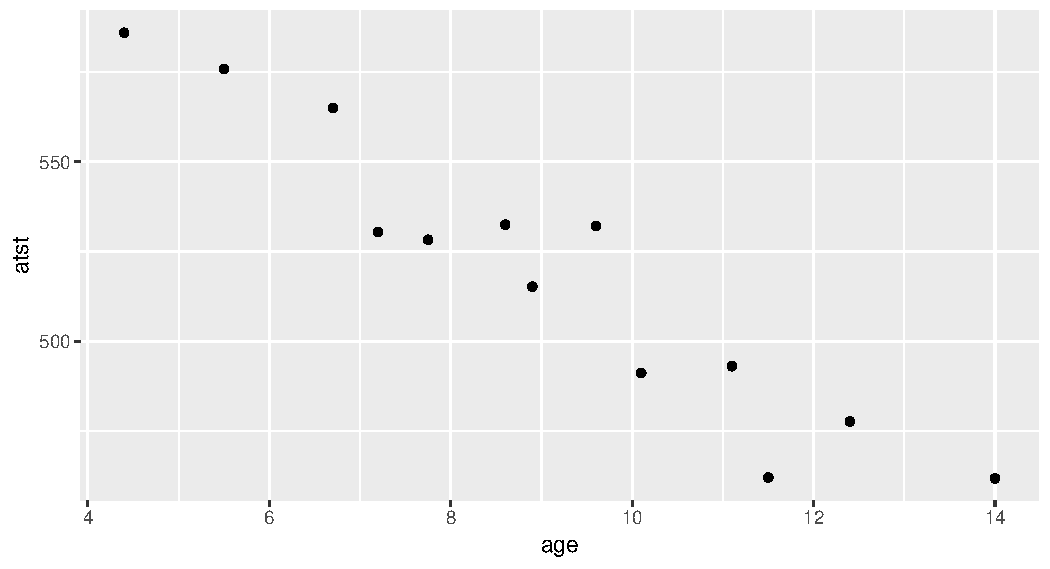
\includegraphics{figure/suggo-1.pdf}
\caption{plot of chunk suggo}
\end{figure}

\end{frame}

\begin{frame}[fragile]{Correlation}
\protect\hypertarget{correlation}{}

\begin{itemize}
\tightlist
\item
  Measures how well a straight line fits the data:
\end{itemize}

\begin{Shaded}
\begin{Highlighting}[]
\KeywordTok{with}\NormalTok{(sleep, }\KeywordTok{cor}\NormalTok{(atst, age))}
\end{Highlighting}
\end{Shaded}

\begin{verbatim}
## [1] -0.9515469
\end{verbatim}

\begin{itemize}
\item
  \(1\) is perfect upward trend, \(-1\) is perfect downward trend, 0 is
  no trend.
\item
  This one close to perfect downward trend.
\item
  Can do correlations of all pairs of variables:
\end{itemize}

\begin{Shaded}
\begin{Highlighting}[]
\KeywordTok{cor}\NormalTok{(sleep)}
\end{Highlighting}
\end{Shaded}

\begin{verbatim}
##            atst        age
## atst  1.0000000 -0.9515469
## age  -0.9515469  1.0000000
\end{verbatim}

\end{frame}

\begin{frame}[fragile]{Lowess curve}
\protect\hypertarget{lowess-curve}{}

\begin{itemize}
\item
  Sometimes nice to guide the eye: is the trend straight, or not?
\item
  Idea: \emph{lowess curve}. ``Locally weighted least squares'', not
  affected by outliers, not constrained to be linear.
\item
  Lowess is a \emph{guide}: even if straight line appropriate, may
  wiggle/bend a little. Looking for \emph{serious} problems with
  linearity.
\item
  Add lowess curve to plot using \texttt{geom\_smooth}:
\end{itemize}

\end{frame}

\begin{frame}[fragile]{Plot with lowess curve}
\protect\hypertarget{plot-with-lowess-curve}{}

\begin{Shaded}
\begin{Highlighting}[]
\KeywordTok{ggplot}\NormalTok{(sleep, }\KeywordTok{aes}\NormalTok{(}\DataTypeTok{x =}\NormalTok{ age, }\DataTypeTok{y =}\NormalTok{ atst)) }\OperatorTok{+}\StringTok{ }\KeywordTok{geom_point}\NormalTok{() }\OperatorTok{+}
\StringTok{  }\KeywordTok{geom_smooth}\NormalTok{()}
\end{Highlighting}
\end{Shaded}

\begin{verbatim}
## `geom_smooth()` using method = 'loess' and formula 'y ~ x'
\end{verbatim}

\begin{figure}
\centering
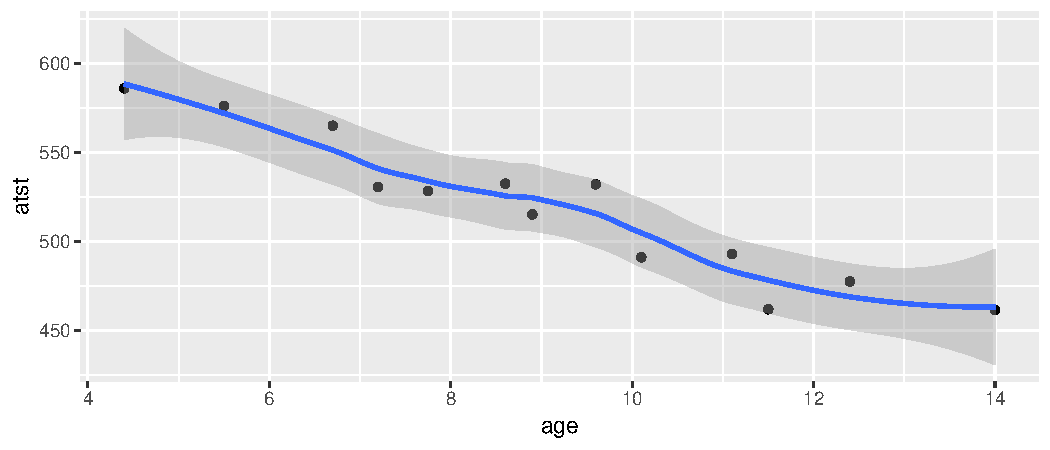
\includegraphics{figure/icko-1.pdf}
\caption{plot of chunk icko}
\end{figure}

\end{frame}

\begin{frame}[fragile]{The regression}
\protect\hypertarget{the-regression}{}

Scatterplot shows no obvious curve, and a pretty clear downward trend.
So we can run the regression:

\begin{Shaded}
\begin{Highlighting}[]
\NormalTok{sleep}\FloatTok{.1}\NormalTok{ <-}\StringTok{ }\KeywordTok{lm}\NormalTok{(atst }\OperatorTok{~}\StringTok{ }\NormalTok{age, }\DataTypeTok{data =}\NormalTok{ sleep)}
\end{Highlighting}
\end{Shaded}

\end{frame}

\begin{frame}[fragile]{The output}
\protect\hypertarget{the-output}{}

\scriptsize

\begin{Shaded}
\begin{Highlighting}[]
\KeywordTok{summary}\NormalTok{(sleep}\FloatTok{.1}\NormalTok{)}
\end{Highlighting}
\end{Shaded}

\begin{verbatim}
## 
## Call:
## lm(formula = atst ~ age, data = sleep)
## 
## Residuals:
##     Min      1Q  Median      3Q     Max 
## -23.011  -9.365   2.372   6.770  20.411 
## 
## Coefficients:
##             Estimate Std. Error t value Pr(>|t|)    
## (Intercept)  646.483     12.918   50.05 2.49e-14 ***
## age          -14.041      1.368  -10.26 5.70e-07 ***
## ---
## Signif. codes:  
## 0 '***' 0.001 '**' 0.01 '*' 0.05 '.' 0.1 ' ' 1
## 
## Residual standard error: 13.15 on 11 degrees of freedom
## Multiple R-squared:  0.9054, Adjusted R-squared:  0.8968 
## F-statistic: 105.3 on 1 and 11 DF,  p-value: 5.7e-07
\end{verbatim}

\normalsize

\end{frame}

\begin{frame}{Conclusions}
\protect\hypertarget{conclusions}{}

\begin{itemize}
\item
  The relationship appears to be a straight line, with a downward trend.
\item
  \(F\)-tests for model as a whole and \(t\)-test for slope (same) both
  confirm this (P-value \(5.7\times 10^{-7}=0.00000057\)).
\item
  Slope is \(-14\), so a 1-year increase in age goes with a 14-minute
  decrease in ATST on average.
\item
  R-squared is correlation squared (when one \(x\) anyway), between 0
  and 1 (1 good, 0 bad).
\item
  Here R-squared is 0.9054, pleasantly high.
\end{itemize}

\end{frame}

\begin{frame}[fragile]{Doing things with the regression output}
\protect\hypertarget{doing-things-with-the-regression-output}{}

\begin{itemize}
\item
  Output from regression (and eg. \(t\)-test) is all right to look at,
  but hard to extract and re-use information from.
\item
  Package \texttt{broom} extracts info from model output in way that can
  be used in pipe (later):
\end{itemize}

\begin{Shaded}
\begin{Highlighting}[]
\KeywordTok{tidy}\NormalTok{(sleep}\FloatTok{.1}\NormalTok{)}
\end{Highlighting}
\end{Shaded}

\begin{verbatim}
## # A tibble: 2 x 5
##   term        estimate std.error statistic  p.value
##   <chr>          <dbl>     <dbl>     <dbl>    <dbl>
## 1 (Intercept)    646.      12.9       50.0 2.49e-14
## 2 age            -14.0      1.37     -10.3 5.70e- 7
\end{verbatim}

\end{frame}

\begin{frame}[fragile]{also one-line summary of model:}
\protect\hypertarget{also-one-line-summary-of-model}{}

\begin{Shaded}
\begin{Highlighting}[]
\KeywordTok{glance}\NormalTok{(sleep}\FloatTok{.1}\NormalTok{)}
\end{Highlighting}
\end{Shaded}

\begin{verbatim}
## # A tibble: 1 x 11
##   r.squared adj.r.squared sigma statistic p.value    df
##       <dbl>         <dbl> <dbl>     <dbl>   <dbl> <int>
## 1     0.905         0.897  13.2      105. 5.70e-7     2
## # … with 5 more variables: logLik <dbl>, AIC <dbl>,
## #   BIC <dbl>, deviance <dbl>, df.residual <int>
\end{verbatim}

\end{frame}

\begin{frame}[fragile]{Broom part 2}
\protect\hypertarget{broom-part-2}{}

\begin{Shaded}
\begin{Highlighting}[]
\NormalTok{sleep}\FloatTok{.1} \OperatorTok\StringTok{ }\KeywordTok{augment}\NormalTok{(sleep) }\OperatorTok\StringTok{ }\KeywordTok{slice}\NormalTok{(}\DecValTok{1}\OperatorTok{:}\DecValTok{8}\NormalTok{)}
\end{Highlighting}
\end{Shaded}

\begin{verbatim}
## # A tibble: 8 x 9
##    atst   age .fitted .se.fit .resid   .hat .sigma .cooksd
##   <dbl> <dbl>   <dbl>   <dbl>  <dbl>  <dbl>  <dbl>   <dbl>
## 1  586    4.4    585.    7.34   1.30 0.312    13.8 0.00320
## 2  462.  14      450.    7.68  11.8  0.341    13.0 0.319  
## 3  491.  10.1    505.    3.92 -13.6  0.0887   13.0 0.0568 
## 4  565    6.7    552.    4.87  12.6  0.137    13.1 0.0844 
## 5  462   11.5    485.    4.95 -23.0  0.141    11.3 0.294  
## 6  532.   9.6    512.    3.72  20.4  0.0801   12.0 0.114  
## 7  478.  12.4    472.    5.85   5.23 0.198    13.7 0.0243 
## 8  515.   8.9    522.    3.65  -6.32 0.0772   13.6 0.0105 
## # … with 1 more variable: .std.resid <dbl>
\end{verbatim}

Useful for plotting residuals against an \(x\)-variable.

\end{frame}

\begin{frame}{CI for mean response and prediction intervals}
\protect\hypertarget{ci-for-mean-response-and-prediction-intervals}{}

Once useful regression exists, use it for prediction:

\begin{itemize}
\item
  To get a single number for prediction at a given \(x\), substitute
  into regression equation, eg. age 10: predicted ATST is
  \(646.48-14.04(10)=506\) minutes.
\item
  To express uncertainty of this prediction:
\item
  \emph{CI for mean response} expresses uncertainty about mean ATST for
  all children aged 10, based on data.
\item
  \emph{Prediction interval} expresses uncertainty about predicted ATST
  for a new child aged 10 whose ATST not known. More uncertain.
\item
  Also do above for a child aged 5.
\end{itemize}

\end{frame}

\begin{frame}[fragile]{Intervals}
\protect\hypertarget{intervals}{}

\begin{itemize}
\tightlist
\item
  Make new data frame with these values for \texttt{age}
\end{itemize}

\begin{Shaded}
\begin{Highlighting}[]
\NormalTok{my.age <-}\StringTok{ }\KeywordTok{c}\NormalTok{(}\DecValTok{10}\NormalTok{, }\DecValTok{5}\NormalTok{)}
\NormalTok{ages.new <-}\StringTok{ }\KeywordTok{tibble}\NormalTok{(}\DataTypeTok{age =}\NormalTok{ my.age)}
\NormalTok{ages.new}
\end{Highlighting}
\end{Shaded}

\begin{verbatim}
## # A tibble: 2 x 1
##     age
##   <dbl>
## 1    10
## 2     5
\end{verbatim}

\begin{itemize}
\tightlist
\item
  Feed into \texttt{predict}:
\end{itemize}

\begin{Shaded}
\begin{Highlighting}[]
\NormalTok{pc <-}\StringTok{ }\KeywordTok{predict}\NormalTok{(sleep}\FloatTok{.1}\NormalTok{, ages.new, }\DataTypeTok{interval =} \StringTok{"c"}\NormalTok{)}
\NormalTok{pp <-}\StringTok{ }\KeywordTok{predict}\NormalTok{(sleep}\FloatTok{.1}\NormalTok{, ages.new, }\DataTypeTok{interval =} \StringTok{"p"}\NormalTok{)}
\end{Highlighting}
\end{Shaded}

\end{frame}

\begin{frame}[fragile]{The intervals}
\protect\hypertarget{the-intervals}{}

Confidence intervals for mean response:

\begin{Shaded}
\begin{Highlighting}[]
\KeywordTok{cbind}\NormalTok{(ages.new, pc)}
\end{Highlighting}
\end{Shaded}

\begin{verbatim}
##   age      fit      lwr      upr
## 1  10 506.0729 497.5574 514.5883
## 2   5 576.2781 561.6578 590.8984
\end{verbatim}

Prediction intervals for new response:

\begin{Shaded}
\begin{Highlighting}[]
\KeywordTok{cbind}\NormalTok{(ages.new, pp)}
\end{Highlighting}
\end{Shaded}

\begin{verbatim}
##   age      fit      lwr      upr
## 1  10 506.0729 475.8982 536.2475
## 2   5 576.2781 543.8474 608.7088
\end{verbatim}

\end{frame}

\begin{frame}[fragile]{Comments}
\protect\hypertarget{comments}{}

\begin{itemize}
\item
  Age 10 closer to centre of data, so intervals are both narrower than
  those for age 5.
\item
  Prediction intervals bigger than CI for mean (additional uncertainty).
\item
  Technical note: output from \texttt{predict} is R \texttt{matrix}, not
  data frame, so Tidyverse \texttt{bind\_cols} does not work. Use base R
  \texttt{cbind}.
\end{itemize}

\end{frame}

\begin{frame}[fragile]{That grey envelope}
\protect\hypertarget{that-grey-envelope}{}

Marks confidence interval for mean for all \(x\):

\begin{Shaded}
\begin{Highlighting}[]
\KeywordTok{ggplot}\NormalTok{(sleep, }\KeywordTok{aes}\NormalTok{(}\DataTypeTok{x =}\NormalTok{ age, }\DataTypeTok{y =}\NormalTok{ atst)) }\OperatorTok{+}\StringTok{ }\KeywordTok{geom_point}\NormalTok{() }\OperatorTok{+}
\StringTok{  }\KeywordTok{geom_smooth}\NormalTok{(}\DataTypeTok{method =} \StringTok{"lm"}\NormalTok{) }\OperatorTok{+}
\StringTok{  }\KeywordTok{scale_y_continuous}\NormalTok{(}\DataTypeTok{breaks =} \KeywordTok{seq}\NormalTok{(}\DecValTok{420}\NormalTok{, }\DecValTok{600}\NormalTok{, }\DecValTok{20}\NormalTok{))}
\end{Highlighting}
\end{Shaded}

\begin{figure}
\centering
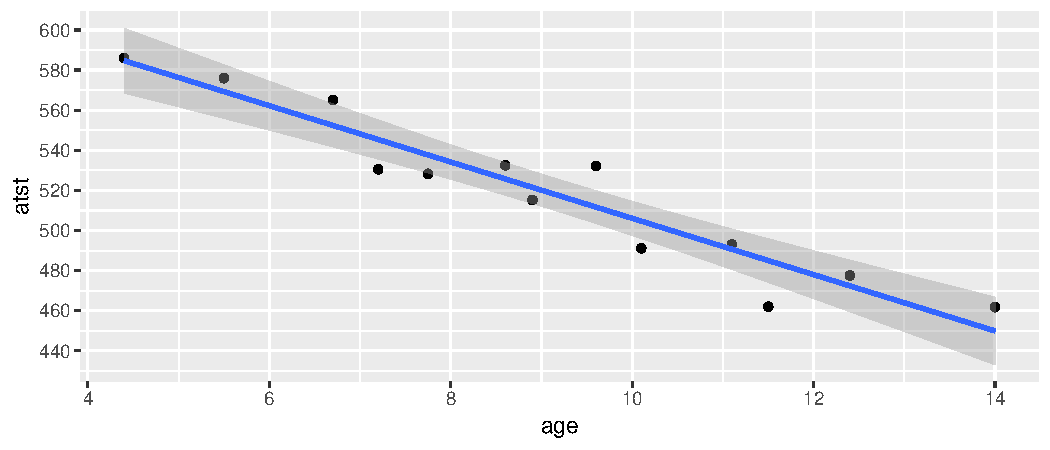
\includegraphics{figure/unnamed-chunk-17-1.pdf}
\caption{plot of chunk unnamed-chunk-17}
\end{figure}

\end{frame}

\begin{frame}{Diagnostics}
\protect\hypertarget{diagnostics}{}

How to tell whether a straight-line regression is appropriate?

\vspace{3ex}

\begin{itemize}
\item
  Before: check scatterplot for straight trend.
\item
  After: plot \emph{residuals} (observed minus predicted response)
  against predicted values. Aim: a plot with no pattern.
\end{itemize}

\end{frame}

\begin{frame}[fragile]{Residual plot}
\protect\hypertarget{residual-plot}{}

Not much pattern here --- regression appropriate.

\begin{Shaded}
\begin{Highlighting}[]
\KeywordTok{ggplot}\NormalTok{(sleep}\FloatTok{.1}\NormalTok{, }\KeywordTok{aes}\NormalTok{(}\DataTypeTok{x =}\NormalTok{ .fitted, }\DataTypeTok{y =}\NormalTok{ .resid)) }\OperatorTok{+}\StringTok{ }\KeywordTok{geom_point}\NormalTok{()}
\end{Highlighting}
\end{Shaded}

\begin{figure}
\centering
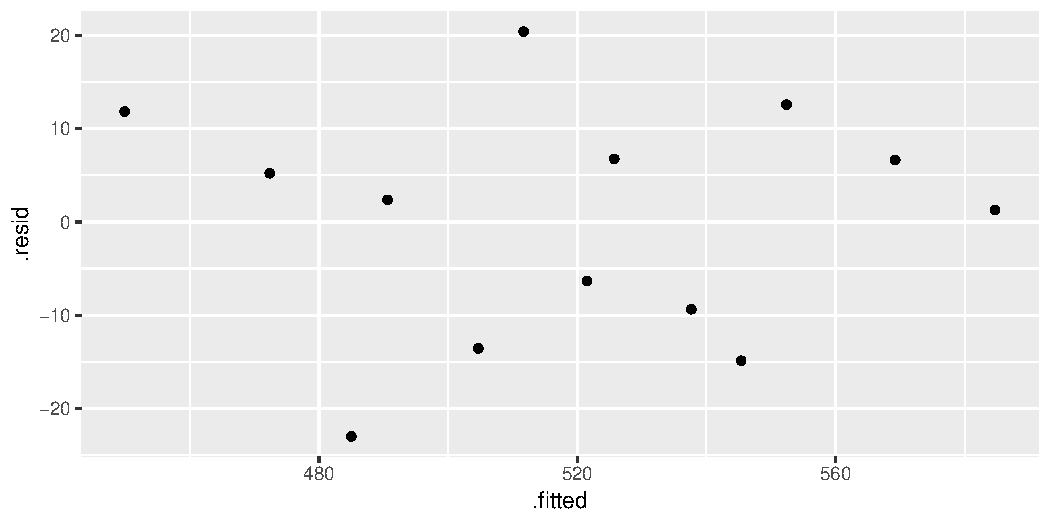
\includegraphics{figure/akjhkadjfhjahnkkk-1.pdf}
\caption{plot of chunk akjhkadjfhjahnkkk}
\end{figure}

\end{frame}

\begin{frame}[fragile]{An inappropriate regression}
\protect\hypertarget{an-inappropriate-regression}{}

Different data:

\begin{Shaded}
\begin{Highlighting}[]
\NormalTok{my_url <-}\StringTok{ "http://www.utsc.utoronto.ca/~butler/d29/curvy.txt"}
\NormalTok{curvy <-}\StringTok{ }\KeywordTok{read_delim}\NormalTok{(my_url, }\StringTok{" "}\NormalTok{)}
\end{Highlighting}
\end{Shaded}

\begin{verbatim}
## Parsed with column specification:
## cols(
##   xx = col_double(),
##   yy = col_double()
## )
\end{verbatim}

\end{frame}

\begin{frame}[fragile]{Scatterplot}
\protect\hypertarget{scatterplot}{}

\begin{Shaded}
\begin{Highlighting}[]
\KeywordTok{ggplot}\NormalTok{(curvy, }\KeywordTok{aes}\NormalTok{(}\DataTypeTok{x =}\NormalTok{ xx, }\DataTypeTok{y =}\NormalTok{ yy)) }\OperatorTok{+}\StringTok{ }\KeywordTok{geom_point}\NormalTok{()}
\end{Highlighting}
\end{Shaded}

\begin{figure}
\centering
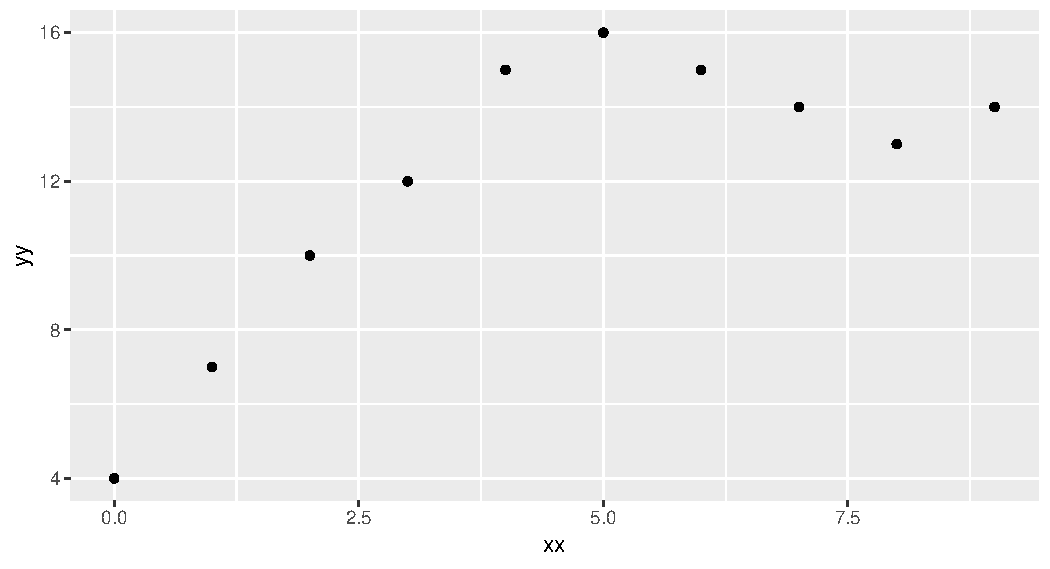
\includegraphics{figure/unnamed-chunk-18-1.pdf}
\caption{plot of chunk unnamed-chunk-18}
\end{figure}

\end{frame}

\begin{frame}[fragile]{Regression line, anyway}
\protect\hypertarget{regression-line-anyway}{}

\scriptsize

\begin{Shaded}
\begin{Highlighting}[]
\NormalTok{curvy}\FloatTok{.1}\NormalTok{ <-}\StringTok{ }\KeywordTok{lm}\NormalTok{(yy }\OperatorTok{~}\StringTok{ }\NormalTok{xx, }\DataTypeTok{data =}\NormalTok{ curvy)}
\KeywordTok{summary}\NormalTok{(curvy}\FloatTok{.1}\NormalTok{)}
\end{Highlighting}
\end{Shaded}

\begin{verbatim}
## 
## Call:
## lm(formula = yy ~ xx, data = curvy)
## 
## Residuals:
##    Min     1Q Median     3Q    Max 
## -3.582 -2.204  0.000  1.514  3.509 
## 
## Coefficients:
##             Estimate Std. Error t value Pr(>|t|)   
## (Intercept)   7.5818     1.5616   4.855  0.00126 **
## xx            0.9818     0.2925   3.356  0.00998 **
## ---
## Signif. codes:  
## 0 '***' 0.001 '**' 0.01 '*' 0.05 '.' 0.1 ' ' 1
## 
## Residual standard error: 2.657 on 8 degrees of freedom
## Multiple R-squared:  0.5848, Adjusted R-squared:  0.5329 
## F-statistic: 11.27 on 1 and 8 DF,  p-value: 0.009984
\end{verbatim}

\normalsize

\end{frame}

\begin{frame}[fragile]{Residual plot}
\protect\hypertarget{residual-plot-1}{}

\begin{Shaded}
\begin{Highlighting}[]
\KeywordTok{ggplot}\NormalTok{(curvy}\FloatTok{.1}\NormalTok{, }\KeywordTok{aes}\NormalTok{(}\DataTypeTok{x =}\NormalTok{ .fitted, }\DataTypeTok{y =}\NormalTok{ .resid)) }\OperatorTok{+}\StringTok{ }\KeywordTok{geom_point}\NormalTok{()}
\end{Highlighting}
\end{Shaded}

\begin{figure}
\centering
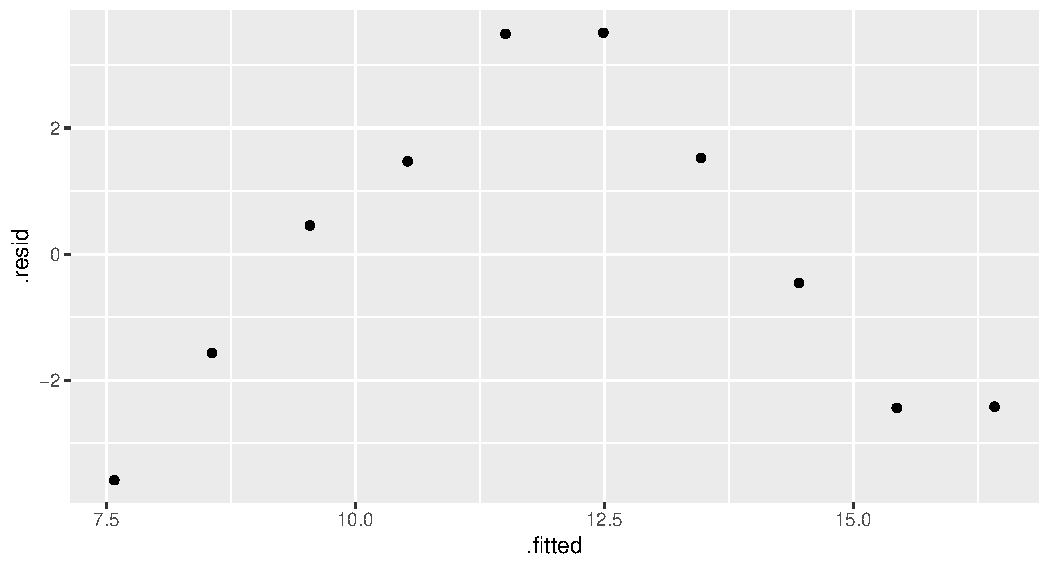
\includegraphics{figure/altoadige-1.pdf}
\caption{plot of chunk altoadige}
\end{figure}

\end{frame}

\begin{frame}[fragile]{No good: fixing it up}
\protect\hypertarget{no-good-fixing-it-up}{}

\begin{itemize}
\item
  Residual plot has \emph{curve}: middle residuals positive, high and
  low ones negative. Bad.
\item
  Fitting a curve would be better. Try this:
\end{itemize}

\begin{Shaded}
\begin{Highlighting}[]
\NormalTok{curvy}\FloatTok{.2}\NormalTok{ <-}\StringTok{ }\KeywordTok{lm}\NormalTok{(yy }\OperatorTok{~}\StringTok{ }\NormalTok{xx }\OperatorTok{+}\StringTok{ }\KeywordTok{I}\NormalTok{(xx}\OperatorTok{^}\DecValTok{2}\NormalTok{), }\DataTypeTok{data =}\NormalTok{ curvy)}
\end{Highlighting}
\end{Shaded}

\begin{itemize}
\item
  Adding \texttt{xx}-squared term, to allow for curve.
\item
  Another way to do same thing: specify how model \emph{changes}:
\end{itemize}

\begin{Shaded}
\begin{Highlighting}[]
\NormalTok{curvy}\FloatTok{.2}\NormalTok{a <-}\StringTok{ }\KeywordTok{update}\NormalTok{(curvy}\FloatTok{.1}\NormalTok{, . }\OperatorTok{~}\StringTok{ }\NormalTok{. }\OperatorTok{+}\StringTok{ }\KeywordTok{I}\NormalTok{(xx}\OperatorTok{^}\DecValTok{2}\NormalTok{))}
\end{Highlighting}
\end{Shaded}

\end{frame}

\begin{frame}[fragile]{Regression 2}
\protect\hypertarget{regression-2}{}

\begin{Shaded}
\begin{Highlighting}[]
\KeywordTok{tidy}\NormalTok{(curvy}\FloatTok{.2}\NormalTok{)}
\end{Highlighting}
\end{Shaded}

\begin{verbatim}
## # A tibble: 3 x 5
##   term        estimate std.error statistic   p.value
##   <chr>          <dbl>     <dbl>     <dbl>     <dbl>
## 1 (Intercept)    3.9      0.773       5.04 0.00149  
## 2 xx             3.74     0.400       9.36 0.0000331
## 3 I(xx^2)       -0.307    0.0428     -7.17 0.000182
\end{verbatim}

\begin{Shaded}
\begin{Highlighting}[]
\KeywordTok{glance}\NormalTok{(curvy}\FloatTok{.2}\NormalTok{) }\CommentTok{#}
\end{Highlighting}
\end{Shaded}

\begin{verbatim}
## # A tibble: 1 x 11
##   r.squared adj.r.squared sigma statistic p.value    df
##       <dbl>         <dbl> <dbl>     <dbl>   <dbl> <int>
## 1     0.950         0.936 0.983      66.8 2.75e-5     3
## # … with 5 more variables: logLik <dbl>, AIC <dbl>,
## #   BIC <dbl>, deviance <dbl>, df.residual <int>
\end{verbatim}

\end{frame}

\begin{frame}[fragile]{Comments}
\protect\hypertarget{comments-1}{}

\begin{itemize}
\item
  \texttt{xx}-squared term definitely significant (P-value 0.000182), so
  need this curve to describe relationship.
\item
  Adding squared term has made R-squared go up from 0.5848 to 0.9502:
  great improvement.
\item
  This is a definite curve!
\end{itemize}

\end{frame}

\begin{frame}[fragile]{The residual plot now}
\protect\hypertarget{the-residual-plot-now}{}

No problems any more:

\begin{Shaded}
\begin{Highlighting}[]
\KeywordTok{ggplot}\NormalTok{(curvy}\FloatTok{.2}\NormalTok{, }\KeywordTok{aes}\NormalTok{(}\DataTypeTok{x =}\NormalTok{ .fitted, }\DataTypeTok{y =}\NormalTok{ .resid)) }\OperatorTok{+}\StringTok{ }\KeywordTok{geom_point}\NormalTok{()}
\end{Highlighting}
\end{Shaded}

\begin{figure}
\centering
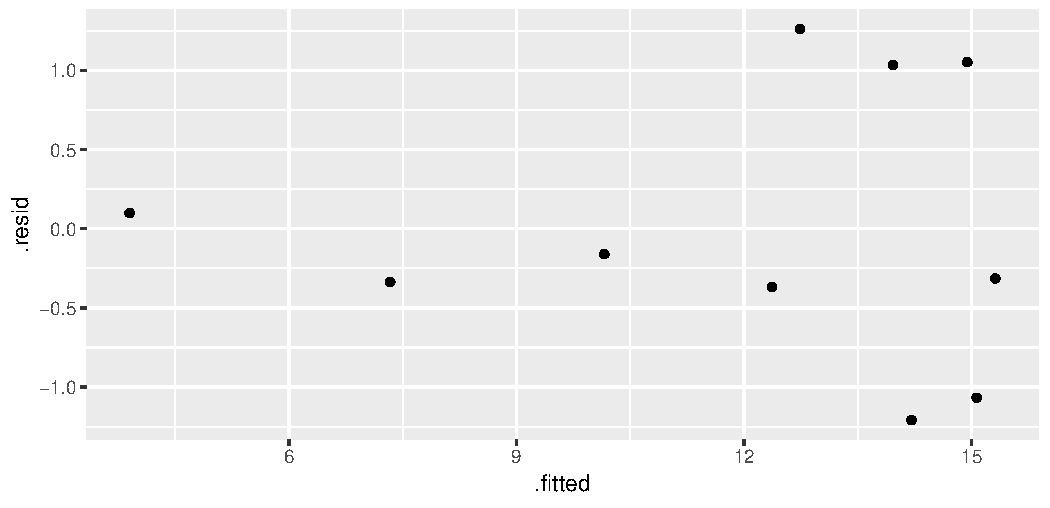
\includegraphics{figure/unnamed-chunk-23-1.pdf}
\caption{plot of chunk unnamed-chunk-23}
\end{figure}

\end{frame}

\begin{frame}{Another way to handle curves}
\protect\hypertarget{another-way-to-handle-curves}{}

\begin{itemize}
\item
  Above, saw that changing \(x\) (adding \(x^2\)) was a way of handling
  curved relationships.
\item
  Another way: change \(y\) (transformation).
\item
  Can guess how to change \(y\), or might be theory:
\item
  example: relationship \(y=ae^{bx}\) (exponential growth):
\item
  take logs to get \(\ln y=\ln a + bx\).
\item
  Taking logs has made relationship linear (\(\ln y\) as response).
\item
  Or, \emph{estimate} transformation, using Box-Cox method.
\end{itemize}

\end{frame}

\begin{frame}[fragile]{Box-Cox}
\protect\hypertarget{box-cox}{}

\begin{itemize}
\item
  Install package \texttt{MASS} via \texttt{install.packages("MASS")}
  (only need to do \emph{once})
\item
  Every R session you want to use something in \texttt{MASS}, type
  \texttt{library(MASS)}
\end{itemize}

\end{frame}

\begin{frame}[fragile]{Some made-up data}
\protect\hypertarget{some-made-up-data}{}

\begin{Shaded}
\begin{Highlighting}[]
\NormalTok{my_url <-}\StringTok{ "http://www.utsc.utoronto.ca/~butler/d29/madeup.csv"}
\NormalTok{madeup <-}\StringTok{ }\KeywordTok{read_csv}\NormalTok{(my_url)}
\NormalTok{madeup}
\end{Highlighting}
\end{Shaded}

\begin{verbatim}
## # A tibble: 8 x 3
##     row     x     y
##   <dbl> <dbl> <dbl>
## 1     1     0  17.9
## 2     2     1  33.6
## 3     3     2  82.7
## 4     4     3  31.2
## 5     5     4 177. 
## 6     6     5 359. 
## 7     7     6 469. 
## 8     8     7 583.
\end{verbatim}

Seems to be faster-than-linear growth, maybe exponential growth.

\end{frame}

\begin{frame}[fragile]{Scatterplot: faster than linear growth}
\protect\hypertarget{scatterplot-faster-than-linear-growth}{}

\begin{Shaded}
\begin{Highlighting}[]
\KeywordTok{ggplot}\NormalTok{(madeup, }\KeywordTok{aes}\NormalTok{(}\DataTypeTok{x =}\NormalTok{ x, }\DataTypeTok{y =}\NormalTok{ y)) }\OperatorTok{+}\StringTok{ }\KeywordTok{geom_point}\NormalTok{() }\OperatorTok{+}
\StringTok{  }\KeywordTok{geom_smooth}\NormalTok{()}
\end{Highlighting}
\end{Shaded}

\begin{verbatim}
## `geom_smooth()` using method = 'loess' and formula 'y ~ x'
\end{verbatim}

\begin{figure}
\centering
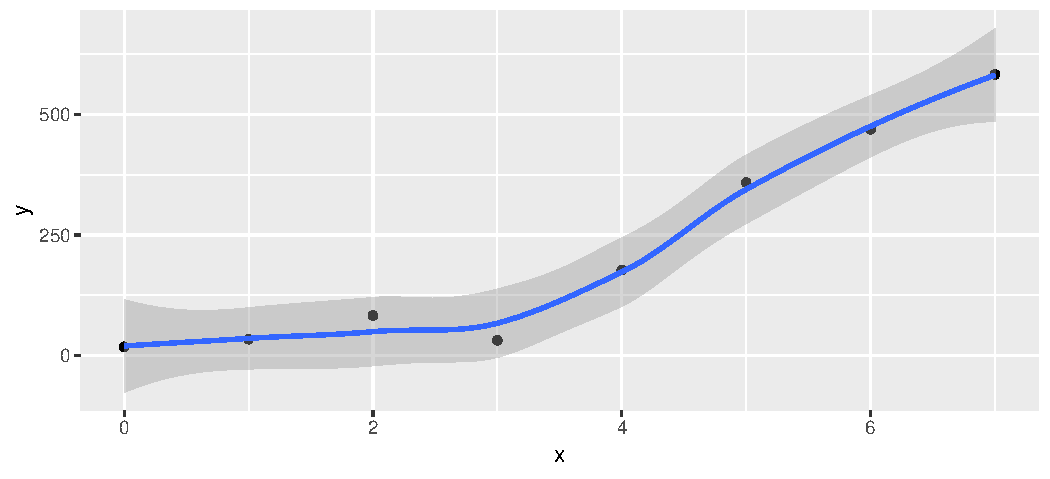
\includegraphics{figure/dsljhsdjlhf-1.pdf}
\caption{plot of chunk dsljhsdjlhf}
\end{figure}

\end{frame}

\begin{frame}[fragile]{Running Box-Cox}
\protect\hypertarget{running-box-cox}{}

\begin{itemize}
\item
  \texttt{library(MASS)} first.
\item
  Feed \texttt{boxcox} a model formula with a squiggle in it, such as
  you would use for \texttt{lm}.
\item
  Output: a graph (next page):
\end{itemize}

\begin{Shaded}
\begin{Highlighting}[]
\KeywordTok{boxcox}\NormalTok{(y }\OperatorTok{~}\StringTok{ }\NormalTok{x, }\DataTypeTok{data =}\NormalTok{ madeup)}
\end{Highlighting}
\end{Shaded}

\end{frame}

\begin{frame}{The Box-Cox output}
\protect\hypertarget{the-box-cox-output}{}

\begin{figure}
\centering
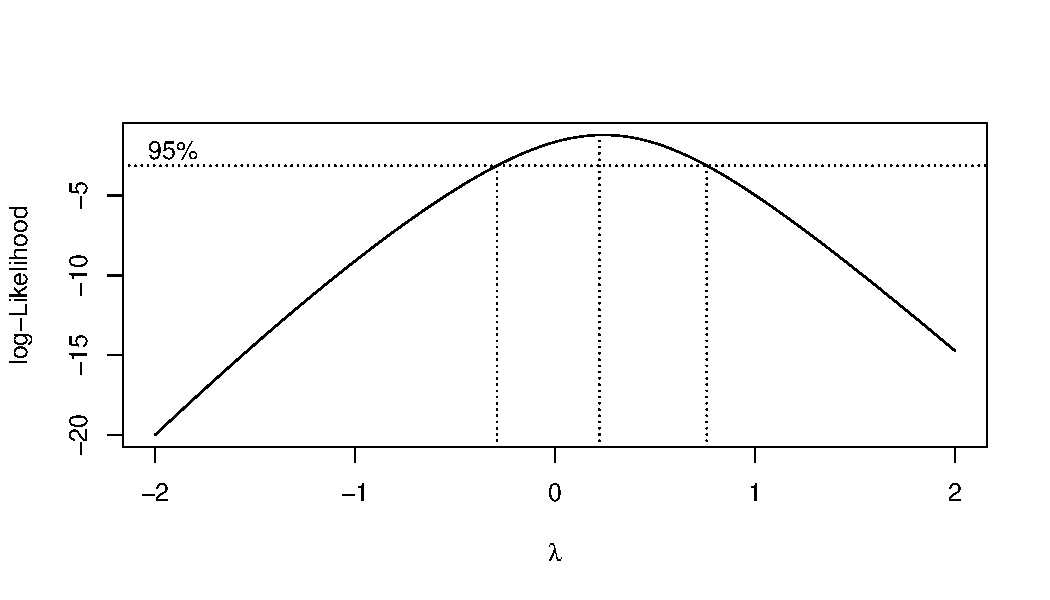
\includegraphics{figure/trento-1.pdf}
\caption{plot of chunk trento}
\end{figure}

\end{frame}

\begin{frame}{Comments}
\protect\hypertarget{comments-2}{}

\begin{itemize}
\item
  \(\lambda\) (lambda) is the power by which you should transform \(y\)
  to get the relationship straight (straighter). Power 0 is ``take
  logs''
\item
  Middle dotted line marks best single value of \(\lambda\) (here about
  0.1).
\item
  Outer dotted lines mark 95\% CI for \(\lambda\), here \(-0.3\) to 0.7,
  approx. (Rather uncertain about best transformation.)
\item
  Any power transformation within the CI supported by data. In this
  case, log (\(\lambda=0\)) and square root (\(\lambda=0.5\)) good, but
  no transformation (\(\lambda=1\)) not.
\item
  Pick a ``round-number'' value of \(\lambda\) like
  \(2,1,0.5,0,-0.5,-1\). Here 0 and 0.5 good values to pick.
\end{itemize}

\end{frame}

\begin{frame}[fragile]{Did transformation straighten things?}
\protect\hypertarget{did-transformation-straighten-things}{}

\begin{itemize}
\tightlist
\item
  Plot transformed \(y\) against \(x\). Here, log:
\end{itemize}

\begin{Shaded}
\begin{Highlighting}[]
\KeywordTok{ggplot}\NormalTok{(madeup, }\KeywordTok{aes}\NormalTok{(}\DataTypeTok{x =}\NormalTok{ x, }\DataTypeTok{y =} \KeywordTok{log}\NormalTok{(y))) }\OperatorTok{+}\StringTok{ }\KeywordTok{geom_point}\NormalTok{() }\OperatorTok{+}
\StringTok{  }\KeywordTok{geom_smooth}\NormalTok{()}
\end{Highlighting}
\end{Shaded}

\begin{figure}
\centering
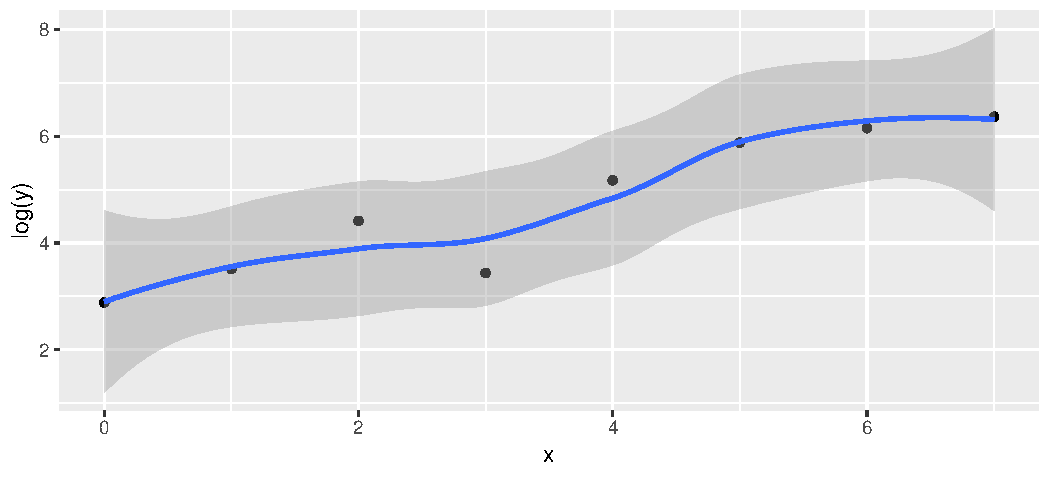
\includegraphics{figure/unnamed-chunk-26-1.pdf}
\caption{plot of chunk unnamed-chunk-26}
\end{figure}

Looks much straighter.

\end{frame}

\begin{frame}[fragile]{Regression with transformed \(y\)}
\protect\hypertarget{regression-with-transformed-y}{}

\footnotesize

\begin{Shaded}
\begin{Highlighting}[]
\NormalTok{madeup}\FloatTok{.1}\NormalTok{ <-}\StringTok{ }\KeywordTok{lm}\NormalTok{(}\KeywordTok{log}\NormalTok{(y) }\OperatorTok{~}\StringTok{ }\NormalTok{x, }\DataTypeTok{data =}\NormalTok{ madeup)}
\KeywordTok{glance}\NormalTok{(madeup}\FloatTok{.1}\NormalTok{)}
\end{Highlighting}
\end{Shaded}

\begin{verbatim}
## # A tibble: 1 x 11
##   r.squared adj.r.squared sigma statistic p.value    df
##       <dbl>         <dbl> <dbl>     <dbl>   <dbl> <int>
## 1     0.883         0.864 0.501      45.3 5.24e-4     2
## # … with 5 more variables: logLik <dbl>, AIC <dbl>,
## #   BIC <dbl>, deviance <dbl>, df.residual <int>
\end{verbatim}

\begin{Shaded}
\begin{Highlighting}[]
\KeywordTok{tidy}\NormalTok{(madeup}\FloatTok{.1}\NormalTok{)}
\end{Highlighting}
\end{Shaded}

\begin{verbatim}
## # A tibble: 2 x 5
##   term        estimate std.error statistic  p.value
##   <chr>          <dbl>     <dbl>     <dbl>    <dbl>
## 1 (Intercept)    2.91     0.323       8.99 0.000106
## 2 x              0.520    0.0773      6.73 0.000524
\end{verbatim}

\normalsize

R-squared now decently high.

\end{frame}

\begin{frame}[fragile]{Multiple regression}
\protect\hypertarget{multiple-regression}{}

\begin{itemize}
\item
  What if more than one \(x\)? Extra issues:

  \begin{itemize}
  \item
    Now one intercept and a slope for each \(x\): how to interpret?
  \item
    Which \(x\)-variables actually help to predict \(y\)?
  \item
    Different interpretations of ``global'' \(F\)-test and individual
    \(t\)-tests.
  \item
    R-squared no longer correlation squared, but still interpreted as
    ``higher better''.
  \item
    In \texttt{lm} line, add extra \(x\)s after
    \texttt{\textasciitilde{}}.
  \item
    Interpretation not so easy (and other problems that can occur).
  \end{itemize}
\end{itemize}

\end{frame}

\begin{frame}[fragile]{Multiple regression example}
\protect\hypertarget{multiple-regression-example}{}

Study of women and visits to health professionals, and how the number of
visits might be related to other variables:

\begin{description}
\item[timedrs:] number of visits to health professionals (over course of study)
\item[phyheal:] number of physical health problems
\item[menheal:] number of mental health problems
\item[stress:] result of questionnaire about number and type of life changes
\end{description}

\texttt{timedrs} response, others explanatory.

\end{frame}

\begin{frame}[fragile]{The data}
\protect\hypertarget{the-data}{}

\begin{Shaded}
\begin{Highlighting}[]
\NormalTok{my_url <-}\StringTok{ }
\StringTok{  "http://www.utsc.utoronto.ca/~butler/d29/regressx.txt"}
\NormalTok{visits <-}\StringTok{ }\KeywordTok{read_delim}\NormalTok{(my_url, }\StringTok{" "}\NormalTok{)}
\end{Highlighting}
\end{Shaded}

\begin{verbatim}
## Parsed with column specification:
## cols(
##   subjno = col_double(),
##   timedrs = col_double(),
##   phyheal = col_double(),
##   menheal = col_double(),
##   stress = col_double()
## )
\end{verbatim}

\end{frame}

\begin{frame}[fragile]{Check data}
\protect\hypertarget{check-data-1}{}

\small

\begin{Shaded}
\begin{Highlighting}[]
\NormalTok{visits}
\end{Highlighting}
\end{Shaded}

\begin{verbatim}
## # A tibble: 465 x 5
##    subjno timedrs phyheal menheal stress
##     <dbl>   <dbl>   <dbl>   <dbl>  <dbl>
##  1      1       1       5       8    265
##  2      2       3       4       6    415
##  3      3       0       3       4     92
##  4      4      13       2       2    241
##  5      5      15       3       6     86
##  6      6       3       5       5    247
##  7      7       2       5       6     13
##  8      8       0       4       5     12
##  9      9       7       5       4    269
## 10     10       4       3       9    391
## # … with 455 more rows
\end{verbatim}

\normalsize

\end{frame}

\begin{frame}[fragile]{Fit multiple regression}
\protect\hypertarget{fit-multiple-regression}{}

\begin{Shaded}
\begin{Highlighting}[]
\NormalTok{visits}\FloatTok{.1}\NormalTok{ <-}\StringTok{ }\KeywordTok{lm}\NormalTok{(timedrs }\OperatorTok{~}\StringTok{ }\NormalTok{phyheal }\OperatorTok{+}\StringTok{ }\NormalTok{menheal }\OperatorTok{+}\StringTok{ }\NormalTok{stress,}
  \DataTypeTok{data =}\NormalTok{ visits)}
\KeywordTok{glance}\NormalTok{(visits}\FloatTok{.1}\NormalTok{)}
\end{Highlighting}
\end{Shaded}

\begin{verbatim}
## # A tibble: 1 x 11
##   r.squared adj.r.squared sigma statistic  p.value    df
##       <dbl>         <dbl> <dbl>     <dbl>    <dbl> <int>
## 1     0.219         0.214  9.71      43.0 1.56e-24     4
## # … with 5 more variables: logLik <dbl>, AIC <dbl>,
## #   BIC <dbl>, deviance <dbl>, df.residual <int>
\end{verbatim}

\end{frame}

\begin{frame}[fragile]{The slopes}
\protect\hypertarget{the-slopes}{}

Model as a whole strongly significant even though R-sq not very big
(lots of data). At least one of the \(x\)'s predicts \texttt{timedrs}.

\begin{Shaded}
\begin{Highlighting}[]
\KeywordTok{tidy}\NormalTok{(visits}\FloatTok{.1}\NormalTok{)}
\end{Highlighting}
\end{Shaded}

\begin{verbatim}
## # A tibble: 4 x 5
##   term        estimate std.error statistic  p.value
##   <chr>          <dbl>     <dbl>     <dbl>    <dbl>
## 1 (Intercept) -3.70      1.12      -3.30   1.06e- 3
## 2 phyheal      1.79      0.221      8.08   5.60e-15
## 3 menheal     -0.00967   0.129     -0.0749 9.40e- 1
## 4 stress       0.0136    0.00361    3.77   1.85e- 4
\end{verbatim}

The physical health and stress variables initely help to predict the
number of visits, but \emph{with those in the model} we don't need
\texttt{menheal}. However, look at prediction of \texttt{timedrs} from
\texttt{menheal} by itself:

\end{frame}

\begin{frame}[fragile]{Just \texttt{menheal}}
\protect\hypertarget{just-menheal}{}

\footnotesize

\begin{Shaded}
\begin{Highlighting}[]
\NormalTok{visits}\FloatTok{.2}\NormalTok{ <-}\StringTok{ }\KeywordTok{lm}\NormalTok{(timedrs }\OperatorTok{~}\StringTok{ }\NormalTok{menheal, }\DataTypeTok{data =}\NormalTok{ visits)}
\KeywordTok{glance}\NormalTok{(visits}\FloatTok{.2}\NormalTok{)}
\end{Highlighting}
\end{Shaded}

\begin{verbatim}
## # A tibble: 1 x 11
##   r.squared adj.r.squared sigma statistic p.value    df
##       <dbl>         <dbl> <dbl>     <dbl>   <dbl> <int>
## 1    0.0653        0.0633  10.6      32.4 2.28e-8     2
## # … with 5 more variables: logLik <dbl>, AIC <dbl>,
## #   BIC <dbl>, deviance <dbl>, df.residual <int>
\end{verbatim}

\begin{Shaded}
\begin{Highlighting}[]
\KeywordTok{tidy}\NormalTok{(visits}\FloatTok{.2}\NormalTok{)}
\end{Highlighting}
\end{Shaded}

\begin{verbatim}
## # A tibble: 2 x 5
##   term        estimate std.error statistic      p.value
##   <chr>          <dbl>     <dbl>     <dbl>        <dbl>
## 1 (Intercept)    3.82      0.870      4.38 0.0000144   
## 2 menheal        0.667     0.117      5.69 0.0000000228
\end{verbatim}

\normalsize

\end{frame}

\begin{frame}[fragile]{\texttt{menheal} by itself}
\protect\hypertarget{menheal-by-itself}{}

\begin{itemize}
\item
  \texttt{menheal} by itself \emph{does} significantly help to predict
  \texttt{timedrs}.
\item
  But the R-sq is much less (6.5\% vs.~22\%).
\item
  So other two variables do a better job of prediction.
\item
  With those variables in the regression (\texttt{phyheal} and
  \texttt{stress}), don't need \texttt{menheal} \emph{as well}.
\end{itemize}

\end{frame}

\begin{frame}[fragile]{Investigating via correlation}
\protect\hypertarget{investigating-via-correlation}{}

Leave out first column (\texttt{subjno}):

\begin{Shaded}
\begin{Highlighting}[]
\NormalTok{visits }\OperatorTok\StringTok{ }\KeywordTok{select}\NormalTok{(}\OperatorTok{-}\NormalTok{subjno) }\OperatorTok\StringTok{ }\KeywordTok{cor}\NormalTok{()}
\end{Highlighting}
\end{Shaded}

\begin{verbatim}
##           timedrs   phyheal   menheal    stress
## timedrs 1.0000000 0.4395293 0.2555703 0.2865951
## phyheal 0.4395293 1.0000000 0.5049464 0.3055517
## menheal 0.2555703 0.5049464 1.0000000 0.3697911
## stress  0.2865951 0.3055517 0.3697911 1.0000000
\end{verbatim}

\begin{itemize}
\item
  \texttt{phyheal} most strongly correlated with \texttt{timedrs}.
\item
  Not much to choose between other two.
\item
  But \texttt{menheal} has higher correlation with \texttt{phyheal}, so
  not as much to \emph{add} to prediction as \texttt{stress}.
\item
  Goes to show things more complicated in multiple regression.
\end{itemize}

\end{frame}

\begin{frame}[fragile]{Residual plot (from \texttt{timedrs} on all)}
\protect\hypertarget{residual-plot-from-timedrs-on-all}{}

\begin{Shaded}
\begin{Highlighting}[]
\KeywordTok{ggplot}\NormalTok{(visits}\FloatTok{.1}\NormalTok{, }\KeywordTok{aes}\NormalTok{(}\DataTypeTok{x =}\NormalTok{ .fitted, }\DataTypeTok{y =}\NormalTok{ .resid)) }\OperatorTok{+}\StringTok{ }\KeywordTok{geom_point}\NormalTok{()}
\end{Highlighting}
\end{Shaded}

\begin{figure}
\centering
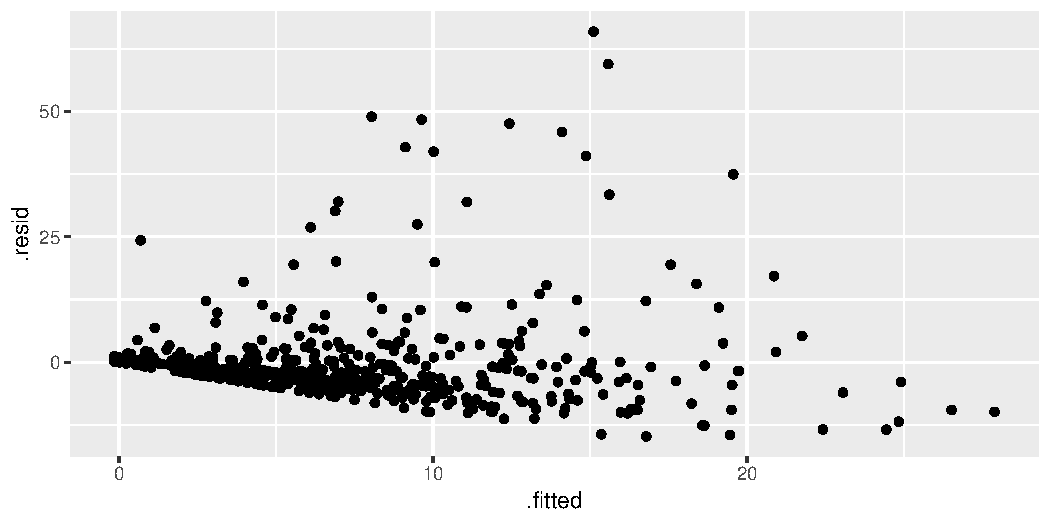
\includegraphics{figure/iffy8-1.pdf}
\caption{plot of chunk iffy8}
\end{figure}

\end{frame}

\begin{frame}{Comment}
\protect\hypertarget{comment}{}

Apparently random. But\ldots

\end{frame}

\begin{frame}[fragile]{Normal quantile plot of residuals}
\protect\hypertarget{normal-quantile-plot-of-residuals}{}

\begin{Shaded}
\begin{Highlighting}[]
\KeywordTok{ggplot}\NormalTok{(visits}\FloatTok{.1}\NormalTok{, }\KeywordTok{aes}\NormalTok{(}\DataTypeTok{sample =}\NormalTok{ .resid)) }\OperatorTok{+}\StringTok{ }\KeywordTok{stat_qq}\NormalTok{() }\OperatorTok{+}\StringTok{ }\KeywordTok{stat_qq_line}\NormalTok{()}
\end{Highlighting}
\end{Shaded}

\begin{figure}
\centering
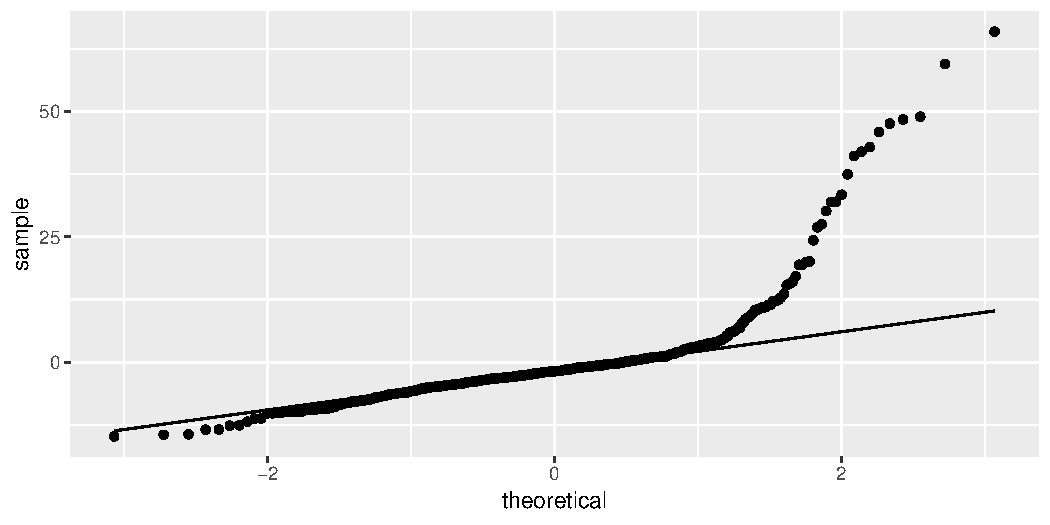
\includegraphics{figure/unnamed-chunk-34-1.pdf}
\caption{plot of chunk unnamed-chunk-34}
\end{figure}

\end{frame}

\begin{frame}[fragile]{Absolute residuals}
\protect\hypertarget{absolute-residuals}{}

Is there trend in \emph{size} of residuals (fan-out)? Plot
\emph{absolute value} of residual against fitted value (graph next
page):

\begin{Shaded}
\begin{Highlighting}[]
\NormalTok{g <-}\StringTok{ }\KeywordTok{ggplot}\NormalTok{(visits}\FloatTok{.1}\NormalTok{, }\KeywordTok{aes}\NormalTok{(}\DataTypeTok{x =}\NormalTok{ .fitted, }\DataTypeTok{y =} \KeywordTok{abs}\NormalTok{(.resid))) }\OperatorTok{+}
\StringTok{  }\KeywordTok{geom_point}\NormalTok{() }\OperatorTok{+}\StringTok{ }\KeywordTok{geom_smooth}\NormalTok{()}
\end{Highlighting}
\end{Shaded}

\end{frame}

\begin{frame}{The plot}
\protect\hypertarget{the-plot}{}

\begin{figure}
\centering
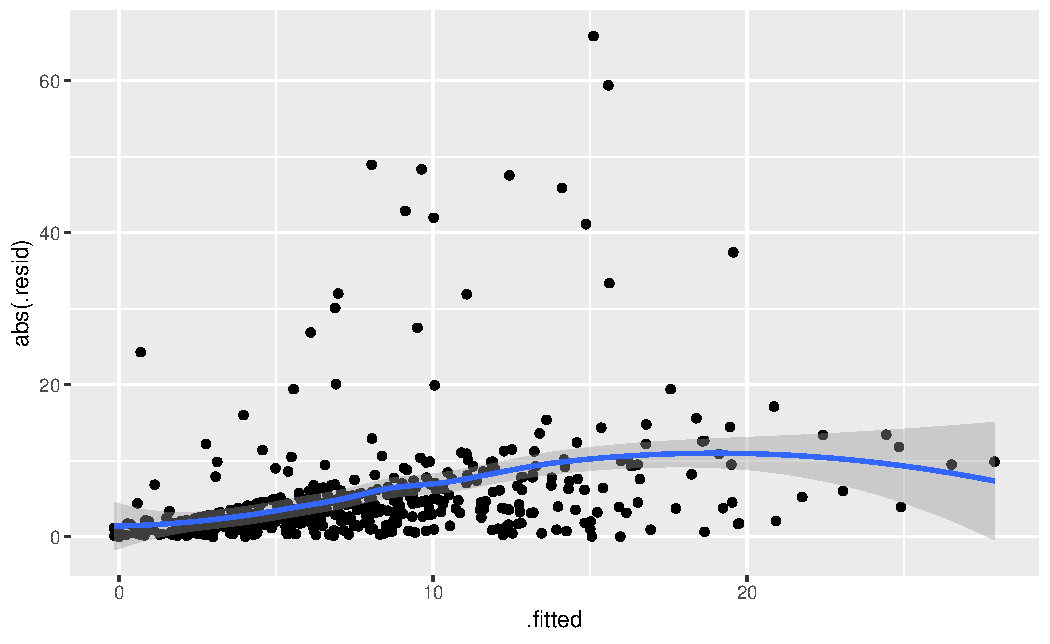
\includegraphics{figure/unnamed-chunk-36-1.pdf}
\caption{plot of chunk unnamed-chunk-36}
\end{figure}

\end{frame}

\begin{frame}[fragile]{Comments}
\protect\hypertarget{comments-3}{}

\begin{itemize}
\item
  On the normal quantile plot:

  \begin{itemize}
  \item
    highest (most positive) residuals are \emph{way} too high
  \item
    distribution of residuals skewed to right (not normal at all)
  \end{itemize}
\item
  On plot of absolute residuals:

  \begin{itemize}
  \item
    size of residuals getting bigger as fitted values increase
  \item
    predictions getting more variable as fitted values increase
  \item
    that is, predictions getting \emph{less accurate} as fitted values
    increase, but predictions should be equally accurate all way along.
  \end{itemize}
\item
  Both indicate problems with regression, of kind that transformation of
  response often fixes: that is, predict \emph{function} of response
  \texttt{timedrs} instead of \texttt{timedrs} itself.
\end{itemize}

\end{frame}

\begin{frame}[fragile]{Box-Cox transformations}
\protect\hypertarget{box-cox-transformations}{}

\begin{itemize}
\item
  Taking log of \texttt{timedrs} and having it work: lucky guess. How to
  find good transformation?
\item
  Box-Cox again.
\item
  Extra problem: some of \texttt{timedrs} values are 0, but Box-Cox
  expects all +. Note response for \texttt{boxcox}:
\end{itemize}

\begin{Shaded}
\begin{Highlighting}[]
\KeywordTok{boxcox}\NormalTok{(timedrs }\OperatorTok{+}\StringTok{ }\DecValTok{1} \OperatorTok{~}\StringTok{ }\NormalTok{phyheal }\OperatorTok{+}\StringTok{ }\NormalTok{menheal }\OperatorTok{+}\StringTok{ }\NormalTok{stress, }\DataTypeTok{data =}\NormalTok{ visits)}
\end{Highlighting}
\end{Shaded}

\end{frame}

\begin{frame}{Try 1}
\protect\hypertarget{try-1}{}

\begin{figure}
\centering
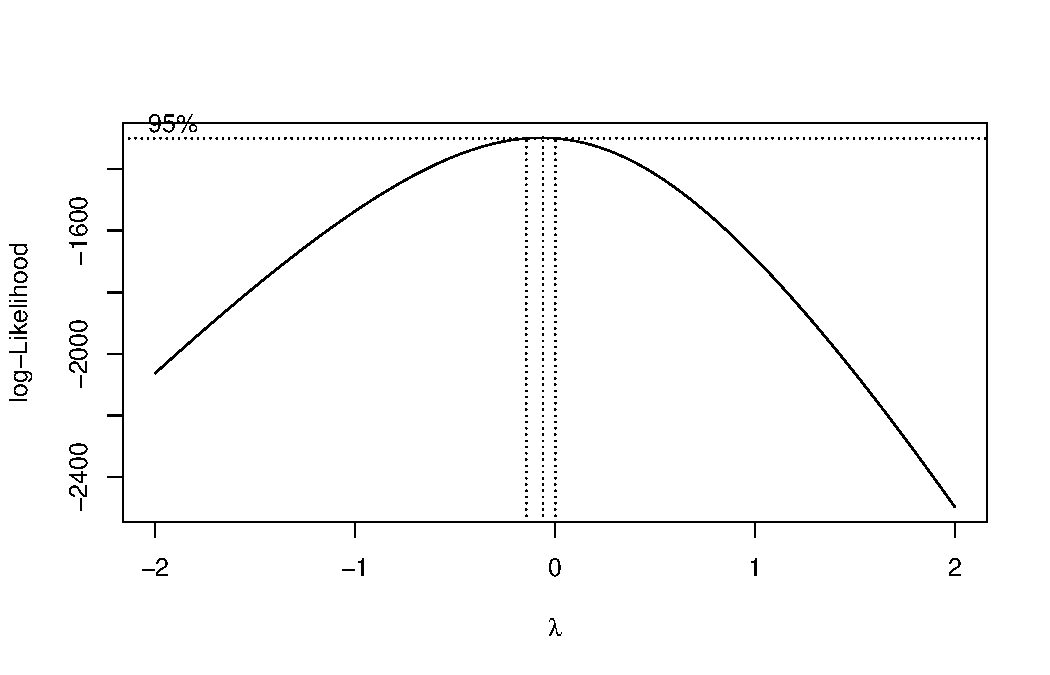
\includegraphics{figure/unnamed-chunk-38-1.pdf}
\caption{plot of chunk unnamed-chunk-38}
\end{figure}

\end{frame}

\begin{frame}[fragile]{Comments on try 1}
\protect\hypertarget{comments-on-try-1}{}

\begin{itemize}
\item
  Best: \(\lambda\) just less than zero.
\item
  Hard to see scale.
\item
  Focus on \(\lambda\) in \((-0.3,0.1)\):
\end{itemize}

\footnotesize

\begin{Shaded}
\begin{Highlighting}[]
\NormalTok{my.lambda <-}\StringTok{ }\KeywordTok{seq}\NormalTok{(}\OperatorTok{-}\FloatTok{0.3}\NormalTok{, }\FloatTok{0.1}\NormalTok{, }\FloatTok{0.01}\NormalTok{)}
\NormalTok{my.lambda}
\end{Highlighting}
\end{Shaded}

\begin{verbatim}
##  [1] -0.30 -0.29 -0.28 -0.27 -0.26 -0.25 -0.24 -0.23 -0.22
## [10] -0.21 -0.20 -0.19 -0.18 -0.17 -0.16 -0.15 -0.14 -0.13
## [19] -0.12 -0.11 -0.10 -0.09 -0.08 -0.07 -0.06 -0.05 -0.04
## [28] -0.03 -0.02 -0.01  0.00  0.01  0.02  0.03  0.04  0.05
## [37]  0.06  0.07  0.08  0.09  0.10
\end{verbatim}

\normalsize

\end{frame}

\begin{frame}[fragile]{Try 2}
\protect\hypertarget{try-2}{}

\begin{Shaded}
\begin{Highlighting}[]
\KeywordTok{boxcox}\NormalTok{(timedrs }\OperatorTok{+}\StringTok{ }\DecValTok{1} \OperatorTok{~}\StringTok{ }\NormalTok{phyheal }\OperatorTok{+}\StringTok{ }\NormalTok{menheal }\OperatorTok{+}\StringTok{ }\NormalTok{stress,}
  \DataTypeTok{lambda =}\NormalTok{ my.lambda,}
  \DataTypeTok{data =}\NormalTok{ visits}
\NormalTok{)}
\end{Highlighting}
\end{Shaded}

\begin{figure}
\centering
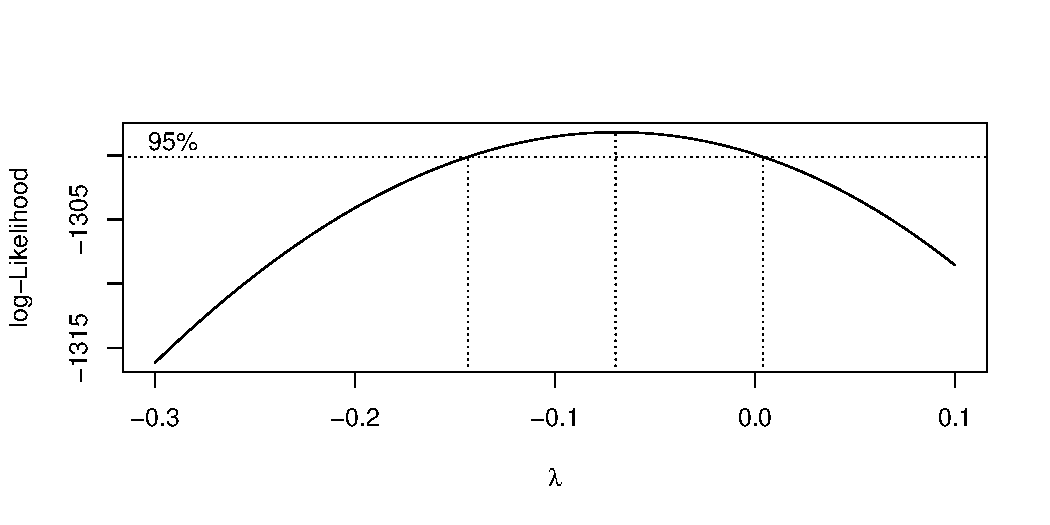
\includegraphics{figure/unnamed-chunk-40-1.pdf}
\caption{plot of chunk unnamed-chunk-40}
\end{figure}

\end{frame}

\begin{frame}{Comments}
\protect\hypertarget{comments-4}{}

\begin{itemize}
\item
  Best: \(\lambda\) just about \(-0.07\).
\item
  CI for \(\lambda\) about \((-0.14,0.01)\).
\item
  Only nearby round number: \(\lambda=0\), log transformation.
\end{itemize}

\end{frame}

\begin{frame}[fragile]{Fixing the problems}
\protect\hypertarget{fixing-the-problems}{}

\begin{itemize}
\item
  Try regression again, with transformed response instead of original
  one.
\item
  Then check residual plot to see that it is OK now.
\end{itemize}

\begin{Shaded}
\begin{Highlighting}[]
\NormalTok{visits}\FloatTok{.3}\NormalTok{ <-}\StringTok{ }\KeywordTok{lm}\NormalTok{(}\KeywordTok{log}\NormalTok{(timedrs }\OperatorTok{+}\StringTok{ }\DecValTok{1}\NormalTok{) }\OperatorTok{~}\StringTok{ }\NormalTok{phyheal }\OperatorTok{+}\StringTok{ }\NormalTok{menheal }\OperatorTok{+}\StringTok{ }\NormalTok{stress,}
  \DataTypeTok{data =}\NormalTok{ visits}
\NormalTok{)}
\end{Highlighting}
\end{Shaded}

\begin{itemize}
\item
  \texttt{timedrs+1} because some \texttt{timedrs} values 0, can't take
  log of 0.
\item
  Won't usually need to worry about this, but when response could be
  zero/negative, fix that before transformation.
\end{itemize}

\end{frame}

\begin{frame}[fragile]{Output}
\protect\hypertarget{output}{}

\scriptsize

\begin{Shaded}
\begin{Highlighting}[]
\KeywordTok{summary}\NormalTok{(visits}\FloatTok{.3}\NormalTok{)}
\end{Highlighting}
\end{Shaded}

\begin{verbatim}
## 
## Call:
## lm(formula = log(timedrs + 1) ~ phyheal + menheal + stress, data = visits)
## 
## Residuals:
##      Min       1Q   Median       3Q      Max 
## -1.95865 -0.44076 -0.02331  0.42304  2.36797 
## 
## Coefficients:
##              Estimate Std. Error t value Pr(>|t|)    
## (Intercept) 0.3903862  0.0882908   4.422 1.22e-05 ***
## phyheal     0.2019361  0.0173624  11.631  < 2e-16 ***
## menheal     0.0071442  0.0101335   0.705    0.481    
## stress      0.0013158  0.0002837   4.638 4.58e-06 ***
## ---
## Signif. codes:  
## 0 '***' 0.001 '**' 0.01 '*' 0.05 '.' 0.1 ' ' 1
## 
## Residual standard error: 0.7625 on 461 degrees of freedom
## Multiple R-squared:  0.3682, Adjusted R-squared:  0.3641 
## F-statistic: 89.56 on 3 and 461 DF,  p-value: < 2.2e-16
\end{verbatim}

\normalsize

\end{frame}

\begin{frame}[fragile]{Comments}
\protect\hypertarget{comments-5}{}

\begin{itemize}
\item
  Model as a whole strongly significant again
\item
  R-sq higher than before (37\% vs.~22\%) suggesting things more linear
  now
\item
  Same conclusion re \texttt{menheal}: can take out of regression.
\item
  Should look at residual plots (next pages). Have we fixed problems?
\end{itemize}

\end{frame}

\begin{frame}[fragile]{Residuals against fitted values}
\protect\hypertarget{residuals-against-fitted-values}{}

\begin{Shaded}
\begin{Highlighting}[]
\KeywordTok{ggplot}\NormalTok{(visits}\FloatTok{.3}\NormalTok{, }\KeywordTok{aes}\NormalTok{(}\DataTypeTok{x =}\NormalTok{ .fitted, }\DataTypeTok{y =}\NormalTok{ .resid)) }\OperatorTok{+}
\StringTok{  }\KeywordTok{geom_point}\NormalTok{()}
\end{Highlighting}
\end{Shaded}

\begin{figure}
\centering
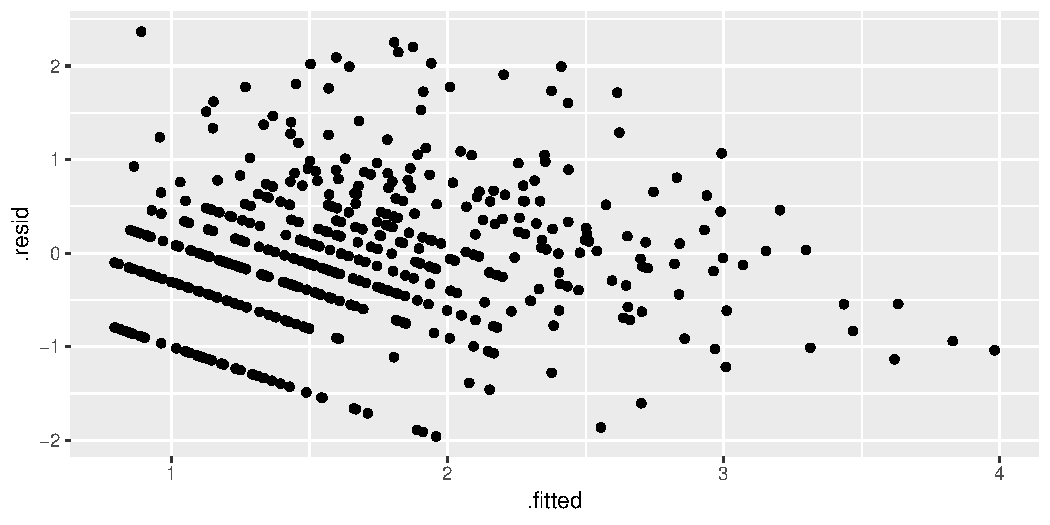
\includegraphics{figure/unnamed-chunk-43-1.pdf}
\caption{plot of chunk unnamed-chunk-43}
\end{figure}

\end{frame}

\begin{frame}[fragile]{Normal quantile plot of residuals}
\protect\hypertarget{normal-quantile-plot-of-residuals-1}{}

\begin{Shaded}
\begin{Highlighting}[]
\KeywordTok{ggplot}\NormalTok{(visits}\FloatTok{.3}\NormalTok{, }\KeywordTok{aes}\NormalTok{(}\DataTypeTok{sample =}\NormalTok{ .resid)) }\OperatorTok{+}\StringTok{ }\KeywordTok{stat_qq}\NormalTok{() }\OperatorTok{+}\StringTok{ }\KeywordTok{stat_qq_line}\NormalTok{()}
\end{Highlighting}
\end{Shaded}

\begin{figure}
\centering
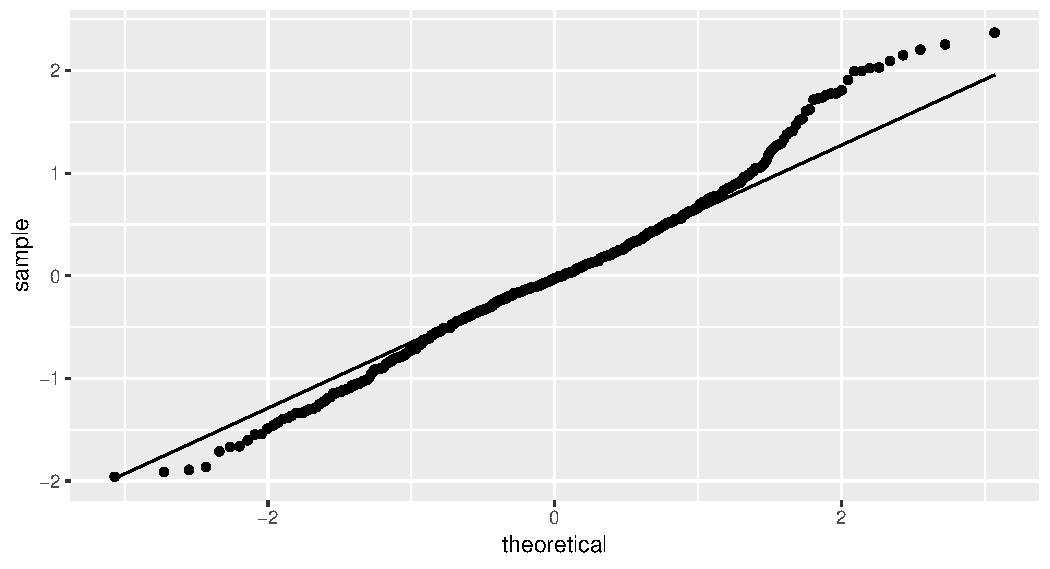
\includegraphics{figure/unnamed-chunk-44-1.pdf}
\caption{plot of chunk unnamed-chunk-44}
\end{figure}

\end{frame}

\begin{frame}[fragile]{Absolute residuals against fitted}
\protect\hypertarget{absolute-residuals-against-fitted}{}

\begin{Shaded}
\begin{Highlighting}[]
\KeywordTok{ggplot}\NormalTok{(visits}\FloatTok{.3}\NormalTok{, }\KeywordTok{aes}\NormalTok{(}\DataTypeTok{x =}\NormalTok{ .fitted, }\DataTypeTok{y =} \KeywordTok{abs}\NormalTok{(.resid))) }\OperatorTok{+}
\StringTok{  }\KeywordTok{geom_point}\NormalTok{() }\OperatorTok{+}\StringTok{ }\KeywordTok{geom_smooth}\NormalTok{()}
\end{Highlighting}
\end{Shaded}

\begin{figure}
\centering
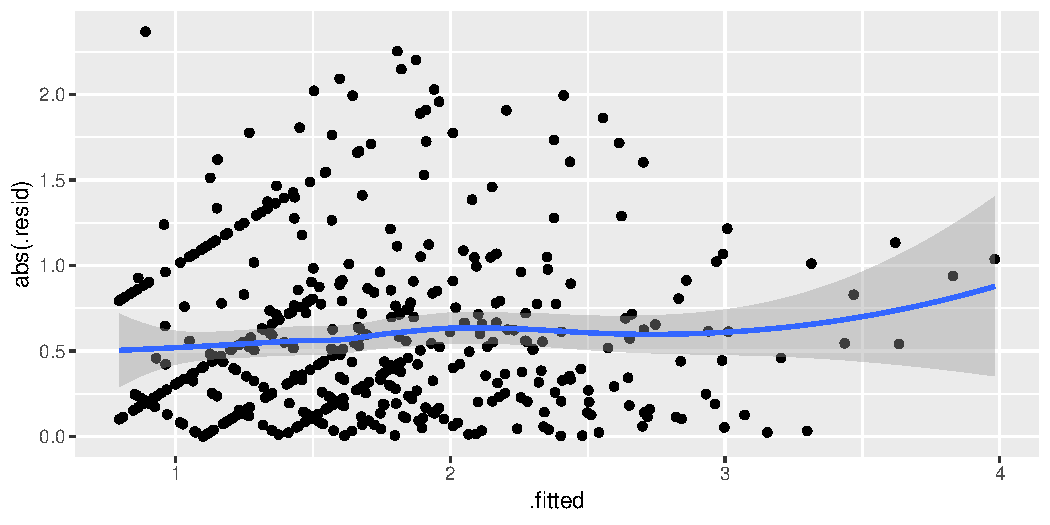
\includegraphics{figure/unnamed-chunk-45-1.pdf}
\caption{plot of chunk unnamed-chunk-45}
\end{figure}

\end{frame}

\begin{frame}{Comments}
\protect\hypertarget{comments-6}{}

\begin{itemize}
\item
  Residuals vs.~fitted looks a lot more random.
\item
  Normal quantile plot looks a lot more normal (though still a little
  right-skewness)
\item
  Absolute residuals: not so much trend (though still some).
\item
  Not perfect, but much improved.
\end{itemize}

\end{frame}

\begin{frame}[fragile]{Testing more than one \(x\) at once}
\protect\hypertarget{testing-more-than-one-x-at-once}{}

\begin{itemize}
\tightlist
\item
  The \(t\)-tests test only whether one variable could be taken out of
  the regression you're looking at.
\item
  To test significance of more than one variable at once, fit model with
  and without variables

  \begin{itemize}
  \tightlist
  \item
    then use \texttt{anova} to compare fit of models:
  \end{itemize}
\end{itemize}

\begin{Shaded}
\begin{Highlighting}[]
\NormalTok{visits}\FloatTok{.5}\NormalTok{ <-}\StringTok{ }\KeywordTok{lm}\NormalTok{(}\KeywordTok{log}\NormalTok{(timedrs }\OperatorTok{+}\StringTok{ }\DecValTok{1}\NormalTok{) }\OperatorTok{~}\StringTok{ }\NormalTok{phyheal }\OperatorTok{+}\StringTok{ }\NormalTok{menheal }\OperatorTok{+}\StringTok{ }\NormalTok{stress, }
               \DataTypeTok{data =}\NormalTok{ visits)}
\NormalTok{visits}\FloatTok{.6}\NormalTok{ <-}\StringTok{ }\KeywordTok{lm}\NormalTok{(}\KeywordTok{log}\NormalTok{(timedrs }\OperatorTok{+}\StringTok{ }\DecValTok{1}\NormalTok{) }\OperatorTok{~}\StringTok{ }\NormalTok{stress, }\DataTypeTok{data =}\NormalTok{ visits)}
\end{Highlighting}
\end{Shaded}

\end{frame}

\begin{frame}[fragile]{Results of tests}
\protect\hypertarget{results-of-tests}{}

\begin{Shaded}
\begin{Highlighting}[]
\KeywordTok{anova}\NormalTok{(visits}\FloatTok{.6}\NormalTok{, visits}\FloatTok{.5}\NormalTok{)}
\end{Highlighting}
\end{Shaded}

\begin{verbatim}
## Analysis of Variance Table
## 
## Model 1: log(timedrs + 1) ~ stress
## Model 2: log(timedrs + 1) ~ phyheal + menheal + stress
##   Res.Df    RSS Df Sum of Sq      F    Pr(>F)    
## 1    463 371.47                                  
## 2    461 268.01  2    103.46 88.984 < 2.2e-16 ***
## ---
## Signif. codes:  
## 0 '***' 0.001 '**' 0.01 '*' 0.05 '.' 0.1 ' ' 1
\end{verbatim}

\begin{itemize}
\item
  Models don't fit equally well, so bigger one fits better.
\item
  Or ``taking both variables out makes the fit worse, so don't do it''.
\item
  Taking out those \(x\)'s is a mistake. Or putting them in is a good
  idea.
\end{itemize}

\end{frame}

\begin{frame}[fragile]{The punting data}
\protect\hypertarget{the-punting-data}{}

Data set \texttt{punting.txt} contains 4 variables for 13 right-footed
football kickers (punters): left leg and right leg strength (lbs),
distance punted (ft), another variable called ``fred''. Predict punting
distance from other variables:

\scriptsize

\begin{verbatim}
left            right               punt         fred
170               170                162.50       171 
130               140                144.0        136   
170               180                174.50       174 
160               160                163.50       161 
150               170                192.0        159 
150               150                171.75       151 
180               170                162.0        174 
110               110                104.83       111 
110               120                105.67       114 
120               130                117.58       126 
140               120                140.25       129  
130               140                150.17       136 
150               160                165.17       154 
\end{verbatim}

\normalsize

\end{frame}

\begin{frame}[fragile]{Reading in}
\protect\hypertarget{reading-in}{}

\begin{itemize}
\tightlist
\item
  Separated by \emph{multiple spaces} with \emph{columns lined up}:
\end{itemize}

\begin{Shaded}
\begin{Highlighting}[]
\NormalTok{my_url <-}\StringTok{ "http://www.utsc.utoronto.ca/~butler/d29/punting.txt"}
\NormalTok{punting <-}\StringTok{ }\KeywordTok{read_table}\NormalTok{(my_url)}
\end{Highlighting}
\end{Shaded}

\begin{verbatim}
## Parsed with column specification:
## cols(
##   left = col_double(),
##   right = col_double(),
##   punt = col_double(),
##   fred = col_double()
## )
\end{verbatim}

\end{frame}

\begin{frame}[fragile]{The data}
\protect\hypertarget{the-data-1}{}

\small

\begin{Shaded}
\begin{Highlighting}[]
\NormalTok{punting}
\end{Highlighting}
\end{Shaded}

\begin{verbatim}
## # A tibble: 13 x 4
##     left right  punt  fred
##    <dbl> <dbl> <dbl> <dbl>
##  1   170   170  162.   171
##  2   130   140  144    136
##  3   170   180  174.   174
##  4   160   160  164.   161
##  5   150   170  192    159
##  6   150   150  172.   151
##  7   180   170  162    174
##  8   110   110  105.   111
##  9   110   120  106.   114
## 10   120   130  118.   126
## 11   140   120  140.   129
## 12   130   140  150.   136
## 13   150   160  165.   154
\end{verbatim}

\normalsize

\end{frame}

\begin{frame}[fragile]{Regression and output}
\protect\hypertarget{regression-and-output}{}

\small

\begin{Shaded}
\begin{Highlighting}[]
\NormalTok{punting}\FloatTok{.1}\NormalTok{ <-}\StringTok{ }\KeywordTok{lm}\NormalTok{(punt }\OperatorTok{~}\StringTok{ }\NormalTok{left }\OperatorTok{+}\StringTok{ }\NormalTok{right }\OperatorTok{+}\StringTok{ }\NormalTok{fred, }\DataTypeTok{data =}\NormalTok{ punting)}
\KeywordTok{glance}\NormalTok{(punting}\FloatTok{.1}\NormalTok{)}
\end{Highlighting}
\end{Shaded}

\begin{verbatim}
## # A tibble: 1 x 11
##   r.squared adj.r.squared sigma statistic p.value    df
##       <dbl>         <dbl> <dbl>     <dbl>   <dbl> <int>
## 1     0.778         0.704  14.7      10.5 0.00267     4
## # … with 5 more variables: logLik <dbl>, AIC <dbl>,
## #   BIC <dbl>, deviance <dbl>, df.residual <int>
\end{verbatim}

\begin{Shaded}
\begin{Highlighting}[]
\KeywordTok{tidy}\NormalTok{(punting}\FloatTok{.1}\NormalTok{)}
\end{Highlighting}
\end{Shaded}

\begin{verbatim}
## # A tibble: 4 x 5
##   term        estimate std.error statistic p.value
##   <chr>          <dbl>     <dbl>     <dbl>   <dbl>
## 1 (Intercept)   -4.69      29.1    -0.161    0.876
## 2 left           0.268      2.11    0.127    0.902
## 3 right          1.05       2.15    0.490    0.636
## 4 fred          -0.267      4.23   -0.0632   0.951
\end{verbatim}

\normalsize

\end{frame}

\begin{frame}{Comments}
\protect\hypertarget{comments-7}{}

\begin{itemize}
\item
  Overall regression strongly significant, R-sq high.
\item
  None of the \(x\)'s significant! Why?
\item
  \(t\)-tests only say that you could take any one of the \(x\)'s out
  without damaging the fit; doesn't matter which one.
\item
  Explanation: look at \emph{correlations}.
\end{itemize}

\end{frame}

\begin{frame}[fragile]{The correlations}
\protect\hypertarget{the-correlations}{}

\begin{Shaded}
\begin{Highlighting}[]
\KeywordTok{cor}\NormalTok{(punting)}
\end{Highlighting}
\end{Shaded}

\begin{verbatim}
##            left     right      punt      fred
## left  1.0000000 0.8957224 0.8117368 0.9722632
## right 0.8957224 1.0000000 0.8805469 0.9728784
## punt  0.8117368 0.8805469 1.0000000 0.8679507
## fred  0.9722632 0.9728784 0.8679507 1.0000000
\end{verbatim}

\begin{itemize}
\item
  \emph{All} correlations are high: \(x\)'s with \texttt{punt} (good)
  and with each other (bad, at least confusing).
\item
  What to do? Probably do just as well to pick one variable, say
  \texttt{right} since kickers are right-footed.
\end{itemize}

\end{frame}

\begin{frame}[fragile]{Just \texttt{right}}
\protect\hypertarget{just-right}{}

\small

\begin{Shaded}
\begin{Highlighting}[]
\NormalTok{punting}\FloatTok{.2}\NormalTok{ <-}\StringTok{ }\KeywordTok{lm}\NormalTok{(punt }\OperatorTok{~}\StringTok{ }\NormalTok{right, }\DataTypeTok{data =}\NormalTok{ punting)}
\KeywordTok{anova}\NormalTok{(punting}\FloatTok{.2}\NormalTok{, punting}\FloatTok{.1}\NormalTok{)}
\end{Highlighting}
\end{Shaded}

\begin{verbatim}
## Analysis of Variance Table
## 
## Model 1: punt ~ right
## Model 2: punt ~ left + right + fred
##   Res.Df    RSS Df Sum of Sq      F Pr(>F)
## 1     11 1962.5                           
## 2      9 1938.2  2    24.263 0.0563 0.9456
\end{verbatim}

\normalsize

No significant loss by dropping other two variables.

\end{frame}

\begin{frame}[fragile]{Comparing R-squareds}
\protect\hypertarget{comparing-r-squareds}{}

\begin{Shaded}
\begin{Highlighting}[]
\KeywordTok{summary}\NormalTok{(punting}\FloatTok{.1}\NormalTok{)}\OperatorTok{$}\NormalTok{r.squared}
\end{Highlighting}
\end{Shaded}

\begin{verbatim}
## [1] 0.7781401
\end{verbatim}

\begin{Shaded}
\begin{Highlighting}[]
\KeywordTok{summary}\NormalTok{(punting}\FloatTok{.2}\NormalTok{)}\OperatorTok{$}\NormalTok{r.squared}
\end{Highlighting}
\end{Shaded}

\begin{verbatim}
## [1] 0.7753629
\end{verbatim}

Basically no difference. In regression (over), \texttt{right}
significant:

\end{frame}

\begin{frame}[fragile]{Regression results}
\protect\hypertarget{regression-results}{}

\begin{Shaded}
\begin{Highlighting}[]
\KeywordTok{tidy}\NormalTok{(punting}\FloatTok{.2}\NormalTok{)}
\end{Highlighting}
\end{Shaded}

\begin{verbatim}
## # A tibble: 2 x 5
##   term        estimate std.error statistic   p.value
##   <chr>          <dbl>     <dbl>     <dbl>     <dbl>
## 1 (Intercept)    -3.69    25.3      -0.146 0.886    
## 2 right           1.04     0.169     6.16  0.0000709
\end{verbatim}

\end{frame}

\begin{frame}[fragile]{But\ldots}
\protect\hypertarget{but}{}

\begin{itemize}
\item
  Maybe we got the \emph{form} of the relationship with \texttt{left}
  wrong.
\item
  Check: plot \emph{residuals} from previous regression (without
  \texttt{left}) against \texttt{left}.
\item
  Residuals here are ``punting distance adjusted for right leg
  strength''.
\item
  If there is some kind of relationship with \texttt{left}, we should
  include in model.
\item
  Plot of residuals against original variable: \texttt{augment} from
  \texttt{broom}.
\end{itemize}

\end{frame}

\begin{frame}[fragile]{Augmenting \texttt{punting.2}}
\protect\hypertarget{augmenting-punting.2}{}

\footnotesize

\begin{Shaded}
\begin{Highlighting}[]
\NormalTok{punting}\FloatTok{.2} \OperatorTok\StringTok{ }\KeywordTok{augment}\NormalTok{(punting) ->}\StringTok{ }\NormalTok{punting.}\FloatTok{2.}\NormalTok{aug}
\NormalTok{punting.}\FloatTok{2.}\NormalTok{aug }\OperatorTok\StringTok{ }\KeywordTok{slice}\NormalTok{(}\DecValTok{1}\OperatorTok{:}\DecValTok{8}\NormalTok{)}
\end{Highlighting}
\end{Shaded}

\begin{verbatim}
## # A tibble: 8 x 11
##    left right  punt  fred .fitted .se.fit  .resid   .hat
##   <dbl> <dbl> <dbl> <dbl>   <dbl>   <dbl>   <dbl>  <dbl>
## 1   170   170  162.   171    174.    5.29 -11.1   0.157 
## 2   130   140  144    136    142.    3.93   1.72  0.0864
## 3   170   180  174.   174    184.    6.60  -9.49  0.244 
## 4   160   160  164.   161    163.    4.25   0.366 0.101 
## 5   150   170  192    159    174.    5.29  18.4   0.157 
## 6   150   150  172.   151    153.    3.73  19.0   0.0778
## 7   180   170  162    174    174.    5.29 -11.6   0.157 
## 8   110   110  105.   111    111.    7.38  -6.17  0.305 
## # … with 3 more variables: .sigma <dbl>, .cooksd <dbl>,
## #   .std.resid <dbl>
\end{verbatim}

\normalsize

\end{frame}

\begin{frame}[fragile]{Residuals against \texttt{left}}
\protect\hypertarget{residuals-against-left}{}

\begin{Shaded}
\begin{Highlighting}[]
\KeywordTok{ggplot}\NormalTok{(punting.}\FloatTok{2.}\NormalTok{aug, }\KeywordTok{aes}\NormalTok{(}\DataTypeTok{x =}\NormalTok{ left, }\DataTypeTok{y =}\NormalTok{ .resid)) }\OperatorTok{+}
\StringTok{  }\KeywordTok{geom_point}\NormalTok{()}
\end{Highlighting}
\end{Shaded}

\begin{figure}
\centering
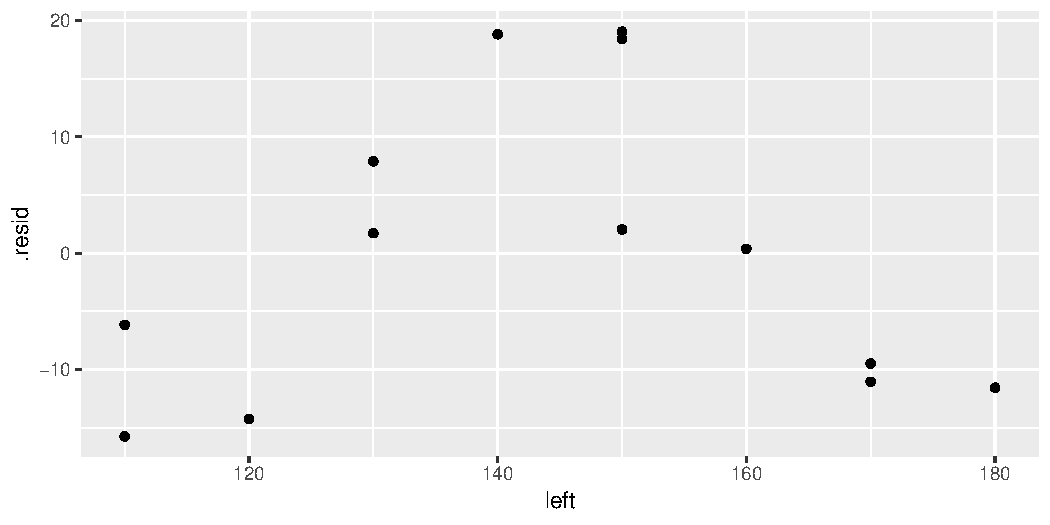
\includegraphics{figure/basingstoke-1.pdf}
\caption{plot of chunk basingstoke}
\end{figure}

\end{frame}

\begin{frame}[fragile]{Comments}
\protect\hypertarget{comments-8}{}

\begin{itemize}
\item
  There is a \emph{curved} relationship with \texttt{left}.
\item
  We should add \texttt{left}-squared to the regression (and therefore
  put \texttt{left} back in when we do that):
\end{itemize}

\begin{Shaded}
\begin{Highlighting}[]
\NormalTok{punting}\FloatTok{.3}\NormalTok{ <-}\StringTok{ }\KeywordTok{lm}\NormalTok{(punt }\OperatorTok{~}\StringTok{ }\NormalTok{left }\OperatorTok{+}\StringTok{ }\KeywordTok{I}\NormalTok{(left}\OperatorTok{^}\DecValTok{2}\NormalTok{) }\OperatorTok{+}\StringTok{ }\NormalTok{right,}
  \DataTypeTok{data =}\NormalTok{ punting}
\NormalTok{)}
\end{Highlighting}
\end{Shaded}

\end{frame}

\begin{frame}[fragile]{Regression with \texttt{left-squared}}
\protect\hypertarget{regression-with-left-squared}{}

\scriptsize

\begin{Shaded}
\begin{Highlighting}[]
\KeywordTok{summary}\NormalTok{(punting}\FloatTok{.3}\NormalTok{)}
\end{Highlighting}
\end{Shaded}

\begin{verbatim}
## 
## Call:
## lm(formula = punt ~ left + I(left^2) + right, data = punting)
## 
## Residuals:
##      Min       1Q   Median       3Q      Max 
## -11.3777  -5.3599   0.0459   4.5088  13.2669 
## 
## Coefficients:
##               Estimate Std. Error t value Pr(>|t|)   
## (Intercept) -4.623e+02  9.902e+01  -4.669  0.00117 **
## left         6.888e+00  1.462e+00   4.710  0.00110 **
## I(left^2)   -2.302e-02  4.927e-03  -4.672  0.00117 **
## right        7.396e-01  2.292e-01   3.227  0.01038 * 
## ---
## Signif. codes:  
## 0 '***' 0.001 '**' 0.01 '*' 0.05 '.' 0.1 ' ' 1
## 
## Residual standard error: 7.931 on 9 degrees of freedom
## Multiple R-squared:  0.9352, Adjusted R-squared:  0.9136 
## F-statistic:  43.3 on 3 and 9 DF,  p-value: 1.13e-05
\end{verbatim}

\normalsize

\end{frame}

\begin{frame}[fragile]{Comments}
\protect\hypertarget{comments-9}{}

\begin{itemize}
\item
  This was definitely a good idea (R-squared has clearly increased).
\item
  We would never have seen it without plotting residuals from
  \texttt{punting.2} (without \texttt{left}) against \texttt{left}.
\item
  Negative slope for \texttt{leftsq} means that increased left-leg
  strength only increases punting distance up to a point: beyond that,
  it decreases again.
\end{itemize}

\end{frame}

\hypertarget{logistic-regression-ordinalnominal-response}{%
\section{Logistic regression (ordinal/nominal
response)}\label{logistic-regression-ordinalnominal-response}}

\begin{frame}[fragile]{Logistic regression}
\protect\hypertarget{logistic-regression}{}

\begin{itemize}
\item
  When response variable is measured/counted, regression can work well.
\item
  But what if response is yes/no, lived/died, success/failure?
\item
  Model \emph{probability} of success.
\item
  Probability must be between 0 and 1; need method that ensures this.
\item
  \emph{Logistic regression} does this. In R, is a \emph{generalized
  linear model} with binomial ``family'':
\end{itemize}

\begin{Shaded}
\begin{Highlighting}[]
\KeywordTok{glm}\NormalTok{(y }\OperatorTok{~}\StringTok{ }\NormalTok{x, }\DataTypeTok{family=}\StringTok{"binomial"}\NormalTok{)}
\end{Highlighting}
\end{Shaded}

\begin{itemize}
\tightlist
\item
  Begin with simplest case.
\end{itemize}

\end{frame}

\begin{frame}[fragile]{Packages}
\protect\hypertarget{packages-1}{}

\begin{Shaded}
\begin{Highlighting}[]
\KeywordTok{library}\NormalTok{(MASS)}
\KeywordTok{library}\NormalTok{(tidyverse)}
\KeywordTok{library}\NormalTok{(broom)}
\KeywordTok{library}\NormalTok{(nnet)}
\end{Highlighting}
\end{Shaded}

\end{frame}

\begin{frame}[fragile]{The rats, part 1}
\protect\hypertarget{the-rats-part-1}{}

\begin{itemize}
\tightlist
\item
  Rats given dose of some poison; either live or die:
\end{itemize}

\small

\begin{verbatim}
dose status
0 lived
1 died
2 lived
3 lived
4 died
5 died
\end{verbatim}

\normalsize

\end{frame}

\begin{frame}[fragile]{Read in:}
\protect\hypertarget{read-in}{}

\begin{Shaded}
\begin{Highlighting}[]
\NormalTok{my_url <-}\StringTok{ "http://www.utsc.utoronto.ca/~butler/d29/rat.txt"}
\NormalTok{rats <-}\StringTok{ }\KeywordTok{read_delim}\NormalTok{(my_url, }\StringTok{" "}\NormalTok{)}
\end{Highlighting}
\end{Shaded}

\begin{verbatim}
## Parsed with column specification:
## cols(
##   dose = col_double(),
##   status = col_character()
## )
\end{verbatim}

\begin{Shaded}
\begin{Highlighting}[]
\KeywordTok{glimpse}\NormalTok{(rats)}
\end{Highlighting}
\end{Shaded}

\begin{verbatim}
## Observations: 6
## Variables: 2
## $ dose   <dbl> 0, 1, 2, 3, 4, 5
## $ status <chr> "lived", "died", "lived", "lived", "died",…
\end{verbatim}

\end{frame}

\begin{frame}[fragile]{Basic logistic regression}
\protect\hypertarget{basic-logistic-regression}{}

\begin{itemize}
\tightlist
\item
  Make response into a factor first:
\end{itemize}

\small

\begin{Shaded}
\begin{Highlighting}[]
\NormalTok{rats2 <-}\StringTok{ }\NormalTok{rats }\OperatorTok\StringTok{ }\KeywordTok{mutate}\NormalTok{(}\DataTypeTok{status =} \KeywordTok{factor}\NormalTok{(status))}
\end{Highlighting}
\end{Shaded}

\normalsize

\begin{itemize}
\tightlist
\item
  then fit model:
\end{itemize}

\small

\begin{Shaded}
\begin{Highlighting}[]
\NormalTok{status}\FloatTok{.1}\NormalTok{ <-}\StringTok{ }\KeywordTok{glm}\NormalTok{(status }\OperatorTok{~}\StringTok{ }\NormalTok{dose, }\DataTypeTok{family =} \StringTok{"binomial"}\NormalTok{, }\DataTypeTok{data =}\NormalTok{ rats2)}
\end{Highlighting}
\end{Shaded}

\normalsize

\end{frame}

\begin{frame}[fragile]{Output}
\protect\hypertarget{output-1}{}

\scriptsize

\begin{Shaded}
\begin{Highlighting}[]
\KeywordTok{summary}\NormalTok{(status}\FloatTok{.1}\NormalTok{)}
\end{Highlighting}
\end{Shaded}

\begin{verbatim}
## 
## Call:
## glm(formula = status ~ dose, family = "binomial", data = rats2)
## 
## Deviance Residuals: 
##       1        2        3        4        5        6  
##  0.5835  -1.6254   1.0381   1.3234  -0.7880  -0.5835  
## 
## Coefficients:
##             Estimate Std. Error z value Pr(>|z|)
## (Intercept)   1.6841     1.7979   0.937    0.349
## dose         -0.6736     0.6140  -1.097    0.273
## 
## (Dispersion parameter for binomial family taken to be 1)
## 
##     Null deviance: 8.3178  on 5  degrees of freedom
## Residual deviance: 6.7728  on 4  degrees of freedom
## AIC: 10.773
## 
## Number of Fisher Scoring iterations: 4
\end{verbatim}

\normalsize

\end{frame}

\begin{frame}{Interpreting the output}
\protect\hypertarget{interpreting-the-output}{}

\begin{itemize}
\item
  Like (multiple) regression, get tests of significance of individual
  \(x\)'s
\item
  Here not significant (only 6 observations).
\item
  ``Slope'' for dose is negative, meaning that as dose increases,
  probability of event modelled (survival) decreases.
\end{itemize}

\end{frame}

\begin{frame}[fragile]{Output part 2: predicted survival probs}
\protect\hypertarget{output-part-2-predicted-survival-probs}{}

\begin{Shaded}
\begin{Highlighting}[]
\NormalTok{p <-}\StringTok{ }\KeywordTok{predict}\NormalTok{(status}\FloatTok{.1}\NormalTok{, }\DataTypeTok{type =} \StringTok{"response"}\NormalTok{)}
\KeywordTok{cbind}\NormalTok{(rats, p)}
\end{Highlighting}
\end{Shaded}

\begin{verbatim}
##   dose status         p
## 1    0  lived 0.8434490
## 2    1   died 0.7331122
## 3    2  lived 0.5834187
## 4    3  lived 0.4165813
## 5    4   died 0.2668878
## 6    5   died 0.1565510
\end{verbatim}

\end{frame}

\begin{frame}[fragile]{The rats, more}
\protect\hypertarget{the-rats-more}{}

\begin{itemize}
\item
  More realistic: more rats at each dose (say 10).
\item
  Listing each rat on one line makes a big data file.
\item
  Use format below: dose, number of survivals, number of deaths.
\end{itemize}

\begin{verbatim}

dose lived died
0    10    0
1     7    3 
2     6    4 
3     4    6 
4     2    8 
5     1    9  
\end{verbatim}

\begin{itemize}
\item
  6 lines of data correspond to 60 actual rats.
\item
  Saved in \texttt{rat2.txt}.
\end{itemize}

\end{frame}

\begin{frame}[fragile]{These data}
\protect\hypertarget{these-data}{}

\footnotesize

\begin{Shaded}
\begin{Highlighting}[]
\NormalTok{my_url <-}\StringTok{ "http://www.utsc.utoronto.ca/~butler/d29/rat2.txt"}
\NormalTok{rat2 <-}\StringTok{ }\KeywordTok{read_delim}\NormalTok{(my_url, }\StringTok{" "}\NormalTok{)}
\end{Highlighting}
\end{Shaded}

\begin{verbatim}
## Parsed with column specification:
## cols(
##   dose = col_double(),
##   lived = col_double(),
##   died = col_double()
## )
\end{verbatim}

\begin{Shaded}
\begin{Highlighting}[]
\NormalTok{rat2}
\end{Highlighting}
\end{Shaded}

\begin{verbatim}
## # A tibble: 6 x 3
##    dose lived  died
##   <dbl> <dbl> <dbl>
## 1     0    10     0
## 2     1     7     3
## 3     2     6     4
## 4     3     4     6
## 5     4     2     8
## 6     5     1     9
\end{verbatim}

\normalsize

\end{frame}

\begin{frame}[fragile]{Create response matrix:}
\protect\hypertarget{create-response-matrix}{}

\begin{itemize}
\tightlist
\item
  Each row contains \emph{multiple} observations.
\item
  Create \emph{two-column} response:

  \begin{itemize}
  \tightlist
  \item
    \#survivals in first column,
  \item
    \#deaths in second.
  \end{itemize}
\end{itemize}

\footnotesize

\begin{Shaded}
\begin{Highlighting}[]
\NormalTok{response <-}\StringTok{ }\KeywordTok{with}\NormalTok{(rat2, }\KeywordTok{cbind}\NormalTok{(lived, died))}
\NormalTok{response}
\end{Highlighting}
\end{Shaded}

\begin{verbatim}
##      lived died
## [1,]    10    0
## [2,]     7    3
## [3,]     6    4
## [4,]     4    6
## [5,]     2    8
## [6,]     1    9
\end{verbatim}

\normalsize

\begin{itemize}
\tightlist
\item
  Response is R \texttt{matrix}:
\end{itemize}

\footnotesize

\begin{Shaded}
\begin{Highlighting}[]
\KeywordTok{class}\NormalTok{(response)}
\end{Highlighting}
\end{Shaded}

\begin{verbatim}
## [1] "matrix"
\end{verbatim}

\normalsize

\end{frame}

\begin{frame}[fragile]{Fit logistic regression}
\protect\hypertarget{fit-logistic-regression}{}

\begin{itemize}
\tightlist
\item
  using response you just made:
\end{itemize}

\begin{Shaded}
\begin{Highlighting}[]
\NormalTok{rat2}\FloatTok{.1}\NormalTok{ <-}\StringTok{ }\KeywordTok{glm}\NormalTok{(response }\OperatorTok{~}\StringTok{ }\NormalTok{dose,}
  \DataTypeTok{family =} \StringTok{"binomial"}\NormalTok{,}
  \DataTypeTok{data =}\NormalTok{ rat2}
\NormalTok{)}
\end{Highlighting}
\end{Shaded}

\end{frame}

\begin{frame}[fragile]{Output}
\protect\hypertarget{output-2}{}

\scriptsize

\begin{Shaded}
\begin{Highlighting}[]
\KeywordTok{summary}\NormalTok{(rat2}\FloatTok{.1}\NormalTok{)}
\end{Highlighting}
\end{Shaded}

\begin{verbatim}
## 
## Call:
## glm(formula = response ~ dose, family = "binomial", data = rat2)
## 
## Deviance Residuals: 
##       1        2        3        4        5        6  
##  1.3421  -0.7916  -0.1034   0.1034   0.0389   0.1529  
## 
## Coefficients:
##             Estimate Std. Error z value Pr(>|z|)    
## (Intercept)   2.3619     0.6719   3.515 0.000439 ***
## dose         -0.9448     0.2351  -4.018 5.87e-05 ***
## ---
## Signif. codes:  
## 0 '***' 0.001 '**' 0.01 '*' 0.05 '.' 0.1 ' ' 1
## 
## (Dispersion parameter for binomial family taken to be 1)
## 
##     Null deviance: 27.530  on 5  degrees of freedom
## Residual deviance:  2.474  on 4  degrees of freedom
## AIC: 18.94
## 
## Number of Fisher Scoring iterations: 4
\end{verbatim}

\normalsize

\end{frame}

\begin{frame}[fragile]{Predicted survival probs}
\protect\hypertarget{predicted-survival-probs}{}

\begin{Shaded}
\begin{Highlighting}[]
\NormalTok{p <-}\StringTok{ }\KeywordTok{predict}\NormalTok{(rat2}\FloatTok{.1}\NormalTok{, }\DataTypeTok{type =} \StringTok{"response"}\NormalTok{)}
\KeywordTok{cbind}\NormalTok{(rat2, p)}
\end{Highlighting}
\end{Shaded}

\begin{verbatim}
##   dose lived died         p
## 1    0    10    0 0.9138762
## 2    1     7    3 0.8048905
## 3    2     6    4 0.6159474
## 4    3     4    6 0.3840526
## 5    4     2    8 0.1951095
## 6    5     1    9 0.0861238
\end{verbatim}

\end{frame}

\begin{frame}{Comments}
\protect\hypertarget{comments-10}{}

\begin{itemize}
\item
  Significant effect of dose.
\item
  Effect of larger dose is to \emph{decrease} survival probability
  (``slope'' negative; also see in decreasing predictions.)
\end{itemize}

\end{frame}

\begin{frame}{Multiple logistic regression}
\protect\hypertarget{multiple-logistic-regression}{}

\begin{itemize}
\item
  With more than one \(x\), works much like multiple regression.
\item
  Example: study of patients with blood poisoning severe enough to
  warrant surgery. Relate survival to other potential risk factors.
\item
  Variables, 1=present, 0=absent:

  \begin{itemize}
  \tightlist
  \item
    survival (death from sepsis=1), response
  \item
    shock
  \item
    malnutrition
  \item
    alcoholism
  \item
    age (as numerical variable)
  \item
    bowel infarction
  \end{itemize}
\item
  See what relates to death.
\end{itemize}

\end{frame}

\begin{frame}[fragile]{Read in data}
\protect\hypertarget{read-in-data}{}

\begin{Shaded}
\begin{Highlighting}[]
\NormalTok{my_url <-}\StringTok{ }
\StringTok{  "http://www.utsc.utoronto.ca/~butler/d29/sepsis.txt"}
\NormalTok{sepsis <-}\StringTok{ }\KeywordTok{read_delim}\NormalTok{(my_url, }\StringTok{" "}\NormalTok{)}
\end{Highlighting}
\end{Shaded}

\begin{verbatim}
## Parsed with column specification:
## cols(
##   death = col_double(),
##   shock = col_double(),
##   malnut = col_double(),
##   alcohol = col_double(),
##   age = col_double(),
##   bowelinf = col_double()
## )
\end{verbatim}

\end{frame}

\begin{frame}[fragile]{The data}
\protect\hypertarget{the-data-2}{}

\begin{Shaded}
\begin{Highlighting}[]
\NormalTok{sepsis}
\end{Highlighting}
\end{Shaded}

\begin{verbatim}
## # A tibble: 106 x 6
##    death shock malnut alcohol   age bowelinf
##    <dbl> <dbl>  <dbl>   <dbl> <dbl>    <dbl>
##  1     0     0      0       0    56        0
##  2     0     0      0       0    80        0
##  3     0     0      0       0    61        0
##  4     0     0      0       0    26        0
##  5     0     0      0       0    53        0
##  6     1     0      1       0    87        0
##  7     0     0      0       0    21        0
##  8     1     0      0       1    69        0
##  9     0     0      0       0    57        0
## 10     0     0      1       0    76        0
## # … with 96 more rows
\end{verbatim}

\end{frame}

\begin{frame}[fragile]{Fit model}
\protect\hypertarget{fit-model}{}

\begin{Shaded}
\begin{Highlighting}[]
\NormalTok{sepsis}\FloatTok{.1}\NormalTok{ <-}\StringTok{ }\KeywordTok{glm}\NormalTok{(death }\OperatorTok{~}\StringTok{ }\NormalTok{shock }\OperatorTok{+}\StringTok{ }\NormalTok{malnut }\OperatorTok{+}\StringTok{ }\NormalTok{alcohol }\OperatorTok{+}\StringTok{ }\NormalTok{age }\OperatorTok{+}
\StringTok{  }\NormalTok{bowelinf,}
\DataTypeTok{family =} \StringTok{"binomial"}\NormalTok{,}
\DataTypeTok{data =}\NormalTok{ sepsis}
\NormalTok{)}
\end{Highlighting}
\end{Shaded}

\end{frame}

\begin{frame}[fragile]{Output part 1}
\protect\hypertarget{output-part-1}{}

\begin{Shaded}
\begin{Highlighting}[]
\KeywordTok{tidy}\NormalTok{(sepsis}\FloatTok{.1}\NormalTok{)}
\end{Highlighting}
\end{Shaded}

\begin{verbatim}
## # A tibble: 6 x 5
##   term        estimate std.error statistic  p.value
##   <chr>          <dbl>     <dbl>     <dbl>    <dbl>
## 1 (Intercept)  -9.75      2.54       -3.84 0.000124
## 2 shock         3.67      1.16        3.15 0.00161 
## 3 malnut        1.22      0.728       1.67 0.0948  
## 4 alcohol       3.35      0.982       3.42 0.000635
## 5 age           0.0922    0.0303      3.04 0.00237 
## 6 bowelinf      2.80      1.16        2.40 0.0162
\end{verbatim}

\begin{itemize}
\item
  All P-values fairly small
\item
  but \texttt{malnut} not significant: remove.
\end{itemize}

\end{frame}

\begin{frame}[fragile]{Removing \texttt{malnut}}
\protect\hypertarget{removing-malnut}{}

\begin{Shaded}
\begin{Highlighting}[]
\NormalTok{sepsis}\FloatTok{.2}\NormalTok{ <-}\StringTok{ }\KeywordTok{update}\NormalTok{(sepsis}\FloatTok{.1}\NormalTok{, . }\OperatorTok{~}\StringTok{ }\NormalTok{. }\OperatorTok{-}\StringTok{ }\NormalTok{malnut)}
\KeywordTok{tidy}\NormalTok{(sepsis}\FloatTok{.2}\NormalTok{)}
\end{Highlighting}
\end{Shaded}

\begin{verbatim}
## # A tibble: 5 x 5
##   term        estimate std.error statistic  p.value
##   <chr>          <dbl>     <dbl>     <dbl>    <dbl>
## 1 (Intercept)  -8.89      2.32       -3.84 0.000124
## 2 shock         3.70      1.10        3.35 0.000797
## 3 alcohol       3.19      0.917       3.47 0.000514
## 4 age           0.0898    0.0292      3.07 0.00211 
## 5 bowelinf      2.39      1.07        2.23 0.0260
\end{verbatim}

\begin{itemize}
\tightlist
\item
  Everything significant now.
\end{itemize}

\end{frame}

\begin{frame}[fragile]{Comments}
\protect\hypertarget{comments-11}{}

\begin{itemize}
\item
  Most of the original \(x\)'s helped predict death. Only
  \texttt{malnut} seemed not to add anything.
\item
  Removed \texttt{malnut} and tried again.
\item
  Everything remaining is significant (though \texttt{bowelinf} actually
  became \emph{less} significant).
\item
  All coefficients are \emph{positive}, so having any of the risk
  factors (or being older) \emph{increases} risk of death.
\end{itemize}

\end{frame}

\begin{frame}[fragile]{Predictions from model without ``malnut''}
\protect\hypertarget{predictions-from-model-without-malnut}{}

\begin{itemize}
\tightlist
\item
  A few chosen at random:
\end{itemize}

\normalsize

\begin{Shaded}
\begin{Highlighting}[]
\NormalTok{sepsis.pred <-}\StringTok{ }\KeywordTok{predict}\NormalTok{(sepsis}\FloatTok{.2}\NormalTok{, }\DataTypeTok{type =} \StringTok{"response"}\NormalTok{)}
\NormalTok{d <-}\StringTok{ }\KeywordTok{data.frame}\NormalTok{(sepsis, sepsis.pred)}
\NormalTok{myrows <-}\StringTok{ }\KeywordTok{c}\NormalTok{(}\DecValTok{4}\NormalTok{, }\DecValTok{1}\NormalTok{, }\DecValTok{2}\NormalTok{, }\DecValTok{11}\NormalTok{, }\DecValTok{32}\NormalTok{)}
\KeywordTok{slice}\NormalTok{(d, myrows)}
\end{Highlighting}
\end{Shaded}

\begin{verbatim}
##   death shock malnut alcohol age bowelinf sepsis.pred
## 1     0     0      0       0  26        0 0.001415347
## 2     0     0      0       0  56        0 0.020552383
## 3     0     0      0       0  80        0 0.153416834
## 4     1     0      0       1  66        1 0.931290137
## 5     1     0      0       1  49        0 0.213000997
\end{verbatim}

\normalsize

\end{frame}

\begin{frame}{Comments}
\protect\hypertarget{comments-12}{}

\begin{itemize}
\item
  Survival chances pretty good if no risk factors, though decreasing
  with age.
\item
  Having more than one risk factor reduces survival chances
  dramatically.
\item
  Usually good job of predicting survival; sometimes death predicted to
  survive.
\end{itemize}

\end{frame}

\begin{frame}{Assessing proportionality of odds for age}
\protect\hypertarget{assessing-proportionality-of-odds-for-age}{}

\begin{itemize}
\item
  An assumption we made is that log-odds of survival depends linearly on
  age.
\item
  Hard to get your head around, but basic idea is that survival chances
  go continuously up (or down) with age, instead of (for example) going
  up and then down.
\item
  In this case, seems reasonable, but should check:
\end{itemize}

\end{frame}

\begin{frame}[fragile]{Residuals vs.~age}
\protect\hypertarget{residuals-vs.age}{}

\begin{Shaded}
\begin{Highlighting}[]
\KeywordTok{ggplot}\NormalTok{(}\KeywordTok{augment}\NormalTok{(sepsis}\FloatTok{.2}\NormalTok{), }\KeywordTok{aes}\NormalTok{(}\DataTypeTok{x =}\NormalTok{ age, }\DataTypeTok{y =}\NormalTok{ .resid)) }\OperatorTok{+}
\StringTok{  }\KeywordTok{geom_point}\NormalTok{()}
\end{Highlighting}
\end{Shaded}

\begin{figure}
\centering
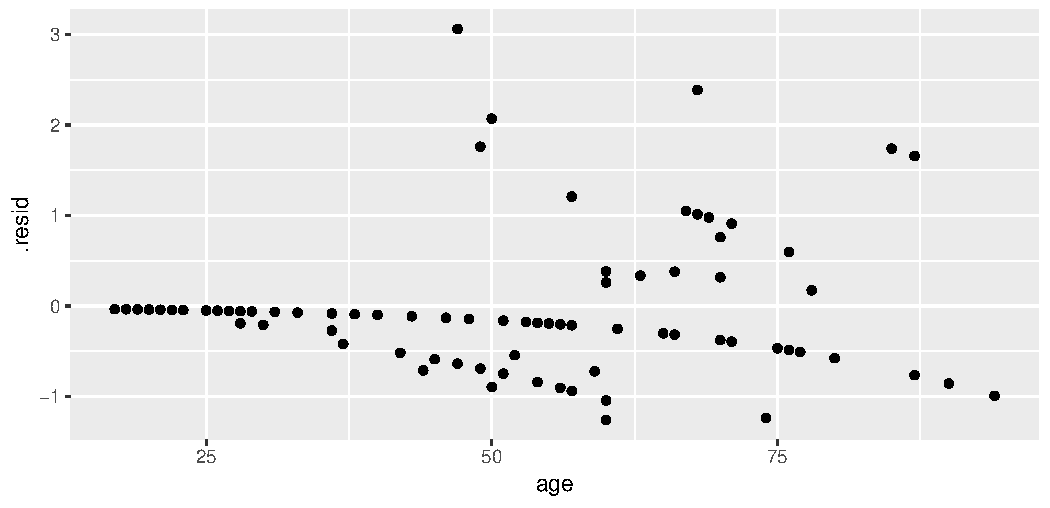
\includegraphics{figure/virtusentella-1.pdf}
\caption{plot of chunk virtusentella}
\end{figure}

\end{frame}

\begin{frame}{Comments}
\protect\hypertarget{comments-13}{}

\begin{itemize}
\item
  No apparent problems overall.
\item
  Confusing ``line'' across: no risk factors, survived.
\end{itemize}

\end{frame}

\begin{frame}{Probability and odds}
\protect\hypertarget{probability-and-odds}{}

\begin{itemize}
\item
  For probability \(p\), odds is \(p/(1-p)\):

  \begin{tabular}{rrrl}
      \hline
      Prob.\ & Odds & log-odds & in words\\
      \hline
      0.5 & $0.5/0.5=1/1=1.00$ & $0.00$ &  ``even money''\\
      0.1 & $0.1/0.9=1/9=0.11$ & $-2.20$ & ``9 to 1''\\
      0.4 & $0.4/0.6=1/1.5=0.67$ & $-0.41$ & ``1.5 to 1''\\
      0.8 & $0.8/0.2=4/1=4.00$ & $1.39$ & ``4 to 1 on''\\
      \hline
    \end{tabular}
\item
  Gamblers use odds: if you win at 9 to 1 odds, get original stake back
  plus 9 times the stake.
\item
  Probability has to be between 0 and 1
\item
  Odds between 0 and infinity
\item
  \emph{Log}-odds can be anything: any log-odds corresponds to valid
  probability.
\end{itemize}

\end{frame}

\begin{frame}{Odds ratio}
\protect\hypertarget{odds-ratio}{}

\begin{itemize}
\item
  Suppose 90 of 100 men drank wine last week, but only 20 of 100 women.
\item
  Prob of man drinking wine \(90/100=0.9\), woman \(20/100=0.2\).
\item
  Odds of man drinking wine \(0.9/0.1=9\), woman \(0.2/0.8=0.25\).
\item
  Ratio of odds is \(9/0.25=36\).
\item
  Way of quantifying difference between men and women: ``odds of
  drinking wine 36 times larger for males than females''.
\end{itemize}

\end{frame}

\begin{frame}[fragile]{Sepsis data again}
\protect\hypertarget{sepsis-data-again}{}

\begin{itemize}
\tightlist
\item
  Recall prediction of probability of death from risk factors:
\end{itemize}

\begin{Shaded}
\begin{Highlighting}[]
\NormalTok{sepsis.}\FloatTok{2.}\NormalTok{tidy <-}\StringTok{ }\KeywordTok{tidy}\NormalTok{(sepsis}\FloatTok{.2}\NormalTok{)}
\NormalTok{sepsis.}\FloatTok{2.}\NormalTok{tidy}
\end{Highlighting}
\end{Shaded}

\begin{verbatim}
## # A tibble: 5 x 5
##   term        estimate std.error statistic  p.value
##   <chr>          <dbl>     <dbl>     <dbl>    <dbl>
## 1 (Intercept)  -8.89      2.32       -3.84 0.000124
## 2 shock         3.70      1.10        3.35 0.000797
## 3 alcohol       3.19      0.917       3.47 0.000514
## 4 age           0.0898    0.0292      3.07 0.00211 
## 5 bowelinf      2.39      1.07        2.23 0.0260
\end{verbatim}

\begin{itemize}
\tightlist
\item
  Slopes in column \texttt{estimate}.
\end{itemize}

\end{frame}

\begin{frame}[fragile]{Multiplying the odds}
\protect\hypertarget{multiplying-the-odds}{}

\begin{itemize}
\tightlist
\item
  Can interpret slopes by taking ``exp'' of them. We ignore intercept.
\end{itemize}

\begin{Shaded}
\begin{Highlighting}[]
\NormalTok{sepsis.}\FloatTok{2.}\NormalTok{tidy }\OperatorTok\StringTok{ }
\StringTok{  }\KeywordTok{mutate}\NormalTok{(}\DataTypeTok{exp_coeff=}\KeywordTok{exp}\NormalTok{(estimate)) }\OperatorTok\StringTok{ }
\StringTok{  }\KeywordTok{select}\NormalTok{(term, exp_coeff)}
\end{Highlighting}
\end{Shaded}

\begin{verbatim}
## # A tibble: 5 x 2
##   term        exp_coeff
##   <chr>           <dbl>
## 1 (Intercept)  0.000137
## 2 shock       40.5     
## 3 alcohol     24.2     
## 4 age          1.09    
## 5 bowelinf    10.9
\end{verbatim}

\end{frame}

\begin{frame}[fragile]{Interpretation}
\protect\hypertarget{interpretation}{}

\small

\begin{verbatim}
## # A tibble: 5 x 2
##   term        exp_coeff
##   <chr>           <dbl>
## 1 (Intercept)  0.000137
## 2 shock       40.5     
## 3 alcohol     24.2     
## 4 age          1.09    
## 5 bowelinf    10.9
\end{verbatim}

\normalsize

\begin{itemize}
\item
  These say ``how much do you \emph{multiply} odds of death by for
  increase of 1 in corresponding risk factor?'' Or, what is odds ratio
  for that factor being 1 (present) vs.~0 (absent)?
\item
  Eg.~being alcoholic vs.~not increases odds of death by 24 times
\item
  One year older multiplies odds by about 1.1 times. Over 40 years,
  about \(1.09^{40}=31\) times.
\end{itemize}

\end{frame}

\begin{frame}{Odds ratio and relative risk}
\protect\hypertarget{odds-ratio-and-relative-risk}{}

\begin{itemize}
\item
  \textbf{Relative risk} is ratio of probabilities.
\item
  Above: 90 of 100 men (0.9) drank wine, 20 of 100 women (0.2).
\item
  Relative risk 0.9/0.2=4.5. (odds ratio was 36).
\item
  When probabilities small, relative risk and odds ratio similar.
\item
  Eg.~prob of man having disease 0.02, woman 0.01.
\item
  Relative risk \(0.02/0.01=2\).
\end{itemize}

\end{frame}

\begin{frame}[fragile]{Odds ratio vs.~relative risk}
\protect\hypertarget{odds-ratio-vs.relative-risk}{}

\begin{itemize}
\tightlist
\item
  Odds for men and for women:
\end{itemize}

\begin{Shaded}
\begin{Highlighting}[]
\NormalTok{(od1 <-}\StringTok{ }\FloatTok{0.02} \OperatorTok{/}\StringTok{ }\FloatTok{0.98}\NormalTok{) }\CommentTok{# men}
\end{Highlighting}
\end{Shaded}

\begin{verbatim}
## [1] 0.02040816
\end{verbatim}

\begin{Shaded}
\begin{Highlighting}[]
\NormalTok{(od2 <-}\StringTok{ }\FloatTok{0.01} \OperatorTok{/}\StringTok{ }\FloatTok{0.99}\NormalTok{) }\CommentTok{# women}
\end{Highlighting}
\end{Shaded}

\begin{verbatim}
## [1] 0.01010101
\end{verbatim}

\begin{itemize}
\tightlist
\item
  Odds ratio
\end{itemize}

\begin{Shaded}
\begin{Highlighting}[]
\NormalTok{od1 }\OperatorTok{/}\StringTok{ }\NormalTok{od2}
\end{Highlighting}
\end{Shaded}

\begin{verbatim}
## [1] 2.020408
\end{verbatim}

\begin{itemize}
\tightlist
\item
  Very close to relative risk of 2.
\end{itemize}

\end{frame}

\begin{frame}{More than 2 response categories}
\protect\hypertarget{more-than-2-response-categories}{}

\begin{itemize}
\item
  With 2 response categories, model the probability of one, and prob of
  other is one minus that. So doesn't matter which category you model.
\item
  With more than 2 categories, have to think more carefully about the
  categories: are they
\item
  \emph{ordered}: you can put them in a natural order (like low, medium,
  high)
\item
  \emph{nominal}: ordering the categories doesn't make sense (like red,
  green, blue).
\item
  R handles both kinds of response; learn how.
\end{itemize}

\end{frame}

\begin{frame}{Ordinal response: the miners}
\protect\hypertarget{ordinal-response-the-miners}{}

\begin{itemize}
\item
  Model probability of being in given category \emph{or lower}.
\item
  Example: coal-miners often suffer disease pneumoconiosis. Likelihood
  of disease believed to be greater among miners who have worked longer.
\item
  Severity of disease measured on categorical scale: none, moderate, 3
  severe.
\end{itemize}

\end{frame}

\begin{frame}[fragile]{Miners data}
\protect\hypertarget{miners-data}{}

\begin{itemize}
\tightlist
\item
  Data are frequencies:
\end{itemize}

\begin{verbatim}
Exposure None Moderate Severe
5.8       98      0       0
15.0      51      2       1
21.5      34      6       3
27.5      35      5       8
33.5      32     10       9
39.5      23      7       8
46.0      12      6      10
51.5       4      2       5
\end{verbatim}

\end{frame}

\begin{frame}[fragile]{Reading the data}
\protect\hypertarget{reading-the-data}{}

Data in aligned columns with more than one space between, so:

\small

\begin{Shaded}
\begin{Highlighting}[]
\NormalTok{my_url <-}\StringTok{ "http://www.utsc.utoronto.ca/~butler/d29/miners-tab.txt"}
\NormalTok{freqs <-}\StringTok{ }\KeywordTok{read_table}\NormalTok{(my_url)}
\end{Highlighting}
\end{Shaded}

\begin{verbatim}
## Parsed with column specification:
## cols(
##   Exposure = col_double(),
##   None = col_double(),
##   Moderate = col_double(),
##   Severe = col_double()
## )
\end{verbatim}

\normalsize

\end{frame}

\begin{frame}[fragile]{The data}
\protect\hypertarget{the-data-3}{}

\begin{Shaded}
\begin{Highlighting}[]
\NormalTok{freqs}
\end{Highlighting}
\end{Shaded}

\begin{verbatim}
## # A tibble: 8 x 4
##   Exposure  None Moderate Severe
##      <dbl> <dbl>    <dbl>  <dbl>
## 1      5.8    98        0      0
## 2     15      51        2      1
## 3     21.5    34        6      3
## 4     27.5    35        5      8
## 5     33.5    32       10      9
## 6     39.5    23        7      8
## 7     46      12        6     10
## 8     51.5     4        2      5
\end{verbatim}

\end{frame}

\begin{frame}[fragile]{Tidying and row proportions}
\protect\hypertarget{tidying-and-row-proportions}{}

\begin{Shaded}
\begin{Highlighting}[]
\NormalTok{freqs }\OperatorTok
\StringTok{  }\KeywordTok{gather}\NormalTok{(Severity, Freq, None}\OperatorTok{:}\NormalTok{Severe) }\OperatorTok
\StringTok{  }\KeywordTok{group_by}\NormalTok{(Exposure) }\OperatorTok
\StringTok{  }\KeywordTok{mutate}\NormalTok{(}\DataTypeTok{proportion =}\NormalTok{ Freq }\OperatorTok{/}\StringTok{ }\KeywordTok{sum}\NormalTok{(Freq)) ->}\StringTok{ }\NormalTok{miners}
\end{Highlighting}
\end{Shaded}

\end{frame}

\begin{frame}[fragile]{Result}
\protect\hypertarget{result}{}

\small

\begin{Shaded}
\begin{Highlighting}[]
\NormalTok{miners}
\end{Highlighting}
\end{Shaded}

\begin{verbatim}
## # A tibble: 24 x 4
## # Groups:   Exposure [8]
##    Exposure Severity  Freq proportion
##       <dbl> <chr>    <dbl>      <dbl>
##  1      5.8 None        98     1     
##  2     15   None        51     0.944 
##  3     21.5 None        34     0.791 
##  4     27.5 None        35     0.729 
##  5     33.5 None        32     0.627 
##  6     39.5 None        23     0.605 
##  7     46   None        12     0.429 
##  8     51.5 None         4     0.364 
##  9      5.8 Moderate     0     0     
## 10     15   Moderate     2     0.0370
## # … with 14 more rows
\end{verbatim}

\normalsize

\end{frame}

\begin{frame}[fragile]{Plot proportions against exposure}
\protect\hypertarget{plot-proportions-against-exposure}{}

\small

\begin{Shaded}
\begin{Highlighting}[]
\KeywordTok{ggplot}\NormalTok{(miners, }\KeywordTok{aes}\NormalTok{(}\DataTypeTok{x =}\NormalTok{ Exposure, }\DataTypeTok{y =}\NormalTok{ proportion,}
                   \DataTypeTok{colour =}\NormalTok{ Severity)) }\OperatorTok{+}\StringTok{ }
\StringTok{  }\KeywordTok{geom_point}\NormalTok{() }\OperatorTok{+}\StringTok{ }\KeywordTok{geom_smooth}\NormalTok{(}\DataTypeTok{se =}\NormalTok{ F)}
\end{Highlighting}
\end{Shaded}

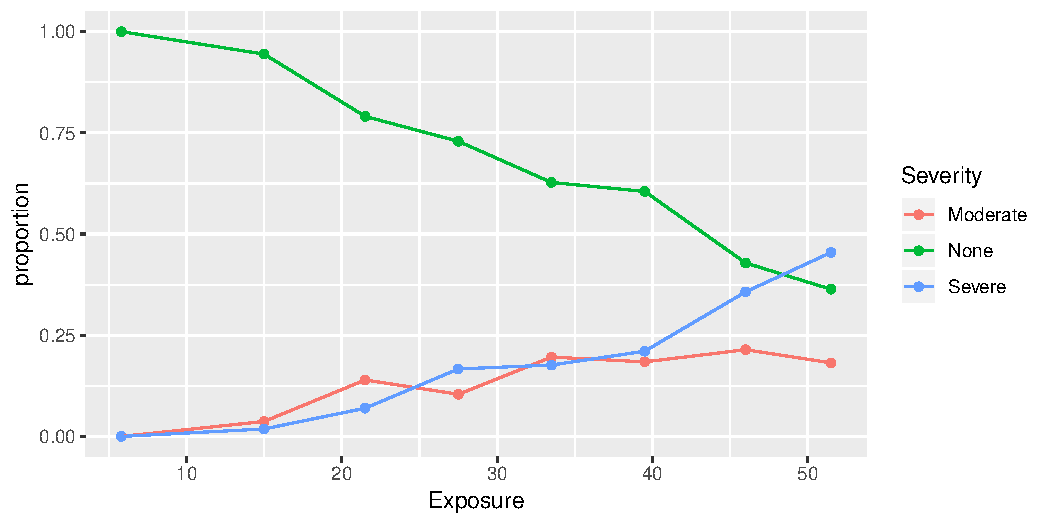
\includegraphics{figure/unnamed-chunk-85-1.pdf} \normalsize

\end{frame}

\begin{frame}[fragile]{Reminder of data setup}
\protect\hypertarget{reminder-of-data-setup}{}

\footnotesize

\begin{Shaded}
\begin{Highlighting}[]
\NormalTok{miners}
\end{Highlighting}
\end{Shaded}

\begin{verbatim}
## # A tibble: 24 x 4
## # Groups:   Exposure [8]
##    Exposure Severity  Freq proportion
##       <dbl> <chr>    <dbl>      <dbl>
##  1      5.8 None        98     1     
##  2     15   None        51     0.944 
##  3     21.5 None        34     0.791 
##  4     27.5 None        35     0.729 
##  5     33.5 None        32     0.627 
##  6     39.5 None        23     0.605 
##  7     46   None        12     0.429 
##  8     51.5 None         4     0.364 
##  9      5.8 Moderate     0     0     
## 10     15   Moderate     2     0.0370
## # … with 14 more rows
\end{verbatim}

\normalsize

\end{frame}

\begin{frame}[fragile]{Creating an ordered factor}
\protect\hypertarget{creating-an-ordered-factor}{}

\begin{itemize}
\item
  Problem: on plot, \texttt{Severity} categories in \emph{wrong
  order}.
\item
  \emph{In the data frame}, categories in \emph{correct} order.
\item
  Package \texttt{forcats} (in \texttt{tidyverse}) has functions for
  creating factors to specifications.
\item
  \texttt{fct\_inorder} takes levels \emph{in order they appear in
  data}:
\end{itemize}

\begin{Shaded}
\begin{Highlighting}[]
\NormalTok{miners }\OperatorTok
\StringTok{  }\KeywordTok{mutate}\NormalTok{(}\DataTypeTok{sev_ord =} \KeywordTok{fct_inorder}\NormalTok{(Severity)) ->}\StringTok{ }\NormalTok{miners}
\end{Highlighting}
\end{Shaded}

\begin{itemize}
\tightlist
\item
  To check:
\end{itemize}

\begin{Shaded}
\begin{Highlighting}[]
\KeywordTok{levels}\NormalTok{(miners}\OperatorTok{$}\NormalTok{sev_ord)}
\end{Highlighting}
\end{Shaded}

\begin{verbatim}
## [1] "None"     "Moderate" "Severe"
\end{verbatim}

\end{frame}

\begin{frame}[fragile]{New data frame}
\protect\hypertarget{new-data-frame}{}

\small

\begin{Shaded}
\begin{Highlighting}[]
\NormalTok{miners}
\end{Highlighting}
\end{Shaded}

\begin{verbatim}
## # A tibble: 24 x 5
## # Groups:   Exposure [8]
##    Exposure Severity  Freq proportion sev_ord 
##       <dbl> <chr>    <dbl>      <dbl> <fct>   
##  1      5.8 None        98     1      None    
##  2     15   None        51     0.944  None    
##  3     21.5 None        34     0.791  None    
##  4     27.5 None        35     0.729  None    
##  5     33.5 None        32     0.627  None    
##  6     39.5 None        23     0.605  None    
##  7     46   None        12     0.429  None    
##  8     51.5 None         4     0.364  None    
##  9      5.8 Moderate     0     0      Moderate
## 10     15   Moderate     2     0.0370 Moderate
## # … with 14 more rows
\end{verbatim}

\normalsize

\end{frame}

\begin{frame}[fragile]{Improved plot}
\protect\hypertarget{improved-plot}{}

\begin{Shaded}
\begin{Highlighting}[]
\KeywordTok{ggplot}\NormalTok{(miners, }\KeywordTok{aes}\NormalTok{(}\DataTypeTok{x =}\NormalTok{ Exposure, }\DataTypeTok{y =}\NormalTok{ proportion,}
                   \DataTypeTok{colour =}\NormalTok{ sev_ord)) }\OperatorTok{+}\StringTok{ }
\StringTok{  }\KeywordTok{geom_point}\NormalTok{() }\OperatorTok{+}\StringTok{ }\KeywordTok{geom_smooth}\NormalTok{(}\DataTypeTok{se =}\NormalTok{ F)}
\end{Highlighting}
\end{Shaded}

\begin{figure}
\centering
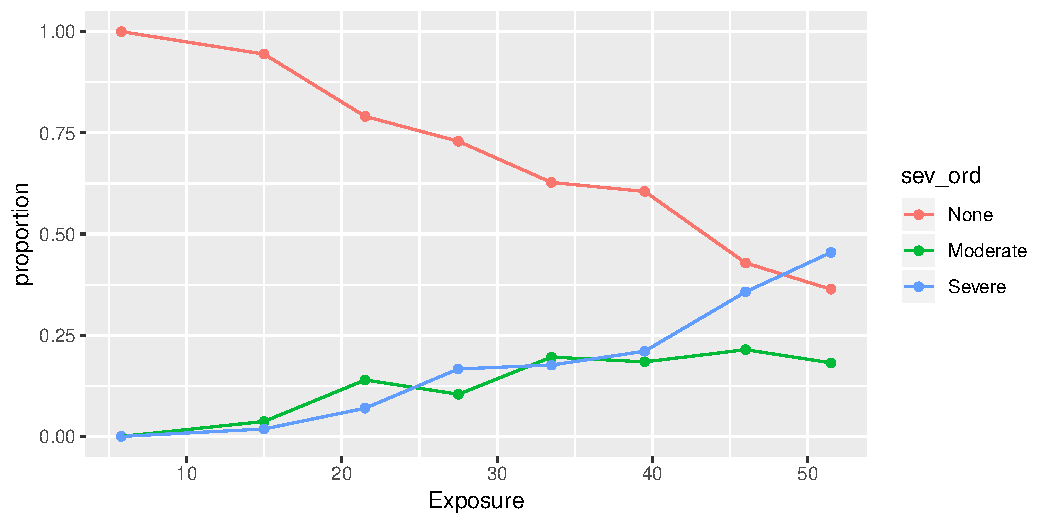
\includegraphics{figure/unnamed-chunk-90-1.pdf}
\caption{plot of chunk unnamed-chunk-90}
\end{figure}

\end{frame}

\begin{frame}[fragile]{Fitting ordered logistic model}
\protect\hypertarget{fitting-ordered-logistic-model}{}

Use function \texttt{polr} from package \texttt{MASS}. Like
\texttt{glm}.

\begin{Shaded}
\begin{Highlighting}[]
\NormalTok{sev}\FloatTok{.1}\NormalTok{ <-}\StringTok{ }\KeywordTok{polr}\NormalTok{(sev_ord }\OperatorTok{~}\StringTok{ }\NormalTok{Exposure,}
  \DataTypeTok{weights =}\NormalTok{ Freq,}
  \DataTypeTok{data =}\NormalTok{ miners}
\NormalTok{)}
\end{Highlighting}
\end{Shaded}

\end{frame}

\begin{frame}[fragile]{Output: not very illuminating}
\protect\hypertarget{output-not-very-illuminating}{}

\scriptsize

\begin{Shaded}
\begin{Highlighting}[]
\KeywordTok{summary}\NormalTok{(sev}\FloatTok{.1}\NormalTok{)}
\end{Highlighting}
\end{Shaded}

\begin{verbatim}
## 
## Re-fitting to get Hessian
\end{verbatim}

\begin{verbatim}
## Call:
## polr(formula = sev_ord ~ Exposure, data = miners, weights = Freq)
## 
## Coefficients:
##           Value Std. Error t value
## Exposure 0.0959    0.01194   8.034
## 
## Intercepts:
##                 Value   Std. Error t value
## None|Moderate    3.9558  0.4097     9.6558
## Moderate|Severe  4.8690  0.4411    11.0383
## 
## Residual Deviance: 416.9188 
## AIC: 422.9188
\end{verbatim}

\normalsize

\end{frame}

\begin{frame}[fragile]{Does exposure have an effect?}
\protect\hypertarget{does-exposure-have-an-effect}{}

Fit model without \texttt{Exposure}, and compare using \texttt{anova}.
Note \texttt{1} for model with just intercept:

\small

\begin{Shaded}
\begin{Highlighting}[]
\NormalTok{sev}\FloatTok{.0}\NormalTok{ <-}\StringTok{ }\KeywordTok{polr}\NormalTok{(sev_ord }\OperatorTok{~}\StringTok{ }\DecValTok{1}\NormalTok{, }\DataTypeTok{weights =}\NormalTok{ Freq, }\DataTypeTok{data =}\NormalTok{ miners)}
\KeywordTok{anova}\NormalTok{(sev}\FloatTok{.0}\NormalTok{, sev}\FloatTok{.1}\NormalTok{)}
\end{Highlighting}
\end{Shaded}

\begin{verbatim}
## Likelihood ratio tests of ordinal regression models
## 
## Response: sev_ord
##      Model Resid. df Resid. Dev   Test
## 1        1       369   505.1621       
## 2 Exposure       368   416.9188 1 vs 2
##      Df LR stat. Pr(Chi)
## 1                       
## 2     1 88.24324       0
\end{verbatim}

\normalsize

Exposure definitely has effect on severity of disease.

\end{frame}

\begin{frame}[fragile]{Another way}
\protect\hypertarget{another-way}{}

\begin{itemize}
\tightlist
\item
  What (if anything) can we drop from model with \texttt{exposure}?
\end{itemize}

\begin{Shaded}
\begin{Highlighting}[]
\KeywordTok{drop1}\NormalTok{(sev}\FloatTok{.1}\NormalTok{, }\DataTypeTok{test =} \StringTok{"Chisq"}\NormalTok{)}
\end{Highlighting}
\end{Shaded}

\begin{verbatim}
## Single term deletions
## 
## Model:
## sev_ord ~ Exposure
##          Df    AIC    LRT  Pr(>Chi)    
## <none>      422.92                     
## Exposure  1 509.16 88.243 < 2.2e-16 ***
## ---
## Signif. codes:  
##   0 '***' 0.001 '**' 0.01 '*' 0.05
##   '.' 0.1 ' ' 1
\end{verbatim}

\begin{itemize}
\tightlist
\item
  Nothing. Exposure definitely has effect.
\end{itemize}

\end{frame}

\begin{frame}[fragile]{Predicted probabilities}
\protect\hypertarget{predicted-probabilities}{}

Make new data frame out of all the exposure values (from original data
frame), and predict from that:

\begin{Shaded}
\begin{Highlighting}[]
\NormalTok{sev.new <-}\StringTok{ }\KeywordTok{tibble}\NormalTok{(}\DataTypeTok{Exposure =}\NormalTok{ freqs}\OperatorTok{$}\NormalTok{Exposure)}
\NormalTok{pr <-}\StringTok{ }\KeywordTok{predict}\NormalTok{(sev}\FloatTok{.1}\NormalTok{, sev.new, }\DataTypeTok{type =} \StringTok{"p"}\NormalTok{)}
\NormalTok{miners.pred <-}\StringTok{ }\KeywordTok{cbind}\NormalTok{(sev.new, pr)}
\NormalTok{miners.pred}
\end{Highlighting}
\end{Shaded}

\begin{verbatim}
##   Exposure      None   Moderate     Severe
## 1      5.8 0.9676920 0.01908912 0.01321885
## 2     15.0 0.9253445 0.04329931 0.03135614
## 3     21.5 0.8692003 0.07385858 0.05694115
## 4     27.5 0.7889290 0.11413004 0.09694093
## 5     33.5 0.6776641 0.16207145 0.16026444
## 6     39.5 0.5418105 0.20484198 0.25334756
## 7     46.0 0.3879962 0.22441555 0.38758828
## 8     51.5 0.2722543 0.21025011 0.51749563
\end{verbatim}

\end{frame}

\begin{frame}[fragile]{Comments}
\protect\hypertarget{comments-14}{}

\begin{itemize}
\item
  Model appears to match data: as exposure goes up, prob of None goes
  down, Severe goes up (sharply for high exposure).
\item
  Like original data frame, this one nice to look at but \emph{not
  tidy}. We want to make graph, so tidy it.
\item
  Also want the severity values in right order.
\item
  Usual \texttt{gather}, plus a bit:
\end{itemize}

\begin{Shaded}
\begin{Highlighting}[]
\NormalTok{miners.pred }\OperatorTok
\StringTok{  }\KeywordTok{gather}\NormalTok{(Severity, probability, }\OperatorTok{-}\NormalTok{Exposure) }\OperatorTok
\StringTok{  }\KeywordTok{mutate}\NormalTok{(}\DataTypeTok{sev_ord =} \KeywordTok{fct_inorder}\NormalTok{(Severity)) ->}\StringTok{ }\NormalTok{preds}
\end{Highlighting}
\end{Shaded}

\end{frame}

\begin{frame}[fragile]{Some of the gathered predictions}
\protect\hypertarget{some-of-the-gathered-predictions}{}

\footnotesize

\begin{Shaded}
\begin{Highlighting}[]
\NormalTok{preds }\OperatorTok\StringTok{ }\KeywordTok{slice}\NormalTok{(}\DecValTok{1}\OperatorTok{:}\DecValTok{15}\NormalTok{)}
\end{Highlighting}
\end{Shaded}

\begin{verbatim}
##    Exposure Severity probability  sev_ord
## 1       5.8     None  0.96769203     None
## 2      15.0     None  0.92534455     None
## 3      21.5     None  0.86920028     None
## 4      27.5     None  0.78892903     None
## 5      33.5     None  0.67766411     None
## 6      39.5     None  0.54181046     None
## 7      46.0     None  0.38799618     None
## 8      51.5     None  0.27225426     None
## 9       5.8 Moderate  0.01908912 Moderate
## 10     15.0 Moderate  0.04329931 Moderate
## 11     21.5 Moderate  0.07385858 Moderate
## 12     27.5 Moderate  0.11413004 Moderate
## 13     33.5 Moderate  0.16207145 Moderate
## 14     39.5 Moderate  0.20484198 Moderate
## 15     46.0 Moderate  0.22441555 Moderate
\end{verbatim}

\normalsize

\end{frame}

\begin{frame}[fragile]{Plotting predicted and observed proportions}
\protect\hypertarget{plotting-predicted-and-observed-proportions}{}

\begin{itemize}
\tightlist
\item
  Plot:

  \begin{itemize}
  \item
    predicted probabilities, lines (shown) joining points (not shown)
  \item
    data, just the points.
  \end{itemize}
\item
  Unfamiliar process: data from two \emph{different} data frames:
\end{itemize}

\small

\begin{Shaded}
\begin{Highlighting}[]
\NormalTok{g <-}\StringTok{ }\KeywordTok{ggplot}\NormalTok{(preds, }\KeywordTok{aes}\NormalTok{(}
  \DataTypeTok{x =}\NormalTok{ Exposure, }\DataTypeTok{y =}\NormalTok{ probability,}
  \DataTypeTok{colour =}\NormalTok{ sev_ord}
\NormalTok{)) }\OperatorTok{+}\StringTok{ }\KeywordTok{geom_line}\NormalTok{() }\OperatorTok{+}
\StringTok{  }\KeywordTok{geom_point}\NormalTok{(}\DataTypeTok{data =}\NormalTok{ miners, }\KeywordTok{aes}\NormalTok{(}\DataTypeTok{y =}\NormalTok{ proportion))}
\end{Highlighting}
\end{Shaded}

\normalsize

\begin{itemize}
\tightlist
\item
  Idea: final \texttt{geom\_point} uses data in \texttt{miners} rather
  than \texttt{preds}, \(y\)-variable for plot is \texttt{proportion}
  from that data frame, but \(x\)-coordinate is \texttt{Exposure}, as it
  was before, and \texttt{colour} is \texttt{Severity} as before. The
  final \texttt{geom\_point} ``inherits'' from the first \texttt{aes} as
  needed.
\end{itemize}

\end{frame}

\begin{frame}[fragile]{The plot: data match model}
\protect\hypertarget{the-plot-data-match-model}{}

\begin{Shaded}
\begin{Highlighting}[]
\NormalTok{g}
\end{Highlighting}
\end{Shaded}

\begin{figure}
\centering
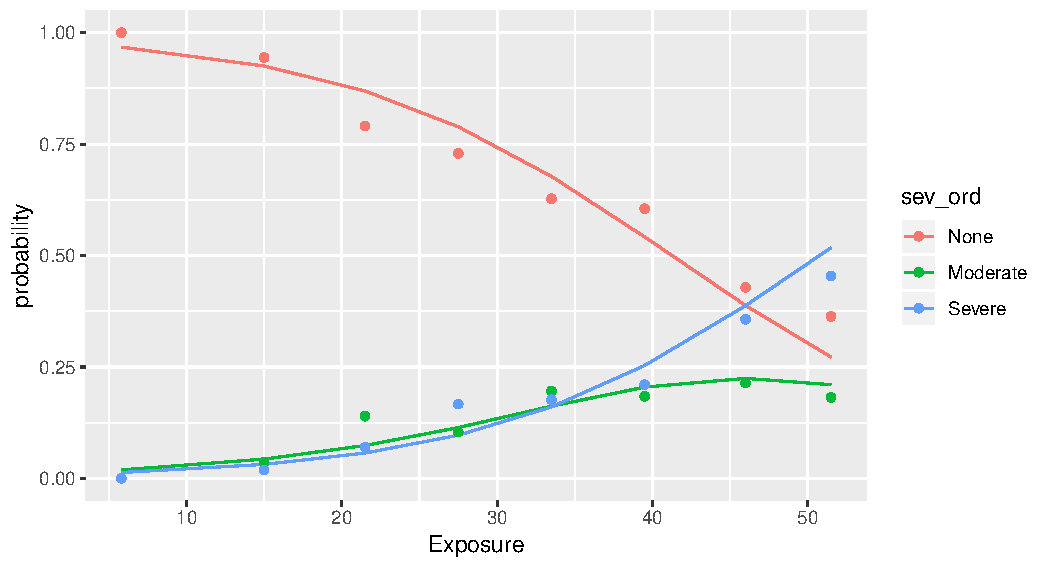
\includegraphics{figure/unnamed-chunk-101-1.pdf}
\caption{plot of chunk unnamed-chunk-101}
\end{figure}

\end{frame}

\begin{frame}[fragile]{Unordered responses}
\protect\hypertarget{unordered-responses}{}

\begin{itemize}
\item
  With unordered (nominal) responses, can use \emph{generalized logit}.
\item
  Example: 735 people, record age and sex (male 0, female 1), which of 3
  brands of some product preferred.
\item
  Data in \texttt{mlogit.csv} separated by commas (so \texttt{read\_csv}
  will work):
\end{itemize}

\begin{Shaded}
\begin{Highlighting}[]
\NormalTok{my_url <-}\StringTok{ "http://www.utsc.utoronto.ca/~butler/d29/mlogit.csv"}
\NormalTok{brandpref <-}\StringTok{ }\KeywordTok{read_csv}\NormalTok{(my_url)}
\end{Highlighting}
\end{Shaded}

\begin{verbatim}
## Parsed with column specification:
## cols(
##   brand = col_double(),
##   sex = col_double(),
##   age = col_double()
## )
\end{verbatim}

\end{frame}

\begin{frame}[fragile]{The data}
\protect\hypertarget{the-data-4}{}

\begin{Shaded}
\begin{Highlighting}[]
\NormalTok{brandpref}
\end{Highlighting}
\end{Shaded}

\begin{verbatim}
## # A tibble: 735 x 3
##    brand   sex   age
##    <dbl> <dbl> <dbl>
##  1     1     0    24
##  2     1     0    26
##  3     1     0    26
##  4     1     1    27
##  5     1     1    27
##  6     3     1    27
##  7     1     0    27
##  8     1     0    27
##  9     1     1    27
## 10     1     0    27
## # … with 725 more rows
\end{verbatim}

\end{frame}

\begin{frame}[fragile]{Bashing into shape, and fitting model}
\protect\hypertarget{bashing-into-shape-and-fitting-model}{}

\begin{itemize}
\tightlist
\item
  \texttt{sex} and \texttt{brand} not meaningful as numbers, so turn
  into factors:
\end{itemize}

\begin{Shaded}
\begin{Highlighting}[]
\NormalTok{brandpref <-}\StringTok{ }\NormalTok{brandpref }\OperatorTok
\StringTok{  }\KeywordTok{mutate}\NormalTok{(}\DataTypeTok{sex =} \KeywordTok{factor}\NormalTok{(sex)) }\OperatorTok
\StringTok{  }\KeywordTok{mutate}\NormalTok{(}\DataTypeTok{brand =} \KeywordTok{factor}\NormalTok{(brand))}
\end{Highlighting}
\end{Shaded}

\begin{itemize}
\tightlist
\item
  We use \texttt{multinom} from package \texttt{nnet}. Works like
  \texttt{polr}.
\end{itemize}

\begin{Shaded}
\begin{Highlighting}[]
\NormalTok{brands}\FloatTok{.1}\NormalTok{ <-}\StringTok{ }\KeywordTok{multinom}\NormalTok{(brand }\OperatorTok{~}\StringTok{ }\NormalTok{age }\OperatorTok{+}\StringTok{ }\NormalTok{sex, }\DataTypeTok{data =}\NormalTok{ brandpref)}
\end{Highlighting}
\end{Shaded}

\begin{verbatim}
## # weights:  12 (6 variable)
## initial  value 807.480032 
## iter  10 value 702.976983
## final  value 702.970704 
## converged
\end{verbatim}

\end{frame}

\begin{frame}[fragile]{Can we drop anything?}
\protect\hypertarget{can-we-drop-anything}{}

\begin{itemize}
\tightlist
\item
  Unfortunately \texttt{drop1} seems not to work:
\end{itemize}

\begin{Shaded}
\begin{Highlighting}[]
\KeywordTok{drop1}\NormalTok{(brands}\FloatTok{.1}\NormalTok{, }\DataTypeTok{test =} \StringTok{"Chisq"}\NormalTok{, }\DataTypeTok{trace =} \DecValTok{0}\NormalTok{)}
\end{Highlighting}
\end{Shaded}

\begin{verbatim}
## trying - age
\end{verbatim}

\begin{verbatim}
## Error in if (trace) {: argument is not interpretable as logical
\end{verbatim}

\begin{itemize}
\tightlist
\item
  so fall back on fitting model without what you want to test, and
  comparing using \texttt{anova}.
\end{itemize}

\end{frame}

\begin{frame}[fragile]{Do age/sex help predict brand? 1/2}
\protect\hypertarget{do-agesex-help-predict-brand-12}{}

Fit models without each of age and sex:

\begin{Shaded}
\begin{Highlighting}[]
\NormalTok{brands}\FloatTok{.2}\NormalTok{ <-}\StringTok{ }\KeywordTok{multinom}\NormalTok{(brand }\OperatorTok{~}\StringTok{ }\NormalTok{age, }\DataTypeTok{data =}\NormalTok{ brandpref)}
\end{Highlighting}
\end{Shaded}

\begin{verbatim}
## # weights:  9 (4 variable)
## initial  value 807.480032 
## iter  10 value 706.796323
## iter  10 value 706.796322
## final  value 706.796322 
## converged
\end{verbatim}

\begin{Shaded}
\begin{Highlighting}[]
\NormalTok{brands}\FloatTok{.3}\NormalTok{ <-}\StringTok{ }\KeywordTok{multinom}\NormalTok{(brand }\OperatorTok{~}\StringTok{ }\NormalTok{sex, }\DataTypeTok{data =}\NormalTok{ brandpref)}
\end{Highlighting}
\end{Shaded}

\begin{verbatim}
## # weights:  9 (4 variable)
## initial  value 807.480032 
## final  value 791.861266 
## converged
\end{verbatim}

\end{frame}

\begin{frame}[fragile]{Do age/sex help predict brand? 2/2}
\protect\hypertarget{do-agesex-help-predict-brand-22}{}

\scriptsize

\begin{Shaded}
\begin{Highlighting}[]
\KeywordTok{anova}\NormalTok{(brands}\FloatTok{.2}\NormalTok{, brands}\FloatTok{.1}\NormalTok{)}
\end{Highlighting}
\end{Shaded}

\begin{verbatim}
## Likelihood ratio tests of Multinomial Models
## 
## Response: brand
##       Model Resid. df Resid. Dev   Test    Df LR stat.    Pr(Chi)
## 1       age      1466   1413.593                                 
## 2 age + sex      1464   1405.941 1 vs 2     2 7.651236 0.02180495
\end{verbatim}

\begin{Shaded}
\begin{Highlighting}[]
\KeywordTok{anova}\NormalTok{(brands}\FloatTok{.3}\NormalTok{, brands}\FloatTok{.1}\NormalTok{)}
\end{Highlighting}
\end{Shaded}

\begin{verbatim}
## Likelihood ratio tests of Multinomial Models
## 
## Response: brand
##       Model Resid. df Resid. Dev   Test    Df LR stat. Pr(Chi)
## 1       sex      1466   1583.723                              
## 2 age + sex      1464   1405.941 1 vs 2     2 177.7811       0
\end{verbatim}

\normalsize

\end{frame}

\begin{frame}[fragile]{Do age/sex help predict brand? 3/3}
\protect\hypertarget{do-agesex-help-predict-brand-33}{}

\begin{itemize}
\item
  \texttt{age} definitely significant (second \texttt{anova})
\item
  \texttt{sex} seems significant also (first \texttt{anova})
\item
  Keep both.
\end{itemize}

\end{frame}

\begin{frame}[fragile]{Another way to build model}
\protect\hypertarget{another-way-to-build-model}{}

\begin{itemize}
\tightlist
\item
  Start from model with everything and run \texttt{step}:
\end{itemize}

\footnotesize

\begin{Shaded}
\begin{Highlighting}[]
\KeywordTok{step}\NormalTok{(brands}\FloatTok{.1}\NormalTok{, }\DataTypeTok{trace =} \DecValTok{0}\NormalTok{)}
\end{Highlighting}
\end{Shaded}

\begin{verbatim}
## trying - age 
## trying - sex
\end{verbatim}

\begin{verbatim}
## Call:
## multinom(formula = brand ~ age + sex, data = brandpref)
## 
## Coefficients:
##   (Intercept)       age      sex1
## 2   -11.77469 0.3682075 0.5238197
## 3   -22.72141 0.6859087 0.4659488
## 
## Residual Deviance: 1405.941 
## AIC: 1417.941
\end{verbatim}

\normalsize

\begin{itemize}
\tightlist
\item
  Final model contains both \texttt{age} and \texttt{sex} so neither
  could be removed.
\end{itemize}

\end{frame}

\begin{frame}[fragile]{Predictions: all possible combinations}
\protect\hypertarget{predictions-all-possible-combinations}{}

Create data frame with various age and sex:

\footnotesize

\begin{Shaded}
\begin{Highlighting}[]
\NormalTok{ages <-}\StringTok{ }\KeywordTok{c}\NormalTok{(}\DecValTok{24}\NormalTok{, }\DecValTok{28}\NormalTok{, }\DecValTok{32}\NormalTok{, }\DecValTok{35}\NormalTok{, }\DecValTok{38}\NormalTok{)}
\NormalTok{sexes <-}\StringTok{ }\KeywordTok{factor}\NormalTok{(}\DecValTok{0}\OperatorTok{:}\DecValTok{1}\NormalTok{)}
\NormalTok{new <-}\StringTok{ }\KeywordTok{crossing}\NormalTok{(}\DataTypeTok{age =}\NormalTok{ ages, }\DataTypeTok{sex =}\NormalTok{ sexes)}
\NormalTok{new}
\end{Highlighting}
\end{Shaded}

\begin{verbatim}
## # A tibble: 10 x 2
##      age sex  
##    <dbl> <fct>
##  1    24 0    
##  2    24 1    
##  3    28 0    
##  4    28 1    
##  5    32 0    
##  6    32 1    
##  7    35 0    
##  8    35 1    
##  9    38 0    
## 10    38 1
\end{verbatim}

\normalsize

\end{frame}

\begin{frame}[fragile]{Making predictions}
\protect\hypertarget{making-predictions}{}

\begin{Shaded}
\begin{Highlighting}[]
\NormalTok{p <-}\StringTok{ }\KeywordTok{predict}\NormalTok{(brands}\FloatTok{.1}\NormalTok{, new, }\DataTypeTok{type =} \StringTok{"probs"}\NormalTok{)}
\NormalTok{probs <-}\StringTok{ }\KeywordTok{cbind}\NormalTok{(new, p)}
\end{Highlighting}
\end{Shaded}

or

\begin{Shaded}
\begin{Highlighting}[]
\NormalTok{p }\OperatorTok\StringTok{ }\KeywordTok{as_tibble}\NormalTok{() }\OperatorTok\StringTok{ }
\StringTok{  }\KeywordTok{bind_cols}\NormalTok{(new) ->}\StringTok{ }\NormalTok{probs}
\end{Highlighting}
\end{Shaded}

\end{frame}

\begin{frame}[fragile]{The predictions}
\protect\hypertarget{the-predictions}{}

\small

\begin{Shaded}
\begin{Highlighting}[]
\NormalTok{probs}
\end{Highlighting}
\end{Shaded}

\begin{verbatim}
## # A tibble: 10 x 5
##       `1`    `2`     `3`   age sex  
##     <dbl>  <dbl>   <dbl> <dbl> <fct>
##  1 0.948  0.0502 0.00181    24 0    
##  2 0.915  0.0819 0.00279    24 1    
##  3 0.793  0.183  0.0236     28 0    
##  4 0.696  0.271  0.0329     28 1    
##  5 0.405  0.408  0.187      32 0    
##  6 0.291  0.495  0.214      32 1    
##  7 0.131  0.397  0.472      35 0    
##  8 0.0840 0.432  0.484      35 1    
##  9 0.0260 0.239  0.735      38 0    
## 10 0.0162 0.252  0.732      38 1
\end{verbatim}

\normalsize

\begin{itemize}
\item
  Young males (\texttt{sex=0}) prefer brand 1, but older males prefer
  brand 3.
\item
  Females similar, but like brand 1 less and brand 2 more.
\end{itemize}

\end{frame}

\begin{frame}[fragile]{Making a plot}
\protect\hypertarget{making-a-plot}{}

\begin{itemize}
\item
  Plot fitted probability against age, distinguishing brand by colour
  and gender by plotting symbol.
\item
  Also join points by lines, and distinguish lines by gender.
\item
  I thought about facetting, but this seems to come out clearer.
\item
  First need tidy data frame, by familiar process:
\end{itemize}

\begin{Shaded}
\begin{Highlighting}[]
\NormalTok{probs }\OperatorTok
\StringTok{  }\KeywordTok{gather}\NormalTok{(brand, probability, }\OperatorTok{-}\NormalTok{(age}\OperatorTok{:}\NormalTok{sex)) ->}\StringTok{ }\NormalTok{probs.long}
\end{Highlighting}
\end{Shaded}

\end{frame}

\begin{frame}[fragile]{The tidy data (random sample of rows)}
\protect\hypertarget{the-tidy-data-random-sample-of-rows}{}

\small

\begin{Shaded}
\begin{Highlighting}[]
\NormalTok{probs.long }\OperatorTok\StringTok{ }\KeywordTok{sample_n}\NormalTok{(}\DecValTok{10}\NormalTok{)}
\end{Highlighting}
\end{Shaded}

\begin{verbatim}
## # A tibble: 10 x 4
##      age sex   brand probability
##    <dbl> <fct> <chr>       <dbl>
##  1    38 1     1         0.0162 
##  2    35 1     3         0.484  
##  3    24 0     2         0.0502 
##  4    24 1     3         0.00279
##  5    32 1     3         0.214  
##  6    35 1     2         0.432  
##  7    28 1     2         0.271  
##  8    38 0     2         0.239  
##  9    38 0     1         0.0260 
## 10    38 1     2         0.252
\end{verbatim}

\normalsize

\end{frame}

\begin{frame}[fragile]{The plot}
\protect\hypertarget{the-plot-1}{}

\begin{Shaded}
\begin{Highlighting}[]
\KeywordTok{ggplot}\NormalTok{(probs.long, }\KeywordTok{aes}\NormalTok{(}
  \DataTypeTok{x =}\NormalTok{ age, }\DataTypeTok{y =}\NormalTok{ probability,}
  \DataTypeTok{colour =}\NormalTok{ brand, }\DataTypeTok{shape =}\NormalTok{ sex}
\NormalTok{)) }\OperatorTok{+}
\StringTok{  }\KeywordTok{geom_point}\NormalTok{() }\OperatorTok{+}\StringTok{ }\KeywordTok{geom_line}\NormalTok{(}\KeywordTok{aes}\NormalTok{(}\DataTypeTok{linetype =}\NormalTok{ sex))}
\end{Highlighting}
\end{Shaded}

\begin{figure}
\centering
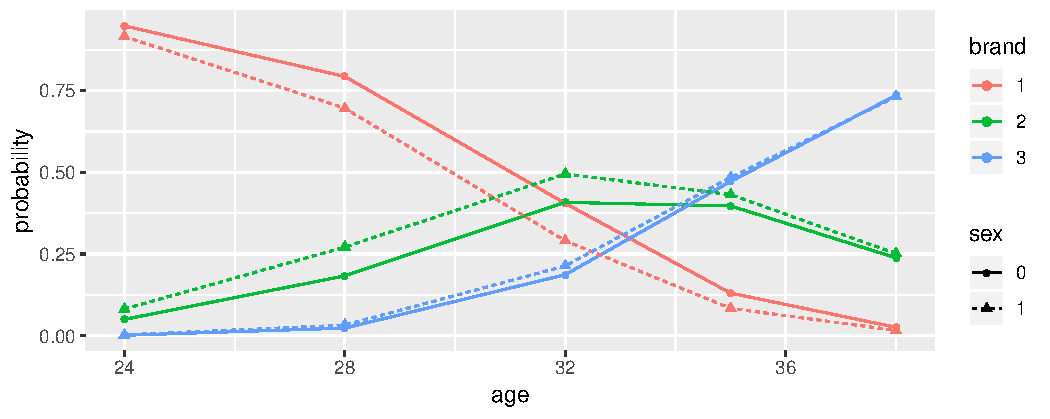
\includegraphics{figure/unnamed-chunk-116-1.pdf}
\caption{plot of chunk unnamed-chunk-116}
\end{figure}

\end{frame}

\begin{frame}{Digesting the plot}
\protect\hypertarget{digesting-the-plot}{}

\begin{itemize}
\item
  Brand vs.~age: younger people (of both genders) prefer brand 1, but
  older people (of both genders) prefer brand 3. (Explains significant
  age effect.)
\item
  Brand vs.~sex: females (dashed) like brand 1 less than males (solid),
  like brand 2 more (for all ages).
\item
  Not much brand difference between genders (solid and dashed lines of
  same colours close), but enough to be significant.
\item
  Model didn't include interaction, so modelled effect of gender on
  brand same for each age, modelled effect of age same for each gender.
\end{itemize}

\end{frame}

\begin{frame}[fragile]{Alternative data format}
\protect\hypertarget{alternative-data-format}{}

Summarize all people of same brand preference, same sex, same age on one
line of data file with frequency on end:

\begin{verbatim}
1 0 24 1
1 0 26 2
1 0 27 4
1 0 28 4
1 0 29 7
1 0 30 3
...
\end{verbatim}

Whole data set in 65 lines not 735! But how?

\end{frame}

\begin{frame}[fragile]{Getting alternative data format}
\protect\hypertarget{getting-alternative-data-format}{}

\begin{Shaded}
\begin{Highlighting}[]
\NormalTok{brandpref }\OperatorTok
\StringTok{  }\KeywordTok{group_by}\NormalTok{(age, sex, brand) }\OperatorTok
\StringTok{  }\KeywordTok{summarize}\NormalTok{(}\DataTypeTok{Freq =} \KeywordTok{n}\NormalTok{()) }\OperatorTok
\StringTok{  }\KeywordTok{ungroup}\NormalTok{() ->}\StringTok{ }\NormalTok{b}
\end{Highlighting}
\end{Shaded}

\begin{verbatim}
## [conflicted] `summarize` found in 2 packages.
## Either pick the one you want with `::` 
## * plyr::summarize
## * dplyr::summarize
## Or declare a preference with `conflict_prefer()`
## * conflict_prefer("summarize", "plyr")
## * conflict_prefer("summarize", "dplyr")
\end{verbatim}

\begin{Shaded}
\begin{Highlighting}[]
\NormalTok{b }\OperatorTok\StringTok{ }\KeywordTok{slice}\NormalTok{(}\DecValTok{1}\OperatorTok{:}\DecValTok{6}\NormalTok{)}
\end{Highlighting}
\end{Shaded}

\begin{verbatim}
## Error in eval(lhs, parent, parent): object 'b' not found
\end{verbatim}

\end{frame}

\begin{frame}[fragile]{Fitting models, almost the same}
\protect\hypertarget{fitting-models-almost-the-same}{}

\begin{itemize}
\item
  Just have to remember \texttt{weights} to incorporate frequencies.
\item
  Otherwise \texttt{multinom} assumes you have just 1 obs on each line!
\item
  Again turn (numerical) \texttt{sex} and \texttt{brand} into factors:
\end{itemize}

\footnotesize

\begin{Shaded}
\begin{Highlighting}[]
\NormalTok{b }\OperatorTok
\StringTok{  }\KeywordTok{mutate}\NormalTok{(}\DataTypeTok{sex =} \KeywordTok{factor}\NormalTok{(sex)) }\OperatorTok
\StringTok{  }\KeywordTok{mutate}\NormalTok{(}\DataTypeTok{brand =} \KeywordTok{factor}\NormalTok{(brand)) ->}\StringTok{ }\NormalTok{bf}
\end{Highlighting}
\end{Shaded}

\begin{verbatim}
## Error in eval(lhs, parent, parent): object 'b' not found
\end{verbatim}

\begin{Shaded}
\begin{Highlighting}[]
\NormalTok{b}\FloatTok{.1}\NormalTok{ <-}\StringTok{ }\KeywordTok{multinom}\NormalTok{(brand }\OperatorTok{~}\StringTok{ }\NormalTok{age }\OperatorTok{+}\StringTok{ }\NormalTok{sex, }\DataTypeTok{data =}\NormalTok{ bf, }\DataTypeTok{weights =}\NormalTok{ Freq)}
\end{Highlighting}
\end{Shaded}

\begin{verbatim}
## Error in is.data.frame(data): object 'bf' not found
\end{verbatim}

\begin{Shaded}
\begin{Highlighting}[]
\NormalTok{b}\FloatTok{.2}\NormalTok{ <-}\StringTok{ }\KeywordTok{multinom}\NormalTok{(brand }\OperatorTok{~}\StringTok{ }\NormalTok{age, }\DataTypeTok{data =}\NormalTok{ bf, }\DataTypeTok{weights =}\NormalTok{ Freq)}
\end{Highlighting}
\end{Shaded}

\begin{verbatim}
## Error in is.data.frame(data): object 'bf' not found
\end{verbatim}

\normalsize

\end{frame}

\begin{frame}[fragile]{P-value for \texttt{sex} identical}
\protect\hypertarget{p-value-for-sex-identical}{}

\footnotesize

\begin{Shaded}
\begin{Highlighting}[]
\KeywordTok{anova}\NormalTok{(b}\FloatTok{.2}\NormalTok{, b}\FloatTok{.1}\NormalTok{)}
\end{Highlighting}
\end{Shaded}

\begin{verbatim}
## Error in anova(b.2, b.1): object 'b.2' not found
\end{verbatim}

\normalsize

Same P-value as before, so we haven't changed anything important.

\end{frame}

\begin{frame}[fragile]{Including data on plot}
\protect\hypertarget{including-data-on-plot}{}

\begin{itemize}
\tightlist
\item
  Everyone's age given as whole number, so maybe not too many different
  ages with sensible amount of data at each:
\end{itemize}

\scriptsize

\begin{Shaded}
\begin{Highlighting}[]
\NormalTok{b }\OperatorTok
\StringTok{  }\KeywordTok{group_by}\NormalTok{(age) }\OperatorTok
\StringTok{  }\KeywordTok{summarize}\NormalTok{(}\DataTypeTok{total =} \KeywordTok{sum}\NormalTok{(Freq))}
\end{Highlighting}
\end{Shaded}

\begin{verbatim}
## Error in eval(lhs, parent, parent): object 'b' not found
\end{verbatim}

\normalsize

\end{frame}

\begin{frame}[fragile]{Comments and next}
\protect\hypertarget{comments-and-next}{}

\begin{itemize}
\item
  Not great (especially at low end), but live with it.
\item
  Need proportions of frequencies in each brand for each age-gender
  combination. Mimic what we did for miners:
\end{itemize}

\begin{Shaded}
\begin{Highlighting}[]
\NormalTok{b }\OperatorTok
\StringTok{  }\KeywordTok{group_by}\NormalTok{(age, sex) }\OperatorTok
\StringTok{  }\KeywordTok{mutate}\NormalTok{(}\DataTypeTok{proportion =}\NormalTok{ Freq }\OperatorTok{/}\StringTok{ }\KeywordTok{sum}\NormalTok{(Freq)) ->}\StringTok{ }\NormalTok{brands}
\end{Highlighting}
\end{Shaded}

\begin{verbatim}
## Error in eval(lhs, parent, parent): object 'b' not found
\end{verbatim}

\end{frame}

\begin{frame}[fragile]{Checking proportions for age 32}
\protect\hypertarget{checking-proportions-for-age-32}{}

\small

\begin{Shaded}
\begin{Highlighting}[]
\NormalTok{brands }\OperatorTok\StringTok{ }\KeywordTok{filter}\NormalTok{(age }\OperatorTok{==}\StringTok{ }\DecValTok{32}\NormalTok{)}
\end{Highlighting}
\end{Shaded}

\begin{verbatim}
## Error in eval(lhs, parent, parent): object 'brands' not found
\end{verbatim}

\normalsize

\begin{itemize}
\item
  First three proportions (males) add up to 1.
\item
  Last three proportions (females) add up to 1.
\item
  So looks like proportions of right thing.
\end{itemize}

\end{frame}

\begin{frame}[fragile]{Attempting plot}
\protect\hypertarget{attempting-plot}{}

\begin{itemize}
\item
  Take code from previous plot and:
\item
  remove \texttt{geom\_point} for fitted values
\item
  add \texttt{geom\_point} with correct \texttt{data=} and \texttt{aes}
  to plot data.
\end{itemize}

\begin{Shaded}
\begin{Highlighting}[]
\NormalTok{g <-}\StringTok{ }\KeywordTok{ggplot}\NormalTok{(probs.long, }\KeywordTok{aes}\NormalTok{(}
  \DataTypeTok{x =}\NormalTok{ age, }\DataTypeTok{y =}\NormalTok{ probability,}
  \DataTypeTok{colour =}\NormalTok{ brand, }\DataTypeTok{shape =}\NormalTok{ sex}
\NormalTok{)) }\OperatorTok{+}
\StringTok{  }\KeywordTok{geom_line}\NormalTok{(}\KeywordTok{aes}\NormalTok{(}\DataTypeTok{linetype =}\NormalTok{ sex)) }\OperatorTok{+}
\StringTok{  }\KeywordTok{geom_point}\NormalTok{(}\DataTypeTok{data =}\NormalTok{ brands, }\KeywordTok{aes}\NormalTok{(}\DataTypeTok{y =}\NormalTok{ proportion))}
\end{Highlighting}
\end{Shaded}

\begin{verbatim}
## Error in fortify(data): object 'brands' not found
\end{verbatim}

\begin{itemize}
\tightlist
\item
  Data seem to correspond more or less to fitted curves:
\end{itemize}

\end{frame}

\begin{frame}[fragile]{The plot}
\protect\hypertarget{the-plot-2}{}

\begin{Shaded}
\begin{Highlighting}[]
\NormalTok{g}
\end{Highlighting}
\end{Shaded}

\begin{figure}
\centering
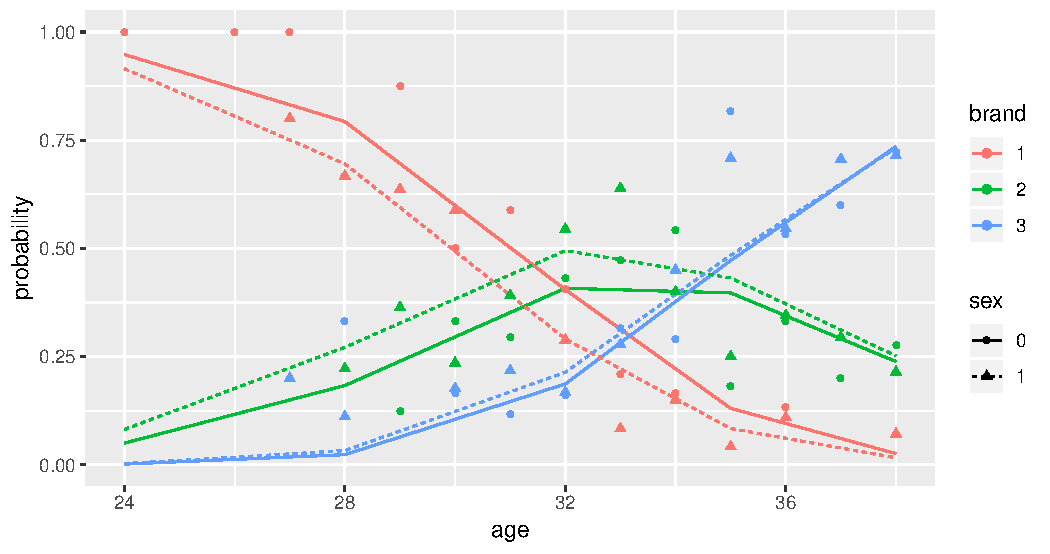
\includegraphics{figure/unnamed-chunk-123-1.pdf}
\caption{plot of chunk unnamed-chunk-123}
\end{figure}

\end{frame}

\begin{frame}[fragile]{But\ldots}
\protect\hypertarget{but-1}{}

\begin{itemize}
\item
  Some of the plotted points based on a lot of people, and some only a
  few.
\item
  Idea: make the \emph{size} of plotted point bigger if point based on a
  lot of people (in \texttt{Freq}).
\item
  Hope that larger points then closer to predictions.
\item
  Code:
\end{itemize}

\footnotesize

\begin{Shaded}
\begin{Highlighting}[]
\NormalTok{g <-}\StringTok{ }\KeywordTok{ggplot}\NormalTok{(probs.long, }\KeywordTok{aes}\NormalTok{(}
  \DataTypeTok{x =}\NormalTok{ age, }\DataTypeTok{y =}\NormalTok{ probability,}
  \DataTypeTok{colour =}\NormalTok{ brand, }\DataTypeTok{shape =}\NormalTok{ sex}
\NormalTok{)) }\OperatorTok{+}
\StringTok{  }\KeywordTok{geom_line}\NormalTok{(}\KeywordTok{aes}\NormalTok{(}\DataTypeTok{linetype =}\NormalTok{ sex)) }\OperatorTok{+}
\StringTok{  }\KeywordTok{geom_point}\NormalTok{(}
    \DataTypeTok{data =}\NormalTok{ brands,}
    \KeywordTok{aes}\NormalTok{(}\DataTypeTok{y =}\NormalTok{ proportion, }\DataTypeTok{size =}\NormalTok{ Freq)}
\NormalTok{  )}
\end{Highlighting}
\end{Shaded}

\begin{verbatim}
## Error in fortify(data): object 'brands' not found
\end{verbatim}

\normalsize

\end{frame}

\begin{frame}[fragile]{The plot}
\protect\hypertarget{the-plot-3}{}

\begin{Shaded}
\begin{Highlighting}[]
\NormalTok{g}
\end{Highlighting}
\end{Shaded}

\begin{figure}
\centering
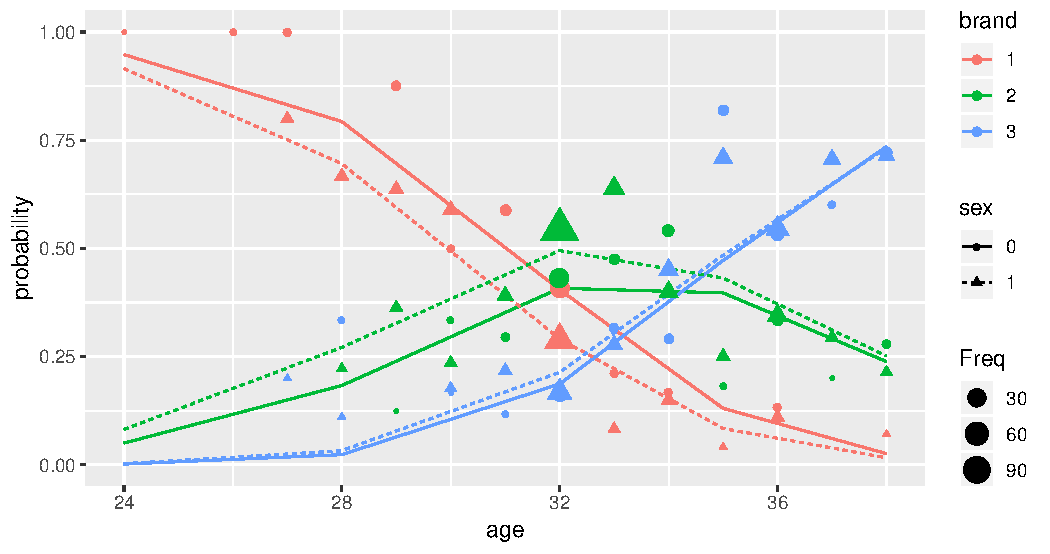
\includegraphics{figure/unnamed-chunk-125-1.pdf}
\caption{plot of chunk unnamed-chunk-125}
\end{figure}

\end{frame}

\begin{frame}[fragile]{Trying interaction between age and gender}
\protect\hypertarget{trying-interaction-between-age-and-gender}{}

\scriptsize

\begin{Shaded}
\begin{Highlighting}[]
\NormalTok{b}\FloatTok{.4}\NormalTok{ <-}\StringTok{ }\KeywordTok{update}\NormalTok{(b}\FloatTok{.1}\NormalTok{, . }\OperatorTok{~}\StringTok{ }\NormalTok{. }\OperatorTok{+}\StringTok{ }\NormalTok{age}\OperatorTok{:}\NormalTok{sex)}
\end{Highlighting}
\end{Shaded}

\begin{verbatim}
## Error in update(b.1, . ~ . + age:sex): object 'b.1' not found
\end{verbatim}

\begin{Shaded}
\begin{Highlighting}[]
\KeywordTok{anova}\NormalTok{(b}\FloatTok{.1}\NormalTok{, b}\FloatTok{.4}\NormalTok{)}
\end{Highlighting}
\end{Shaded}

\begin{verbatim}
## Error in anova(b.1, b.4): object 'b.1' not found
\end{verbatim}

\normalsize

\begin{itemize}
\tightlist
\item
  No evidence that effect of age on brand preference differs for the two
  genders.
\end{itemize}

\end{frame}

\hypertarget{survival-analysis}{%
\section{Survival analysis}\label{survival-analysis}}

\begin{frame}{Survival analysis}
\protect\hypertarget{survival-analysis-1}{}

\begin{itemize}
\item
  So far, have seen:

  \begin{itemize}
  \item
    response variable counted or measured (regression)
  \item
    response variable categorized (logistic regression)
  \end{itemize}
\end{itemize}

and have predicted response from explanatory variables.

\begin{itemize}
\item
  But what if response is time until event (eg. time of survival after
  surgery)?
\item
  Additional complication: event might not have happened at end of study
  (eg. patient still alive). But knowing that patient has ``not died
  yet'' presumably informative. Such data called \emph{censored}.
\item
  Enter \emph{survival analysis}, in particular the ``Cox proportional
  hazards model''.
\item
  Explanatory variables in this context often called \emph{covariates}.
\end{itemize}

\end{frame}

\begin{frame}{Example: still dancing?}
\protect\hypertarget{example-still-dancing}{}

\begin{itemize}
\item
  12 women who have just started taking dancing lessons are followed for
  up to a year, to see whether they are still taking dancing lessons, or
  have quit. The ``event'' here is ``quit''.
\item
  This might depend on:

  \begin{itemize}
  \item
    a treatment (visit to a dance competition)
  \item
    woman's age (at start of study).
  \end{itemize}
\end{itemize}

\end{frame}

\begin{frame}[fragile]{Data}
\protect\hypertarget{data}{}

\normalsize

\begin{verbatim}
Months  Quit   Treatment Age
1        1        0      16
2        1        0      24
2        1        0      18
3        0        0      27
4        1        0      25
7        1        1      26
8        1        1      36
10       1        1      38
10       0        1      45
12       1        1      47
\end{verbatim}

\normalsize

\end{frame}

\begin{frame}[fragile]{About the data}
\protect\hypertarget{about-the-data}{}

\begin{itemize}
\item
  \texttt{months} and \texttt{quit} are kind of combined response:

  \begin{itemize}
  \item
    \texttt{Months} is number of months a woman was actually observed
    dancing
  \item
    \texttt{quit} is 1 if woman quit, 0 if still dancing at end of
    study.
  \end{itemize}
\item
  Treatment is 1 if woman went to dance competition, 0 otherwise.
\item
  Fit model and see whether \texttt{Age} or \texttt{Treatment} have
  effect on survival.
\item
  Want to do predictions for probabilities of still dancing as they
  depend on whatever is significant, and draw plot.
\end{itemize}

\end{frame}

\begin{frame}[fragile]{Packages (for this section)}
\protect\hypertarget{packages-for-this-section}{}

\begin{itemize}
\item
  Install packages \texttt{survival} and \texttt{survminer} if not done.
\item
  Load \texttt{survival}, \texttt{survminer}, \texttt{broom} and
  \texttt{tidyverse}:
\end{itemize}

\begin{Shaded}
\begin{Highlighting}[]
\KeywordTok{library}\NormalTok{(tidyverse)}
\KeywordTok{library}\NormalTok{(survival)}
\KeywordTok{library}\NormalTok{(survminer)}
\KeywordTok{library}\NormalTok{(broom)}
\end{Highlighting}
\end{Shaded}

\end{frame}

\begin{frame}[fragile]{Read data}
\protect\hypertarget{read-data}{}

\begin{itemize}
\tightlist
\item
  Column-aligned:
\end{itemize}

\normalsize

\begin{Shaded}
\begin{Highlighting}[]
\NormalTok{url <-}\StringTok{ "http://www.utsc.utoronto.ca/~butler/d29/dancing.txt"}
\NormalTok{dance <-}\StringTok{ }\KeywordTok{read_table}\NormalTok{(url)}
\end{Highlighting}
\end{Shaded}

\begin{verbatim}
## Parsed with column specification:
## cols(
##   Months = col_double(),
##   Quit = col_double(),
##   Treatment = col_double(),
##   Age = col_double()
## )
\end{verbatim}

\normalsize

\end{frame}

\begin{frame}[fragile]{The data}
\protect\hypertarget{the-data-5}{}

\small

\begin{Shaded}
\begin{Highlighting}[]
\NormalTok{dance}
\end{Highlighting}
\end{Shaded}

\begin{verbatim}
## # A tibble: 12 x 4
##    Months  Quit Treatment   Age
##     <dbl> <dbl>     <dbl> <dbl>
##  1      1     1         0    16
##  2      2     1         0    24
##  3      2     1         0    18
##  4      3     0         0    27
##  5      4     1         0    25
##  6      5     1         0    21
##  7     11     1         0    55
##  8      7     1         1    26
##  9      8     1         1    36
## 10     10     1         1    38
## 11     10     0         1    45
## 12     12     1         1    47
\end{verbatim}

\normalsize

\end{frame}

\begin{frame}[fragile]{Examine response and fit model}
\protect\hypertarget{examine-response-and-fit-model}{}

\begin{itemize}
\tightlist
\item
  Response variable (has to be outside data frame):
\end{itemize}

\small

\begin{Shaded}
\begin{Highlighting}[]
\NormalTok{mth <-}\StringTok{ }\KeywordTok{with}\NormalTok{(dance, }\KeywordTok{Surv}\NormalTok{(Months, Quit))}
\NormalTok{mth}
\end{Highlighting}
\end{Shaded}

\begin{verbatim}
##  [1]  1   2   2   3+  4   5  11   7   8  10  10+ 12
\end{verbatim}

\normalsize

\begin{itemize}
\tightlist
\item
  Then fit model, predicting \texttt{mth} from explanatories:
\end{itemize}

\begin{Shaded}
\begin{Highlighting}[]
\NormalTok{dance}\FloatTok{.1}\NormalTok{ <-}\StringTok{ }\KeywordTok{coxph}\NormalTok{(mth }\OperatorTok{~}\StringTok{ }\NormalTok{Treatment }\OperatorTok{+}\StringTok{ }\NormalTok{Age, }\DataTypeTok{data =}\NormalTok{ dance)}
\end{Highlighting}
\end{Shaded}

\end{frame}

\begin{frame}[fragile]{Output looks a lot like regression}
\protect\hypertarget{output-looks-a-lot-like-regression}{}

\scriptsize

\begin{Shaded}
\begin{Highlighting}[]
\KeywordTok{summary}\NormalTok{(dance}\FloatTok{.1}\NormalTok{)}
\end{Highlighting}
\end{Shaded}

\begin{verbatim}
## Call:
## coxph(formula = mth ~ Treatment + Age, data = dance)
## 
##   n= 12, number of events= 10 
## 
##               coef exp(coef) se(coef)      z Pr(>|z|)  
## Treatment -4.44915   0.01169  2.60929 -1.705   0.0882 .
## Age       -0.36619   0.69337  0.15381 -2.381   0.0173 *
## ---
## Signif. codes:  
## 0 '***' 0.001 '**' 0.01 '*' 0.05 '.' 0.1 ' ' 1
## 
##           exp(coef) exp(-coef) lower .95 upper .95
## Treatment   0.01169     85.554 7.026e-05    1.9444
## Age         0.69337      1.442 5.129e-01    0.9373
## 
## Concordance= 0.964  (se = 0.039 )
## Likelihood ratio test= 21.68  on 2 df,   p=2e-05
## Wald test            = 5.67  on 2 df,   p=0.06
## Score (logrank) test = 14.75  on 2 df,   p=6e-04
\end{verbatim}

\normalsize

\end{frame}

\begin{frame}[fragile]{Conclusions}
\protect\hypertarget{conclusions-1}{}

\begin{itemize}
\item
  Use \(\alpha=0.10\) here since not much data.
\item
  Three tests at bottom like global F-test. Consensus that something
  predicts survival time (whether or not dancer quit and how long it
  took).
\item
  \texttt{Age} (definitely), \texttt{Treatment} (marginally) both
  predict survival time.
\end{itemize}

\end{frame}

\begin{frame}[fragile]{Model checking}
\protect\hypertarget{model-checking}{}

\begin{itemize}
\item
  With regression, usually plot residuals against fitted values.
\item
  Not quite same here (nonlinear model), but ``martingale residuals''
  should have no pattern vs.~``linear predictor''.
\item
  \texttt{ggcoxdiagnostics} from package \texttt{survminer} makes plot,
  to which we add smooth. If smooth trend more or less straight across,
  model OK.
\item
  Martingale residuals can go very negative, so won't always look
  normal.
\end{itemize}

\end{frame}

\begin{frame}[fragile]{Martingale residual plot for dance data}
\protect\hypertarget{martingale-residual-plot-for-dance-data}{}

This looks good (with only 12 points):

\begin{Shaded}
\begin{Highlighting}[]
\KeywordTok{ggcoxdiagnostics}\NormalTok{(dance}\FloatTok{.1}\NormalTok{) }\OperatorTok{+}\StringTok{ }\KeywordTok{geom_smooth}\NormalTok{(}\DataTypeTok{se =}\NormalTok{ F)}
\end{Highlighting}
\end{Shaded}

\begin{verbatim}
## `geom_smooth()` using method = 'loess' and formula 'y ~ x'
\end{verbatim}

\begin{figure}
\centering
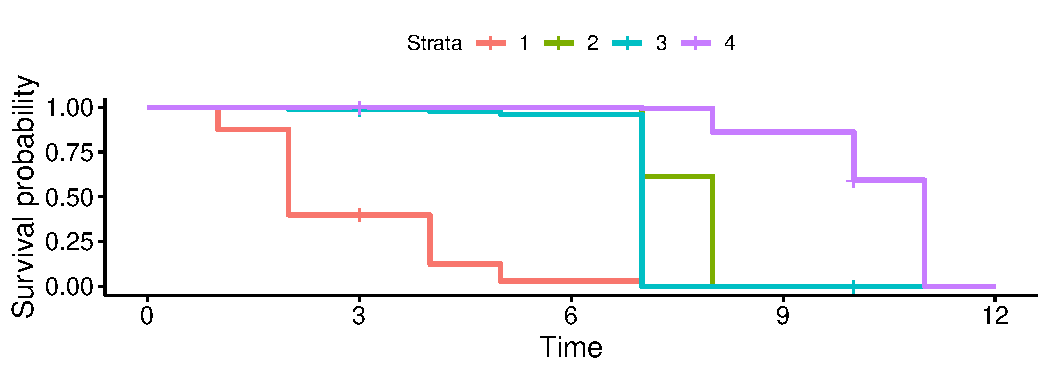
\includegraphics{figure/unnamed-chunk-134-1.pdf}
\caption{plot of chunk unnamed-chunk-134}
\end{figure}

\end{frame}

\begin{frame}[fragile]{Predicted survival probs}
\protect\hypertarget{predicted-survival-probs-1}{}

\begin{itemize}
\tightlist
\item
  The function we use is called \texttt{survfit}, though actually works
  rather like \texttt{predict}.
\item
  First create a data frame of values to predict from. We'll do all
  combos of ages 20 and 40, treatment and not, using \texttt{crossing}
  to get all the combos:
\end{itemize}

\small

\begin{Shaded}
\begin{Highlighting}[]
\NormalTok{treatments <-}\StringTok{ }\KeywordTok{c}\NormalTok{(}\DecValTok{0}\NormalTok{, }\DecValTok{1}\NormalTok{)}
\NormalTok{ages <-}\StringTok{ }\KeywordTok{c}\NormalTok{(}\DecValTok{20}\NormalTok{, }\DecValTok{40}\NormalTok{)}
\NormalTok{dance.new <-}\StringTok{ }\KeywordTok{crossing}\NormalTok{(}\DataTypeTok{Treatment =}\NormalTok{ treatments, }\DataTypeTok{Age =}\NormalTok{ ages)}
\NormalTok{dance.new}
\end{Highlighting}
\end{Shaded}

\begin{verbatim}
## # A tibble: 4 x 2
##   Treatment   Age
##       <dbl> <dbl>
## 1         0    20
## 2         0    40
## 3         1    20
## 4         1    40
\end{verbatim}

\normalsize

\end{frame}

\begin{frame}[fragile]{The predictions}
\protect\hypertarget{the-predictions-1}{}

One prediction \emph{for each time} for each combo of age and treatment
in \texttt{dance.new}:

\footnotesize

\begin{Shaded}
\begin{Highlighting}[]
\NormalTok{s <-}\StringTok{ }\KeywordTok{survfit}\NormalTok{(dance}\FloatTok{.1}\NormalTok{, }\DataTypeTok{newdata =}\NormalTok{ dance.new, }\DataTypeTok{data =}\NormalTok{ dance)}
\KeywordTok{summary}\NormalTok{(s)}
\end{Highlighting}
\end{Shaded}

\begin{verbatim}
## Call: survfit(formula = dance.1, newdata = dance.new, data = dance)
## 
##  time n.risk n.event survival1 survival2 survival3 survival4
##     1     12       1  8.76e-01  1.00e+00  9.98e-01     1.000
##     2     11       2  3.99e-01  9.99e-01  9.89e-01     1.000
##     4      8       1  1.24e-01  9.99e-01  9.76e-01     1.000
##     5      7       1  2.93e-02  9.98e-01  9.60e-01     1.000
##     7      6       1 2.96e-323  6.13e-01  1.70e-04     0.994
##     8      5       1  0.00e+00  2.99e-06  1.35e-98     0.862
##    10      4       1  0.00e+00  3.61e-20  0.00e+00     0.593
##    11      2       1  0.00e+00  0.00e+00  0.00e+00     0.000
##    12      1       1  0.00e+00  0.00e+00  0.00e+00     0.000
\end{verbatim}

\normalsize

\end{frame}

\begin{frame}[fragile]{Conclusions from predicted probs}
\protect\hypertarget{conclusions-from-predicted-probs}{}

\begin{itemize}
\item
  Older women more likely to be still dancing than younger women
  (compare ``profiles'' for same treatment group).
\item
  Effect of treatment seems to be to increase prob of still dancing
  (compare ``profiles'' for same age for treatment group vs.~not)
\item
  Would be nice to see this on a graph. This is \texttt{ggsurvplot} from
  package \texttt{survminer}:
\end{itemize}

\begin{Shaded}
\begin{Highlighting}[]
\NormalTok{g <-}\StringTok{ }\KeywordTok{ggsurvplot}\NormalTok{(s, }\DataTypeTok{conf.int =}\NormalTok{ F)}
\end{Highlighting}
\end{Shaded}

\begin{itemize}
\tightlist
\item
  uses ``strata'' thus (\texttt{dance.new}):
\end{itemize}

\footnotesize

\begin{verbatim}
## # A tibble: 4 x 2
##   Treatment   Age
##       <dbl> <dbl>
## 1         0    20
## 2         0    40
## 3         1    20
## 4         1    40
\end{verbatim}

\normalsize

\end{frame}

\begin{frame}[fragile]{Plotting survival probabilities}
\protect\hypertarget{plotting-survival-probabilities}{}

\begin{Shaded}
\begin{Highlighting}[]
\NormalTok{g}
\end{Highlighting}
\end{Shaded}

\begin{figure}
\centering
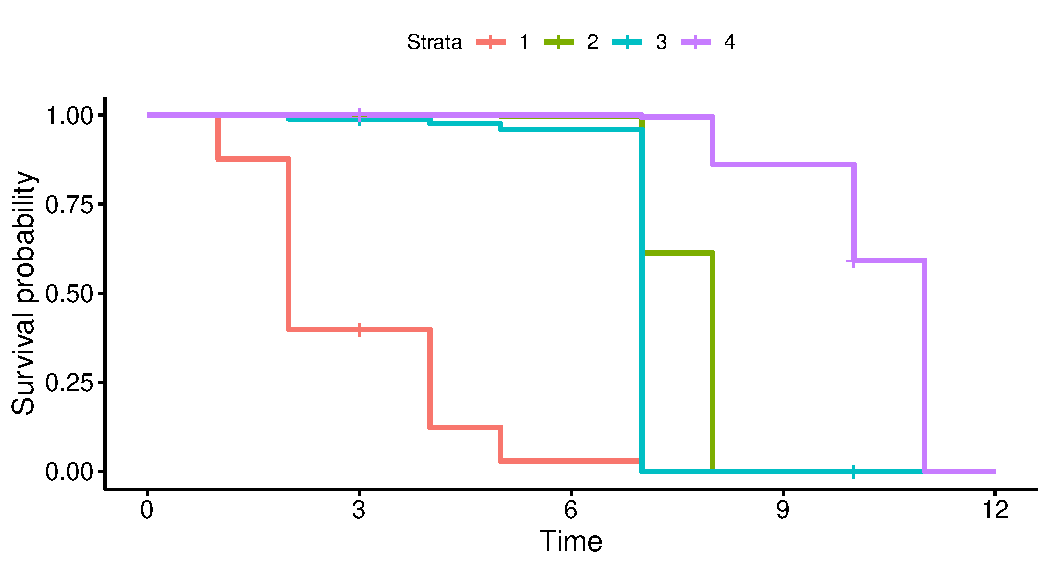
\includegraphics{figure/survival-plot-1.pdf}
\caption{plot of chunk survival-plot}
\end{figure}

\end{frame}

\begin{frame}{Discussion}
\protect\hypertarget{discussion}{}

\begin{itemize}
\item
  Survivor curve farther to the right is better (better chance of
  surviving longer).
\item
  Best is age 40 with treatment, worst age 20 without.
\item
  Appears to be:

  \begin{itemize}
  \item
    age effect (40 better than 20)
  \item
    treatment effect (treatment better than not)
  \item
    In analysis, treatment effect only marginally significant.
  \end{itemize}
\end{itemize}

\end{frame}

\begin{frame}[fragile]{A more realistic example: lung cancer}
\protect\hypertarget{a-more-realistic-example-lung-cancer}{}

\begin{itemize}
\item
  When you load in an R package, get data sets to illustrate functions
  in the package.
\item
  One such is \texttt{lung}. Data set measuring survival in patients
  with advanced lung cancer.
\item
  Along with survival time, number of ``performance scores'' included,
  measuring how well patients can perform daily activities.
\item
  Sometimes high good, but sometimes bad!
\item
  Variables below, from the data set help file (\texttt{?lung}).
\end{itemize}

\end{frame}

\begin{frame}{The variables}
\protect\hypertarget{the-variables}{}

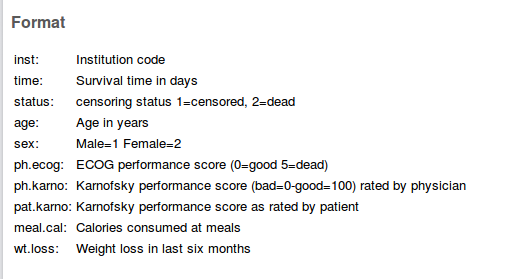
\includegraphics{lung-cancer-data.png}

\end{frame}

\begin{frame}[fragile]{Uh oh, missing values}
\protect\hypertarget{uh-oh-missing-values}{}

\scriptsize

\begin{Shaded}
\begin{Highlighting}[]
\NormalTok{lung }\OperatorTok\StringTok{ }\KeywordTok{slice}\NormalTok{(}\DecValTok{1}\OperatorTok{:}\DecValTok{16}\NormalTok{)}
\end{Highlighting}
\end{Shaded}

\begin{verbatim}
##    inst time status age sex ph.ecog ph.karno pat.karno meal.cal wt.loss
## 1     3  306      2  74   1       1       90       100     1175      NA
## 2     3  455      2  68   1       0       90        90     1225      15
## 3     3 1010      1  56   1       0       90        90       NA      15
## 4     5  210      2  57   1       1       90        60     1150      11
## 5     1  883      2  60   1       0      100        90       NA       0
## 6    12 1022      1  74   1       1       50        80      513       0
## 7     7  310      2  68   2       2       70        60      384      10
## 8    11  361      2  71   2       2       60        80      538       1
## 9     1  218      2  53   1       1       70        80      825      16
## 10    7  166      2  61   1       2       70        70      271      34
## 11    6  170      2  57   1       1       80        80     1025      27
## 12   16  654      2  68   2       2       70        70       NA      23
## 13   11  728      2  68   2       1       90        90       NA       5
## 14   21   71      2  60   1      NA       60        70     1225      32
## 15   12  567      2  57   1       1       80        70     2600      60
## 16    1  144      2  67   1       1       80        90       NA      15
\end{verbatim}

\normalsize

\end{frame}

\begin{frame}[fragile]{A closer look}
\protect\hypertarget{a-closer-look}{}

\tiny

\begin{Shaded}
\begin{Highlighting}[]
\KeywordTok{summary}\NormalTok{(lung)}
\end{Highlighting}
\end{Shaded}

\begin{verbatim}
##       inst            time            status           age             sex       
##  Min.   : 1.00   Min.   :   5.0   Min.   :1.000   Min.   :39.00   Min.   :1.000  
##  1st Qu.: 3.00   1st Qu.: 166.8   1st Qu.:1.000   1st Qu.:56.00   1st Qu.:1.000  
##  Median :11.00   Median : 255.5   Median :2.000   Median :63.00   Median :1.000  
##  Mean   :11.09   Mean   : 305.2   Mean   :1.724   Mean   :62.45   Mean   :1.395  
##  3rd Qu.:16.00   3rd Qu.: 396.5   3rd Qu.:2.000   3rd Qu.:69.00   3rd Qu.:2.000  
##  Max.   :33.00   Max.   :1022.0   Max.   :2.000   Max.   :82.00   Max.   :2.000  
##  NA's   :1                                                                       
##     ph.ecog          ph.karno        pat.karno         meal.cal         wt.loss       
##  Min.   :0.0000   Min.   : 50.00   Min.   : 30.00   Min.   :  96.0   Min.   :-24.000  
##  1st Qu.:0.0000   1st Qu.: 75.00   1st Qu.: 70.00   1st Qu.: 635.0   1st Qu.:  0.000  
##  Median :1.0000   Median : 80.00   Median : 80.00   Median : 975.0   Median :  7.000  
##  Mean   :0.9515   Mean   : 81.94   Mean   : 79.96   Mean   : 928.8   Mean   :  9.832  
##  3rd Qu.:1.0000   3rd Qu.: 90.00   3rd Qu.: 90.00   3rd Qu.:1150.0   3rd Qu.: 15.750  
##  Max.   :3.0000   Max.   :100.00   Max.   :100.00   Max.   :2600.0   Max.   : 68.000  
##  NA's   :1        NA's   :1        NA's   :3        NA's   :47       NA's   :14
\end{verbatim}

\normalsize

\end{frame}

\begin{frame}[fragile]{Remove obs with \emph{any} missing values}
\protect\hypertarget{remove-obs-with-any-missing-values}{}

\small

\begin{Shaded}
\begin{Highlighting}[]
\NormalTok{lung }\OperatorTok\StringTok{ }\KeywordTok{drop_na}\NormalTok{() ->}\StringTok{ }\NormalTok{lung.complete}
\NormalTok{lung.complete }\OperatorTok
\StringTok{  }\KeywordTok{select}\NormalTok{(meal.cal}\OperatorTok{:}\NormalTok{wt.loss) }\OperatorTok
\StringTok{  }\KeywordTok{slice}\NormalTok{(}\DecValTok{1}\OperatorTok{:}\DecValTok{10}\NormalTok{)}
\end{Highlighting}
\end{Shaded}

\begin{verbatim}
##    meal.cal wt.loss
## 1      1225      15
## 2      1150      11
## 3       513       0
## 4       384      10
## 5       538       1
## 6       825      16
## 7       271      34
## 8      1025      27
## 9      2600      60
## 10     1150      -5
\end{verbatim}

\normalsize

Missing values seem to be gone.

\end{frame}

\begin{frame}[fragile]{Check!}
\protect\hypertarget{check}{}

\tiny

\begin{Shaded}
\begin{Highlighting}[]
\KeywordTok{summary}\NormalTok{(lung.complete)}
\end{Highlighting}
\end{Shaded}

\begin{verbatim}
##       inst            time            status           age             sex       
##  Min.   : 1.00   Min.   :   5.0   Min.   :1.000   Min.   :39.00   Min.   :1.000  
##  1st Qu.: 3.00   1st Qu.: 174.5   1st Qu.:1.000   1st Qu.:57.00   1st Qu.:1.000  
##  Median :11.00   Median : 268.0   Median :2.000   Median :64.00   Median :1.000  
##  Mean   :10.71   Mean   : 309.9   Mean   :1.719   Mean   :62.57   Mean   :1.383  
##  3rd Qu.:15.00   3rd Qu.: 419.5   3rd Qu.:2.000   3rd Qu.:70.00   3rd Qu.:2.000  
##  Max.   :32.00   Max.   :1022.0   Max.   :2.000   Max.   :82.00   Max.   :2.000  
##     ph.ecog          ph.karno        pat.karno         meal.cal         wt.loss       
##  Min.   :0.0000   Min.   : 50.00   Min.   : 30.00   Min.   :  96.0   Min.   :-24.000  
##  1st Qu.:0.0000   1st Qu.: 70.00   1st Qu.: 70.00   1st Qu.: 619.0   1st Qu.:  0.000  
##  Median :1.0000   Median : 80.00   Median : 80.00   Median : 975.0   Median :  7.000  
##  Mean   :0.9581   Mean   : 82.04   Mean   : 79.58   Mean   : 929.1   Mean   :  9.719  
##  3rd Qu.:1.0000   3rd Qu.: 90.00   3rd Qu.: 90.00   3rd Qu.:1162.5   3rd Qu.: 15.000  
##  Max.   :3.0000   Max.   :100.00   Max.   :100.00   Max.   :2600.0   Max.   : 68.000
\end{verbatim}

\normalsize

No missing values left.

\end{frame}

\begin{frame}[fragile]{Model 1: use everything except \texttt{inst}}
\protect\hypertarget{model-1-use-everything-except-inst}{}

\footnotesize

\begin{Shaded}
\begin{Highlighting}[]
\KeywordTok{names}\NormalTok{(lung.complete)}
\end{Highlighting}
\end{Shaded}

\begin{verbatim}
##  [1] "inst"      "time"      "status"    "age"       "sex"       "ph.ecog"   "ph.karno" 
##  [8] "pat.karno" "meal.cal"  "wt.loss"
\end{verbatim}

\normalsize

\begin{itemize}
\tightlist
\item
  Event was death, goes with \texttt{status} of 2:
\end{itemize}

\begin{Shaded}
\begin{Highlighting}[]
\NormalTok{resp <-}\StringTok{ }\KeywordTok{with}\NormalTok{(lung.complete, }\KeywordTok{Surv}\NormalTok{(time, status }\OperatorTok{==}\StringTok{ }\DecValTok{2}\NormalTok{))}
\NormalTok{lung}\FloatTok{.1}\NormalTok{ <-}\StringTok{ }\KeywordTok{coxph}\NormalTok{(resp }\OperatorTok{~}\StringTok{ }\NormalTok{. }\OperatorTok{-}\StringTok{ }\NormalTok{inst }\OperatorTok{-}\StringTok{ }\NormalTok{time }\OperatorTok{-}\StringTok{ }\NormalTok{status,}
  \DataTypeTok{data =}\NormalTok{ lung.complete}
\NormalTok{)}
\end{Highlighting}
\end{Shaded}

``Dot'' means ``all the other variables''.

\end{frame}

\begin{frame}[fragile]{\texttt{summary} of model 1: too tiny to see!}
\protect\hypertarget{summary-of-model-1-too-tiny-to-see}{}

\tiny

\begin{Shaded}
\begin{Highlighting}[]
\KeywordTok{summary}\NormalTok{(lung}\FloatTok{.1}\NormalTok{)}
\end{Highlighting}
\end{Shaded}

\begin{verbatim}
## Call:
## coxph(formula = resp ~ . - inst - time - status, data = lung.complete)
## 
##   n= 167, number of events= 120 
## 
##                 coef  exp(coef)   se(coef)      z Pr(>|z|)   
## age        1.080e-02  1.011e+00  1.160e-02  0.931  0.35168   
## sex       -5.536e-01  5.749e-01  2.016e-01 -2.746  0.00603 **
## ph.ecog    7.395e-01  2.095e+00  2.250e-01  3.287  0.00101 **
## ph.karno   2.244e-02  1.023e+00  1.123e-02  1.998  0.04575 * 
## pat.karno -1.207e-02  9.880e-01  8.116e-03 -1.488  0.13685   
## meal.cal   2.835e-05  1.000e+00  2.594e-04  0.109  0.91298   
## wt.loss   -1.420e-02  9.859e-01  7.766e-03 -1.828  0.06748 . 
## ---
## Signif. codes:  0 '***' 0.001 '**' 0.01 '*' 0.05 '.' 0.1 ' ' 1
## 
##           exp(coef) exp(-coef) lower .95 upper .95
## age          1.0109     0.9893    0.9881    1.0341
## sex          0.5749     1.7395    0.3872    0.8534
## ph.ecog      2.0950     0.4773    1.3479    3.2560
## ph.karno     1.0227     0.9778    1.0004    1.0455
## pat.karno    0.9880     1.0121    0.9724    1.0038
## meal.cal     1.0000     1.0000    0.9995    1.0005
## wt.loss      0.9859     1.0143    0.9710    1.0010
## 
## Concordance= 0.653  (se = 0.029 )
## Likelihood ratio test= 28.16  on 7 df,   p=2e-04
## Wald test            = 27.5  on 7 df,   p=3e-04
## Score (logrank) test = 28.31  on 7 df,   p=2e-04
\end{verbatim}

\normalsize

\end{frame}

\begin{frame}[fragile]{Overall significance}
\protect\hypertarget{overall-significance}{}

The three tests of overall significance: \small

\begin{Shaded}
\begin{Highlighting}[]
\KeywordTok{glance}\NormalTok{(lung}\FloatTok{.1}\NormalTok{) }\OperatorTok\StringTok{ }\KeywordTok{select}\NormalTok{(}\KeywordTok{starts_with}\NormalTok{(}\StringTok{"p.value"}\NormalTok{))}
\end{Highlighting}
\end{Shaded}

\begin{verbatim}
## # A tibble: 1 x 3
##   p.value.log p.value.sc p.value.wald
##         <dbl>      <dbl>        <dbl>
## 1    0.000205   0.000193     0.000271
\end{verbatim}

\normalsize

All strongly significant. \emph{Something} predicts survival.

\end{frame}

\begin{frame}[fragile]{Coefficients for model 1}
\protect\hypertarget{coefficients-for-model-1}{}

\small

\begin{Shaded}
\begin{Highlighting}[]
\KeywordTok{tidy}\NormalTok{(lung}\FloatTok{.1}\NormalTok{) }\OperatorTok\StringTok{ }\KeywordTok{select}\NormalTok{(term, p.value) }\OperatorTok\StringTok{ }\KeywordTok{arrange}\NormalTok{(p.value)}
\end{Highlighting}
\end{Shaded}

\begin{verbatim}
## # A tibble: 7 x 2
##   term      p.value
##   <chr>       <dbl>
## 1 ph.ecog   0.00101
## 2 sex       0.00603
## 3 ph.karno  0.0457 
## 4 wt.loss   0.0675 
## 5 pat.karno 0.137  
## 6 age       0.352  
## 7 meal.cal  0.913
\end{verbatim}

\normalsize

\begin{itemize}
\item
  \texttt{sex} and \texttt{ph.ecog} definitely significant here
\item
  \texttt{age}, \texttt{pat.karno} and \texttt{meal.cal} definitely not
\item
  Take out definitely non-sig variables, and try again.
\end{itemize}

\end{frame}

\begin{frame}[fragile]{Model 2}
\protect\hypertarget{model-2}{}

\normalsize

\begin{Shaded}
\begin{Highlighting}[]
\NormalTok{lung}\FloatTok{.2}\NormalTok{ <-}\StringTok{ }\KeywordTok{update}\NormalTok{(lung}\FloatTok{.1}\NormalTok{, . }\OperatorTok{~}\StringTok{ }\NormalTok{. }\OperatorTok{-}\StringTok{ }\NormalTok{age }\OperatorTok{-}\StringTok{ }\NormalTok{pat.karno }\OperatorTok{-}\StringTok{ }\NormalTok{meal.cal)}
\KeywordTok{tidy}\NormalTok{(lung}\FloatTok{.2}\NormalTok{) }\OperatorTok\StringTok{ }\KeywordTok{select}\NormalTok{(term, p.value)}
\end{Highlighting}
\end{Shaded}

\begin{verbatim}
## # A tibble: 4 x 2
##   term      p.value
##   <chr>       <dbl>
## 1 sex      0.00409 
## 2 ph.ecog  0.000112
## 3 ph.karno 0.101   
## 4 wt.loss  0.108
\end{verbatim}

\normalsize

\end{frame}

\begin{frame}[fragile]{Compare with first model:}
\protect\hypertarget{compare-with-first-model}{}

\normalsize

\begin{Shaded}
\begin{Highlighting}[]
\KeywordTok{anova}\NormalTok{(lung}\FloatTok{.2}\NormalTok{, lung}\FloatTok{.1}\NormalTok{)}
\end{Highlighting}
\end{Shaded}

\begin{verbatim}
## Analysis of Deviance Table
##  Cox model: response is  resp
##  Model 1: ~ sex + ph.ecog + ph.karno + wt.loss
##  Model 2: ~ (inst + time + status + age + sex + ph.ecog + ph.karno + pat.karno + meal.cal + wt.loss) - inst - time - status
##    loglik Chisq Df P(>|Chi|)
## 1 -495.67                   
## 2 -494.03 3.269  3     0.352
\end{verbatim}

\normalsize

\begin{itemize}
\tightlist
\item
  No harm in taking out those variables.
\end{itemize}

\end{frame}

\begin{frame}[fragile]{Model 3}
\protect\hypertarget{model-3}{}

Take out \texttt{ph.karno} and \texttt{wt.loss} as well.

\begin{Shaded}
\begin{Highlighting}[]
\NormalTok{lung}\FloatTok{.3}\NormalTok{ <-}\StringTok{ }\KeywordTok{update}\NormalTok{(lung}\FloatTok{.2}\NormalTok{, . }\OperatorTok{~}\StringTok{ }\NormalTok{. }\OperatorTok{-}\StringTok{ }\NormalTok{ph.karno }\OperatorTok{-}\StringTok{ }\NormalTok{wt.loss)}
\end{Highlighting}
\end{Shaded}

\begin{Shaded}
\begin{Highlighting}[]
\KeywordTok{tidy}\NormalTok{(lung}\FloatTok{.3}\NormalTok{) }\OperatorTok\StringTok{ }\KeywordTok{select}\NormalTok{(term, estimate, p.value)}
\end{Highlighting}
\end{Shaded}

\begin{verbatim}
## # A tibble: 2 x 3
##   term    estimate  p.value
##   <chr>      <dbl>    <dbl>
## 1 sex       -0.510 0.00958 
## 2 ph.ecog    0.483 0.000266
\end{verbatim}

\end{frame}

\begin{frame}[fragile]{Check whether that was OK}
\protect\hypertarget{check-whether-that-was-ok}{}

\begin{Shaded}
\begin{Highlighting}[]
\KeywordTok{anova}\NormalTok{(lung}\FloatTok{.3}\NormalTok{, lung}\FloatTok{.2}\NormalTok{)}
\end{Highlighting}
\end{Shaded}

\begin{verbatim}
## Analysis of Deviance Table
##  Cox model: response is  resp
##  Model 1: ~ sex + ph.ecog
##  Model 2: ~ sex + ph.ecog + ph.karno + wt.loss
##    loglik  Chisq Df P(>|Chi|)  
## 1 -498.38                      
## 2 -495.67 5.4135  2   0.06675 .
## ---
## Signif. codes:  0 '***' 0.001 '**' 0.01 '*' 0.05 '.' 0.1 ' ' 1
\end{verbatim}

\emph{Just} OK.

\end{frame}

\begin{frame}{Commentary}
\protect\hypertarget{commentary}{}

\begin{itemize}
\item
  OK (just) to take out those two covariates.
\item
  Both remaining variables strongly significant.
\item
  Nature of effect on survival time? Consider later.
\item
  Picture?
\end{itemize}

\end{frame}

\begin{frame}[fragile]{Plotting survival probabilities}
\protect\hypertarget{plotting-survival-probabilities-1}{}

\begin{itemize}
\tightlist
\item
  Create new data frame of values to predict for, then predict:
\end{itemize}

\footnotesize

\begin{Shaded}
\begin{Highlighting}[]
\NormalTok{sexes <-}\StringTok{ }\KeywordTok{c}\NormalTok{(}\DecValTok{1}\NormalTok{, }\DecValTok{2}\NormalTok{)}
\NormalTok{ph.ecogs <-}\StringTok{ }\DecValTok{0}\OperatorTok{:}\DecValTok{3}
\NormalTok{lung.new <-}\StringTok{ }\KeywordTok{crossing}\NormalTok{(}\DataTypeTok{sex =}\NormalTok{ sexes, }\DataTypeTok{ph.ecog =}\NormalTok{ ph.ecogs)}
\NormalTok{lung.new}
\end{Highlighting}
\end{Shaded}

\begin{verbatim}
## # A tibble: 8 x 2
##     sex ph.ecog
##   <dbl>   <int>
## 1     1       0
## 2     1       1
## 3     1       2
## 4     1       3
## 5     2       0
## 6     2       1
## 7     2       2
## 8     2       3
\end{verbatim}

\begin{Shaded}
\begin{Highlighting}[]
\NormalTok{s <-}\StringTok{ }\KeywordTok{survfit}\NormalTok{(lung}\FloatTok{.3}\NormalTok{, }\DataTypeTok{data =}\NormalTok{ lung.complete, }\DataTypeTok{newdata =}\NormalTok{ lung.new)}
\end{Highlighting}
\end{Shaded}

\normalsize

\end{frame}

\begin{frame}[fragile]{The plot}
\protect\hypertarget{the-plot-4}{}

\begin{Shaded}
\begin{Highlighting}[]
\KeywordTok{ggsurvplot}\NormalTok{(s, }\DataTypeTok{conf.int =}\NormalTok{ F)}
\end{Highlighting}
\end{Shaded}

\begin{figure}
\centering
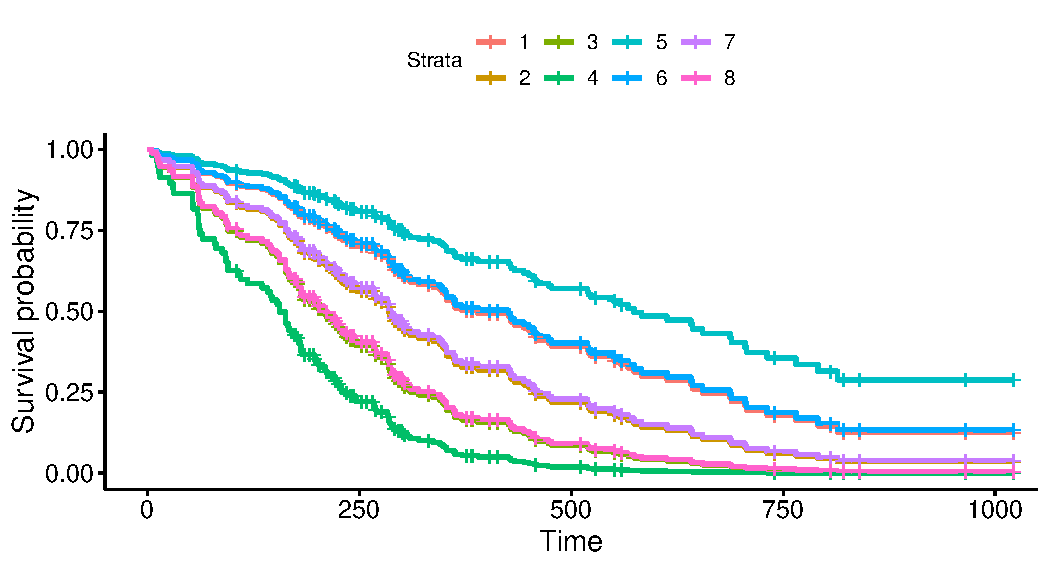
\includegraphics{figure/unnamed-chunk-155-1.pdf}
\caption{plot of chunk unnamed-chunk-155}
\end{figure}

\end{frame}

\begin{frame}[fragile]{Discussion of survival curves}
\protect\hypertarget{discussion-of-survival-curves}{}

\begin{itemize}
\item
  Best survival is teal-blue curve, stratum 5, females with
  (\texttt{ph.ecog}) score 0.
\item
  Next best: blue, stratum 6, females with score 1, and red, stratum 1,
  males score 0.
\item
  Worst: green, stratum 4, males score 3.
\item
  For any given \texttt{ph.ecog} score, females have better predicted
  survival than males.
\item
  For both genders, a lower score associated with better survival.
\end{itemize}

\end{frame}

\begin{frame}[fragile]{The coefficients in model 3}
\protect\hypertarget{the-coefficients-in-model-3}{}

\begin{Shaded}
\begin{Highlighting}[]
\KeywordTok{tidy}\NormalTok{(lung}\FloatTok{.3}\NormalTok{) }\OperatorTok\StringTok{ }\KeywordTok{select}\NormalTok{(term, estimate, p.value)}
\end{Highlighting}
\end{Shaded}

\begin{verbatim}
## # A tibble: 2 x 3
##   term    estimate  p.value
##   <chr>      <dbl>    <dbl>
## 1 sex       -0.510 0.00958 
## 2 ph.ecog    0.483 0.000266
\end{verbatim}

\begin{itemize}
\item
  \texttt{sex} coeff negative, so being higher \texttt{sex} value
  (female) goes with \emph{less} hazard of dying.
\item
  \texttt{ph.ecog} coeff positive, so higher \texttt{ph.ecog} score goes
  with \emph{more} hazard of dying
\item
  Two coeffs about same size, so being male rather than female
  corresponds to 1-point increase in \texttt{ph.ecog} score. Note how
  survival curves come in 3 pairs plus 2 odd.
\end{itemize}

\end{frame}

\begin{frame}[fragile]{Martingale residuals for this model}
\protect\hypertarget{martingale-residuals-for-this-model}{}

No problems here:

\begin{Shaded}
\begin{Highlighting}[]
\KeywordTok{ggcoxdiagnostics}\NormalTok{(lung}\FloatTok{.3}\NormalTok{) }\OperatorTok{+}\StringTok{ }\KeywordTok{geom_smooth}\NormalTok{(}\DataTypeTok{se =}\NormalTok{ F)}
\end{Highlighting}
\end{Shaded}

\begin{verbatim}
## `geom_smooth()` using method = 'loess' and formula 'y ~ x'
\end{verbatim}

\begin{figure}
\centering
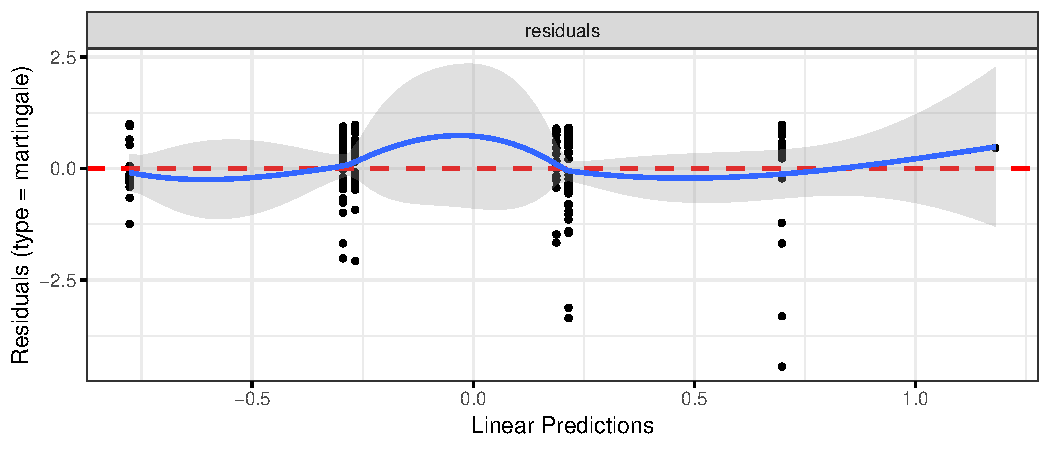
\includegraphics{figure/unnamed-chunk-157-1.pdf}
\caption{plot of chunk unnamed-chunk-157}
\end{figure}

\end{frame}

\begin{frame}[fragile]{When the Cox model fails}
\protect\hypertarget{when-the-cox-model-fails}{}

\begin{itemize}
\tightlist
\item
  Invent some data where survival is best at middling age, and worse at
  high \emph{and} low age:
\end{itemize}

\begin{Shaded}
\begin{Highlighting}[]
\NormalTok{age <-}\StringTok{ }\KeywordTok{seq}\NormalTok{(}\DecValTok{20}\NormalTok{, }\DecValTok{60}\NormalTok{, }\DecValTok{5}\NormalTok{)}
\NormalTok{survtime <-}\StringTok{ }\KeywordTok{c}\NormalTok{(}\DecValTok{10}\NormalTok{, }\DecValTok{12}\NormalTok{, }\DecValTok{11}\NormalTok{, }\DecValTok{21}\NormalTok{, }\DecValTok{15}\NormalTok{, }\DecValTok{20}\NormalTok{, }\DecValTok{8}\NormalTok{, }\DecValTok{9}\NormalTok{, }\DecValTok{11}\NormalTok{)}
\NormalTok{stat <-}\StringTok{ }\KeywordTok{c}\NormalTok{(}\DecValTok{1}\NormalTok{, }\DecValTok{1}\NormalTok{, }\DecValTok{1}\NormalTok{, }\DecValTok{1}\NormalTok{, }\DecValTok{0}\NormalTok{, }\DecValTok{1}\NormalTok{, }\DecValTok{1}\NormalTok{, }\DecValTok{1}\NormalTok{, }\DecValTok{1}\NormalTok{)}
\NormalTok{d <-}\StringTok{ }\KeywordTok{tibble}\NormalTok{(age, survtime, stat)}
\NormalTok{y <-}\StringTok{ }\KeywordTok{with}\NormalTok{(d, }\KeywordTok{Surv}\NormalTok{(survtime, stat))}
\end{Highlighting}
\end{Shaded}

\begin{itemize}
\tightlist
\item
  Small survival time 15 in middle was actually censored, so would have
  been longer if observed.
\end{itemize}

\end{frame}

\begin{frame}[fragile]{Fit Cox model}
\protect\hypertarget{fit-cox-model}{}

\footnotesize

\begin{Shaded}
\begin{Highlighting}[]
\NormalTok{y}\FloatTok{.1}\NormalTok{ <-}\StringTok{ }\KeywordTok{coxph}\NormalTok{(y }\OperatorTok{~}\StringTok{ }\NormalTok{age, }\DataTypeTok{data =}\NormalTok{ d)}
\KeywordTok{summary}\NormalTok{(y}\FloatTok{.1}\NormalTok{)}
\end{Highlighting}
\end{Shaded}

\begin{verbatim}
## Call:
## coxph(formula = y ~ age, data = d)
## 
##   n= 9, number of events= 8 
## 
##        coef exp(coef) se(coef)     z Pr(>|z|)
## age 0.01984   1.02003  0.03446 0.576    0.565
## 
##     exp(coef) exp(-coef) lower .95 upper .95
## age      1.02     0.9804    0.9534     1.091
## 
## Concordance= 0.545  (se = 0.105 )
## Likelihood ratio test= 0.33  on 1 df,   p=0.6
## Wald test            = 0.33  on 1 df,   p=0.6
## Score (logrank) test = 0.33  on 1 df,   p=0.6
\end{verbatim}

\normalsize

\end{frame}

\begin{frame}[fragile]{Martingale residuals}
\protect\hypertarget{martingale-residuals}{}

Down-and-up indicates incorrect relationship between age and survival:

\begin{Shaded}
\begin{Highlighting}[]
\KeywordTok{ggcoxdiagnostics}\NormalTok{(y}\FloatTok{.1}\NormalTok{) }\OperatorTok{+}\StringTok{ }\KeywordTok{geom_smooth}\NormalTok{(}\DataTypeTok{se =}\NormalTok{ F)}
\end{Highlighting}
\end{Shaded}

\begin{figure}
\centering
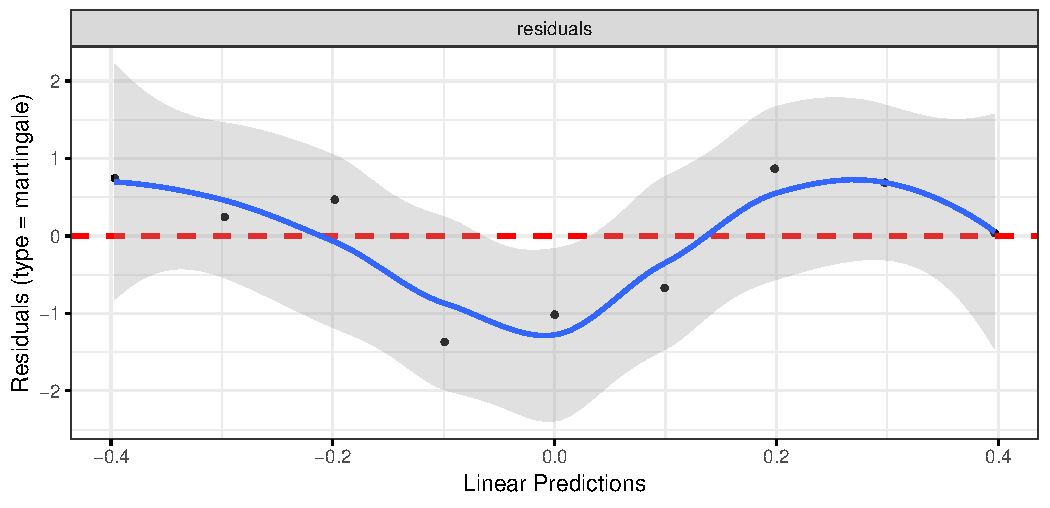
\includegraphics{figure/unnamed-chunk-160-1.pdf}
\caption{plot of chunk unnamed-chunk-160}
\end{figure}

\end{frame}

\begin{frame}[fragile]{Attempt 2}
\protect\hypertarget{attempt-2}{}

Add squared term in age:

\begin{Shaded}
\begin{Highlighting}[]
\NormalTok{y}\FloatTok{.2}\NormalTok{ <-}\StringTok{ }\KeywordTok{coxph}\NormalTok{(y }\OperatorTok{~}\StringTok{ }\NormalTok{age }\OperatorTok{+}\StringTok{ }\KeywordTok{I}\NormalTok{(age}\OperatorTok{^}\DecValTok{2}\NormalTok{), }\DataTypeTok{data =}\NormalTok{ d)}
\KeywordTok{tidy}\NormalTok{(y}\FloatTok{.2}\NormalTok{) }\OperatorTok\StringTok{ }\KeywordTok{select}\NormalTok{(term, estimate, p.value)}
\end{Highlighting}
\end{Shaded}

\begin{verbatim}
## # A tibble: 2 x 3
##   term     estimate p.value
##   <chr>       <dbl>   <dbl>
## 1 age      -0.380    0.116 
## 2 I(age^2)  0.00483  0.0977
\end{verbatim}

\begin{itemize}
\tightlist
\item
  (Marginally) helpful.
\end{itemize}

\end{frame}

\begin{frame}[fragile]{Martingale residuals this time}
\protect\hypertarget{martingale-residuals-this-time}{}

Not great, but less problematic than before:

\begin{Shaded}
\begin{Highlighting}[]
\KeywordTok{ggcoxdiagnostics}\NormalTok{(y}\FloatTok{.2}\NormalTok{) }\OperatorTok{+}\StringTok{ }\KeywordTok{geom_smooth}\NormalTok{(}\DataTypeTok{se =}\NormalTok{ F)}
\end{Highlighting}
\end{Shaded}

\begin{figure}
\centering
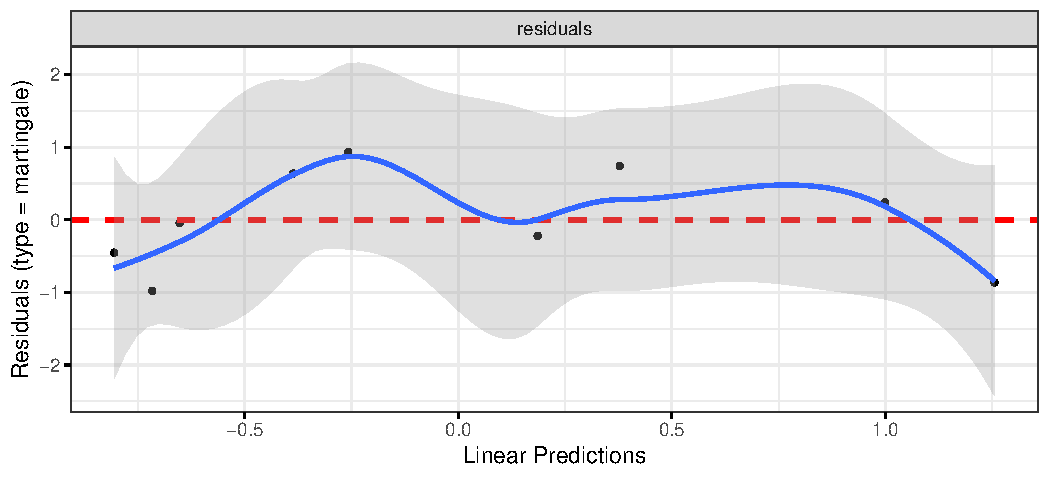
\includegraphics{figure/unnamed-chunk-162-1.pdf}
\caption{plot of chunk unnamed-chunk-162}
\end{figure}

\end{frame}

\hypertarget{analysis-of-variance}{%
\section{Analysis of variance}\label{analysis-of-variance}}

\begin{frame}{Analysis of variance}
\protect\hypertarget{analysis-of-variance-1}{}

\begin{itemize}
\item
  Analysis of variance used with:

  \begin{itemize}
  \item
    counted/measured response
  \item
    categorical explanatory variable(s)
  \item
    that is, data divided into groups, and see if response significantly
    different among groups
  \item
    or, see whether knowing group membership helps to predict response.
  \end{itemize}
\item
  Typically two stages:

  \begin{itemize}
  \item
    \(F\)-test to detect \emph{any} differences among/due to groups
  \item
    if \(F\)-test significant, do \emph{multiple comparisons} to see
    which groups significantly different from which.
  \end{itemize}
\item
  Need special multiple comparisons method because just doing (say)
  two-sample \(t\)-tests on each pair of groups gives too big a chance
  of finding ``significant'' differences by accident.
\end{itemize}

\end{frame}

\begin{frame}[fragile]{Packages}
\protect\hypertarget{packages-2}{}

These:

\begin{Shaded}
\begin{Highlighting}[]
\KeywordTok{library}\NormalTok{(tidyverse)}
\KeywordTok{library}\NormalTok{(broom)}
\KeywordTok{library}\NormalTok{(car) }\CommentTok{# for Levene's text}
\end{Highlighting}
\end{Shaded}

\end{frame}

\begin{frame}{Example: Pain threshold and hair colour}
\protect\hypertarget{example-pain-threshold-and-hair-colour}{}

\begin{itemize}
\item
  Do people with different hair colour have different abilities to deal
  with pain?
\item
  Men and women of various ages divided into 4 groups by hair colour:
  light and dark blond, light and dark brown.
\item
  Each subject given a pain sensitivity test resulting in pain threshold
  score: higher score is higher pain tolerance.
\item
  19 subjects altogether.
\end{itemize}

\end{frame}

\begin{frame}[fragile]{The data}
\protect\hypertarget{the-data-6}{}

In \texttt{hairpain.txt}:

\begin{multicols}{2}

\begin{verbatim}
hair pain
lightblond 62
lightblond 60
lightblond 71
lightblond 55
lightblond 48
darkblond 63
darkblond 57
darkblond 52
darkblond 41
darkblond 43
lightbrown 42
lightbrown 50
lightbrown 41
lightbrown 37
darkbrown 32
darkbrown 39
darkbrown 51
darkbrown 30
darkbrown 35
\end{verbatim}

\end{multicols}

\end{frame}

\begin{frame}[fragile]{Summarizing the groups}
\protect\hypertarget{summarizing-the-groups}{}

\footnotesize

\begin{Shaded}
\begin{Highlighting}[]
\NormalTok{my_url <-}\StringTok{ "http://www.utsc.utoronto.ca/~butler/d29/hairpain.txt"}
\NormalTok{hairpain <-}\StringTok{ }\KeywordTok{read_delim}\NormalTok{(my_url, }\StringTok{" "}\NormalTok{)}
\NormalTok{hairpain }\OperatorTok
\StringTok{  }\KeywordTok{group_by}\NormalTok{(hair) }\OperatorTok
\StringTok{  }\KeywordTok{summarize}\NormalTok{(}
    \DataTypeTok{n =} \KeywordTok{n}\NormalTok{(),}
    \DataTypeTok{xbar =} \KeywordTok{mean}\NormalTok{(pain),}
    \DataTypeTok{s =} \KeywordTok{sd}\NormalTok{(pain)}
\NormalTok{  )}
\end{Highlighting}
\end{Shaded}

\begin{verbatim}
## [conflicted] `summarize` found in 2 packages.
## Either pick the one you want with `::` 
## * plyr::summarize
## * dplyr::summarize
## Or declare a preference with `conflict_prefer()`
## * conflict_prefer("summarize", "plyr")
## * conflict_prefer("summarize", "dplyr")
\end{verbatim}

\normalsize

Brown-haired people seem to have lower pain tolerance.

\end{frame}

\begin{frame}[fragile]{Boxplot}
\protect\hypertarget{boxplot}{}

\begin{Shaded}
\begin{Highlighting}[]
\KeywordTok{ggplot}\NormalTok{(hairpain, }\KeywordTok{aes}\NormalTok{(}\DataTypeTok{x =}\NormalTok{ hair, }\DataTypeTok{y =}\NormalTok{ pain)) }\OperatorTok{+}\StringTok{ }\KeywordTok{geom_boxplot}\NormalTok{()}
\end{Highlighting}
\end{Shaded}

\begin{figure}
\centering
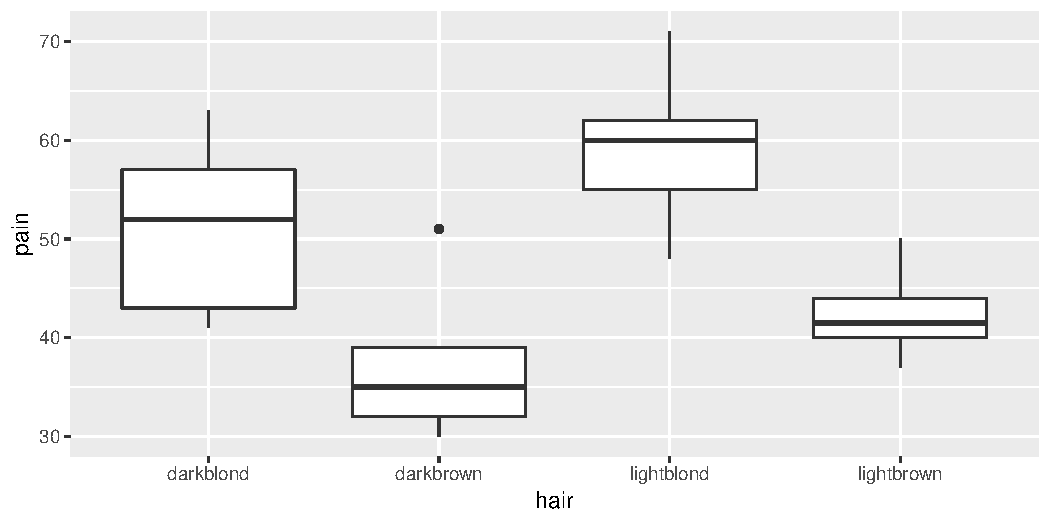
\includegraphics{figure/tartuffo-1.pdf}
\caption{plot of chunk tartuffo}
\end{figure}

\end{frame}

\begin{frame}[fragile]{Assumptions}
\protect\hypertarget{assumptions}{}

\begin{itemize}
\item
  Data should be:

  \begin{itemize}
  \item
    normally distributed within each group
  \item
    same spread for each group
  \end{itemize}
\item
  \texttt{darkbrown} group has upper outlier (suggests not normal)
\item
  \texttt{darkblond} group has smaller IQR than other groups.
\item
  But, groups \emph{small}.
\item
  Shrug shoulders and continue for moment.
\end{itemize}

\end{frame}

\begin{frame}[fragile]{Testing equality of SDs}
\protect\hypertarget{testing-equality-of-sds}{}

\begin{itemize}
\tightlist
\item
  via \textbf{Levene's test} in package \texttt{car}:
\end{itemize}

\small

\begin{Shaded}
\begin{Highlighting}[]
\KeywordTok{leveneTest}\NormalTok{(pain }\OperatorTok{~}\StringTok{ }\NormalTok{hair, }\DataTypeTok{data =}\NormalTok{ hairpain)}
\end{Highlighting}
\end{Shaded}

\begin{verbatim}
## Warning in leveneTest.default(y = y, group = group, ...): group coerced to factor.
\end{verbatim}

\begin{verbatim}
## Levene's Test for Homogeneity of Variance (center = median)
##       Df F value Pr(>F)
## group  3  0.3927   0.76
##       15
\end{verbatim}

\normalsize

\begin{itemize}
\item
  No evidence (at all) of difference among group SDs.
\item
  Possibly because groups \emph{small}.
\end{itemize}

\end{frame}

\begin{frame}[fragile]{Analysis of variance}
\protect\hypertarget{analysis-of-variance-2}{}

\small

\begin{Shaded}
\begin{Highlighting}[]
\NormalTok{hairpain}\FloatTok{.1}\NormalTok{ <-}\StringTok{ }\KeywordTok{aov}\NormalTok{(pain }\OperatorTok{~}\StringTok{ }\NormalTok{hair, }\DataTypeTok{data =}\NormalTok{ hairpain)}
\KeywordTok{summary}\NormalTok{(hairpain}\FloatTok{.1}\NormalTok{)}
\end{Highlighting}
\end{Shaded}

\begin{verbatim}
##             Df Sum Sq Mean Sq F value  Pr(>F)   
## hair         3   1361   453.6   6.791 0.00411 **
## Residuals   15   1002    66.8                   
## ---
## Signif. codes:  0 '***' 0.001 '**' 0.01 '*' 0.05 '.' 0.1 ' ' 1
\end{verbatim}

\normalsize

\begin{itemize}
\item
  P-value small: the mean pain tolerances for the four groups are
  \emph{not} all the same.
\item
  Which groups differ from which, and how?
\end{itemize}

\end{frame}

\begin{frame}{Multiple comparisons}
\protect\hypertarget{multiple-comparisons}{}

\begin{itemize}
\item
  Which groups differ from which? Multiple comparisons method. Lots.
\item
  Problem: by comparing all the groups with each other, doing many
  tests, have large chance to (possibly incorrectly) reject \(H_0:\)
  groups have equal means.
\item
  4 groups: 6 comparisons (1 vs 2, 1 vs 3, \ldots, 3 vs 4). 5 groups: 10
  comparisons. Thus 6 (or 10) chances to make mistake.
\item
  Get ``familywise error rate'' of 0.05 (whatever), no matter how many
  comparisons you're doing.
\item
  My favourite: Tukey, or ``honestly significant differences'': how far
  apart might largest, smallest group means be (if actually no
  differences). Group means more different: significantly different.
\end{itemize}

\end{frame}

\begin{frame}[fragile]{Tukey}
\protect\hypertarget{tukey}{}

\begin{itemize}
\tightlist
\item
  \texttt{TukeyHSD:}
\end{itemize}

\footnotesize

\begin{Shaded}
\begin{Highlighting}[]
\KeywordTok{TukeyHSD}\NormalTok{(hairpain}\FloatTok{.1}\NormalTok{)}
\end{Highlighting}
\end{Shaded}

\begin{verbatim}
##   Tukey multiple comparisons of means
##     95% family-wise confidence level
## 
## Fit: aov(formula = pain ~ hair, data = hairpain)
## 
## $hair
##                        diff        lwr        upr     p adj
## darkbrown-darkblond   -13.8 -28.696741  1.0967407 0.0740679
## lightblond-darkblond    8.0  -6.896741 22.8967407 0.4355768
## lightbrown-darkblond   -8.7 -24.500380  7.1003795 0.4147283
## lightblond-darkbrown   21.8   6.903259 36.6967407 0.0037079
## lightbrown-darkbrown    5.1 -10.700380 20.9003795 0.7893211
## lightbrown-lightblond -16.7 -32.500380 -0.8996205 0.0366467
\end{verbatim}

\normalsize

\end{frame}

\begin{frame}[fragile]{The old-fashioned way}
\protect\hypertarget{the-old-fashioned-way}{}

\begin{itemize}
\item
  List group means in order
\item
  Draw lines connecting groups that are \emph{not} significantly
  different:
\end{itemize}

\begin{verbatim}
darkbrown lightbrown  darkblond lightblond
37.4      42.5       51.2       59.2
-------------------------
                     ---------------
\end{verbatim}

\begin{itemize}
\item
  \texttt{lightblond} significantly higher than everything except
  \texttt{darkblond} (at \(\alpha=0.05\)).
\item
  \texttt{darkblond} in middle ground: not significantly less than
  \texttt{lightblond}, not significantly greater than \texttt{darkbrown}
  and \texttt{lightbrown}.
\item
  More data might resolve this.
\item
  Looks as if blond-haired people do have higher pain tolerance, but not
  completely clear.
\end{itemize}

\end{frame}

\begin{frame}{Some other multiple-comparison methods}
\protect\hypertarget{some-other-multiple-comparison-methods}{}

\begin{itemize}
\item
  Work any time you do \(k\) tests at once (not just ANOVA).

  \begin{itemize}
  \item
    \textbf{Bonferroni}: multiply all P-values by \(k\).
  \item
    \textbf{Holm}: multiply smallest P-value by \(k\), next-smallest by
    \(k-1\), etc.
  \item
    \textbf{False discovery rate}: multiply smallest P-value by \(k/1\),
    2nd-smallest by \(k/2\), \ldots, \(i\)-th smallest by \(k/i\).
  \end{itemize}
\item
  Stop after non-rejection.
\end{itemize}

\end{frame}

\begin{frame}{Example}
\protect\hypertarget{example}{}

\begin{itemize}
\item
  P-values 0.005, 0.015, 0.03, 0.06 (4 tests all done at once) Use
  \(\alpha=0.05\).
\item
  Bonferroni:

  \begin{itemize}
  \item
    Multiply all P-values by 4 (4 tests).
  \item
    Reject only 1st null.
  \end{itemize}
\item
  Holm:

  \begin{itemize}
  \item
    Times smallest P-value by 4: \(0.005*4=0.020<0.05\), reject.
  \item
    Times next smallest by 3: \(0.015*3=0.045<0.05\), reject.
  \item
    Times next smallest by 2: \(0.03*2=0.06>0.05\), do not reject. Stop.
  \end{itemize}
\end{itemize}

\end{frame}

\begin{frame}{\ldots Continued}
\protect\hypertarget{continued}{}

\begin{itemize}
\item
  With P-values 0.005, 0.015, 0.03, 0.06:
\item
  False discovery rate:

  \begin{itemize}
  \item
    Times smallest P-value by 4: \(0.005*4=0.02<0.05\): reject.
  \item
    Times second smallest by \(4/2\): \(0.015*4/2=0.03<0.05\), reject.
  \item
    Times third smallest by \(4/3\): \(0.03*4/3=0.04<0.05\), reject.
  \item
    Times fourth smallest by \(4/4\): \(0.06*4/4=0.06>0.05\), do not
    reject. Stop.
  \end{itemize}
\end{itemize}

\end{frame}

\begin{frame}[fragile]{\texttt{pairwise.t.test}}
\protect\hypertarget{pairwise.t.test}{}

\tiny

\begin{Shaded}
\begin{Highlighting}[]
\KeywordTok{attach}\NormalTok{(hairpain)}
\KeywordTok{pairwise.t.test}\NormalTok{(pain, hair, }\DataTypeTok{p.adj =} \StringTok{"none"}\NormalTok{)}
\end{Highlighting}
\end{Shaded}

\begin{verbatim}
## 
##  Pairwise comparisons using t tests with pooled SD 
## 
## data:  pain and hair 
## 
##            darkblond darkbrown lightblond
## darkbrown  0.01748   -         -         
## lightblond 0.14251   0.00075   -         
## lightbrown 0.13337   0.36695   0.00817   
## 
## P value adjustment method: none
\end{verbatim}

\begin{Shaded}
\begin{Highlighting}[]
\KeywordTok{pairwise.t.test}\NormalTok{(pain, hair, }\DataTypeTok{p.adj =} \StringTok{"holm"}\NormalTok{)}
\end{Highlighting}
\end{Shaded}

\begin{verbatim}
## 
##  Pairwise comparisons using t tests with pooled SD 
## 
## data:  pain and hair 
## 
##            darkblond darkbrown lightblond
## darkbrown  0.0699    -         -         
## lightblond 0.4001    0.0045    -         
## lightbrown 0.4001    0.4001    0.0408    
## 
## P value adjustment method: holm
\end{verbatim}

\normalsize

\end{frame}

\begin{frame}[fragile]{\texttt{pairwise.t.test} part 2}
\protect\hypertarget{pairwise.t.test-part-2}{}

\tiny

\begin{Shaded}
\begin{Highlighting}[]
\KeywordTok{pairwise.t.test}\NormalTok{(pain, hair, }\DataTypeTok{p.adj =} \StringTok{"fdr"}\NormalTok{)}
\end{Highlighting}
\end{Shaded}

\begin{verbatim}
## 
##  Pairwise comparisons using t tests with pooled SD 
## 
## data:  pain and hair 
## 
##            darkblond darkbrown lightblond
## darkbrown  0.0350    -         -         
## lightblond 0.1710    0.0045    -         
## lightbrown 0.1710    0.3670    0.0245    
## 
## P value adjustment method: fdr
\end{verbatim}

\begin{Shaded}
\begin{Highlighting}[]
\KeywordTok{pairwise.t.test}\NormalTok{(pain, hair, }\DataTypeTok{p.adj =} \StringTok{"bon"}\NormalTok{)}
\end{Highlighting}
\end{Shaded}

\begin{verbatim}
## 
##  Pairwise comparisons using t tests with pooled SD 
## 
## data:  pain and hair 
## 
##            darkblond darkbrown lightblond
## darkbrown  0.1049    -         -         
## lightblond 0.8550    0.0045    -         
## lightbrown 0.8002    1.0000    0.0490    
## 
## P value adjustment method: bonferroni
\end{verbatim}

\normalsize

\end{frame}

\begin{frame}{Comments}
\protect\hypertarget{comments-15}{}

\begin{itemize}
\item
  P-values all adjusted upwards from ``none''.
\item
  Required because 6 tests at once.
\item
  Highest P-values for Bonferroni: most ``conservative''.
\item
  Prefer Tukey or FDR or Holm.
\item
  Tukey only applies to ANOVA, not to other cases of multiple testing.
\end{itemize}

\end{frame}

\begin{frame}[fragile]{Rats and vitamin B}
\protect\hypertarget{rats-and-vitamin-b}{}

\begin{itemize}
\item
  What is the effect of dietary vitamin B on the kidney?
\item
  A number of rats were randomized to receive either a B-supplemented
  diet or a regular diet.
\item
  Desired to control for initial size of rats, so classified into size
  classes \texttt{lean} and \texttt{obese}.
\item
  After 20 weeks, rats' kidneys weighed.
\item
  Variables:

  \begin{itemize}
  \item
    Response: \texttt{kidneyweight} (grams).
  \item
    Explanatory: \texttt{diet}, \texttt{ratsize}.
  \end{itemize}
\item
  Read in data:
\end{itemize}

\begin{Shaded}
\begin{Highlighting}[]
\NormalTok{my_url <-}\StringTok{ "http://www.utsc.utoronto.ca/~butler/d29/vitaminb.txt"}
\NormalTok{vitaminb <-}\StringTok{ }\KeywordTok{read_delim}\NormalTok{(my_url, }\StringTok{" "}\NormalTok{)}
\end{Highlighting}
\end{Shaded}

\begin{verbatim}
## Parsed with column specification:
## cols(
##   ratsize = col_character(),
##   diet = col_character(),
##   kidneyweight = col_double()
## )
\end{verbatim}

\end{frame}

\begin{frame}[fragile]{The data}
\protect\hypertarget{the-data-7}{}

\begin{Shaded}
\begin{Highlighting}[]
\NormalTok{vitaminb}
\end{Highlighting}
\end{Shaded}

\begin{verbatim}
## # A tibble: 28 x 3
##    ratsize diet     kidneyweight
##    <chr>   <chr>           <dbl>
##  1 lean    regular          1.62
##  2 lean    regular          1.8 
##  3 lean    regular          1.71
##  4 lean    regular          1.81
##  5 lean    regular          1.47
##  6 lean    regular          1.37
##  7 lean    regular          1.71
##  8 lean    vitaminb         1.51
##  9 lean    vitaminb         1.65
## 10 lean    vitaminb         1.45
## # … with 18 more rows
\end{verbatim}

\end{frame}

\begin{frame}[fragile]{Grouped boxplot}
\protect\hypertarget{grouped-boxplot}{}

\begin{Shaded}
\begin{Highlighting}[]
\KeywordTok{ggplot}\NormalTok{(vitaminb, }\KeywordTok{aes}\NormalTok{(}
  \DataTypeTok{x =}\NormalTok{ ratsize, }\DataTypeTok{y =}\NormalTok{ kidneyweight,}
  \DataTypeTok{fill =}\NormalTok{ diet}
\NormalTok{)) }\OperatorTok{+}\StringTok{ }\KeywordTok{geom_boxplot}\NormalTok{()}
\end{Highlighting}
\end{Shaded}

\begin{figure}
\centering
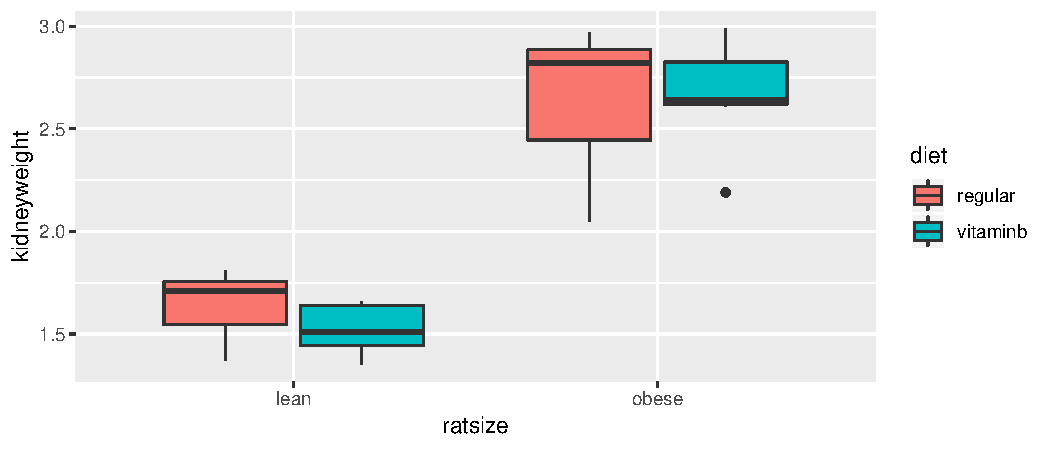
\includegraphics{figure/unnamed-chunk-172-1.pdf}
\caption{plot of chunk unnamed-chunk-172}
\end{figure}

\end{frame}

\begin{frame}[fragile]{What's going on?}
\protect\hypertarget{whats-going-on}{}

\begin{itemize}
\tightlist
\item
  Calculate group means:
\end{itemize}

\footnotesize

\begin{Shaded}
\begin{Highlighting}[]
\NormalTok{summary <-}\StringTok{ }\NormalTok{vitaminb }\OperatorTok
\StringTok{  }\KeywordTok{group_by}\NormalTok{(ratsize, diet) }\OperatorTok
\StringTok{  }\KeywordTok{summarize}\NormalTok{(}\DataTypeTok{mean =} \KeywordTok{mean}\NormalTok{(kidneyweight))}
\end{Highlighting}
\end{Shaded}

\begin{verbatim}
## [conflicted] `summarize` found in 2 packages.
## Either pick the one you want with `::` 
## * plyr::summarize
## * dplyr::summarize
## Or declare a preference with `conflict_prefer()`
## * conflict_prefer("summarize", "plyr")
## * conflict_prefer("summarize", "dplyr")
\end{verbatim}

\begin{Shaded}
\begin{Highlighting}[]
\NormalTok{summary}
\end{Highlighting}
\end{Shaded}

\begin{verbatim}
## function (object, ...) 
## UseMethod("summary")
## <bytecode: 0x561d8d5b3e20>
## <environment: namespace:base>
\end{verbatim}

\normalsize

\begin{itemize}
\item
  Rat size: a large and consistent effect.
\item
  Diet: small/no effect (compare same rat size, different diet).
\item
  Effect of rat size \emph{same} for each diet: no interaction.
\end{itemize}

\end{frame}

\begin{frame}[fragile]{ANOVA with interaction}
\protect\hypertarget{anova-with-interaction}{}

\begin{Shaded}
\begin{Highlighting}[]
\NormalTok{vitaminb}\FloatTok{.1}\NormalTok{ <-}\StringTok{ }\KeywordTok{aov}\NormalTok{(kidneyweight }\OperatorTok{~}\StringTok{ }\NormalTok{ratsize }\OperatorTok{*}\StringTok{ }\NormalTok{diet,}
  \DataTypeTok{data =}\NormalTok{ vitaminb}
\NormalTok{)}
\KeywordTok{summary}\NormalTok{(vitaminb}\FloatTok{.1}\NormalTok{)}
\end{Highlighting}
\end{Shaded}

\begin{verbatim}
##              Df Sum Sq Mean Sq F value   Pr(>F)    
## ratsize       1  8.068   8.068 141.179 1.53e-11 ***
## diet          1  0.012   0.012   0.218    0.645    
## ratsize:diet  1  0.036   0.036   0.638    0.432    
## Residuals    24  1.372   0.057                     
## ---
## Signif. codes:  0 '***' 0.001 '**' 0.01 '*' 0.05 '.' 0.1 ' ' 1
\end{verbatim}

\begin{itemize}
\tightlist
\item
  Significance/nonsignificance as we expected.
\item
  Note no significant interaction (can be removed).
\end{itemize}

\end{frame}

\begin{frame}[fragile]{Interaction plot}
\protect\hypertarget{interaction-plot}{}

\begin{itemize}
\tightlist
\item
  Plot mean of response variable against one of the explanatory, using
  other one as groups. Start from \texttt{summary}:
\end{itemize}

\begin{Shaded}
\begin{Highlighting}[]
\NormalTok{g <-}\StringTok{ }\KeywordTok{ggplot}\NormalTok{(summary, }\KeywordTok{aes}\NormalTok{(}
  \DataTypeTok{x =}\NormalTok{ ratsize, }\DataTypeTok{y =}\NormalTok{ mean,}
  \DataTypeTok{colour =}\NormalTok{ diet, }\DataTypeTok{group =}\NormalTok{ diet}
\NormalTok{)) }\OperatorTok{+}
\StringTok{  }\KeywordTok{geom_point}\NormalTok{() }\OperatorTok{+}\StringTok{ }\KeywordTok{geom_line}\NormalTok{()}
\end{Highlighting}
\end{Shaded}

\begin{verbatim}
## Error: You're passing a function as global data.
## Have you misspelled the `data` argument in `ggplot()`
\end{verbatim}

\begin{itemize}
\tightlist
\item
  For this, have to give \emph{both} \texttt{group} and \texttt{colour}.
\end{itemize}

\end{frame}

\begin{frame}[fragile]{The interaction plot}
\protect\hypertarget{the-interaction-plot}{}

\begin{Shaded}
\begin{Highlighting}[]
\NormalTok{g}
\end{Highlighting}
\end{Shaded}

\begin{figure}
\centering
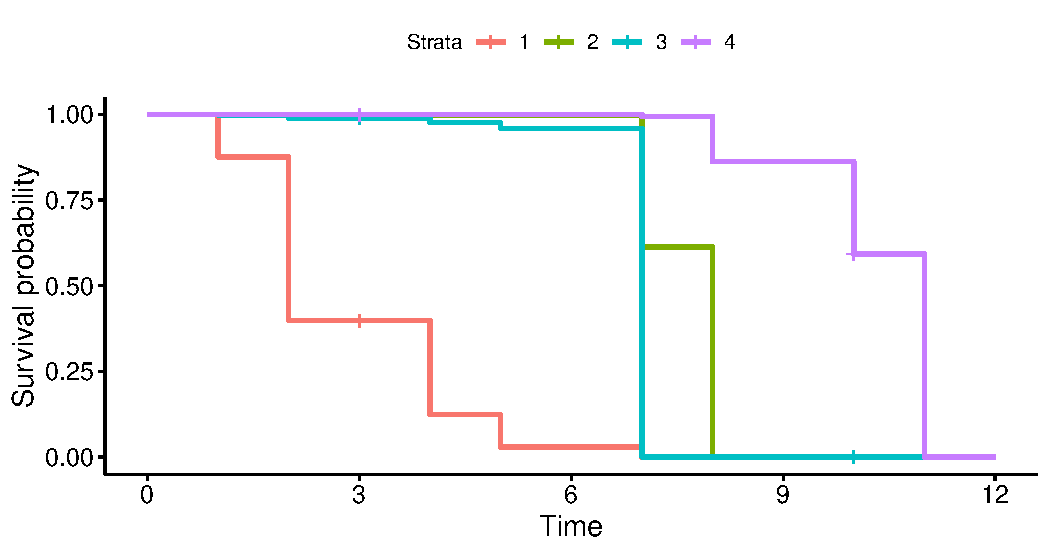
\includegraphics{figure/unnamed-chunk-176-1.pdf}
\caption{plot of chunk unnamed-chunk-176}
\end{figure}

Lines basically parallel, indicating no interaction.

\end{frame}

\begin{frame}[fragile]{Take out interaction}
\protect\hypertarget{take-out-interaction}{}

\small

\begin{Shaded}
\begin{Highlighting}[]
\NormalTok{vitaminb}\FloatTok{.2}\NormalTok{ <-}\StringTok{ }\KeywordTok{update}\NormalTok{(vitaminb}\FloatTok{.1}\NormalTok{, . }\OperatorTok{~}\StringTok{ }\NormalTok{. }\OperatorTok{-}\StringTok{ }\NormalTok{ratsize}\OperatorTok{:}\NormalTok{diet)}
\KeywordTok{summary}\NormalTok{(vitaminb}\FloatTok{.2}\NormalTok{)}
\end{Highlighting}
\end{Shaded}

\begin{verbatim}
##             Df Sum Sq Mean Sq F value   Pr(>F)    
## ratsize      1  8.068   8.068 143.256 7.59e-12 ***
## diet         1  0.012   0.012   0.221    0.643    
## Residuals   25  1.408   0.056                     
## ---
## Signif. codes:  0 '***' 0.001 '**' 0.01 '*' 0.05 '.' 0.1 ' ' 1
\end{verbatim}

\normalsize

\begin{itemize}
\item
  No Tukey for \texttt{diet}: not significant.
\item
  No Tukey for \texttt{ratsize}: only two sizes, and already know that
  obese rats have larger kidneys than lean ones.
\item
  Bottom line: diet has no effect on kidney size once you control for
  size of rat.
\end{itemize}

\end{frame}

\begin{frame}[fragile]{The auto noise data}
\protect\hypertarget{the-auto-noise-data}{}

In 1973, the President of Texaco cited an automobile filter developed by
Associated Octel Company as effective in reducing pollution. However,
questions had been raised about the effects of filter silencing. He
referred to the data included in the report (and below) as evidence that
the silencing properties of the Octel filter were at least equal to
those of standard silencers.

\begin{Shaded}
\begin{Highlighting}[]
\NormalTok{u <-}\StringTok{ "http://www.utsc.utoronto.ca/~butler/d29/autonoise.txt"}
\NormalTok{autonoise <-}\StringTok{ }\KeywordTok{read_table}\NormalTok{(u)}
\end{Highlighting}
\end{Shaded}

\begin{verbatim}
## Parsed with column specification:
## cols(
##   noise = col_double(),
##   size = col_character(),
##   type = col_character(),
##   side = col_character()
## )
\end{verbatim}

\end{frame}

\begin{frame}[fragile]{The data}
\protect\hypertarget{the-data-8}{}

\begin{Shaded}
\begin{Highlighting}[]
\NormalTok{autonoise}
\end{Highlighting}
\end{Shaded}

\begin{verbatim}
## # A tibble: 36 x 4
##    noise size  type  side 
##    <dbl> <chr> <chr> <chr>
##  1   840 M     Std   R    
##  2   770 L     Octel L    
##  3   820 M     Octel R    
##  4   775 L     Octel R    
##  5   825 M     Octel L    
##  6   840 M     Std   R    
##  7   845 M     Std   L    
##  8   825 M     Octel L    
##  9   815 M     Octel L    
## 10   845 M     Std   R    
## # … with 26 more rows
\end{verbatim}

\end{frame}

\begin{frame}[fragile]{Making boxplot}
\protect\hypertarget{making-boxplot}{}

\begin{itemize}
\item
  Make a boxplot, but have combinations of filter type and engine size.
\item
  Use grouped boxplot again, thus:
\end{itemize}

\begin{Shaded}
\begin{Highlighting}[]
\NormalTok{g <-}\StringTok{ }\NormalTok{autonoise }\OperatorTok
\StringTok{  }\KeywordTok{ggplot}\NormalTok{(}\KeywordTok{aes}\NormalTok{(}\DataTypeTok{x =}\NormalTok{ size, }\DataTypeTok{y =}\NormalTok{ noise, }\DataTypeTok{fill =}\NormalTok{ type)) }\OperatorTok{+}
\StringTok{  }\KeywordTok{geom_boxplot}\NormalTok{()}
\end{Highlighting}
\end{Shaded}

\end{frame}

\begin{frame}[fragile]{The boxplot}
\protect\hypertarget{the-boxplot}{}

\begin{itemize}
\item
  See difference in engine noise between Octel and standard is larger
  for medium engine size than for large or small.
\item
  Some evidence of differences in spreads (ignore for now):
\end{itemize}

\begin{Shaded}
\begin{Highlighting}[]
\NormalTok{g}
\end{Highlighting}
\end{Shaded}

\begin{figure}
\centering
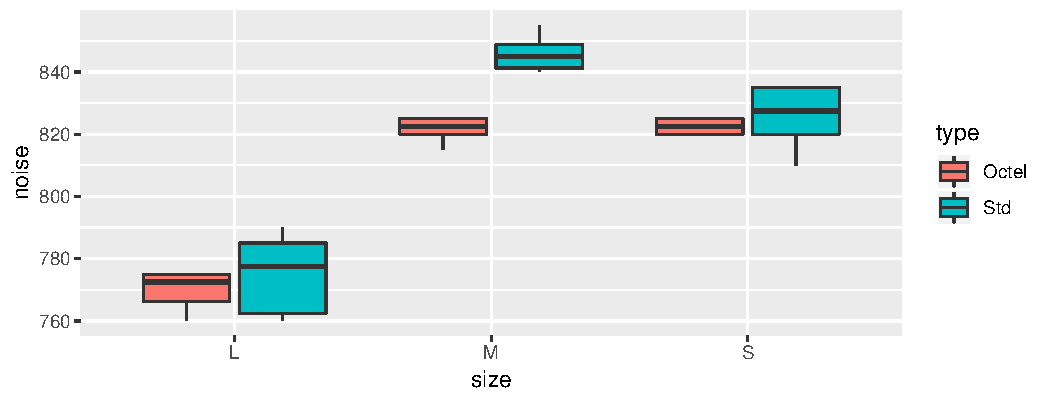
\includegraphics{figure/unnamed-chunk-181-1.pdf}
\caption{plot of chunk unnamed-chunk-181}
\end{figure}

\end{frame}

\begin{frame}[fragile]{ANOVA}
\protect\hypertarget{anova}{}

\small

\begin{Shaded}
\begin{Highlighting}[]
\NormalTok{autonoise}\FloatTok{.1}\NormalTok{ <-}\StringTok{ }\KeywordTok{aov}\NormalTok{(noise }\OperatorTok{~}\StringTok{ }\NormalTok{size }\OperatorTok{*}\StringTok{ }\NormalTok{type, }\DataTypeTok{data =}\NormalTok{ autonoise)}
\KeywordTok{summary}\NormalTok{(autonoise}\FloatTok{.1}\NormalTok{)}
\end{Highlighting}
\end{Shaded}

\begin{verbatim}
##             Df Sum Sq Mean Sq F value   Pr(>F)    
## size         2  26051   13026 199.119  < 2e-16 ***
## type         1   1056    1056  16.146 0.000363 ***
## size:type    2    804     402   6.146 0.005792 ** 
## Residuals   30   1962      65                     
## ---
## Signif. codes:  0 '***' 0.001 '**' 0.01 '*' 0.05 '.' 0.1 ' ' 1
\end{verbatim}

\normalsize

\begin{itemize}
\item
  The interaction is significant, as we suspected from the boxplots.
\item
  The within-group spreads don't look very equal, but only based on 6
  obs each.
\end{itemize}

\end{frame}

\begin{frame}[fragile]{Tukey: ouch!}
\protect\hypertarget{tukey-ouch}{}

\scriptsize

\begin{Shaded}
\begin{Highlighting}[]
\NormalTok{autonoise}\FloatTok{.2}\NormalTok{ <-}\StringTok{ }\KeywordTok{TukeyHSD}\NormalTok{(autonoise}\FloatTok{.1}\NormalTok{)}
\NormalTok{autonoise}\FloatTok{.2}\OperatorTok{$}\StringTok{`}\DataTypeTok{size:type}\StringTok{`}
\end{Highlighting}
\end{Shaded}

\begin{verbatim}
##                        diff        lwr        upr        p adj
## M:Octel-L:Octel  51.6666667  37.463511  65.869823 6.033496e-11
## S:Octel-L:Octel  52.5000000  38.296844  66.703156 4.089762e-11
## L:Std-L:Octel     5.0000000  -9.203156  19.203156 8.890358e-01
## M:Std-L:Octel    75.8333333  61.630177  90.036489 4.962697e-14
## S:Std-L:Octel    55.8333333  41.630177  70.036489 9.002910e-12
## S:Octel-M:Octel   0.8333333 -13.369823  15.036489 9.999720e-01
## L:Std-M:Octel   -46.6666667 -60.869823 -32.463511 6.766649e-10
## M:Std-M:Octel    24.1666667   9.963511  38.369823 1.908995e-04
## S:Std-M:Octel     4.1666667 -10.036489  18.369823 9.454142e-01
## L:Std-S:Octel   -47.5000000 -61.703156 -33.296844 4.477636e-10
## M:Std-S:Octel    23.3333333   9.130177  37.536489 3.129974e-04
## S:Std-S:Octel     3.3333333 -10.869823  17.536489 9.787622e-01
## M:Std-L:Std      70.8333333  56.630177  85.036489 6.583623e-14
## S:Std-L:Std      50.8333333  36.630177  65.036489 8.937329e-11
## S:Std-M:Std     -20.0000000 -34.203156  -5.796844 2.203265e-03
\end{verbatim}

\normalsize

\end{frame}

\begin{frame}[fragile]{Interaction plot}
\protect\hypertarget{interaction-plot-1}{}

\begin{itemize}
\item
  This time, don't have summary of mean noise for each size-type
  combination.
\item
  One way is to compute summaries (means) first, and feed into
  \texttt{ggplot} as in vitamin B example.
\item
  Or, have \texttt{ggplot} compute them for us, thus:
\end{itemize}

\begin{Shaded}
\begin{Highlighting}[]
\NormalTok{g <-}\StringTok{ }\KeywordTok{ggplot}\NormalTok{(autonoise, }\KeywordTok{aes}\NormalTok{(}
  \DataTypeTok{x =}\NormalTok{ size, }\DataTypeTok{y =}\NormalTok{ noise,}
  \DataTypeTok{colour =}\NormalTok{ type, }\DataTypeTok{group =}\NormalTok{ type}
\NormalTok{)) }\OperatorTok{+}
\StringTok{  }\KeywordTok{stat_summary}\NormalTok{(}\DataTypeTok{fun.y =}\NormalTok{ mean, }\DataTypeTok{geom =} \StringTok{"point"}\NormalTok{) }\OperatorTok{+}
\StringTok{  }\KeywordTok{stat_summary}\NormalTok{(}\DataTypeTok{fun.y =}\NormalTok{ mean, }\DataTypeTok{geom =} \StringTok{"line"}\NormalTok{)}
\end{Highlighting}
\end{Shaded}

\end{frame}

\begin{frame}[fragile]{Interaction plot}
\protect\hypertarget{interaction-plot-2}{}

The lines are definitely \emph{not} parallel, showing that the effect of
\texttt{type} is different for medium-sized engines than for others:

\begin{Shaded}
\begin{Highlighting}[]
\NormalTok{g}
\end{Highlighting}
\end{Shaded}

\begin{figure}
\centering
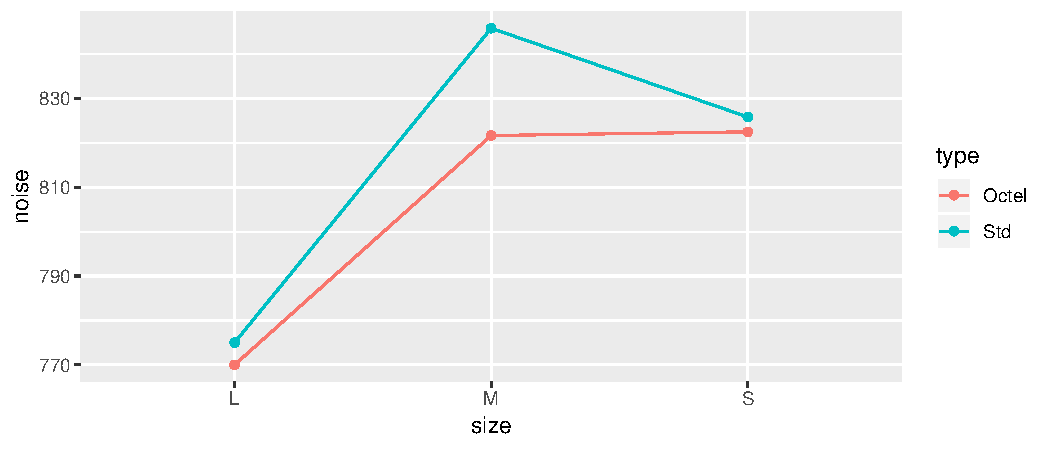
\includegraphics{figure/unnamed-chunk-185-1.pdf}
\caption{plot of chunk unnamed-chunk-185}
\end{figure}

\end{frame}

\begin{frame}[fragile]{If you don't like that\ldots}
\protect\hypertarget{if-you-dont-like-that}{}

\ldots then compute the means first, in a pipeline:

\footnotesize

\begin{Shaded}
\begin{Highlighting}[]
\NormalTok{autonoise }\OperatorTok
\StringTok{  }\KeywordTok{group_by}\NormalTok{(size, type) }\OperatorTok
\StringTok{  }\KeywordTok{summarize}\NormalTok{(}\DataTypeTok{mean_noise =} \KeywordTok{mean}\NormalTok{(noise)) }\OperatorTok
\StringTok{  }\KeywordTok{ggplot}\NormalTok{(}\KeywordTok{aes}\NormalTok{(}
    \DataTypeTok{x =}\NormalTok{ size, }\DataTypeTok{y =}\NormalTok{ mean_noise, }\DataTypeTok{group =}\NormalTok{ type,}
    \DataTypeTok{colour =}\NormalTok{ type}
\NormalTok{  )) }\OperatorTok{+}\StringTok{ }\KeywordTok{geom_point}\NormalTok{() }\OperatorTok{+}\StringTok{ }\KeywordTok{geom_line}\NormalTok{()}
\end{Highlighting}
\end{Shaded}

\begin{verbatim}
## [conflicted] `summarize` found in 2 packages.
## Either pick the one you want with `::` 
## * plyr::summarize
## * dplyr::summarize
## Or declare a preference with `conflict_prefer()`
## * conflict_prefer("summarize", "plyr")
## * conflict_prefer("summarize", "dplyr")
\end{verbatim}

\normalsize

\end{frame}

\begin{frame}{Simple effects for auto noise example}
\protect\hypertarget{simple-effects-for-auto-noise-example}{}

\begin{itemize}
\item
  In auto noise example, weren't interested in all comparisons between
  car size and filter type combinations.
\item
  Wanted to demonstrate (lack of) difference between filter types
  \emph{for each car type}.
\item
  These are called \textbf{simple effects} of one variable (filter type)
  conditional on other variable (car type).
\item
  To do this, pull out just the data for small cars, compare noise for
  the two filter types. Then repeat for medium and large cars. (Three
  one-way ANOVAs.)
\end{itemize}

\end{frame}

\begin{frame}[fragile]{Do it using \texttt{dplyr\ tools}}
\protect\hypertarget{do-it-using-dplyr-tools}{}

\begin{itemize}
\tightlist
\item
  Small cars:
\end{itemize}

\begin{Shaded}
\begin{Highlighting}[]
\NormalTok{autonoise }\OperatorTok
\StringTok{  }\KeywordTok{filter}\NormalTok{(size }\OperatorTok{==}\StringTok{ "S"}\NormalTok{) }\OperatorTok
\StringTok{  }\KeywordTok{aov}\NormalTok{(noise }\OperatorTok{~}\StringTok{ }\NormalTok{type, }\DataTypeTok{data =}\NormalTok{ .) }\OperatorTok
\StringTok{  }\KeywordTok{summary}\NormalTok{()}
\end{Highlighting}
\end{Shaded}

\begin{verbatim}
##             Df Sum Sq Mean Sq F value Pr(>F)
## type         1   33.3   33.33   0.548  0.476
## Residuals   10  608.3   60.83
\end{verbatim}

\begin{itemize}
\item
  No filter difference for small cars.
\item
  For Medium, change \texttt{S} to \texttt{M} and repeat.
\end{itemize}

\end{frame}

\begin{frame}[fragile]{Simple effect of filter type for medium cars}
\protect\hypertarget{simple-effect-of-filter-type-for-medium-cars}{}

\{\small

\begin{Shaded}
\begin{Highlighting}[]
\NormalTok{autonoise }\OperatorTok
\StringTok{  }\KeywordTok{filter}\NormalTok{(size }\OperatorTok{==}\StringTok{ "M"}\NormalTok{) }\OperatorTok
\StringTok{  }\KeywordTok{aov}\NormalTok{(noise }\OperatorTok{~}\StringTok{ }\NormalTok{type, }\DataTypeTok{data =}\NormalTok{ .) }\OperatorTok
\StringTok{  }\KeywordTok{summary}\NormalTok{()}
\end{Highlighting}
\end{Shaded}

\begin{verbatim}
##             Df Sum Sq Mean Sq F value   Pr(>F)    
## type         1 1752.1  1752.1   68.93 8.49e-06 ***
## Residuals   10  254.2    25.4                     
## ---
## Signif. codes:  0 '***' 0.001 '**' 0.01 '*' 0.05 '.' 0.1 ' ' 1
\end{verbatim}

\}

\begin{itemize}
\tightlist
\item
  There \emph{is} an effect of filter type for medium cars. Look at
  means to investigate (over).
\end{itemize}

\end{frame}

\begin{frame}[fragile]{Mean noise for each filter type}
\protect\hypertarget{mean-noise-for-each-filter-type}{}

\ldots for medium engine size:

\begin{Shaded}
\begin{Highlighting}[]
\NormalTok{autonoise }\OperatorTok
\StringTok{  }\KeywordTok{filter}\NormalTok{(size }\OperatorTok{==}\StringTok{ "M"}\NormalTok{) }\OperatorTok
\StringTok{  }\KeywordTok{group_by}\NormalTok{(type) }\OperatorTok
\StringTok{  }\KeywordTok{summarize}\NormalTok{(}\DataTypeTok{m =} \KeywordTok{mean}\NormalTok{(noise))}
\end{Highlighting}
\end{Shaded}

\begin{verbatim}
## [conflicted] `summarize` found in 2 packages.
## Either pick the one you want with `::` 
## * plyr::summarize
## * dplyr::summarize
## Or declare a preference with `conflict_prefer()`
## * conflict_prefer("summarize", "plyr")
## * conflict_prefer("summarize", "dplyr")
\end{verbatim}

\begin{itemize}
\tightlist
\item
  Octel filters produce \emph{less} noise for medium cars.
\end{itemize}

\end{frame}

\begin{frame}[fragile]{Large cars}
\protect\hypertarget{large-cars}{}

\begin{itemize}
\tightlist
\item
  Large cars:
\end{itemize}

\begin{Shaded}
\begin{Highlighting}[]
\NormalTok{autonoise }\OperatorTok
\StringTok{  }\KeywordTok{filter}\NormalTok{(size }\OperatorTok{==}\StringTok{ "L"}\NormalTok{) }\OperatorTok
\StringTok{  }\KeywordTok{aov}\NormalTok{(noise }\OperatorTok{~}\StringTok{ }\NormalTok{type, }\DataTypeTok{data =}\NormalTok{ .) }\OperatorTok
\StringTok{  }\KeywordTok{summary}\NormalTok{()}
\end{Highlighting}
\end{Shaded}

\begin{verbatim}
##             Df Sum Sq Mean Sq F value Pr(>F)
## type         1     75      75   0.682  0.428
## Residuals   10   1100     110
\end{verbatim}

\begin{itemize}
\tightlist
\item
  No significant difference again.
\end{itemize}

\end{frame}

\begin{frame}[fragile]{Or\ldots }
\protect\hypertarget{or}{}

use \texttt{glance} from \texttt{broom}:

\small

\begin{Shaded}
\begin{Highlighting}[]
\NormalTok{autonoise }\OperatorTok
\StringTok{  }\KeywordTok{filter}\NormalTok{(size }\OperatorTok{==}\StringTok{ "L"}\NormalTok{) }\OperatorTok
\StringTok{  }\KeywordTok{aov}\NormalTok{(noise }\OperatorTok{~}\StringTok{ }\NormalTok{type, }\DataTypeTok{data =}\NormalTok{ .) }\OperatorTok
\StringTok{  }\KeywordTok{glance}\NormalTok{()}
\end{Highlighting}
\end{Shaded}

\begin{verbatim}
## # A tibble: 1 x 11
##   r.squared adj.r.squared sigma statistic p.value    df
##       <dbl>         <dbl> <dbl>     <dbl>   <dbl> <int>
## 1    0.0638       -0.0298  10.5     0.682   0.428     2
## # … with 5 more variables: logLik <dbl>, AIC <dbl>,
## #   BIC <dbl>, deviance <dbl>, df.residual <int>
\end{verbatim}

\normalsize

\begin{itemize}
\tightlist
\item
  P-value same as from \texttt{summary} output.
\end{itemize}

\end{frame}

\begin{frame}[fragile]{All at once, using split/apply/combine}
\protect\hypertarget{all-at-once-using-splitapplycombine}{}

The ``split'' part:

\begin{Shaded}
\begin{Highlighting}[]
\NormalTok{autonoise }\OperatorTok
\StringTok{  }\KeywordTok{group_by}\NormalTok{(size) }\OperatorTok
\StringTok{  }\KeywordTok{nest}\NormalTok{()}
\end{Highlighting}
\end{Shaded}

\begin{verbatim}
## # A tibble: 3 x 2
##   size  data             
##   <chr> <list>           
## 1 M     <tibble [12 × 3]>
## 2 L     <tibble [12 × 3]>
## 3 S     <tibble [12 × 3]>
\end{verbatim}

Now have \emph{three} rows, with the data frame for each size encoded as
\emph{one element} of this data frame.

\end{frame}

\begin{frame}[fragile]{Apply}
\protect\hypertarget{apply}{}

\begin{itemize}
\tightlist
\item
  Write function to do \texttt{aov} on a data frame with columns
  \texttt{noise} and \texttt{type}, returning P-value:
\end{itemize}

\begin{Shaded}
\begin{Highlighting}[]
\NormalTok{aov_pval <-}\StringTok{ }\ControlFlowTok{function}\NormalTok{(x) \{}
\NormalTok{  noise}\FloatTok{.1}\NormalTok{ <-}\StringTok{ }\KeywordTok{aov}\NormalTok{(noise }\OperatorTok{~}\StringTok{ }\NormalTok{type, }\DataTypeTok{data =}\NormalTok{ x)}
\NormalTok{  gg <-}\StringTok{ }\KeywordTok{glance}\NormalTok{(noise}\FloatTok{.1}\NormalTok{)}
\NormalTok{  gg}\OperatorTok{$}\NormalTok{p.value}
\NormalTok{\}}
\end{Highlighting}
\end{Shaded}

\begin{itemize}
\tightlist
\item
  Test it:
\end{itemize}

\begin{Shaded}
\begin{Highlighting}[]
\NormalTok{autonoise }\OperatorTok
\StringTok{  }\KeywordTok{filter}\NormalTok{(size }\OperatorTok{==}\StringTok{ "L"}\NormalTok{) }\OperatorTok
\StringTok{  }\KeywordTok{aov_pval}\NormalTok{()}
\end{Highlighting}
\end{Shaded}

\begin{verbatim}
## [1] 0.428221
\end{verbatim}

\begin{itemize}
\tightlist
\item
  Check.
\end{itemize}

\end{frame}

\begin{frame}[fragile]{Combine}
\protect\hypertarget{combine}{}

\begin{itemize}
\tightlist
\item
  Apply this function to each of the nested data frames (one per engine
  size):
\end{itemize}

\begin{Shaded}
\begin{Highlighting}[]
\NormalTok{autonoise }\OperatorTok
\StringTok{  }\KeywordTok{group_by}\NormalTok{(size) }\OperatorTok
\StringTok{  }\KeywordTok{nest}\NormalTok{() }\OperatorTok
\StringTok{  }\KeywordTok{mutate}\NormalTok{(}\DataTypeTok{p_val =} \KeywordTok{map_dbl}\NormalTok{(data, }\OperatorTok{~}\StringTok{ }\KeywordTok{aov_pval}\NormalTok{(.)))}
\end{Highlighting}
\end{Shaded}

\begin{verbatim}
## # A tibble: 3 x 3
##   size  data                   p_val
##   <chr> <list>                 <dbl>
## 1 M     <tibble [12 × 3]> 0.00000849
## 2 L     <tibble [12 × 3]> 0.428     
## 3 S     <tibble [12 × 3]> 0.476
\end{verbatim}

\begin{itemize}
\tightlist
\item
  \texttt{map\_dbl} because \texttt{aov\_pval} returns a decimal number
  (a \texttt{dbl}). Investigate what happens if you use \texttt{map}
  instead.
\end{itemize}

\end{frame}

\begin{frame}[fragile]{Tidy up}
\protect\hypertarget{tidy-up}{}

\begin{itemize}
\tightlist
\item
  The \texttt{data} column was stepping-stone to getting answer. Don't
  need it any more:
\end{itemize}

\small

\begin{Shaded}
\begin{Highlighting}[]
\NormalTok{simple_effects <-}\StringTok{ }\NormalTok{autonoise }\OperatorTok
\StringTok{  }\KeywordTok{group_by}\NormalTok{(size) }\OperatorTok
\StringTok{  }\KeywordTok{nest}\NormalTok{() }\OperatorTok
\StringTok{  }\KeywordTok{mutate}\NormalTok{(}\DataTypeTok{p_val =} \KeywordTok{map_dbl}\NormalTok{(data, }\OperatorTok{~}\StringTok{ }\KeywordTok{aov_pval}\NormalTok{(.))) }\OperatorTok
\StringTok{  }\KeywordTok{select}\NormalTok{(}\OperatorTok{-}\NormalTok{data)}
\NormalTok{simple_effects}
\end{Highlighting}
\end{Shaded}

\begin{verbatim}
## # A tibble: 3 x 2
##   size       p_val
##   <chr>      <dbl>
## 1 M     0.00000849
## 2 L     0.428     
## 3 S     0.476
\end{verbatim}

\normalsize

\end{frame}

\begin{frame}[fragile]{Simultaneous tests}
\protect\hypertarget{simultaneous-tests}{}

\begin{itemize}
\item
  When testing simple effects, doing several tests at once. (In this
  case, 3.)
\item
  Have to adjust P-values for this. Eg.~Holm:
\end{itemize}

\small

\begin{Shaded}
\begin{Highlighting}[]
\NormalTok{simple_effects }\OperatorTok
\StringTok{  }\KeywordTok{arrange}\NormalTok{(p_val) }\OperatorTok
\StringTok{  }\KeywordTok{mutate}\NormalTok{(}\DataTypeTok{multiplier =} \DecValTok{4} \OperatorTok{-}\StringTok{ }\KeywordTok{row_number}\NormalTok{()) }\OperatorTok
\StringTok{  }\KeywordTok{mutate}\NormalTok{(}\DataTypeTok{p_val_adj =}\NormalTok{ p_val }\OperatorTok{*}\StringTok{ }\NormalTok{multiplier)}
\end{Highlighting}
\end{Shaded}

\begin{verbatim}
## # A tibble: 3 x 4
##   size       p_val multiplier p_val_adj
##   <chr>      <dbl>      <dbl>     <dbl>
## 1 M     0.00000849          3 0.0000255
## 2 L     0.428               2 0.856    
## 3 S     0.476               1 0.476
\end{verbatim}

\normalsize

\begin{footnotesize}

* No change in rejection decisions.

* Octel filters sig.\ better in terms of noise for
medium cars, and not sig.\ different for other sizes.

* Octel filters never significantly worse than standard
ones. 
\end{footnotesize}

\end{frame}

\begin{frame}[fragile]{Confidence intervals}
\protect\hypertarget{confidence-intervals}{}

\begin{itemize}
\item
  Perhaps better way of assessing simple effects: look at
  \emph{confidence intervals} rather than tests.
\item
  Gives us sense of accuracy of estimation, and thus whether
  non-significance might be lack of power: ``absence of evidence is not
  evidence of absence''.
\item
  Works here because \emph{two} filter types, using \texttt{t.test} for
  each engine type.
\item
  Want to show that the Octel filter is equivalent to or better than the
  standard filter, in terms of engine noise.
\end{itemize}

\end{frame}

\begin{frame}[fragile]{Equivalence and noninferiority}
\protect\hypertarget{equivalence-and-noninferiority}{}

\begin{itemize}
\item
  Known as ``equivalence testing'' in medical world. A good read:
  \href{http://www.ncbi.nlm.nih.gov/pmc/articles/PMC3019319/}{link}.
  Basic idea: decide on size of difference \(\delta\) that would be
  considered ``equivalent'', and if CI entirely inside \(\pm \delta\),
  have evidence in favour of equivalence.
\item
  We really want to show that the Octel filters are ``no worse'' than
  the standard one: that is, equivalent \emph{or better} than standard
  filters.
\item
  Such a ``noninferiority test'' done by checking that
  \texttt{upper\ limit} of CI, new minus old, is \emph{less} than
  \(\delta\). (This requires careful thinking about (i) which way around
  the difference is and (ii) whether a higher or lower value is better.)
\end{itemize}

\end{frame}

\begin{frame}[fragile]{CI for small cars}
\protect\hypertarget{ci-for-small-cars}{}

Same idea as for simple effect test:

\begin{Shaded}
\begin{Highlighting}[]
\NormalTok{autonoise }\OperatorTok
\StringTok{  }\KeywordTok{filter}\NormalTok{(size }\OperatorTok{==}\StringTok{ "S"}\NormalTok{) }\OperatorTok
\StringTok{  }\KeywordTok{t.test}\NormalTok{(noise }\OperatorTok{~}\StringTok{ }\NormalTok{type, }\DataTypeTok{data =}\NormalTok{ .) }\OperatorTok
\StringTok{  }\NormalTok{.[[}\StringTok{"conf.int"}\NormalTok{]]}
\end{Highlighting}
\end{Shaded}

\begin{verbatim}
## [1] -14.517462   7.850795
## attr(,"conf.level")
## [1] 0.95
\end{verbatim}

\end{frame}

\begin{frame}[fragile]{CI for medium cars}
\protect\hypertarget{ci-for-medium-cars}{}

\begin{Shaded}
\begin{Highlighting}[]
\NormalTok{autonoise }\OperatorTok
\StringTok{  }\KeywordTok{filter}\NormalTok{(size }\OperatorTok{==}\StringTok{ "M"}\NormalTok{) }\OperatorTok
\StringTok{  }\KeywordTok{t.test}\NormalTok{(noise }\OperatorTok{~}\StringTok{ }\NormalTok{type, }\DataTypeTok{data =}\NormalTok{ .) }\OperatorTok
\StringTok{  }\NormalTok{.[[}\StringTok{"conf.int"}\NormalTok{]]}
\end{Highlighting}
\end{Shaded}

\begin{verbatim}
## [1] -30.75784 -17.57549
## attr(,"conf.level")
## [1] 0.95
\end{verbatim}

\end{frame}

\begin{frame}[fragile]{CI for large cars}
\protect\hypertarget{ci-for-large-cars}{}

\begin{Shaded}
\begin{Highlighting}[]
\NormalTok{autonoise }\OperatorTok
\StringTok{  }\KeywordTok{filter}\NormalTok{(size }\OperatorTok{==}\StringTok{ "L"}\NormalTok{) }\OperatorTok
\StringTok{  }\KeywordTok{t.test}\NormalTok{(noise }\OperatorTok{~}\StringTok{ }\NormalTok{type, }\DataTypeTok{data =}\NormalTok{ .) }\OperatorTok
\StringTok{  }\NormalTok{.[[}\StringTok{"conf.int"}\NormalTok{]]}
\end{Highlighting}
\end{Shaded}

\begin{verbatim}
## [1] -19.270673   9.270673
## attr(,"conf.level")
## [1] 0.95
\end{verbatim}

\end{frame}

\begin{frame}[fragile]{Or, all at once: split/apply/combine}
\protect\hypertarget{or-all-at-once-splitapplycombine}{}

\scriptsize

\begin{Shaded}
\begin{Highlighting}[]
\NormalTok{ci_func <-}\StringTok{ }\ControlFlowTok{function}\NormalTok{(x) \{}
\NormalTok{  tt <-}\StringTok{ }\KeywordTok{t.test}\NormalTok{(noise }\OperatorTok{~}\StringTok{ }\NormalTok{type, }\DataTypeTok{data =}\NormalTok{ x)}
\NormalTok{  tt}\OperatorTok{$}\NormalTok{conf.int}
\NormalTok{\}}
\NormalTok{autonoise }\OperatorTok
\StringTok{  }\KeywordTok{group_by}\NormalTok{(size) }\OperatorTok
\StringTok{  }\KeywordTok{nest}\NormalTok{() }\OperatorTok
\StringTok{  }\KeywordTok{mutate}\NormalTok{(}\DataTypeTok{ci =} \KeywordTok{map}\NormalTok{(data, }\OperatorTok{~}\StringTok{ }\KeywordTok{ci_func}\NormalTok{(.))) }\OperatorTok
\StringTok{  }\KeywordTok{unnest}\NormalTok{(ci) ->}\StringTok{ }\NormalTok{cis}
\end{Highlighting}
\end{Shaded}

\normalsize

\end{frame}

\begin{frame}[fragile]{Results}
\protect\hypertarget{results}{}

\begin{Shaded}
\begin{Highlighting}[]
\NormalTok{cis}
\end{Highlighting}
\end{Shaded}

\begin{verbatim}
## # A tibble: 6 x 2
##   size      ci
##   <chr>  <dbl>
## 1 M     -30.8 
## 2 M     -17.6 
## 3 L     -19.3 
## 4 L       9.27
## 5 S     -14.5 
## 6 S       7.85
\end{verbatim}

\end{frame}

\begin{frame}[fragile]{Procedure}
\protect\hypertarget{procedure}{}

\begin{itemize}
\item
  Function to get CI of difference in noise means for types of filter on
  input data frame
\item
  Group by \texttt{size}, nest (mini-df per size)
\item
  Calculate CI for each thing in \texttt{data} (ie.~each \texttt{size}).
  \texttt{map}: CI is two numbers long
\item
  \texttt{unnest} \texttt{ci} column to see two numbers in each CI.
\end{itemize}

\end{frame}

\begin{frame}[fragile]{CIs and noninferiority test}
\protect\hypertarget{cis-and-noninferiority-test}{}

\begin{itemize}
\item
  Suppose we decide that a 20 dB difference would be considered
  equivalent. (I have no idea whether that is reasonable.)
\item
  Intervals: \vspace{2ex}
\end{itemize}

\small

\begin{Shaded}
\begin{Highlighting}[]
\NormalTok{cis }\OperatorTok
\StringTok{  }\KeywordTok{mutate}\NormalTok{(}\DataTypeTok{hilo =} \KeywordTok{rep}\NormalTok{(}\KeywordTok{c}\NormalTok{(}\StringTok{"lower"}\NormalTok{, }\StringTok{"upper"}\NormalTok{), }\DecValTok{3}\NormalTok{)) }\OperatorTok
\StringTok{  }\KeywordTok{spread}\NormalTok{(hilo, ci)}
\end{Highlighting}
\end{Shaded}

\begin{verbatim}
## # A tibble: 3 x 3
##   size  lower  upper
##   <chr> <dbl>  <dbl>
## 1 L     -19.3   9.27
## 2 M     -30.8 -17.6 
## 3 S     -14.5   7.85
\end{verbatim}

\normalsize

\end{frame}

\begin{frame}{Comments}
\protect\hypertarget{comments-16}{}

\begin{itemize}
\item
  In all cases, upper limit of CI is less than 20 dB. The Octel filters
  are ``noninferior'' to the standard ones.
\item
  Caution: we did 3 procedures at once again. The true confidence level
  is not 95\%. (Won't worry about that here.)
\end{itemize}

\end{frame}

\begin{frame}{Contrasts in ANOVA}
\protect\hypertarget{contrasts-in-anova}{}

\begin{itemize}
\item
  Sometimes, don't want to compare \emph{all} groups, only \emph{some}
  of them.
\item
  Might be able to specify these comparisons ahead of time; other
  comparisons of no interest.
\item
  Wasteful to do ANOVA and Tukey.
\end{itemize}

\end{frame}

\begin{frame}[fragile]{Example: chainsaw kickback}
\protect\hypertarget{example-chainsaw-kickback}{}

\begin{itemize}
\item
  From
  \href{http://www.ohio.edu/plantbio/staff/mccarthy/quantmet/lectures/ANOVA2.pdf}{link}.
\item
  Forest manager concerned about safety of chainsaws issued to field
  crew. 4 models of chainsaws, measure ``kickback'' (degrees of
  deflection) for 5 of each:
\end{itemize}

\begin{verbatim}

 A  B  C  D
-----------
42 28 57 29
17 50 45 29
24 44 48 22
39 32 41 34
43 61 54 30
\end{verbatim}

\begin{itemize}
\tightlist
\item
  So far, standard 1-way ANOVA: what differences are there among models?
\end{itemize}

\end{frame}

\begin{frame}{chainsaw kickback (2)}
\protect\hypertarget{chainsaw-kickback-2}{}

\begin{itemize}
\item
  But: models A and D are designed to be used at home, while models B
  and C are industrial models.
\item
  Suggests these comparisons of interest:
\item
  home vs.~industrial
\item
  the two home models A vs.~D
\item
  the two industrial models B vs.~C.
\item
  Don't need to compare \emph{all} the pairs of models.
\end{itemize}

\end{frame}

\begin{frame}{What is a contrast?}
\protect\hypertarget{what-is-a-contrast}{}

\begin{itemize}
\item
  Contrast is a linear combination of group means.
\item
  Notation: \(\mu_A\) for (population) mean of group \(A\), and so on.
\item
  In example, compare two home models: \(H_0: \mu_A-\mu_D=0\).
\item
  Compare two industrial models: \(H_0: \mu_B-\mu_C=0\).
\item
  Compare average of two home models vs.~average of two industrial
  models: \(H_0: {1\over2}(\mu_A+\mu_D)-{1\over 2}(\mu_B+\mu_C)=0\) or
  \(H_0: 0.5\mu_A-0.5\mu_B-0.5\mu_C+0.5\mu_D=0\).
\item
  Note that coefficients of contrasts add to 0, and right-hand side is
  0.
\end{itemize}

\end{frame}

\begin{frame}[fragile]{Contrasts in R}
\protect\hypertarget{contrasts-in-r}{}

\begin{itemize}
\tightlist
\item
  Comparing two home models A and D (\(\mu_A-\mu_D=0\)):
\end{itemize}

\begin{Shaded}
\begin{Highlighting}[]
\NormalTok{c.home <-}\StringTok{ }\KeywordTok{c}\NormalTok{(}\DecValTok{1}\NormalTok{, }\DecValTok{0}\NormalTok{, }\DecValTok{0}\NormalTok{, }\DecValTok{-1}\NormalTok{)}
\end{Highlighting}
\end{Shaded}

\begin{itemize}
\tightlist
\item
  Comparing two industrial models B and C (\(\mu_B-\mu_C=0\)):
\end{itemize}

\begin{Shaded}
\begin{Highlighting}[]
\NormalTok{c.industrial <-}\StringTok{ }\KeywordTok{c}\NormalTok{(}\DecValTok{0}\NormalTok{, }\DecValTok{1}\NormalTok{, }\DecValTok{-1}\NormalTok{, }\DecValTok{0}\NormalTok{)}
\end{Highlighting}
\end{Shaded}

\begin{itemize}
\tightlist
\item
  Comparing home average vs.~industrial average
  (\(0.5\mu_A-0.5\mu_B-0.5\mu_C+0.5\mu_D=0\)):
\end{itemize}

\begin{Shaded}
\begin{Highlighting}[]
\NormalTok{c.home.ind <-}\StringTok{ }\KeywordTok{c}\NormalTok{(}\FloatTok{0.5}\NormalTok{, }\FloatTok{-0.5}\NormalTok{, }\FloatTok{-0.5}\NormalTok{, }\FloatTok{0.5}\NormalTok{)}
\end{Highlighting}
\end{Shaded}

\end{frame}

\begin{frame}[fragile]{Orthogonal contrasts}
\protect\hypertarget{orthogonal-contrasts}{}

\begin{itemize}
\tightlist
\item
  What happens if we multiply the contrast coefficients one by one?
\end{itemize}

\begin{Shaded}
\begin{Highlighting}[]
\NormalTok{c.home }\OperatorTok{*}\StringTok{ }\NormalTok{c.industrial}
\end{Highlighting}
\end{Shaded}

\begin{verbatim}
## [1] 0 0 0 0
\end{verbatim}

\begin{Shaded}
\begin{Highlighting}[]
\NormalTok{c.home }\OperatorTok{*}\StringTok{ }\NormalTok{c.home.ind}
\end{Highlighting}
\end{Shaded}

\begin{verbatim}
## [1]  0.5  0.0  0.0 -0.5
\end{verbatim}

\begin{Shaded}
\begin{Highlighting}[]
\NormalTok{c.industrial }\OperatorTok{*}\StringTok{ }\NormalTok{c.home.ind}
\end{Highlighting}
\end{Shaded}

\begin{verbatim}
## [1]  0.0 -0.5  0.5  0.0
\end{verbatim}

\begin{itemize}
\tightlist
\item
  in each case, the results \textbf{add up to zero}. Such contrasts are
  called \textbf{orthogonal}.
\end{itemize}

\end{frame}

\begin{frame}[fragile]{Orthogonal contrasts (2)}
\protect\hypertarget{orthogonal-contrasts-2}{}

\begin{itemize}
\tightlist
\item
  Compare these:
\end{itemize}

\normalsize

\begin{Shaded}
\begin{Highlighting}[]
\NormalTok{c1 <-}\StringTok{ }\KeywordTok{c}\NormalTok{(}\DecValTok{1}\NormalTok{, }\DecValTok{-1}\NormalTok{, }\DecValTok{0}\NormalTok{)}
\NormalTok{c2 <-}\StringTok{ }\KeywordTok{c}\NormalTok{(}\DecValTok{0}\NormalTok{, }\DecValTok{1}\NormalTok{, }\DecValTok{-1}\NormalTok{)}
\KeywordTok{sum}\NormalTok{(c1 }\OperatorTok{*}\StringTok{ }\NormalTok{c2)}
\end{Highlighting}
\end{Shaded}

\begin{verbatim}
## [1] -1
\end{verbatim}

\normalsize

Not zero, so \texttt{c1} and \texttt{c2} are \emph{not} orthogonal.

\begin{itemize}
\item
  Orthogonal contrasts are much easier to deal with.
\item
  Can use non-orthogonal contrasts, but more trouble (beyond us).
\end{itemize}

\end{frame}

\begin{frame}[fragile]{Read in data}
\protect\hypertarget{read-in-data-1}{}

\small

\begin{Shaded}
\begin{Highlighting}[]
\NormalTok{url <-}\StringTok{ "http://www.utsc.utoronto.ca/~butler/d29/chainsaw.txt"}
\NormalTok{chain.wide <-}\StringTok{ }\KeywordTok{read_table}\NormalTok{(url)}
\NormalTok{chain.wide}
\end{Highlighting}
\end{Shaded}

\begin{verbatim}
## # A tibble: 5 x 4
##       A     B     C     D
##   <dbl> <dbl> <dbl> <dbl>
## 1    42    28    57    29
## 2    17    50    45    29
## 3    24    44    48    22
## 4    39    32    41    34
## 5    43    61    54    30
\end{verbatim}

\normalsize

\end{frame}

\begin{frame}[fragile]{Tidying}
\protect\hypertarget{tidying}{}

Need all the kickbacks in \emph{one} column:

\begin{Shaded}
\begin{Highlighting}[]
\NormalTok{chain <-}\StringTok{ }\KeywordTok{gather}\NormalTok{(chain.wide, model, kickback, A}\OperatorTok{:}\NormalTok{D,}
  \DataTypeTok{factor_key =}\NormalTok{ T}
\NormalTok{)}
\end{Highlighting}
\end{Shaded}

\end{frame}

\begin{frame}[fragile]{Starting the analysis (2)}
\protect\hypertarget{starting-the-analysis-2}{}

The proper data frame (tiny):

\tiny

\begin{Shaded}
\begin{Highlighting}[]
\NormalTok{chain }
\end{Highlighting}
\end{Shaded}

\begin{verbatim}
## # A tibble: 20 x 2
##    model kickback
##    <fct>    <dbl>
##  1 A           42
##  2 A           17
##  3 A           24
##  4 A           39
##  5 A           43
##  6 B           28
##  7 B           50
##  8 B           44
##  9 B           32
## 10 B           61
## 11 C           57
## 12 C           45
## 13 C           48
## 14 C           41
## 15 C           54
## 16 D           29
## 17 D           29
## 18 D           22
## 19 D           34
## 20 D           30
\end{verbatim}

\normalsize

\end{frame}

\begin{frame}[fragile]{Setting up contrasts}
\protect\hypertarget{setting-up-contrasts}{}

\begin{Shaded}
\begin{Highlighting}[]
\NormalTok{m <-}\StringTok{ }\KeywordTok{cbind}\NormalTok{(c.home, c.industrial, c.home.ind)}
\NormalTok{m}
\end{Highlighting}
\end{Shaded}

\begin{verbatim}
##      c.home c.industrial c.home.ind
## [1,]      1            0        0.5
## [2,]      0            1       -0.5
## [3,]      0           -1       -0.5
## [4,]     -1            0        0.5
\end{verbatim}

\begin{Shaded}
\begin{Highlighting}[]
\KeywordTok{contrasts}\NormalTok{(chain}\OperatorTok{$}\NormalTok{model) <-}\StringTok{ }\NormalTok{m}
\end{Highlighting}
\end{Shaded}

\end{frame}

\begin{frame}[fragile]{ANOVA \emph{as if regression}}
\protect\hypertarget{anova-as-if-regression}{}

\scriptsize

\begin{Shaded}
\begin{Highlighting}[]
\NormalTok{chain}\FloatTok{.1}\NormalTok{ <-}\StringTok{ }\KeywordTok{lm}\NormalTok{(kickback }\OperatorTok{~}\StringTok{ }\NormalTok{model, }\DataTypeTok{data =}\NormalTok{ chain)}
\KeywordTok{summary}\NormalTok{(chain}\FloatTok{.1}\NormalTok{)}
\end{Highlighting}
\end{Shaded}

\begin{verbatim}
## 
## Call:
## lm(formula = kickback ~ model, data = chain)
## 
## Residuals:
##    Min     1Q Median     3Q    Max 
## -16.00  -7.10   0.60   6.25  18.00 
## 
## Coefficients:
##                   Estimate Std. Error t value Pr(>|t|)    
## (Intercept)         38.450      2.179  17.649 6.52e-12 ***
## modelc.home          2.100      3.081   0.682  0.50524    
## modelc.industrial   -3.000      3.081  -0.974  0.34469    
## modelc.home.ind    -15.100      4.357  -3.466  0.00319 ** 
## ---
## Signif. codes:  
## 0 '***' 0.001 '**' 0.01 '*' 0.05 '.' 0.1 ' ' 1
## 
## Residual standard error: 9.743 on 16 degrees of freedom
## Multiple R-squared:  0.4562, Adjusted R-squared:  0.3542 
## F-statistic: 4.474 on 3 and 16 DF,  p-value: 0.01833
\end{verbatim}

\normalsize

\end{frame}

\begin{frame}[fragile]{Conclusions}
\protect\hypertarget{conclusions-2}{}

\begin{Shaded}
\begin{Highlighting}[]
\KeywordTok{tidy}\NormalTok{(chain}\FloatTok{.1}\NormalTok{) }\OperatorTok\StringTok{ }\KeywordTok{select}\NormalTok{(term, p.value)}
\end{Highlighting}
\end{Shaded}

\begin{verbatim}
## # A tibble: 4 x 2
##   term               p.value
##   <chr>                <dbl>
## 1 (Intercept)       6.52e-12
## 2 modelc.home       5.05e- 1
## 3 modelc.industrial 3.45e- 1
## 4 modelc.home.ind   3.19e- 3
\end{verbatim}

\begin{itemize}
\item
  Two home models not sig.~diff.~(P-value 0.51)
\item
  Two industrial models not sig.~diff.~(P-value 0.34)
\item
  Home, industrial models \emph{are} sig.~diff.~(P-value 0.0032).
\end{itemize}

\end{frame}

\begin{frame}[fragile]{Means by model}
\protect\hypertarget{means-by-model}{}

\begin{itemize}
\tightlist
\item
  The means:
\end{itemize}

\footnotesize

\begin{Shaded}
\begin{Highlighting}[]
\NormalTok{chain }\OperatorTok
\StringTok{  }\KeywordTok{group_by}\NormalTok{(model) }\OperatorTok
\StringTok{  }\KeywordTok{summarize}\NormalTok{(}\DataTypeTok{mean.kick =} \KeywordTok{mean}\NormalTok{(kickback)) }\OperatorTok
\StringTok{  }\KeywordTok{arrange}\NormalTok{(}\KeywordTok{desc}\NormalTok{(mean.kick))}
\end{Highlighting}
\end{Shaded}

\begin{verbatim}
## [conflicted] `summarize` found in 2 packages.
## Either pick the one you want with `::` 
## * plyr::summarize
## * dplyr::summarize
## Or declare a preference with `conflict_prefer()`
## * conflict_prefer("summarize", "plyr")
## * conflict_prefer("summarize", "dplyr")
\end{verbatim}

\normalsize

\begin{itemize}
\item
  Home models A \& D have less kickback than industrial ones B \& C.
\item
  Makes sense because industrial users should get training to cope with
  additional kickback.
\end{itemize}

\end{frame}

\hypertarget{analysis-of-covariance}{%
\section{Analysis of covariance}\label{analysis-of-covariance}}

\begin{frame}[fragile]{Analysis of covariance}
\protect\hypertarget{analysis-of-covariance-1}{}

\begin{itemize}
\item
  ANOVA: explanatory variables categorical (divide data into groups)
\item
  traditionally, analysis of covariance has categorical \(x\)'s plus one
  numerical \(x\) (``covariate'') to be adjusted for.
\item
  \texttt{lm} handles this too.
\item
  Simple example: two treatments (drugs) (\texttt{a} and \texttt{b}),
  with before and after scores.
\item
  Does knowing before score and/or treatment help to predict after
  score?
\item
  Is after score different by treatment/before score?
\end{itemize}

\end{frame}

\begin{frame}[fragile]{Data}
\protect\hypertarget{data-1}{}

Treatment, before, after:

\scriptsize

\begin{verbatim}
a 5 20
a 10 23
a 12 30
a 9 25
a 23 34
a 21 40
a 14 27
a 18 38
a 6 24
a 13 31
b 7 19
b 12 26
b 27 33
b 24 35
b 18 30
b 22 31
b 26 34
b 21 28
b 14 23
b 9 22
\end{verbatim}

\normalsize

\end{frame}

\begin{frame}[fragile]{Packages}
\protect\hypertarget{packages-3}{}

\texttt{tidyverse} and \texttt{broom}:

\begin{Shaded}
\begin{Highlighting}[]
\KeywordTok{library}\NormalTok{(tidyverse)}
\KeywordTok{library}\NormalTok{(broom)}
\end{Highlighting}
\end{Shaded}

\end{frame}

\begin{frame}[fragile]{Read in data}
\protect\hypertarget{read-in-data-2}{}

\begin{Shaded}
\begin{Highlighting}[]
\NormalTok{url <-}\StringTok{ "http://www.utsc.utoronto.ca/~butler/d29/ancova.txt"}
\NormalTok{prepost <-}\StringTok{ }\KeywordTok{read_delim}\NormalTok{(url, }\StringTok{" "}\NormalTok{)}
\NormalTok{prepost }\OperatorTok\StringTok{ }\KeywordTok{sample_n}\NormalTok{(}\DecValTok{9}\NormalTok{) }\CommentTok{# randomly chosen rows}
\end{Highlighting}
\end{Shaded}

\begin{verbatim}
## # A tibble: 9 x 3
##   drug  before after
##   <chr>  <dbl> <dbl>
## 1 b         24    35
## 2 b          7    19
## 3 b         18    30
## 4 a         21    40
## 5 b         12    26
## 6 a         14    27
## 7 b         22    31
## 8 b         14    23
## 9 a         12    30
\end{verbatim}

\end{frame}

\begin{frame}[fragile]{Making a plot}
\protect\hypertarget{making-a-plot-1}{}

\begin{Shaded}
\begin{Highlighting}[]
\KeywordTok{ggplot}\NormalTok{(prepost, }\KeywordTok{aes}\NormalTok{(}\DataTypeTok{x =}\NormalTok{ before, }\DataTypeTok{y =}\NormalTok{ after, }\DataTypeTok{colour =}\NormalTok{ drug)) }\OperatorTok{+}
\StringTok{  }\KeywordTok{geom_point}\NormalTok{()}
\end{Highlighting}
\end{Shaded}

\begin{figure}
\centering
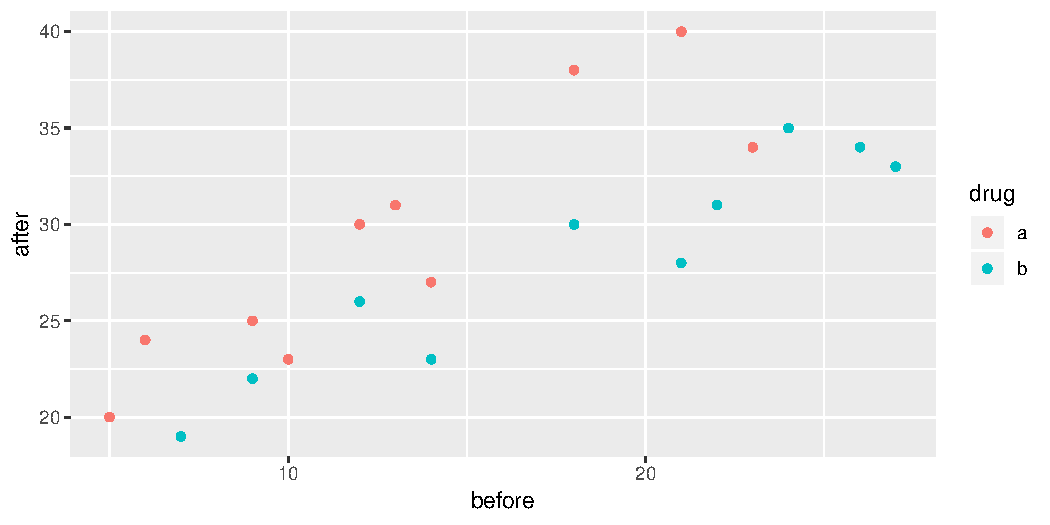
\includegraphics{figure/ancova-plot-1.pdf}
\caption{plot of chunk ancova-plot}
\end{figure}

\end{frame}

\begin{frame}{Comments}
\protect\hypertarget{comments-17}{}

\begin{itemize}
\item
  As before score goes up, after score goes up.
\item
  Red points (drug A) generally above blue points (drug B), for
  comparable before score.
\item
  Suggests before score effect \emph{and} drug effect.
\end{itemize}

\end{frame}

\begin{frame}[fragile]{The means}
\protect\hypertarget{the-means}{}

\begin{Shaded}
\begin{Highlighting}[]
\NormalTok{prepost }\OperatorTok
\StringTok{  }\KeywordTok{group_by}\NormalTok{(drug) }\OperatorTok
\StringTok{  }\KeywordTok{summarize}\NormalTok{(}
    \DataTypeTok{before_mean =} \KeywordTok{mean}\NormalTok{(before),}
    \DataTypeTok{after_mean =} \KeywordTok{mean}\NormalTok{(after)}
\NormalTok{  )}
\end{Highlighting}
\end{Shaded}

\begin{verbatim}
## [conflicted] `summarize` found in 2 packages.
## Either pick the one you want with `::` 
## * plyr::summarize
## * dplyr::summarize
## Or declare a preference with `conflict_prefer()`
## * conflict_prefer("summarize", "plyr")
## * conflict_prefer("summarize", "dplyr")
\end{verbatim}

\begin{itemize}
\item
  Mean ``after'' score slightly higher for treatment A.
\item
  Mean ``before'' score much higher for treatment B.
\item
  Greater \emph{improvement} on treatment A.
\end{itemize}

\end{frame}

\begin{frame}[fragile]{Testing for interaction}
\protect\hypertarget{testing-for-interaction}{}

\begin{Shaded}
\begin{Highlighting}[]
\NormalTok{prepost}\FloatTok{.1}\NormalTok{ <-}\StringTok{ }\KeywordTok{lm}\NormalTok{(after }\OperatorTok{~}\StringTok{ }\NormalTok{before }\OperatorTok{*}\StringTok{ }\NormalTok{drug, }\DataTypeTok{data =}\NormalTok{ prepost)}
\KeywordTok{anova}\NormalTok{(prepost}\FloatTok{.1}\NormalTok{)}
\end{Highlighting}
\end{Shaded}

\begin{verbatim}
## Analysis of Variance Table
## 
## Response: after
##             Df Sum Sq Mean Sq F value    Pr(>F)    
## before       1 430.92  430.92 62.6894  6.34e-07 ***
## drug         1 115.31  115.31 16.7743 0.0008442 ***
## before:drug  1  12.34   12.34  1.7948 0.1990662    
## Residuals   16 109.98    6.87                      
## ---
## Signif. codes:  
## 0 '***' 0.001 '**' 0.01 '*' 0.05 '.' 0.1 ' ' 1
\end{verbatim}

\begin{itemize}
\tightlist
\item
  Interaction not significant. Will remove later.
\end{itemize}

\end{frame}

\begin{frame}[fragile]{Predictions, with interaction included}
\protect\hypertarget{predictions-with-interaction-included}{}

Make combinations of before score and drug:

\begin{Shaded}
\begin{Highlighting}[]
\NormalTok{new <-}\StringTok{ }\KeywordTok{crossing}\NormalTok{(}
  \DataTypeTok{before =} \KeywordTok{c}\NormalTok{(}\DecValTok{5}\NormalTok{, }\DecValTok{15}\NormalTok{, }\DecValTok{25}\NormalTok{),}
  \DataTypeTok{drug =} \KeywordTok{c}\NormalTok{(}\StringTok{"a"}\NormalTok{, }\StringTok{"b"}\NormalTok{)}
\NormalTok{)}
\NormalTok{new}
\end{Highlighting}
\end{Shaded}

\begin{verbatim}
## # A tibble: 6 x 2
##   before drug 
##    <dbl> <chr>
## 1      5 a    
## 2      5 b    
## 3     15 a    
## 4     15 b    
## 5     25 a    
## 6     25 b
\end{verbatim}

\end{frame}

\begin{frame}[fragile]{Do predictions:}
\protect\hypertarget{do-predictions}{}

\begin{Shaded}
\begin{Highlighting}[]
\NormalTok{pred <-}\StringTok{ }\KeywordTok{predict}\NormalTok{(prepost}\FloatTok{.1}\NormalTok{, new)}
\NormalTok{preds <-}\StringTok{ }\KeywordTok{bind_cols}\NormalTok{(new, }\DataTypeTok{pred =}\NormalTok{ pred)}
\NormalTok{preds}
\end{Highlighting}
\end{Shaded}

\begin{verbatim}
## # A tibble: 6 x 3
##   before drug   pred
##    <dbl> <chr> <dbl>
## 1      5 a      21.3
## 2      5 b      18.7
## 3     15 a      31.1
## 4     15 b      25.9
## 5     25 a      40.8
## 6     25 b      33.2
\end{verbatim}

\end{frame}

\begin{frame}[fragile]{Making a plot with lines for each \texttt{drug}}
\protect\hypertarget{making-a-plot-with-lines-for-each-drug}{}

\begin{Shaded}
\begin{Highlighting}[]
\NormalTok{g <-}\StringTok{ }\KeywordTok{ggplot}\NormalTok{(prepost,}
  \KeywordTok{aes}\NormalTok{(}\DataTypeTok{x =}\NormalTok{ before, }\DataTypeTok{y =}\NormalTok{ after, }\DataTypeTok{colour =}\NormalTok{ drug)) }\OperatorTok{+}
\StringTok{  }\KeywordTok{geom_point}\NormalTok{() }\OperatorTok{+}\StringTok{ }\KeywordTok{geom_line}\NormalTok{(}\DataTypeTok{data =}\NormalTok{ preds, }\KeywordTok{aes}\NormalTok{(}\DataTypeTok{y =}\NormalTok{ pred))}
\end{Highlighting}
\end{Shaded}

\begin{itemize}
\item
  Here, final line:

  \begin{itemize}
  \item
    joins points by lines \emph{for different data
    set} (\texttt{preds} rather than \texttt{prepost}),
  \item
    \emph{different \(y\)} (\texttt{pred} rather than \texttt{after}),
  \item
    but same \(x\) (\texttt{x=before} inherited from first
    \texttt{aes}).
  \end{itemize}
\item
  Last line could (more easily) be
\end{itemize}

\begin{Shaded}
\begin{Highlighting}[]
\KeywordTok{geom_smooth}\NormalTok{(}\DataTypeTok{method =} \StringTok{"lm"}\NormalTok{, }\DataTypeTok{se =}\NormalTok{ F)}
\end{Highlighting}
\end{Shaded}

which would work here, but not for later plot.

\end{frame}

\begin{frame}{The plot}
\protect\hypertarget{the-plot-5}{}

\begin{itemize}
\item
  Lines almost parallel, but not quite.
\item
  Non-parallelism (interaction) not significant:
\end{itemize}

\begin{figure}
\centering
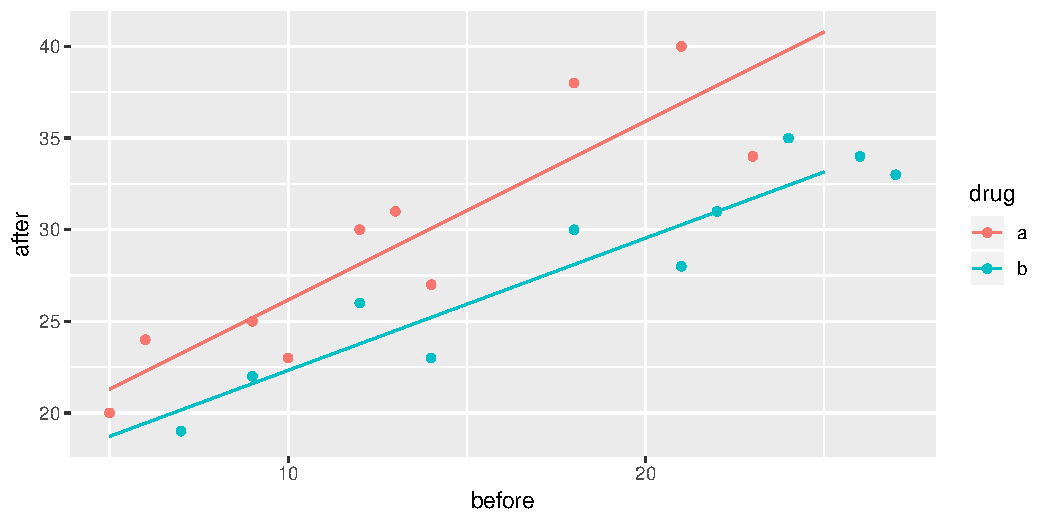
\includegraphics{figure/nachwazzo-1.pdf}
\caption{plot of chunk nachwazzo}
\end{figure}

\end{frame}

\begin{frame}[fragile]{Taking out interaction}
\protect\hypertarget{taking-out-interaction}{}

\small

\begin{Shaded}
\begin{Highlighting}[]
\NormalTok{prepost}\FloatTok{.2}\NormalTok{ <-}\StringTok{ }\KeywordTok{update}\NormalTok{(prepost}\FloatTok{.1}\NormalTok{, . }\OperatorTok{~}\StringTok{ }\NormalTok{. }\OperatorTok{-}\StringTok{ }\NormalTok{before}\OperatorTok{:}\NormalTok{drug)}
\KeywordTok{anova}\NormalTok{(prepost}\FloatTok{.2}\NormalTok{)}
\end{Highlighting}
\end{Shaded}

\begin{verbatim}
## Analysis of Variance Table
## 
## Response: after
##           Df Sum Sq Mean Sq F value    Pr(>F)    
## before     1 430.92  430.92  59.890 5.718e-07 ***
## drug       1 115.31  115.31  16.025 0.0009209 ***
## Residuals 17 122.32    7.20                      
## ---
## Signif. codes:  
## 0 '***' 0.001 '**' 0.01 '*' 0.05 '.' 0.1 ' ' 1
\end{verbatim}

\normalsize

\begin{itemize}
\item
  Take out non-significant interaction.
\item
  \texttt{before} and \texttt{drug} strongly significant.
\item
  Do predictions again and plot them.
\end{itemize}

\end{frame}

\begin{frame}[fragile]{Predicted values again (no-interaction model)}
\protect\hypertarget{predicted-values-again-no-interaction-model}{}

\begin{Shaded}
\begin{Highlighting}[]
\NormalTok{pred <-}\StringTok{ }\KeywordTok{predict}\NormalTok{(prepost}\FloatTok{.2}\NormalTok{, new)}
\NormalTok{preds <-}\StringTok{ }\KeywordTok{bind_cols}\NormalTok{(new, }\DataTypeTok{pred =}\NormalTok{ pred)}
\NormalTok{preds}
\end{Highlighting}
\end{Shaded}

\begin{verbatim}
## # A tibble: 6 x 3
##   before drug   pred
##    <dbl> <chr> <dbl>
## 1      5 a      22.5
## 2      5 b      17.3
## 3     15 a      30.8
## 4     15 b      25.6
## 5     25 a      39.0
## 6     25 b      33.9
\end{verbatim}

Each increase of 10 in before score results in 8.3 in predicted after
score, \emph{the same for both drugs}.

\end{frame}

\begin{frame}[fragile]{Making a plot, again}
\protect\hypertarget{making-a-plot-again}{}

\begin{Shaded}
\begin{Highlighting}[]
\NormalTok{g <-}\StringTok{ }\KeywordTok{ggplot}\NormalTok{(}
\NormalTok{  prepost,}
  \KeywordTok{aes}\NormalTok{(}\DataTypeTok{x =}\NormalTok{ before, }\DataTypeTok{y =}\NormalTok{ after, }\DataTypeTok{colour =}\NormalTok{ drug)}
\NormalTok{) }\OperatorTok{+}
\StringTok{  }\KeywordTok{geom_point}\NormalTok{() }\OperatorTok{+}
\StringTok{  }\KeywordTok{geom_line}\NormalTok{(}\DataTypeTok{data =}\NormalTok{ preds, }\KeywordTok{aes}\NormalTok{(}\DataTypeTok{y =}\NormalTok{ pred))}
\end{Highlighting}
\end{Shaded}

Exactly same as before, but using new predictions.

\end{frame}

\begin{frame}[fragile]{The no-interaction plot of predicted values}
\protect\hypertarget{the-no-interaction-plot-of-predicted-values}{}

\begin{Shaded}
\begin{Highlighting}[]
\NormalTok{g}
\end{Highlighting}
\end{Shaded}

\begin{figure}
\centering
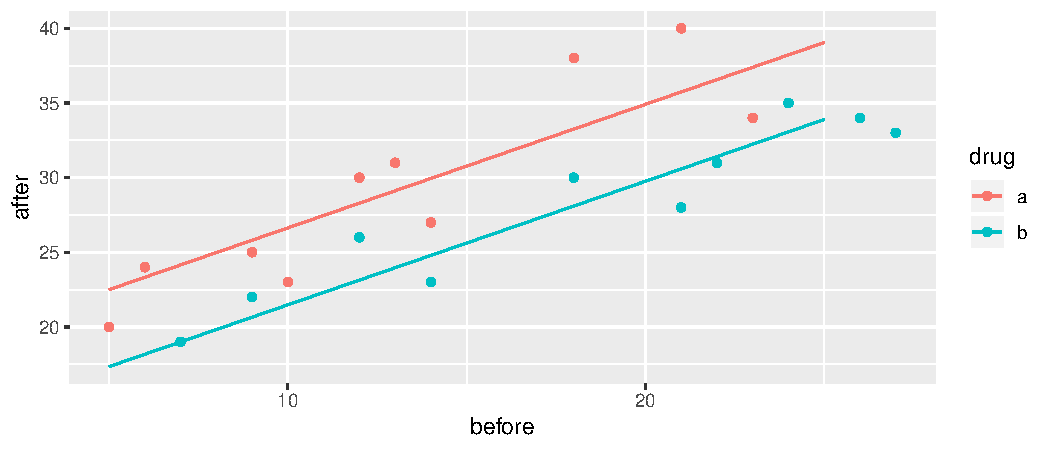
\includegraphics{figure/cabazzo-1.pdf}
\caption{plot of chunk cabazzo}
\end{figure}

Lines now \emph{parallel}. No-interaction model forces them to have the
same slope.

\end{frame}

\begin{frame}[fragile]{Different look at model output}
\protect\hypertarget{different-look-at-model-output}{}

\begin{itemize}
\item
  \texttt{anova(prepost.2)} tests for significant effect of before score
  and of drug, but doesn't help with interpretation.
\item
  \texttt{summary(prepost.2)} views as regression with slopes:
\end{itemize}

\scriptsize

\begin{Shaded}
\begin{Highlighting}[]
\KeywordTok{summary}\NormalTok{(prepost}\FloatTok{.2}\NormalTok{)}
\end{Highlighting}
\end{Shaded}

\begin{verbatim}
## 
## Call:
## lm(formula = after ~ before + drug, data = prepost)
## 
## Residuals:
##     Min      1Q  Median      3Q     Max 
## -3.6348 -2.5099 -0.2038  1.8871  4.7453 
## 
## Coefficients:
##             Estimate Std. Error t value Pr(>|t|)    
## (Intercept)  18.3600     1.5115  12.147 8.35e-10 ***
## before        0.8275     0.0955   8.665 1.21e-07 ***
## drugb        -5.1547     1.2876  -4.003 0.000921 ***
## ---
## Signif. codes:  
## 0 '***' 0.001 '**' 0.01 '*' 0.05 '.' 0.1 ' ' 1
## 
## Residual standard error: 2.682 on 17 degrees of freedom
## Multiple R-squared:  0.817,  Adjusted R-squared:  0.7955 
## F-statistic: 37.96 on 2 and 17 DF,  p-value: 5.372e-07
\end{verbatim}

\normalsize

\end{frame}

\begin{frame}[fragile]{Understanding those slopes}
\protect\hypertarget{understanding-those-slopes}{}

\footnotesize

\begin{Shaded}
\begin{Highlighting}[]
\KeywordTok{tidy}\NormalTok{(prepost}\FloatTok{.2}\NormalTok{)}
\end{Highlighting}
\end{Shaded}

\begin{verbatim}
## # A tibble: 3 x 5
##   term        estimate std.error statistic  p.value
##   <chr>          <dbl>     <dbl>     <dbl>    <dbl>
## 1 (Intercept)   18.4      1.51       12.1  8.35e-10
## 2 before         0.827    0.0955      8.66 1.21e- 7
## 3 drugb         -5.15     1.29       -4.00 9.21e- 4
\end{verbatim}

\normalsize

\begin{itemize}
\item
  \texttt{before} ordinary numerical variable; \texttt{drug}
  categorical.
\item
  \texttt{lm} uses first category \texttt{druga} as baseline.
\item
  Intercept is prediction of after score for before score 0 and
  \emph{drug A}.
\item
  \texttt{before} slope is predicted change in after score when before
  score increases by 1 (usual slope)
\item
  Slope for \texttt{drugb} is \emph{change} in predicted after score for
  being on drug B rather than drug A. Same for \emph{any} before score
  (no interaction).
\end{itemize}

\end{frame}

\begin{frame}{Summary}
\protect\hypertarget{summary}{}

\begin{itemize}
\item
  ANCOVA model: fits different regression line for each group,
  predicting response from covariate.
\item
  ANCOVA model with interaction between factor and covariate allows
  different slopes for each line.
\item
  Sometimes those lines can cross over!
\item
  If interaction not significant, take out. Lines then parallel.
\item
  With parallel lines, groups have consistent effect regardless of value
  of covariate.
\end{itemize}

\end{frame}

\hypertarget{multivariate-anova}{%
\section{Multivariate ANOVA}\label{multivariate-anova}}

\begin{frame}{Multivariate analysis of variance}
\protect\hypertarget{multivariate-analysis-of-variance}{}

\begin{itemize}
\item
  Standard ANOVA has just one response variable.
\item
  What if you have more than one response?
\item
  Try an ANOVA on each response separately.
\item
  But might miss some kinds of interesting dependence between the
  responses that distinguish the groups.
\end{itemize}

\end{frame}

\begin{frame}[fragile]{Packages}
\protect\hypertarget{packages-4}{}

\begin{Shaded}
\begin{Highlighting}[]
\KeywordTok{library}\NormalTok{(car)}
\KeywordTok{library}\NormalTok{(tidyverse)}
\end{Highlighting}
\end{Shaded}

\end{frame}

\begin{frame}[fragile]{Small example}
\protect\hypertarget{small-example}{}

\begin{itemize}
\item
  Measure yield and seed weight of plants grown under 2 conditions: low
  and high amounts of fertilizer.
\item
  Data (fertilizer, yield, seed weight):
\end{itemize}

\begin{Shaded}
\begin{Highlighting}[]
\NormalTok{url <-}\StringTok{ "http://www.utsc.utoronto.ca/~butler/d29/manova1.txt"}
\NormalTok{hilo <-}\StringTok{ }\KeywordTok{read_delim}\NormalTok{(url, }\StringTok{" "}\NormalTok{)}
\end{Highlighting}
\end{Shaded}

\begin{verbatim}
## Parsed with column specification:
## cols(
##   fertilizer = col_character(),
##   yield = col_double(),
##   weight = col_double()
## )
\end{verbatim}

\begin{itemize}
\tightlist
\item
  2 responses, yield and seed weight.
\end{itemize}

\end{frame}

\begin{frame}[fragile]{The data}
\protect\hypertarget{the-data-9}{}

\begin{Shaded}
\begin{Highlighting}[]
\NormalTok{hilo}
\end{Highlighting}
\end{Shaded}

\begin{verbatim}
## # A tibble: 8 x 3
##   fertilizer yield weight
##   <chr>      <dbl>  <dbl>
## 1 low           34     10
## 2 low           29     14
## 3 low           35     11
## 4 low           32     13
## 5 high          33     14
## 6 high          38     12
## 7 high          34     13
## 8 high          35     14
\end{verbatim}

\end{frame}

\begin{frame}[fragile]{Boxplot for yield for each fertilizer group}
\protect\hypertarget{boxplot-for-yield-for-each-fertilizer-group}{}

\begin{Shaded}
\begin{Highlighting}[]
\KeywordTok{ggplot}\NormalTok{(hilo, }\KeywordTok{aes}\NormalTok{(}\DataTypeTok{x =}\NormalTok{ fertilizer, }\DataTypeTok{y =}\NormalTok{ yield)) }\OperatorTok{+}\StringTok{ }\KeywordTok{geom_boxplot}\NormalTok{()}
\end{Highlighting}
\end{Shaded}

\begin{figure}
\centering
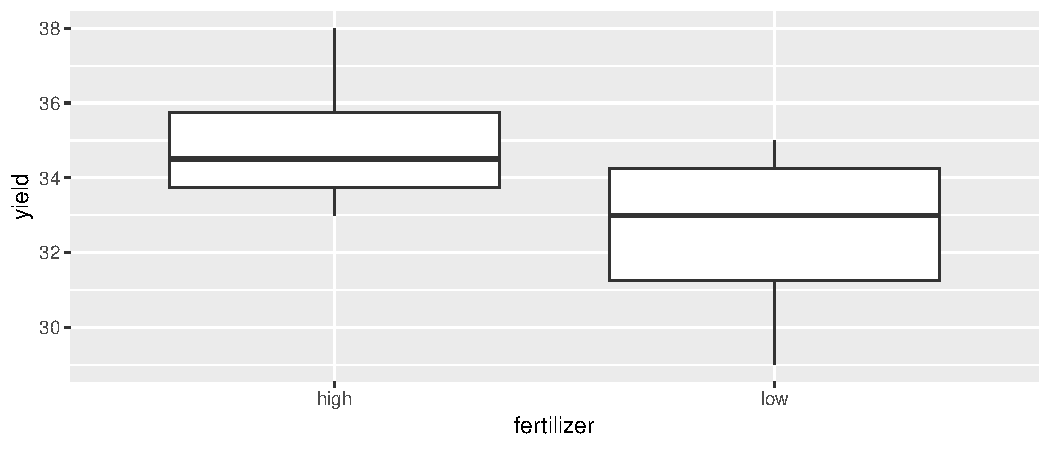
\includegraphics{figure/ferto-1.pdf}
\caption{plot of chunk ferto}
\end{figure}

Yields overlap for fertilizer groups.

\end{frame}

\begin{frame}[fragile]{Boxplot for weight for each fertilizer group}
\protect\hypertarget{boxplot-for-weight-for-each-fertilizer-group}{}

\begin{Shaded}
\begin{Highlighting}[]
\KeywordTok{ggplot}\NormalTok{(hilo, }\KeywordTok{aes}\NormalTok{(}\DataTypeTok{x =}\NormalTok{ fertilizer, }\DataTypeTok{y =}\NormalTok{ weight)) }\OperatorTok{+}\StringTok{ }\KeywordTok{geom_boxplot}\NormalTok{()}
\end{Highlighting}
\end{Shaded}

\begin{figure}
\centering
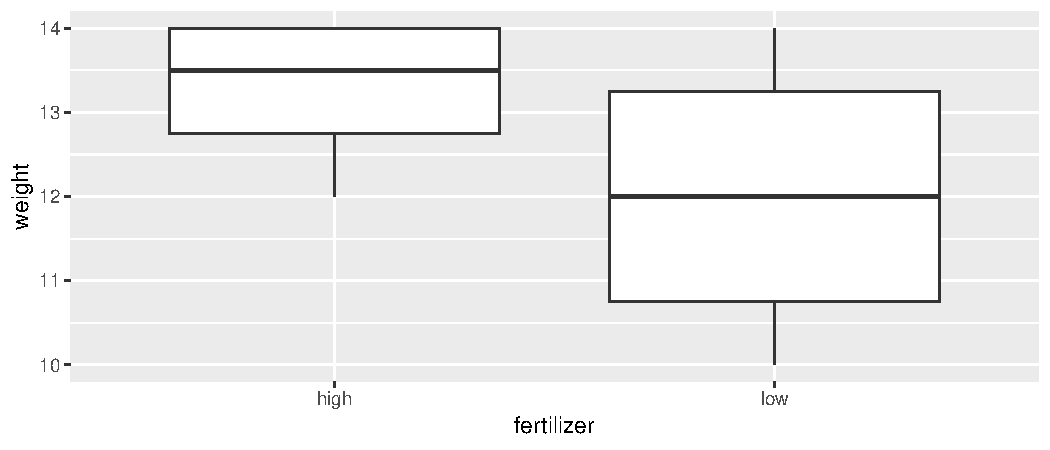
\includegraphics{figure/casteldisangro-1.pdf}
\caption{plot of chunk casteldisangro}
\end{figure}

Weights overlap for fertilizer groups.

\end{frame}

\begin{frame}[fragile]{ANOVAs for yield and weight}
\protect\hypertarget{anovas-for-yield-and-weight}{}

\small

\begin{Shaded}
\begin{Highlighting}[]
\NormalTok{hilo.y <-}\StringTok{ }\KeywordTok{aov}\NormalTok{(yield }\OperatorTok{~}\StringTok{ }\NormalTok{fertilizer, }\DataTypeTok{data =}\NormalTok{ hilo)}
\KeywordTok{summary}\NormalTok{(hilo.y)}
\end{Highlighting}
\end{Shaded}

\begin{verbatim}
##             Df Sum Sq Mean Sq F value Pr(>F)
## fertilizer   1   12.5  12.500   2.143  0.194
## Residuals    6   35.0   5.833
\end{verbatim}

\begin{Shaded}
\begin{Highlighting}[]
\NormalTok{hilo.w <-}\StringTok{ }\KeywordTok{aov}\NormalTok{(weight }\OperatorTok{~}\StringTok{ }\NormalTok{fertilizer, }\DataTypeTok{data =}\NormalTok{ hilo)}
\KeywordTok{summary}\NormalTok{(hilo.w)}
\end{Highlighting}
\end{Shaded}

\begin{verbatim}
##             Df Sum Sq Mean Sq F value Pr(>F)
## fertilizer   1  3.125   3.125   1.471  0.271
## Residuals    6 12.750   2.125
\end{verbatim}

\normalsize

Neither response depends significantly on fertilizer. But\ldots

\end{frame}

\begin{frame}[fragile]{Plotting both responses at once}
\protect\hypertarget{plotting-both-responses-at-once}{}

\begin{itemize}
\item
  Have two response variables (not more), so can plot the response
  variables against \emph{each other}, labelling points by which
  fertilizer group they're from.
\item
  First, create data frame with points \((31,14)\) and \((38,10)\) (why?
  Later):
\end{itemize}

\begin{Shaded}
\begin{Highlighting}[]
\NormalTok{d <-}\StringTok{ }\KeywordTok{tribble}\NormalTok{(}
  \OperatorTok{~}\NormalTok{line_x, }\OperatorTok{~}\NormalTok{line_y,}
  \DecValTok{31}\NormalTok{, }\DecValTok{14}\NormalTok{,}
  \DecValTok{38}\NormalTok{, }\DecValTok{10}
\NormalTok{)}
\end{Highlighting}
\end{Shaded}

\begin{itemize}
\tightlist
\item
  Then plot data as points, and add line through points in \texttt{d}:
\end{itemize}

\begin{Shaded}
\begin{Highlighting}[]
\NormalTok{g <-}\StringTok{ }\KeywordTok{ggplot}\NormalTok{(hilo, }\KeywordTok{aes}\NormalTok{(}\DataTypeTok{x =}\NormalTok{ yield, }\DataTypeTok{y =}\NormalTok{ weight,}
                      \DataTypeTok{colour =}\NormalTok{ fertilizer)) }\OperatorTok{+}\StringTok{ }\KeywordTok{geom_point}\NormalTok{() }\OperatorTok{+}
\StringTok{  }\KeywordTok{geom_line}\NormalTok{(}\DataTypeTok{data =}\NormalTok{ d,}
            \KeywordTok{aes}\NormalTok{(}\DataTypeTok{x =}\NormalTok{ line_x, }\DataTypeTok{y =}\NormalTok{ line_y, }\DataTypeTok{colour =} \OtherTok{NULL}\NormalTok{))}
\end{Highlighting}
\end{Shaded}

\end{frame}

\begin{frame}{The plot}
\protect\hypertarget{the-plot-6}{}

\begin{figure}
\centering
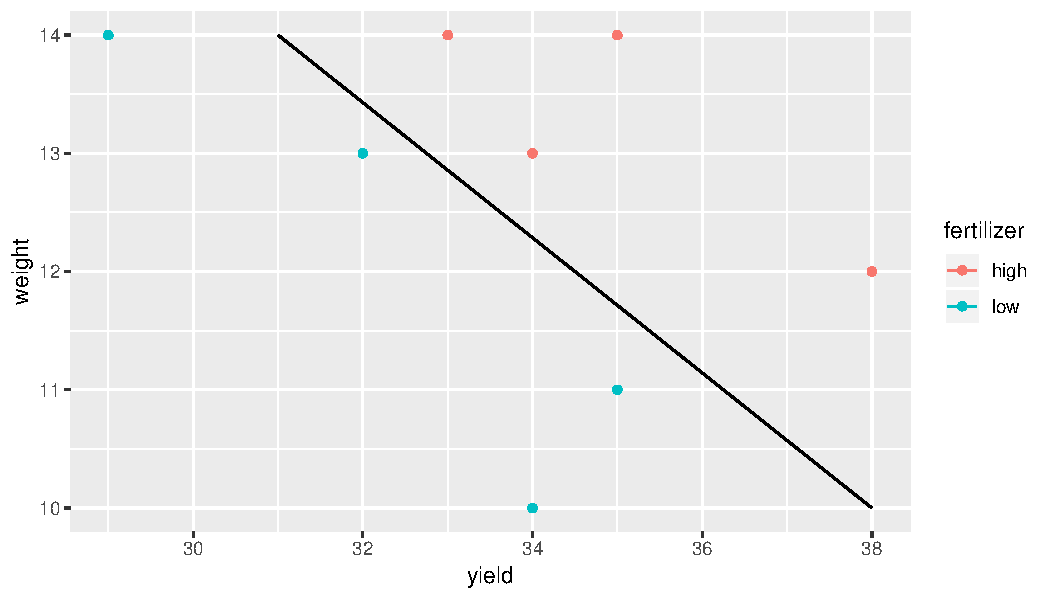
\includegraphics{figure/charlecombe-1.pdf}
\caption{plot of chunk charlecombe}
\end{figure}

\end{frame}

\begin{frame}[fragile]{Comments}
\protect\hypertarget{comments-18}{}

\begin{itemize}
\tightlist
\item
  Graph construction:

  \begin{itemize}
  \tightlist
  \item
    Joining points in \texttt{d} by line.
  \item
    \texttt{geom\_line} inherits \texttt{colour} from \texttt{aes} in
    \texttt{ggplot}.
  \item
    Data frame \texttt{d} has no \texttt{fertilizer} (previous
    \texttt{colour}), so have to unset.
  \end{itemize}
\item
  Results:

  \begin{itemize}
  \item
    High-fertilizer plants have both yield and weight high.
  \item
    True even though no sig difference in yield or weight individually.
  \item
    Drew line separating highs from lows on plot.
  \end{itemize}
\end{itemize}

\end{frame}

\begin{frame}[fragile]{MANOVA finds multivariate differences}
\protect\hypertarget{manova-finds-multivariate-differences}{}

\begin{itemize}
\tightlist
\item
  Is difference found by diagonal line significant? MANOVA finds out.
\end{itemize}

\begin{Shaded}
\begin{Highlighting}[]
\NormalTok{response <-}\StringTok{ }\KeywordTok{with}\NormalTok{(hilo, }\KeywordTok{cbind}\NormalTok{(yield, weight))}
\NormalTok{hilo}\FloatTok{.1}\NormalTok{ <-}\StringTok{ }\KeywordTok{manova}\NormalTok{(response }\OperatorTok{~}\StringTok{ }\NormalTok{fertilizer, }\DataTypeTok{data =}\NormalTok{ hilo)}
\KeywordTok{summary}\NormalTok{(hilo}\FloatTok{.1}\NormalTok{)}
\end{Highlighting}
\end{Shaded}

\begin{verbatim}
##            Df  Pillai approx F num Df den Df  Pr(>F)  
## fertilizer  1 0.80154   10.097      2      5 0.01755 *
## Residuals   6                                         
## ---
## Signif. codes:  
## 0 '***' 0.001 '**' 0.01 '*' 0.05 '.' 0.1 ' ' 1
\end{verbatim}

\begin{itemize}
\tightlist
\item
  Yes! Difference between groups is \emph{diagonally}, not just up/down
  (weight) or left-right (yield). The \emph{yield-weight combination}
  matters.
\end{itemize}

\end{frame}

\begin{frame}[fragile]{Strategy}
\protect\hypertarget{strategy}{}

\begin{itemize}
\item
  Create new response variable by gluing together columns of responses,
  using \texttt{cbind}.
\item
  Use \texttt{manova} with new response, looks like \texttt{lm}
  otherwise.
\item
  With more than 2 responses, cannot draw graph. What then?
\item
  If MANOVA test significant, cannot use Tukey. What then?
\item
  Use \emph{discriminant analysis} (of which more later).
\end{itemize}

\end{frame}

\begin{frame}[fragile]{Another way to do MANOVA}
\protect\hypertarget{another-way-to-do-manova}{}

Install (once) and load package \texttt{car}:

\begin{Shaded}
\begin{Highlighting}[]
\KeywordTok{library}\NormalTok{(car)}
\end{Highlighting}
\end{Shaded}

\end{frame}

\begin{frame}[fragile]{Another way\ldots}
\protect\hypertarget{another-way-1}{}

\begin{Shaded}
\begin{Highlighting}[]
\NormalTok{hilo.}\FloatTok{2.}\NormalTok{lm <-}\StringTok{ }\KeywordTok{lm}\NormalTok{(response }\OperatorTok{~}\StringTok{ }\NormalTok{fertilizer, }\DataTypeTok{data =}\NormalTok{ hilo)}
\NormalTok{hilo}\FloatTok{.2}\NormalTok{ <-}\StringTok{ }\KeywordTok{Manova}\NormalTok{(hilo.}\FloatTok{2.}\NormalTok{lm)}
\NormalTok{hilo}\FloatTok{.2}
\end{Highlighting}
\end{Shaded}

\begin{verbatim}
## 
## Type II MANOVA Tests: Pillai test statistic
##            Df test stat approx F num Df den Df  Pr(>F)  
## fertilizer  1   0.80154   10.097      2      5 0.01755 *
## ---
## Signif. codes:  
## 0 '***' 0.001 '**' 0.01 '*' 0.05 '.' 0.1 ' ' 1
\end{verbatim}

\begin{itemize}
\item
  Same result as small-m \texttt{manova}.
\item
  \texttt{Manova} will also do \emph{repeated measures}, coming up
  later.
\end{itemize}

\end{frame}

\begin{frame}[fragile]{Another example: peanuts}
\protect\hypertarget{another-example-peanuts}{}

\begin{itemize}
\item
  Three different varieties of peanuts (mysteriously, 5, 6 and 8)
  planted in two different locations.
\item
  Three response variables: \texttt{y}, \texttt{smk} and \texttt{w}.
\end{itemize}

\begin{Shaded}
\begin{Highlighting}[]
\NormalTok{u <-}\StringTok{ "http://www.utsc.utoronto.ca/~butler/d29/peanuts.txt"}
\NormalTok{peanuts.orig <-}\StringTok{ }\KeywordTok{read_delim}\NormalTok{(u, }\StringTok{" "}\NormalTok{)}
\end{Highlighting}
\end{Shaded}

\begin{verbatim}
## Parsed with column specification:
## cols(
##   obs = col_double(),
##   location = col_double(),
##   variety = col_double(),
##   y = col_double(),
##   smk = col_double(),
##   w = col_double()
## )
\end{verbatim}

\end{frame}

\begin{frame}[fragile]{The data}
\protect\hypertarget{the-data-10}{}

\small

\begin{Shaded}
\begin{Highlighting}[]
\NormalTok{peanuts.orig}
\end{Highlighting}
\end{Shaded}

\begin{verbatim}
## # A tibble: 12 x 6
##      obs location variety     y   smk     w
##    <dbl>    <dbl>   <dbl> <dbl> <dbl> <dbl>
##  1     1        1       5  195.  153.  51.4
##  2     2        1       5  194.  168.  53.7
##  3     3        2       5  190.  140.  55.5
##  4     4        2       5  180.  121.  44.4
##  5     5        1       6  203   157.  49.8
##  6     6        1       6  196.  166   45.8
##  7     7        2       6  203.  166.  60.4
##  8     8        2       6  198.  162.  54.1
##  9     9        1       8  194.  164.  57.8
## 10    10        1       8  187   165.  58.6
## 11    11        2       8  202.  167.  65  
## 12    12        2       8  200   174.  67.2
\end{verbatim}

\normalsize

\end{frame}

\begin{frame}[fragile]{Setup for analysis}
\protect\hypertarget{setup-for-analysis}{}

\begin{Shaded}
\begin{Highlighting}[]
\NormalTok{peanuts <-}\StringTok{ }\NormalTok{peanuts.orig }\OperatorTok
\StringTok{  }\KeywordTok{mutate}\NormalTok{(}
    \DataTypeTok{location =} \KeywordTok{factor}\NormalTok{(location),}
    \DataTypeTok{variety =} \KeywordTok{factor}\NormalTok{(variety)}
\NormalTok{  )}
\NormalTok{response <-}\StringTok{ }\KeywordTok{with}\NormalTok{(peanuts, }\KeywordTok{cbind}\NormalTok{(y, smk, w))}
\KeywordTok{head}\NormalTok{(response)}
\end{Highlighting}
\end{Shaded}

\begin{verbatim}
##          y   smk    w
## [1,] 195.3 153.1 51.4
## [2,] 194.3 167.7 53.7
## [3,] 189.7 139.5 55.5
## [4,] 180.4 121.1 44.4
## [5,] 203.0 156.8 49.8
## [6,] 195.9 166.0 45.8
\end{verbatim}

\end{frame}

\begin{frame}[fragile]{Analysis (using \texttt{Manova)}}
\protect\hypertarget{analysis-using-manova}{}

\small

\begin{Shaded}
\begin{Highlighting}[]
\NormalTok{peanuts}\FloatTok{.1}\NormalTok{ <-}\StringTok{ }\KeywordTok{lm}\NormalTok{(response }\OperatorTok{~}\StringTok{ }\NormalTok{location }\OperatorTok{*}\StringTok{ }\NormalTok{variety, }\DataTypeTok{data =}\NormalTok{ peanuts)}
\NormalTok{peanuts}\FloatTok{.2}\NormalTok{ <-}\StringTok{ }\KeywordTok{Manova}\NormalTok{(peanuts}\FloatTok{.1}\NormalTok{)}
\NormalTok{peanuts}\FloatTok{.2}
\end{Highlighting}
\end{Shaded}

\begin{verbatim}
## 
## Type II MANOVA Tests: Pillai test statistic
##                  Df test stat approx F num Df den Df
## location          1   0.89348  11.1843      3      4
## variety           2   1.70911   9.7924      6     10
## location:variety  2   1.29086   3.0339      6     10
##                    Pr(>F)   
## location         0.020502 * 
## variety          0.001056 **
## location:variety 0.058708 . 
## ---
## Signif. codes:  
## 0 '***' 0.001 '**' 0.01 '*' 0.05 '.' 0.1 ' ' 1
\end{verbatim}

\normalsize

\end{frame}

\begin{frame}[fragile]{Comments}
\protect\hypertarget{comments-19}{}

\begin{itemize}
\item
  Interaction not quite significant, but main effects are.
\item
  Combined response variable \texttt{(y,smk,w)} definitely depends on
  location and on variety
\item
  Weak dependence of \texttt{(y,smk,w)} on the location-variety
  \emph{combination.}
\item
  Understanding that dependence beyond our scope right now.
\end{itemize}

\end{frame}

\hypertarget{repeated-measures-by-profile-analysis}{%
\section{Repeated measures by profile
analysis}\label{repeated-measures-by-profile-analysis}}

\begin{frame}[fragile]{Repeated measures by profile analysis}
\protect\hypertarget{repeated-measures-by-profile-analysis-1}{}

\begin{itemize}
\item
  More than one response \emph{measurement} for each subject. Might be
\item
  measurements of the same thing at different times
\item
  measurements of different but related things
\item
  Generalization of matched pairs (``matched triples'', etc.).
\item
  Variation: each subject does several different treatments at different
  times (called \emph{crossover design}).
\item
  Expect measurements on same subject to be correlated, so assumptions
  of independence will fail.
\item
  Called \emph{repeated measures}. Different approaches, but
  \emph{profile analysis} uses \texttt{Manova} (set up right way).
\item
  Another approach uses \emph{mixed models} (random effects).
\end{itemize}

\end{frame}

\begin{frame}[fragile]{Packages}
\protect\hypertarget{packages-5}{}

\begin{Shaded}
\begin{Highlighting}[]
\KeywordTok{library}\NormalTok{(car)}
\KeywordTok{library}\NormalTok{(tidyverse)}
\end{Highlighting}
\end{Shaded}

\end{frame}

\begin{frame}[fragile]{Example: histamine in dogs}
\protect\hypertarget{example-histamine-in-dogs}{}

\begin{itemize}
\item
  8 dogs take part in experiment.
\item
  Dogs randomized to one of 2 different drugs.
\item
  Response: log of blood concentration of histamine 0, 1, 3 and 5
  minutes after taking drug. (Repeated measures.)
\item
  Data in \texttt{dogs.txt}, column-aligned.
\end{itemize}

\end{frame}

\begin{frame}[fragile]{Read in data}
\protect\hypertarget{read-in-data-3}{}

\begin{Shaded}
\begin{Highlighting}[]
\NormalTok{my_url <-}\StringTok{ "http://www.utsc.utoronto.ca/~butler/d29/dogs.txt"}
\NormalTok{dogs <-}\StringTok{ }\KeywordTok{read_table}\NormalTok{(my_url)}
\end{Highlighting}
\end{Shaded}

\begin{verbatim}
## Parsed with column specification:
## cols(
##   dog = col_character(),
##   drug = col_character(),
##   x = col_character(),
##   lh0 = col_double(),
##   lh1 = col_double(),
##   lh3 = col_double(),
##   lh5 = col_double()
## )
\end{verbatim}

\end{frame}

\begin{frame}[fragile]{Setting things up}
\protect\hypertarget{setting-things-up}{}

\begin{Shaded}
\begin{Highlighting}[]
\NormalTok{dogs}
\end{Highlighting}
\end{Shaded}

\begin{verbatim}
## # A tibble: 8 x 7
##   dog   drug         x       lh0   lh1   lh3   lh5
##   <chr> <chr>        <chr> <dbl> <dbl> <dbl> <dbl>
## 1 A     Morphine     N     -3.22 -1.61 -2.3  -2.53
## 2 B     Morphine     N     -3.91 -2.81 -3.91 -3.91
## 3 C     Morphine     N     -2.66  0.34 -0.73 -1.43
## 4 D     Morphine     N     -1.77 -0.56 -1.05 -1.43
## 5 E     Trimethaphan N     -3.51 -0.48 -1.17 -1.51
## 6 F     Trimethaphan N     -3.51  0.05 -0.31 -0.51
## 7 G     Trimethaphan N     -2.66 -0.19  0.07 -0.22
## 8 H     Trimethaphan N     -2.41  1.14  0.72  0.21
\end{verbatim}

\begin{Shaded}
\begin{Highlighting}[]
\NormalTok{response <-}\StringTok{ }\KeywordTok{with}\NormalTok{(dogs, }\KeywordTok{cbind}\NormalTok{(lh0, lh1, lh3, lh5))}
\NormalTok{dogs}\FloatTok{.1}\NormalTok{ <-}\StringTok{ }\KeywordTok{lm}\NormalTok{(response }\OperatorTok{~}\StringTok{ }\NormalTok{drug, }\DataTypeTok{data =}\NormalTok{ dogs)}
\end{Highlighting}
\end{Shaded}

\end{frame}

\begin{frame}[fragile]{The repeated measures MANOVA}
\protect\hypertarget{the-repeated-measures-manova}{}

Get list of response variable names; we call them \texttt{times}. Save
in data frame.

\footnotesize

\begin{Shaded}
\begin{Highlighting}[]
\NormalTok{times <-}\StringTok{ }\KeywordTok{colnames}\NormalTok{(response)}
\NormalTok{times.df <-}\StringTok{ }\KeywordTok{data.frame}\NormalTok{(times)}
\NormalTok{dogs}\FloatTok{.2}\NormalTok{ <-}\StringTok{ }\KeywordTok{Manova}\NormalTok{(dogs}\FloatTok{.1}\NormalTok{,}
  \DataTypeTok{idata =}\NormalTok{ times.df,}
  \DataTypeTok{idesign =} \OperatorTok{~}\NormalTok{times}
\NormalTok{)}
\NormalTok{dogs}\FloatTok{.2}
\end{Highlighting}
\end{Shaded}

\begin{verbatim}
## 
## Type II Repeated Measures MANOVA Tests: Pillai test statistic
##             Df test stat approx F num Df den Df   Pr(>F)   
## (Intercept)  1   0.76347  19.3664      1      6 0.004565 **
## drug         1   0.34263   3.1272      1      6 0.127406   
## times        1   0.94988  25.2690      3      4 0.004631 **
## drug:times   1   0.89476  11.3362      3      4 0.020023 * 
## ---
## Signif. codes:  
## 0 '***' 0.001 '**' 0.01 '*' 0.05 '.' 0.1 ' ' 1
\end{verbatim}

\normalsize

\end{frame}

\begin{frame}{Wide and long format}
\protect\hypertarget{wide-and-long-format}{}

\begin{itemize}
\item
  Interaction significant. Pattern of response over time different for
  the two drugs.
\item
  Want to investigate interaction.
\end{itemize}

\end{frame}

\begin{frame}[fragile]{The wrong shape}
\protect\hypertarget{the-wrong-shape}{}

\begin{itemize}
\tightlist
\item
  But data frame has several observations per line (``wide format''):
\end{itemize}

\scriptsize

\begin{Shaded}
\begin{Highlighting}[]
\NormalTok{dogs }\OperatorTok\StringTok{ }\KeywordTok{slice}\NormalTok{(}\DecValTok{1}\OperatorTok{:}\DecValTok{6}\NormalTok{)}
\end{Highlighting}
\end{Shaded}

\begin{verbatim}
## # A tibble: 6 x 7
##   dog   drug         x       lh0   lh1   lh3   lh5
##   <chr> <chr>        <chr> <dbl> <dbl> <dbl> <dbl>
## 1 A     Morphine     N     -3.22 -1.61 -2.3  -2.53
## 2 B     Morphine     N     -3.91 -2.81 -3.91 -3.91
## 3 C     Morphine     N     -2.66  0.34 -0.73 -1.43
## 4 D     Morphine     N     -1.77 -0.56 -1.05 -1.43
## 5 E     Trimethaphan N     -3.51 -0.48 -1.17 -1.51
## 6 F     Trimethaphan N     -3.51  0.05 -0.31 -0.51
\end{verbatim}

\normalsize

\begin{itemize}
\item
  Plotting works with data in ``long format'': one response per line.
\item
  The responses are log-histamine at different times, labelled
  \texttt{lh}-something. Call them all \texttt{lh} and put them in one
  column, with the time they belong to labelled.
\end{itemize}

\end{frame}

\begin{frame}[fragile]{Running \texttt{gather}, try 1}
\protect\hypertarget{running-gather-try-1}{}

\footnotesize

\begin{Shaded}
\begin{Highlighting}[]
\NormalTok{dogs }\OperatorTok\StringTok{ }\KeywordTok{gather}\NormalTok{(time, lh, lh0}\OperatorTok{:}\NormalTok{lh5) }
\end{Highlighting}
\end{Shaded}

\begin{verbatim}
## # A tibble: 32 x 5
##    dog   drug         x     time     lh
##    <chr> <chr>        <chr> <chr> <dbl>
##  1 A     Morphine     N     lh0   -3.22
##  2 B     Morphine     N     lh0   -3.91
##  3 C     Morphine     N     lh0   -2.66
##  4 D     Morphine     N     lh0   -1.77
##  5 E     Trimethaphan N     lh0   -3.51
##  6 F     Trimethaphan N     lh0   -3.51
##  7 G     Trimethaphan N     lh0   -2.66
##  8 H     Trimethaphan N     lh0   -2.41
##  9 A     Morphine     N     lh1   -1.61
## 10 B     Morphine     N     lh1   -2.81
## # … with 22 more rows
\end{verbatim}

\normalsize

\end{frame}

\begin{frame}[fragile]{Getting the times}
\protect\hypertarget{getting-the-times}{}

Not quite right: for the times, we want just the numbers, not the
letters \texttt{lh} every time. Want new variable containing just number
in \texttt{time}: \texttt{parse\_number}.

\footnotesize

\begin{Shaded}
\begin{Highlighting}[]
\NormalTok{dogs }\OperatorTok
\StringTok{  }\KeywordTok{gather}\NormalTok{(timex, lh, lh0}\OperatorTok{:}\NormalTok{lh5) }\OperatorTok
\StringTok{  }\KeywordTok{mutate}\NormalTok{(}\DataTypeTok{time =} \KeywordTok{parse_number}\NormalTok{(timex)) }
\end{Highlighting}
\end{Shaded}

\begin{verbatim}
## # A tibble: 32 x 6
##    dog   drug         x     timex    lh  time
##    <chr> <chr>        <chr> <chr> <dbl> <dbl>
##  1 A     Morphine     N     lh0   -3.22     0
##  2 B     Morphine     N     lh0   -3.91     0
##  3 C     Morphine     N     lh0   -2.66     0
##  4 D     Morphine     N     lh0   -1.77     0
##  5 E     Trimethaphan N     lh0   -3.51     0
##  6 F     Trimethaphan N     lh0   -3.51     0
##  7 G     Trimethaphan N     lh0   -2.66     0
##  8 H     Trimethaphan N     lh0   -2.41     0
##  9 A     Morphine     N     lh1   -1.61     1
## 10 B     Morphine     N     lh1   -2.81     1
## # … with 22 more rows
\end{verbatim}

\normalsize

\end{frame}

\begin{frame}[fragile]{What I did differently}
\protect\hypertarget{what-i-did-differently}{}

\begin{itemize}
\item
  I realized that \texttt{gather} was going to produce something like
  \texttt{lh1}, which I needed to do something further with, so this
  time I gave it a temporary name \texttt{timex}.
\item
  This enabled me to use the name \texttt{time} for the actual numeric
  time.
\item
  This works now, so next save into a new data frame \texttt{dogs.long}.
\end{itemize}

\end{frame}

\begin{frame}[fragile]{Saving the pipelined results}
\protect\hypertarget{saving-the-pipelined-results}{}

\begin{Shaded}
\begin{Highlighting}[]
\NormalTok{dogs }\OperatorTok
\StringTok{  }\KeywordTok{gather}\NormalTok{(timex, lh, lh0}\OperatorTok{:}\NormalTok{lh5) }\OperatorTok
\StringTok{  }\KeywordTok{mutate}\NormalTok{(}\DataTypeTok{time =} \KeywordTok{parse_number}\NormalTok{(timex)) ->}\StringTok{ }\NormalTok{dogs.long}
\end{Highlighting}
\end{Shaded}

This says:

\begin{itemize}
\item
  Take data frame dogs, and then:
\item
  Combine the columns \texttt{lh0} through \texttt{lh5} into one column
  called \texttt{lh}, with the column that each \texttt{lh} value
  originally came from labelled by \texttt{timex}, and then:
\item
  Pull out numeric values in \texttt{timex}, saving in \texttt{time} and
  then:
\item
  save the result in a data frame \texttt{dogs.long}.
\end{itemize}

\end{frame}

\begin{frame}[fragile]{Interaction plot}
\protect\hypertarget{interaction-plot-3}{}

\small

\begin{Shaded}
\begin{Highlighting}[]
\KeywordTok{ggplot}\NormalTok{(dogs.long, }\KeywordTok{aes}\NormalTok{(}\DataTypeTok{x =}\NormalTok{ time, }\DataTypeTok{y =}\NormalTok{ lh, }
                      \DataTypeTok{colour =}\NormalTok{ drug, }\DataTypeTok{group =}\NormalTok{ drug)) }\OperatorTok{+}
\StringTok{  }\KeywordTok{stat_summary}\NormalTok{(}\DataTypeTok{fun.y =}\NormalTok{ mean, }\DataTypeTok{geom =} \StringTok{"point"}\NormalTok{) }\OperatorTok{+}
\StringTok{  }\KeywordTok{stat_summary}\NormalTok{(}\DataTypeTok{fun.y =}\NormalTok{ mean, }\DataTypeTok{geom =} \StringTok{"line"}\NormalTok{)}
\end{Highlighting}
\end{Shaded}

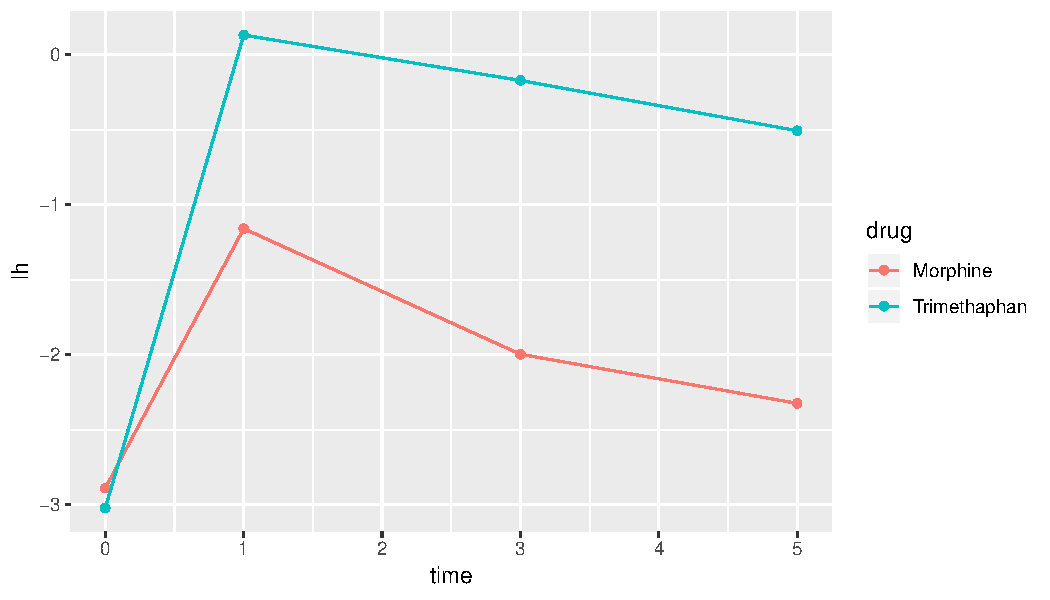
\includegraphics{figure/unnamed-chunk-250-1.pdf} \normalsize

\end{frame}

\begin{frame}[fragile]{Comments}
\protect\hypertarget{comments-20}{}

\begin{itemize}
\item
  Plot mean \texttt{lh} value at each time, joining points on same drug
  by lines.
\item
  drugs same at time 0
\item
  after that, Trimethaphan higher than Morphine.
\item
  Effect of drug not consistent over time: significant interaction.
\end{itemize}

\end{frame}

\begin{frame}[fragile]{Take out time zero}
\protect\hypertarget{take-out-time-zero}{}

\begin{itemize}
\item
  Lines on interaction plot would then be parallel, and so interaction
  should no longer be significant.
\item
  Go back to original ``wide'' \texttt{dogs} data frame.
\end{itemize}

\begin{Shaded}
\begin{Highlighting}[]
\NormalTok{response <-}\StringTok{ }\KeywordTok{with}\NormalTok{(dogs, }\KeywordTok{cbind}\NormalTok{(lh1, lh3, lh5)) }\CommentTok{# excl time 0}
\NormalTok{dogs}\FloatTok{.1}\NormalTok{ <-}\StringTok{ }\KeywordTok{lm}\NormalTok{(response }\OperatorTok{~}\StringTok{ }\NormalTok{drug, }\DataTypeTok{data =}\NormalTok{ dogs)}
\NormalTok{times <-}\StringTok{ }\KeywordTok{colnames}\NormalTok{(response)}
\NormalTok{times.df <-}\StringTok{ }\KeywordTok{data.frame}\NormalTok{(times)}
\NormalTok{dogs}\FloatTok{.2}\NormalTok{ <-}\StringTok{ }\KeywordTok{Manova}\NormalTok{(dogs}\FloatTok{.1}\NormalTok{,}
  \DataTypeTok{idata =}\NormalTok{ times.df,}
  \DataTypeTok{idesign =} \OperatorTok{~}\NormalTok{times}
\NormalTok{)}
\end{Highlighting}
\end{Shaded}

\end{frame}

\begin{frame}[fragile]{Results and comments}
\protect\hypertarget{results-and-comments}{}

\footnotesize

\begin{Shaded}
\begin{Highlighting}[]
\NormalTok{dogs}\FloatTok{.2}
\end{Highlighting}
\end{Shaded}

\begin{verbatim}
## 
## Type II Repeated Measures MANOVA Tests: Pillai test statistic
##             Df test stat approx F num Df den Df   Pr(>F)   
## (Intercept)  1   0.54582   7.2106      1      6 0.036281 * 
## drug         1   0.44551   4.8207      1      6 0.070527 . 
## times        1   0.85429  14.6569      2      5 0.008105 **
## drug:times   1   0.43553   1.9289      2      5 0.239390   
## ---
## Signif. codes:  
## 0 '***' 0.001 '**' 0.01 '*' 0.05 '.' 0.1 ' ' 1
\end{verbatim}

\normalsize

\begin{itemize}
\item
  Correct: interaction no longer significant.
\item
  Significant effect of time.
\item
  Drug effect not quite significant (some variety among dogs within
  drug).
\end{itemize}

\end{frame}

\begin{frame}[fragile]{Is the non-significant drug effect reasonable?}
\protect\hypertarget{is-the-non-significant-drug-effect-reasonable}{}

\begin{itemize}
\item
  Plot \emph{actual data}: \texttt{lh} against \texttt{days}, labelling
  observations by drug: ``spaghetti plot''.
\item
  Uses long data frame (confusing, yes I know):
\item
  Plot (time,lh) points coloured by drug
\item
  and connecting measurements for each \emph{dog} by lines.
\item
  This time, we want \texttt{group=dog} (want the measurements for each
  \emph{dog} joined by lines), but \texttt{colour=drug}:
\end{itemize}

\begin{Shaded}
\begin{Highlighting}[]
\NormalTok{g <-}\StringTok{ }\KeywordTok{ggplot}\NormalTok{(dogs.long, }\KeywordTok{aes}\NormalTok{(}
  \DataTypeTok{x =}\NormalTok{ time, }\DataTypeTok{y =}\NormalTok{ lh,}
  \DataTypeTok{colour =}\NormalTok{ drug, }\DataTypeTok{group =}\NormalTok{ dog}
\NormalTok{)) }\OperatorTok{+}
\StringTok{  }\KeywordTok{geom_point}\NormalTok{() }\OperatorTok{+}\StringTok{ }\KeywordTok{geom_line}\NormalTok{()}
\end{Highlighting}
\end{Shaded}

\end{frame}

\begin{frame}[fragile]{The spaghetti plot}
\protect\hypertarget{the-spaghetti-plot}{}

\begin{Shaded}
\begin{Highlighting}[]
\NormalTok{g}
\end{Highlighting}
\end{Shaded}

\begin{figure}
\centering
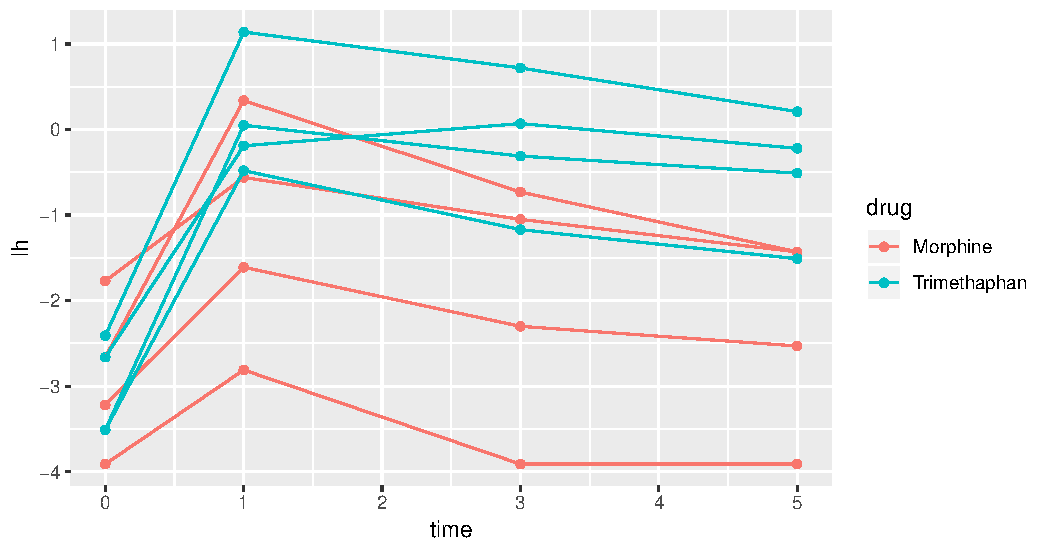
\includegraphics{figure/hoverla-1.pdf}
\caption{plot of chunk hoverla}
\end{figure}

\end{frame}

\begin{frame}[fragile]{Comments}
\protect\hypertarget{comments-21}{}

\begin{itemize}
\item
  For each dog over time, there is a strong increase and gradual
  decrease in log-histamine. This explains the significant time effect.
\item
  The pattern is more or less the same for each dog, regardless of drug.
  This explains the non-significant interaction.
\item
  Most of the trimethaphan dogs (blue) have higher log-histamine
  throughout (time 1 and after), and some of the morphine dogs have
  lower.
\item
  \emph{But} two of the morphine dogs have log-histamine profiles like
  the trimethaphan dogs. This ambiguity is probably why the
  \texttt{drug} effect is not quite significant.
\end{itemize}

\end{frame}

\begin{frame}{The exercise data}
\protect\hypertarget{the-exercise-data}{}

\begin{itemize}
\item
  30 people took part in an exercise study.
\item
  Each subject was randomly assigned to one of two diets (``low fat'' or
  ``non-low fat'') and to one of three exercise programs (``at rest'',
  ``walking'', ``running'').
\item
  There are \(2\times3 = 6\) experimental treatments, and thus each one
  is replicated \(30/6=5\) times.
\item
  Nothing unusual so far.
\item
  However, each subject had their pulse rate measured at three different
  times (1, 15 and 30 minutes after starting their exercise), so have
  repeated measures.
\end{itemize}

\end{frame}

\begin{frame}[fragile]{Reading the data}
\protect\hypertarget{reading-the-data-1}{}

Separated by \emph{tabs}:

\begin{Shaded}
\begin{Highlighting}[]
\NormalTok{url <-}\StringTok{ "http://www.utsc.utoronto.ca/~butler/d29/exercise.txt"}
\NormalTok{exercise.long <-}\StringTok{ }\KeywordTok{read_tsv}\NormalTok{(url)}
\end{Highlighting}
\end{Shaded}

\begin{verbatim}
## Parsed with column specification:
## cols(
##   id = col_double(),
##   diet = col_character(),
##   exertype = col_character(),
##   pulse = col_double(),
##   time = col_character()
## )
\end{verbatim}

\end{frame}

\begin{frame}[fragile]{The data}
\protect\hypertarget{the-data-11}{}

\footnotesize

\begin{Shaded}
\begin{Highlighting}[]
\NormalTok{exercise.long }\OperatorTok\StringTok{ }\KeywordTok{slice}\NormalTok{(}\DecValTok{1}\OperatorTok{:}\DecValTok{8}\NormalTok{)}
\end{Highlighting}
\end{Shaded}

\begin{verbatim}
## # A tibble: 8 x 5
##      id diet      exertype pulse time 
##   <dbl> <chr>     <chr>    <dbl> <chr>
## 1     1 nonlowfat atrest      85 min01
## 2     1 nonlowfat atrest      85 min15
## 3     1 nonlowfat atrest      88 min30
## 4     2 nonlowfat atrest      90 min01
## 5     2 nonlowfat atrest      92 min15
## 6     2 nonlowfat atrest      93 min30
## 7     3 nonlowfat atrest      97 min01
## 8     3 nonlowfat atrest      97 min15
\end{verbatim}

\normalsize

\begin{itemize}
\item
  This is ``long format'', which is usually what we want.
\item
  But for repeated measures analysis, we want \emph{wide} format!
\item
  ``undo'' gather: \texttt{spread}.
\end{itemize}

\end{frame}

\begin{frame}[fragile]{Making wide format}
\protect\hypertarget{making-wide-format}{}

\begin{itemize}
\tightlist
\item
  \texttt{spread} needs: a column that is going to be split, and the
  column to make the values out of:
\end{itemize}

\footnotesize

\begin{Shaded}
\begin{Highlighting}[]
\NormalTok{exercise.long }\OperatorTok\StringTok{ }\KeywordTok{spread}\NormalTok{(time, pulse) ->}\StringTok{ }\NormalTok{exercise.wide}
\NormalTok{exercise.wide }\OperatorTok\StringTok{ }\KeywordTok{sample_n}\NormalTok{(}\DecValTok{5}\NormalTok{)}
\end{Highlighting}
\end{Shaded}

\begin{verbatim}
## # A tibble: 5 x 6
##      id diet      exertype min01 min15 min30
##   <dbl> <chr>     <chr>    <dbl> <dbl> <dbl>
## 1    25 nonlowfat running     94   110   116
## 2    15 nonlowfat walking     89    96    95
## 3    19 lowfat    walking     97    98   100
## 4     8 lowfat    atrest      92    94    95
## 5     2 nonlowfat atrest      90    92    93
\end{verbatim}

\normalsize

\begin{itemize}
\tightlist
\item
  Normally \texttt{gather} \texttt{min01, min15,
  min30} into one column called \texttt{pulse} labelled by the number of
  minutes. But \texttt{Manova} needs it the other way.
\end{itemize}

\end{frame}

\begin{frame}[fragile]{Setting up the repeated-measures analysis}
\protect\hypertarget{setting-up-the-repeated-measures-analysis}{}

\begin{itemize}
\tightlist
\item
  Make a response variable consisting of \texttt{min01,\ min15,\ min30}:
\end{itemize}

\small

\begin{Shaded}
\begin{Highlighting}[]
\NormalTok{response <-}\StringTok{ }\KeywordTok{with}\NormalTok{(exercise.wide, }\KeywordTok{cbind}\NormalTok{(min01, min15, min30))}
\end{Highlighting}
\end{Shaded}

\normalsize

\begin{itemize}
\tightlist
\item
  Predict that from \texttt{diet} and \texttt{exertype} and interaction
  using \texttt{lm}:
\end{itemize}

\small

\begin{Shaded}
\begin{Highlighting}[]
\NormalTok{exercise}\FloatTok{.1}\NormalTok{ <-}\StringTok{ }\KeywordTok{lm}\NormalTok{(response }\OperatorTok{~}\StringTok{ }\NormalTok{diet }\OperatorTok{*}\StringTok{ }\NormalTok{exertype,}
  \DataTypeTok{data =}\NormalTok{ exercise.wide}
\NormalTok{)}
\end{Highlighting}
\end{Shaded}

\normalsize

\begin{itemize}
\tightlist
\item
  Run this through \texttt{Manova}:
\end{itemize}

\small

\begin{Shaded}
\begin{Highlighting}[]
\NormalTok{times <-}\StringTok{ }\KeywordTok{colnames}\NormalTok{(response)}
\NormalTok{times.df <-}\StringTok{ }\KeywordTok{data.frame}\NormalTok{(times)}
\NormalTok{exercise}\FloatTok{.2}\NormalTok{ <-}\StringTok{ }\KeywordTok{Manova}\NormalTok{(exercise}\FloatTok{.1}\NormalTok{, }
                     \DataTypeTok{idata =}\NormalTok{ times.df, }
                     \DataTypeTok{idesign =} \OperatorTok{~}\NormalTok{times)}
\end{Highlighting}
\end{Shaded}

\normalsize

\end{frame}

\begin{frame}[fragile]{Results}
\protect\hypertarget{results-1}{}

\scriptsize

\begin{Shaded}
\begin{Highlighting}[]
\NormalTok{exercise}\FloatTok{.2}
\end{Highlighting}
\end{Shaded}

\begin{verbatim}
## 
## Type II Repeated Measures MANOVA Tests: Pillai test statistic
##                     Df test stat approx F num Df den Df    Pr(>F)    
## (Intercept)          1   0.99767  10296.7      1     24 < 2.2e-16 ***
## diet                 1   0.37701     14.5      1     24 0.0008483 ***
## exertype             2   0.79972     47.9      2     24 4.166e-09 ***
## diet:exertype        2   0.28120      4.7      2     24 0.0190230 *  
## times                1   0.78182     41.2      2     23 2.491e-08 ***
## diet:times           1   0.25153      3.9      2     23 0.0357258 *  
## exertype:times       2   0.83557      8.6      4     48 2.538e-05 ***
## diet:exertype:times  2   0.51750      4.2      4     48 0.0054586 ** 
## ---
## Signif. codes:  0 '***' 0.001 '**' 0.01 '*' 0.05 '.' 0.1 ' ' 1
\end{verbatim}

\normalsize

\begin{itemize}
\item
  Three-way interaction significant, so cannot remove anything.
\item
  Pulse rate depends on diet and exercise type \emph{combination}, and
  \emph{that} is different for each time.
\end{itemize}

\end{frame}

\begin{frame}[fragile]{Making some graphs}
\protect\hypertarget{making-some-graphs}{}

\begin{itemize}
\item
  Three-way interactions are difficult to understand. To make an
  attempt, look at some graphs.
\item
  Plot time trace of pulse rates for each individual, joined by lines,
  and make \emph{separate} plots for each \texttt{diet-exertype} combo.
\item
  \texttt{ggplot} again. Using \emph{long} data frame:
\end{itemize}

\begin{Shaded}
\begin{Highlighting}[]
\NormalTok{g <-}\StringTok{ }\KeywordTok{ggplot}\NormalTok{(exercise.long, }\KeywordTok{aes}\NormalTok{(}
  \DataTypeTok{x =}\NormalTok{ time, }\DataTypeTok{y =}\NormalTok{ pulse,}
  \DataTypeTok{group =}\NormalTok{ id}
\NormalTok{)) }\OperatorTok{+}\StringTok{ }\KeywordTok{geom_point}\NormalTok{() }\OperatorTok{+}\StringTok{ }\KeywordTok{geom_line}\NormalTok{() }\OperatorTok{+}
\StringTok{  }\KeywordTok{facet_grid}\NormalTok{(diet }\OperatorTok{~}\StringTok{ }\NormalTok{exertype)}
\end{Highlighting}
\end{Shaded}

\begin{itemize}
\tightlist
\item
  \texttt{facet\_grid(diet\textasciitilde{}exertype)}: do a separate
  plot for each combination of diet and exercise type, with diets going
  down the page and exercise types going across. (Graphs are usually
  landscape, so have the factor \texttt{exertype} with more levels going
  across.)
\end{itemize}

\end{frame}

\begin{frame}[fragile]{The graph(s)}
\protect\hypertarget{the-graphs}{}

\begin{Shaded}
\begin{Highlighting}[]
\NormalTok{g}
\end{Highlighting}
\end{Shaded}

\begin{figure}
\centering
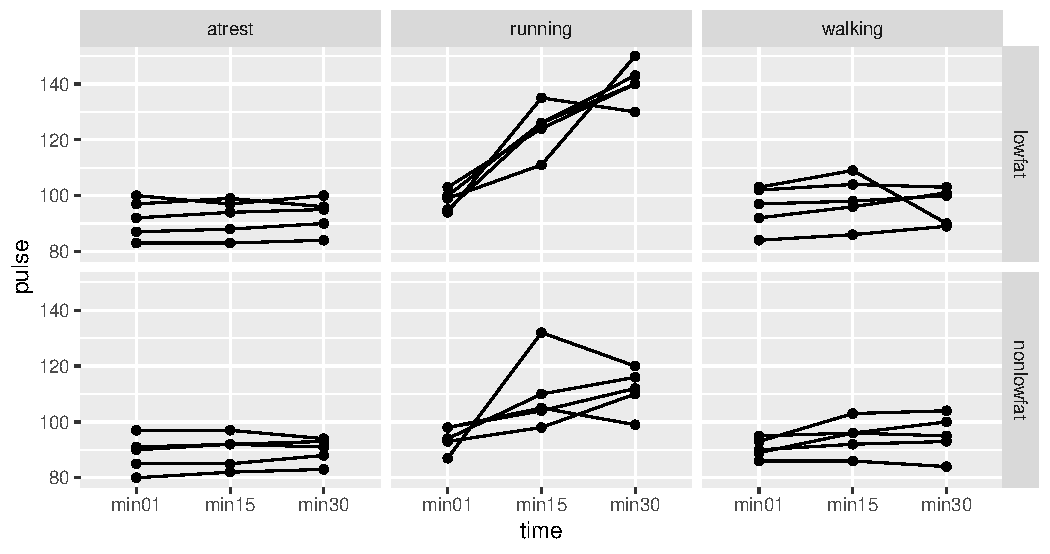
\includegraphics{figure/unnamed-chunk-262-1.pdf}
\caption{plot of chunk unnamed-chunk-262}
\end{figure}

\end{frame}

\begin{frame}[fragile]{Comments on graphs}
\protect\hypertarget{comments-on-graphs}{}

\begin{itemize}
\item
  For subjects who were at rest, no change in pulse rate over time, for
  both diet groups.
\item
  For walking subjects, not much change in pulse rates over time. Maybe
  a small increase on average between 1 and 15 minutes.
\item
  For both running groups, an overall increase in pulse rate over time,
  but the increase is stronger for the \texttt{lowfat} group.
\item
  No consistent effect of diet over all exercise groups.
\item
  No consistent effect of exercise type over both diet groups.
\item
  No consistent effect of time over all diet-exercise type combos.
\end{itemize}

\end{frame}

\begin{frame}[fragile]{``Simple effects'' of diet for the subjects who
ran}
\protect\hypertarget{simple-effects-of-diet-for-the-subjects-who-ran}{}

\begin{itemize}
\item
  Looks as if there is only any substantial time effect for the runners.
  For them, does diet have an effect?
\item
  Pull out only the runners from the wide data:
\end{itemize}

\begin{Shaded}
\begin{Highlighting}[]
\NormalTok{exercise.wide }\OperatorTok
\StringTok{  }\KeywordTok{filter}\NormalTok{(exertype }\OperatorTok{==}\StringTok{ "running"}\NormalTok{) ->}\StringTok{ }\NormalTok{runners.wide}
\end{Highlighting}
\end{Shaded}

\begin{itemize}
\tightlist
\item
  Create response variable and do MANOVA. Some of this looks like
  before, but I have different data now:
\end{itemize}

\footnotesize

\begin{Shaded}
\begin{Highlighting}[]
\NormalTok{response <-}\StringTok{ }\KeywordTok{with}\NormalTok{(runners.wide, }\KeywordTok{cbind}\NormalTok{(min01, min15, min30))}
\NormalTok{runners}\FloatTok{.1}\NormalTok{ <-}\StringTok{ }\KeywordTok{lm}\NormalTok{(response }\OperatorTok{~}\StringTok{ }\NormalTok{diet, }\DataTypeTok{data =}\NormalTok{ runners.wide)}
\NormalTok{times <-}\StringTok{ }\KeywordTok{colnames}\NormalTok{(response)}
\NormalTok{times.df <-}\StringTok{ }\KeywordTok{data.frame}\NormalTok{(times)}
\NormalTok{runners}\FloatTok{.2}\NormalTok{ <-}\StringTok{ }\KeywordTok{Manova}\NormalTok{(runners}\FloatTok{.1}\NormalTok{,}
  \DataTypeTok{idata =}\NormalTok{ times.df,}
  \DataTypeTok{idesign =} \OperatorTok{~}\NormalTok{times}
\NormalTok{)}
\end{Highlighting}
\end{Shaded}

\normalsize

\end{frame}

\begin{frame}[fragile]{Results}
\protect\hypertarget{results-2}{}

\scriptsize

\begin{Shaded}
\begin{Highlighting}[]
\NormalTok{runners}\FloatTok{.2}
\end{Highlighting}
\end{Shaded}

\begin{verbatim}
## 
## Type II Repeated Measures MANOVA Tests: Pillai test statistic
##             Df test stat approx F num Df den Df    Pr(>F)    
## (Intercept)  1   0.99912   9045.3      1      8 1.668e-13 ***
## diet         1   0.84986     45.3      1      8 0.0001482 ***
## times        1   0.92493     43.1      2      7 0.0001159 ***
## diet:times   1   0.68950      7.8      2      7 0.0166807 *  
## ---
## Signif. codes:  0 '***' 0.001 '**' 0.01 '*' 0.05 '.' 0.1 ' ' 1
\end{verbatim}

\normalsize

text under

\begin{itemize}
\item
  The \texttt{diet} by \texttt{time} interaction is still significant
  (at \(\alpha=0.05\)): the effect of time on pulse rates is different
  for the two diets.
\item
  At \(\alpha=0.01\), the interaction is not significant, and then we
  have only two (very) significant main effects of \texttt{diet} and
  \texttt{time}.
\end{itemize}

\end{frame}

\begin{frame}[fragile]{How is the effect of diet different over time?}
\protect\hypertarget{how-is-the-effect-of-diet-different-over-time}{}

\begin{itemize}
\tightlist
\item
  Table of means. Only I need long data for this, so make it (in a
  pipeline):
\end{itemize}

\begin{Shaded}
\begin{Highlighting}[]
\NormalTok{runners.wide }\OperatorTok
\StringTok{  }\KeywordTok{gather}\NormalTok{(time, pulse, min01}\OperatorTok{:}\NormalTok{min30) }\OperatorTok
\StringTok{  }\KeywordTok{group_by}\NormalTok{(time, diet) }\OperatorTok
\StringTok{  }\KeywordTok{summarize}\NormalTok{(}
    \DataTypeTok{mean =} \KeywordTok{mean}\NormalTok{(pulse),}
    \DataTypeTok{sd =} \KeywordTok{sd}\NormalTok{(pulse)}
\NormalTok{  ) ->}\StringTok{ }\NormalTok{summ}
\end{Highlighting}
\end{Shaded}

\begin{verbatim}
## [conflicted] `summarize` found in 2 packages.
## Either pick the one you want with `::` 
## * plyr::summarize
## * dplyr::summarize
## Or declare a preference with `conflict_prefer()`
## * conflict_prefer("summarize", "plyr")
## * conflict_prefer("summarize", "dplyr")
\end{verbatim}

\begin{itemize}
\tightlist
\item
  Result of \texttt{summarize} is data frame, so can save it (and do
  more with it if needed).
\end{itemize}

\end{frame}

\begin{frame}[fragile]{Understanding diet-time interaction}
\protect\hypertarget{understanding-diet-time-interaction}{}

\begin{itemize}
\tightlist
\item
  The summary:
\end{itemize}

\footnotesize

\begin{Shaded}
\begin{Highlighting}[]
\NormalTok{summ}
\end{Highlighting}
\end{Shaded}

\begin{verbatim}
## Error in eval(expr, envir, enclos): object 'summ' not found
\end{verbatim}

\normalsize

\begin{itemize}
\item
  Pulse rates at any given time higher for \texttt{lowfat} (diet
  effect),
\item
  Pulse rates increase over time of exercise (time effect),
\item
  but the \emph{amount by which pulse rate higher} for a diet depends on
  time: \texttt{diet} by \texttt{time} interaction.
\end{itemize}

\end{frame}

\begin{frame}[fragile]{Interaction plot}
\protect\hypertarget{interaction-plot-4}{}

\begin{itemize}
\tightlist
\item
  We went to trouble of finding means by group, so making interaction
  plot is now mainly easy:
\end{itemize}

\begin{Shaded}
\begin{Highlighting}[]
\KeywordTok{ggplot}\NormalTok{(summ, }\KeywordTok{aes}\NormalTok{(}\DataTypeTok{x =}\NormalTok{ time, }\DataTypeTok{y =}\NormalTok{ mean, }\DataTypeTok{colour =}\NormalTok{ diet,}
                 \DataTypeTok{group =}\NormalTok{ diet)) }\OperatorTok{+}\StringTok{ }\KeywordTok{geom_point}\NormalTok{() }\OperatorTok{+}\StringTok{ }\KeywordTok{geom_line}\NormalTok{()}
\end{Highlighting}
\end{Shaded}

\begin{verbatim}
## Error in ggplot(summ, aes(x = time, y = mean, colour = diet, group = diet)): object 'summ' not found
\end{verbatim}

\end{frame}

\begin{frame}{Comment on interaction plot}
\protect\hypertarget{comment-on-interaction-plot}{}

\begin{itemize}
\tightlist
\item
  The lines are not parallel, so there is interaction between diet and
  time for the runners.
\item
  The effect of time on pulse rate is different for the two diets, even
  though all the subjects here were running.
\end{itemize}

\end{frame}

\hypertarget{discriminant-analysis}{%
\section{Discriminant analysis}\label{discriminant-analysis}}

\begin{frame}{Discriminant analysis}
\protect\hypertarget{discriminant-analysis-1}{}

\begin{itemize}
\item
  ANOVA and MANOVA: predict a (counted/measured) response from group
  membership.
\item
  Discriminant analysis: predict group membership based on
  counted/measured variables.
\item
  Covers same ground as logistic regression (and its variations), but
  emphasis on classifying observed data into correct groups.
\item
  Does so by searching for linear combination of original variables that
  best separates data into groups (canonical variables).
\item
  Assumption here that groups are known (for data we have). If trying to
  ``best separate'' data into unknown groups, see \emph{cluster
  analysis} xxx.
\item
  Examples: revisit seed yield and weight data, peanut data,
  professions/activities data; remote-sensing data.
\end{itemize}

\end{frame}

\begin{frame}[fragile]{Packages xxx}
\protect\hypertarget{packages-xxx}{}

\begin{Shaded}
\begin{Highlighting}[]
\KeywordTok{library}\NormalTok{(MASS)}
\KeywordTok{library}\NormalTok{(tidyverse)}
\KeywordTok{library}\NormalTok{(ggrepel)}
\KeywordTok{library}\NormalTok{(ggbiplot)}
\end{Highlighting}
\end{Shaded}

\texttt{ggrepel} allows labelling points on a plot so they don't
overwrite each other.

\end{frame}

\begin{frame}[fragile]{About \texttt{select}}
\protect\hypertarget{about-select}{}

\begin{itemize}
\item
  Both \texttt{dplyr} (in \texttt{tidyverse}) and \texttt{MASS} have a
  function called \texttt{select}, and \emph{they do
  different things}.
\item
  How do you know which \texttt{select} is going to get called?
\item
  With \texttt{library}, the one loaded \emph{last} is visible, and
  others are not.
\item
  Thus we can access the \texttt{select} in \texttt{dplyr} but not the
  one in \texttt{MASS}. If we wanted that one, we'd have to say
  \texttt{MASS::select}.
\item
  I loaded \texttt{MASS} before \texttt{tidyverse}. If I had done it the
  other way around, the \texttt{tidyverse} \texttt{select}, which I want
  to use, would have been the invisible one.
\item
  xxx Alternative: load \texttt{conflicted} package. Any time you load
  two packages containing functions with same name, you get error and
  have to choose between them.
\end{itemize}

\end{frame}

\begin{frame}[fragile]{Example 1: seed yields and weights xxx}
\protect\hypertarget{example-1-seed-yields-and-weights-xxx}{}

\small

\begin{Shaded}
\begin{Highlighting}[]
\NormalTok{my_url <-}\StringTok{ "http://www.utsc.utoronto.ca/~butler/d29/manova1.txt"}
\NormalTok{hilo <-}\StringTok{ }\KeywordTok{read_delim}\NormalTok{(my_url, }\StringTok{" "}\NormalTok{)}
\NormalTok{g <-}\StringTok{ }\KeywordTok{ggplot}\NormalTok{(hilo, }\KeywordTok{aes}\NormalTok{(}
  \DataTypeTok{x =}\NormalTok{ yield, }\DataTypeTok{y =}\NormalTok{ weight,}
  \DataTypeTok{colour =}\NormalTok{ fertilizer}
\NormalTok{)) }\OperatorTok{+}\StringTok{ }\KeywordTok{geom_point}\NormalTok{(}\DataTypeTok{size =} \DecValTok{4}\NormalTok{)}
\end{Highlighting}
\end{Shaded}

\normalsize

\begin{minipage}[t]{0.6\linewidth}
xxx
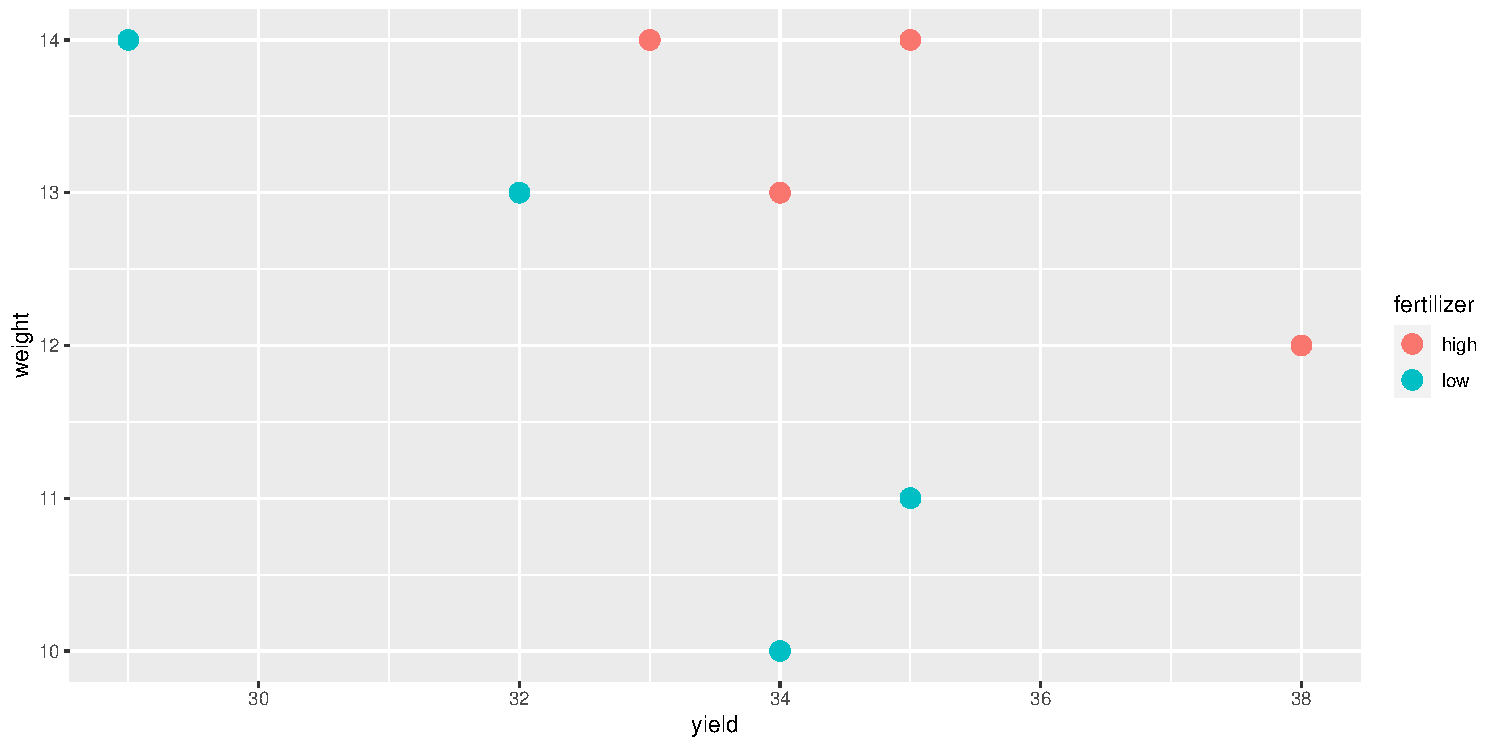
\includegraphics[width=0.6\textwidth]{berzani}
   
\end{minipage}
\begin{minipage}[t]{0.38\linewidth}
\vspace{0.1\textheight}
Recall data from MANOVA: needed a multivariate analysis to find
difference in seed yield and weight based on whether they were high
or low fertilizer.
\end{minipage}

\end{frame}

\begin{frame}[fragile]{Basic discriminant analysis}
\protect\hypertarget{basic-discriminant-analysis}{}

\begin{Shaded}
\begin{Highlighting}[]
\NormalTok{hilo}\FloatTok{.1}\NormalTok{ <-}\StringTok{ }\KeywordTok{lda}\NormalTok{(fertilizer }\OperatorTok{~}\StringTok{ }\NormalTok{yield }\OperatorTok{+}\StringTok{ }\NormalTok{weight, }\DataTypeTok{data =}\NormalTok{ hilo)}
\end{Highlighting}
\end{Shaded}

\begin{itemize}
\item
  Uses \texttt{lda} from package MASS.
\item
  ``Predicting'' group membership from measured variables.
\end{itemize}

\end{frame}

\begin{frame}[fragile]{Output}
\protect\hypertarget{output-3}{}

\small

\begin{Shaded}
\begin{Highlighting}[]
\NormalTok{hilo}\FloatTok{.1}
\end{Highlighting}
\end{Shaded}

\begin{verbatim}
## Call:
## lda(fertilizer ~ yield + weight, data = hilo)
## 
## Prior probabilities of groups:
## high  low 
##  0.5  0.5 
## 
## Group means:
##      yield weight
## high  35.0  13.25
## low   32.5  12.00
## 
## Coefficients of linear discriminants:
##               LD1
## yield  -0.7666761
## weight -1.2513563
\end{verbatim}

\normalsize

\end{frame}

\begin{frame}{Things to take from output}
\protect\hypertarget{things-to-take-from-output}{}

\begin{itemize}
\item
  Group means: high-fertilizer plants have (slightly) higher mean yield
  and weight than low-fertilizer plants.
\item
  ``Coefficients of linear discriminants'': \texttt{LD1,
  LD2,}\ldots are scores constructed from observed variables that best
  separate the groups.
\item
  For any plant, get LD1 score by taking \(-0.76\) times yield plus
  \(-1.25\) times weight, add up, standardize.
\item
  the LD1 coefficients are like slopes:

  \begin{itemize}
  \tightlist
  \item
    if yield higher, LD1 score for a plant lower
  \item
    if weight higher, LD1 score for a plant lower
  \end{itemize}
\item
  High-fertilizer plants have higher yield and weight, thus low
  (negative) LD1 score. Low-fertilizer plants have low yield and weight,
  thus high (positive) LD1 score. xxx
\item
  One LD1 score for each observation. Plot with actual groups.
\end{itemize}

\end{frame}

\begin{frame}{How many linear discriminants?}
\protect\hypertarget{how-many-linear-discriminants}{}

\begin{itemize}
\item
  Smaller of these: xxx

  \begin{itemize}
  \item
    Number of variables
  \item
    Number of groups \emph{minus 1}
  \end{itemize}
\item
  Seed yield and weight: 2 variables, 2 groups, \(\min(2,2-1)=1\).
\end{itemize}

\end{frame}

\begin{frame}[fragile]{Getting LD scores xxx}
\protect\hypertarget{getting-ld-scores-xxx}{}

Feed output from LDA into \texttt{predict}:

\begin{Shaded}
\begin{Highlighting}[]
\NormalTok{hilo.pred <-}\StringTok{ }\KeywordTok{predict}\NormalTok{(hilo}\FloatTok{.1}\NormalTok{)}
\end{Highlighting}
\end{Shaded}

Component \(x\) contains LD score(s), here in descending order:

\footnotesize

\begin{Shaded}
\begin{Highlighting}[]
\NormalTok{d <-}\StringTok{ }\KeywordTok{cbind}\NormalTok{(hilo, hilo.pred}\OperatorTok{$}\NormalTok{x) }\OperatorTok\StringTok{ }\KeywordTok{arrange}\NormalTok{(}\KeywordTok{desc}\NormalTok{(LD1))}
\NormalTok{d}
\end{Highlighting}
\end{Shaded}

\begin{verbatim}
##   fertilizer yield weight        LD1
## 1        low    34     10  3.0931414
## 2        low    29     14  1.9210963
## 3        low    35     11  1.0751090
## 4        low    32     13  0.8724245
## 5       high    34     13 -0.6609276
## 6       high    33     14 -1.1456079
## 7       high    38     12 -2.4762756
## 8       high    35     14 -2.6789600
\end{verbatim}

\normalsize

xxx High fertilizer have yield and weight high, negative LD1 scores.

\end{frame}

\begin{frame}[fragile]{Plotting LD1 scores}
\protect\hypertarget{plotting-ld1-scores}{}

With one LD score, plot against (true) groups, eg. boxplot: xxx

\begin{Shaded}
\begin{Highlighting}[]
\KeywordTok{ggplot}\NormalTok{(d, }\KeywordTok{aes}\NormalTok{(}\DataTypeTok{x =}\NormalTok{ fertilizer, }\DataTypeTok{y =}\NormalTok{ LD1)) }\OperatorTok{+}\StringTok{ }\KeywordTok{geom_boxplot}\NormalTok{()}
\end{Highlighting}
\end{Shaded}

\begin{figure}
\centering
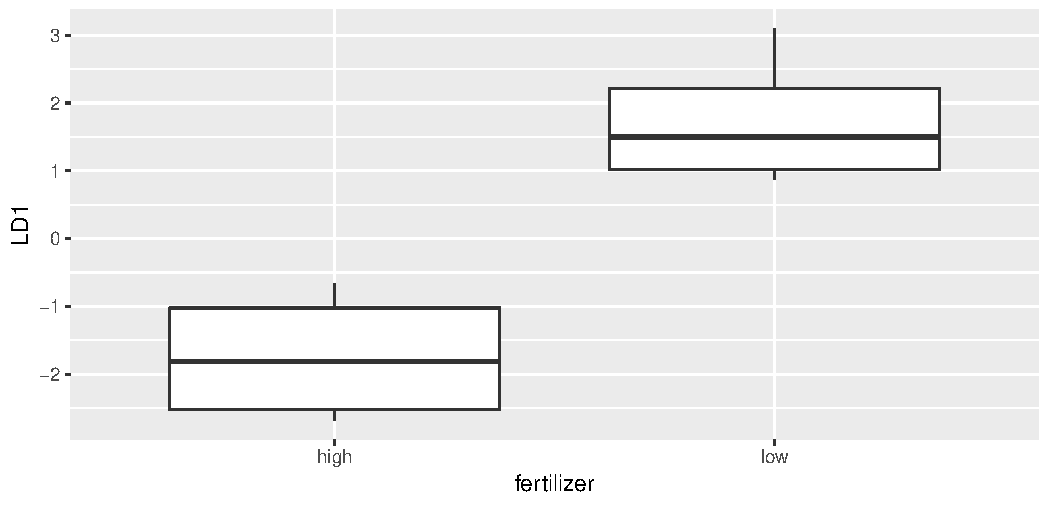
\includegraphics{figure/unnamed-chunk-276-1.pdf}
\caption{plot of chunk unnamed-chunk-276}
\end{figure}

\end{frame}

\begin{frame}[fragile]{Potentially misleading}
\protect\hypertarget{potentially-misleading}{}

\begin{itemize}
\tightlist
\item
  These are like regression slopes: xxx
\end{itemize}

\footnotesize

\begin{Shaded}
\begin{Highlighting}[]
\NormalTok{hilo}\FloatTok{.1}\OperatorTok{$}\NormalTok{scaling}
\end{Highlighting}
\end{Shaded}

\begin{verbatim}
##               LD1
## yield  -0.7666761
## weight -1.2513563
\end{verbatim}

\normalsize

\begin{itemize}
\item
  Reflect change in LD1 score for 1-unit change in variables.
\item
  But one-unit change in variables might not be comparable:
\end{itemize}

\footnotesize

\begin{Shaded}
\begin{Highlighting}[]
\KeywordTok{summary}\NormalTok{(hilo)}
\end{Highlighting}
\end{Shaded}

\begin{verbatim}
##   fertilizer            yield           weight     
##  Length:8           Min.   :29.00   Min.   :10.00  
##  Class :character   1st Qu.:32.75   1st Qu.:11.75  
##  Mode  :character   Median :34.00   Median :13.00  
##                     Mean   :33.75   Mean   :12.62  
##                     3rd Qu.:35.00   3rd Qu.:14.00  
##                     Max.   :38.00   Max.   :14.00
\end{verbatim}

\normalsize

\begin{itemize}
\tightlist
\item
  xxx Here, IQRs \emph{identical}, so 1-unit change in each variable
  means same thing.
\end{itemize}

\end{frame}

\begin{frame}[fragile]{What else is in \texttt{hilo.pred?}}
\protect\hypertarget{what-else-is-in-hilo.pred}{}

\small

\begin{Shaded}
\begin{Highlighting}[]
\KeywordTok{names}\NormalTok{(hilo.pred)}
\end{Highlighting}
\end{Shaded}

\begin{verbatim}
## [1] "class"     "posterior" "x"
\end{verbatim}

\normalsize

\begin{itemize}
\item
  \texttt{class}: predicted fertilizer level (based on values of
  \texttt{yield} and \texttt{weight}).
\item
  \texttt{posterior}: predicted probability of being low or high
  fertilizer given \texttt{yield} and \texttt{weight}.
\end{itemize}

\end{frame}

\begin{frame}[fragile]{Predictions and predicted groups}
\protect\hypertarget{predictions-and-predicted-groups}{}

\ldots based on \texttt{yield} and \texttt{weight}: xxx

\footnotesize

\begin{Shaded}
\begin{Highlighting}[]
\KeywordTok{cbind}\NormalTok{(hilo, }\DataTypeTok{predicted =}\NormalTok{ hilo.pred}\OperatorTok{$}\NormalTok{class)}
\end{Highlighting}
\end{Shaded}

\begin{verbatim}
##   fertilizer yield weight predicted
## 1        low    34     10       low
## 2        low    29     14       low
## 3        low    35     11       low
## 4        low    32     13       low
## 5       high    33     14      high
## 6       high    38     12      high
## 7       high    34     13      high
## 8       high    35     14      high
\end{verbatim}

\begin{Shaded}
\begin{Highlighting}[]
\KeywordTok{table}\NormalTok{(}\DataTypeTok{obs =}\NormalTok{ hilo}\OperatorTok{$}\NormalTok{fertilizer, }\DataTypeTok{pred =}\NormalTok{ hilo.pred}\OperatorTok{$}\NormalTok{class)}
\end{Highlighting}
\end{Shaded}

\begin{verbatim}
##       pred
## obs    high low
##   high    4   0
##   low     0   4
\end{verbatim}

\normalsize

\end{frame}

\begin{frame}{Understanding the predicted groups}
\protect\hypertarget{understanding-the-predicted-groups}{}

\begin{itemize}
\item
  Each predicted fertilizer level is exactly same as observed one
  (perfect prediction).
\item
  Table shows no errors: all values on top-left to bottom-right
  diagonal.
\end{itemize}

\end{frame}

\begin{frame}[fragile]{Posterior probabilities}
\protect\hypertarget{posterior-probabilities}{}

show how clear-cut the classification decisions were:

\small

\begin{Shaded}
\begin{Highlighting}[]
\NormalTok{pp <-}\StringTok{ }\KeywordTok{round}\NormalTok{(hilo.pred}\OperatorTok{$}\NormalTok{posterior, }\DecValTok{4}\NormalTok{)}
\NormalTok{d <-}\StringTok{ }\KeywordTok{cbind}\NormalTok{(hilo, hilo.pred}\OperatorTok{$}\NormalTok{x, pp)}
\NormalTok{d}
\end{Highlighting}
\end{Shaded}

\begin{verbatim}
##   fertilizer yield weight        LD1   high    low
## 1        low    34     10  3.0931414 0.0000 1.0000
## 2        low    29     14  1.9210963 0.0012 0.9988
## 3        low    35     11  1.0751090 0.0232 0.9768
## 4        low    32     13  0.8724245 0.0458 0.9542
## 5       high    33     14 -1.1456079 0.9818 0.0182
## 6       high    38     12 -2.4762756 0.9998 0.0002
## 7       high    34     13 -0.6609276 0.9089 0.0911
## 8       high    35     14 -2.6789600 0.9999 0.0001
\end{verbatim}

\normalsize

Only obs.~7 has any doubt: \texttt{yield} low for a high-fertilizer, but
high \texttt{weight} makes up for it.

\end{frame}

\begin{frame}[fragile]{Example 2: the peanuts xxx}
\protect\hypertarget{example-2-the-peanuts-xxx}{}

\scriptsize

\begin{Shaded}
\begin{Highlighting}[]
\NormalTok{my_url <-}\StringTok{ "http://www.utsc.utoronto.ca/~butler/d29/peanuts.txt"}
\NormalTok{peanuts <-}\StringTok{ }\KeywordTok{read_delim}\NormalTok{(my_url, }\StringTok{" "}\NormalTok{)}
\NormalTok{peanuts}
\end{Highlighting}
\end{Shaded}

\begin{verbatim}
## # A tibble: 12 x 6
##      obs location variety     y   smk     w
##    <dbl>    <dbl>   <dbl> <dbl> <dbl> <dbl>
##  1     1        1       5  195.  153.  51.4
##  2     2        1       5  194.  168.  53.7
##  3     3        2       5  190.  140.  55.5
##  4     4        2       5  180.  121.  44.4
##  5     5        1       6  203   157.  49.8
##  6     6        1       6  196.  166   45.8
##  7     7        2       6  203.  166.  60.4
##  8     8        2       6  198.  162.  54.1
##  9     9        1       8  194.  164.  57.8
## 10    10        1       8  187   165.  58.6
## 11    11        2       8  202.  167.  65  
## 12    12        2       8  200   174.  67.2
\end{verbatim}

\normalsize

\begin{itemize}
\tightlist
\item
  Recall: \texttt{location} and \texttt{variety} both significant in
  MANOVA. Make combo of them (over):
\end{itemize}

\end{frame}

\begin{frame}[fragile]{Location-variety combos xxx}
\protect\hypertarget{location-variety-combos-xxx}{}

\footnotesize

\begin{Shaded}
\begin{Highlighting}[]
\NormalTok{peanuts }\OperatorTok\StringTok{ }\KeywordTok{unite}\NormalTok{(combo, }\KeywordTok{c}\NormalTok{(variety, location)) ->}
\NormalTok{peanuts.combo}
\NormalTok{peanuts.combo}
\end{Highlighting}
\end{Shaded}

\begin{verbatim}
## # A tibble: 12 x 5
##      obs combo     y   smk     w
##    <dbl> <chr> <dbl> <dbl> <dbl>
##  1     1 5_1    195.  153.  51.4
##  2     2 5_1    194.  168.  53.7
##  3     3 5_2    190.  140.  55.5
##  4     4 5_2    180.  121.  44.4
##  5     5 6_1    203   157.  49.8
##  6     6 6_1    196.  166   45.8
##  7     7 6_2    203.  166.  60.4
##  8     8 6_2    198.  162.  54.1
##  9     9 8_1    194.  164.  57.8
## 10    10 8_1    187   165.  58.6
## 11    11 8_2    202.  167.  65  
## 12    12 8_2    200   174.  67.2
\end{verbatim}

\emph{\textbackslash{}1} xxx xxx \normalsize

\end{frame}

\begin{frame}[fragile]{Discriminant analysis}
\protect\hypertarget{discriminant-analysis-2}{}

\small

\begin{Shaded}
\begin{Highlighting}[]
\NormalTok{peanuts}\FloatTok{.1}\NormalTok{ <-}\StringTok{ }\KeywordTok{lda}\NormalTok{(combo }\OperatorTok{~}\StringTok{ }\NormalTok{y }\OperatorTok{+}\StringTok{ }\NormalTok{smk }\OperatorTok{+}\StringTok{ }\NormalTok{w, }\DataTypeTok{data =}\NormalTok{ peanuts.combo)}
\NormalTok{peanuts}\FloatTok{.1}\OperatorTok{$}\NormalTok{scaling}
\end{Highlighting}
\end{Shaded}

\begin{verbatim}
##            LD1         LD2         LD3
## y   -0.4027356 -0.02967881  0.18839237
## smk -0.1727459  0.06794271 -0.09386294
## w    0.5792456  0.16300221  0.07341123
\end{verbatim}

\begin{Shaded}
\begin{Highlighting}[]
\NormalTok{peanuts}\FloatTok{.1}\OperatorTok{$}\NormalTok{svd}
\end{Highlighting}
\end{Shaded}

\begin{verbatim}
## [1] 6.141323 2.428396 1.075589
\end{verbatim}

\normalsize

\begin{itemize}
\tightlist
\item
  Now 3 LDs (3 variables, 6 groups, \(\min(3,6-1)=3\)).
\end{itemize}

\end{frame}

\begin{frame}[fragile]{Comments xxx}
\protect\hypertarget{comments-xxx}{}

\begin{itemize}
\item
  First: relationship of LDs to original variables. Look for coeffs far
  from zero: here,
\item
  high \texttt{LD1} mainly high \texttt{w} or low \texttt{y}.
\item
  high \texttt{LD2} mainly high \texttt{w}.
\item
  \texttt{svd} values show relative importance of LDs: \texttt{LD1} much
  more important than \texttt{LD2}.
\end{itemize}

\end{frame}

\begin{frame}[fragile]{Group means by variable xxx}
\protect\hypertarget{group-means-by-variable-xxx}{}

\begin{Shaded}
\begin{Highlighting}[]
\NormalTok{peanuts}\FloatTok{.1}\OperatorTok{$}\NormalTok{means}
\end{Highlighting}
\end{Shaded}

\begin{verbatim}
##          y    smk     w
## 5_1 194.80 160.40 52.55
## 5_2 185.05 130.30 49.95
## 6_1 199.45 161.40 47.80
## 6_2 200.15 163.95 57.25
## 8_1 190.25 164.80 58.20
## 8_2 200.75 170.30 66.10
\end{verbatim}

\begin{itemize}
\item
  \texttt{5\_2} clearly smallest on \texttt{y}, \texttt{smk}, near
  smallest on \texttt{w}
\item
  \texttt{8\_2} clearly biggest on \texttt{smk}, \texttt{w}, also
  largest on \texttt{y}
\item
  \texttt{8\_1} large on \texttt{w}, small on \texttt{y}.
\end{itemize}

\end{frame}

\begin{frame}[fragile]{The predictions and misclassification}
\protect\hypertarget{the-predictions-and-misclassification}{}

\begin{Shaded}
\begin{Highlighting}[]
\NormalTok{peanuts.pred <-}\StringTok{ }\KeywordTok{predict}\NormalTok{(peanuts}\FloatTok{.1}\NormalTok{)}
\KeywordTok{table}\NormalTok{(}
  \DataTypeTok{obs =}\NormalTok{ peanuts.combo}\OperatorTok{$}\NormalTok{combo,}
  \DataTypeTok{pred =}\NormalTok{ peanuts.pred}\OperatorTok{$}\NormalTok{class}
\NormalTok{)}
\end{Highlighting}
\end{Shaded}

\begin{verbatim}
##      pred
## obs   5_1 5_2 6_1 6_2 8_1 8_2
##   5_1   2   0   0   0   0   0
##   5_2   0   2   0   0   0   0
##   6_1   0   0   2   0   0   0
##   6_2   1   0   0   1   0   0
##   8_1   0   0   0   0   2   0
##   8_2   0   0   0   0   0   2
\end{verbatim}

Actually classified very well. Only one \texttt{6\_2} classified as a
\texttt{5\_1}, rest all correct.

\end{frame}

\begin{frame}[fragile]{Posterior probabilities xxx}
\protect\hypertarget{posterior-probabilities-xxx}{}

\scriptsize

\begin{Shaded}
\begin{Highlighting}[]
\NormalTok{pp <-}\StringTok{ }\KeywordTok{round}\NormalTok{(peanuts.pred}\OperatorTok{$}\NormalTok{posterior, }\DecValTok{2}\NormalTok{)}
\NormalTok{peanuts.combo }\OperatorTok
\StringTok{  }\KeywordTok{select}\NormalTok{(}\OperatorTok{-}\KeywordTok{c}\NormalTok{(y, smk, w)) }\OperatorTok
\StringTok{  }\KeywordTok{cbind}\NormalTok{(., }\DataTypeTok{pred =}\NormalTok{ peanuts.pred}\OperatorTok{$}\NormalTok{class, pp)}
\end{Highlighting}
\end{Shaded}

\begin{verbatim}
##    obs combo pred  5_1 5_2 6_1  6_2  8_1  8_2
## 1    1   5_1  5_1 0.69   0   0 0.31 0.00 0.00
## 2    2   5_1  5_1 0.73   0   0 0.27 0.00 0.00
## 3    3   5_2  5_2 0.00   1   0 0.00 0.00 0.00
## 4    4   5_2  5_2 0.00   1   0 0.00 0.00 0.00
## 5    5   6_1  6_1 0.00   0   1 0.00 0.00 0.00
## 6    6   6_1  6_1 0.00   0   1 0.00 0.00 0.00
## 7    7   6_2  6_2 0.13   0   0 0.87 0.00 0.00
## 8    8   6_2  5_1 0.53   0   0 0.47 0.00 0.00
## 9    9   8_1  8_1 0.02   0   0 0.02 0.75 0.21
## 10  10   8_1  8_1 0.00   0   0 0.00 0.99 0.01
## 11  11   8_2  8_2 0.00   0   0 0.00 0.03 0.97
## 12  12   8_2  8_2 0.00   0   0 0.00 0.06 0.94
\end{verbatim}

\normalsize

\emph{Some} doubt about which combo each plant belongs in, but not too
much. The one misclassified plant was a close call.

\end{frame}

\begin{frame}[fragile]{Discriminant scores, again}
\protect\hypertarget{discriminant-scores-again}{}

\begin{itemize}
\item
  How are discriminant scores related to original variables?
\item
  Construct data frame with original data and discriminant scores side
  by side: xxx
\end{itemize}

\footnotesize

\begin{Shaded}
\begin{Highlighting}[]
\NormalTok{peanuts}\FloatTok{.1}\OperatorTok{$}\NormalTok{scaling}
\end{Highlighting}
\end{Shaded}

\begin{verbatim}
##            LD1         LD2         LD3
## y   -0.4027356 -0.02967881  0.18839237
## smk -0.1727459  0.06794271 -0.09386294
## w    0.5792456  0.16300221  0.07341123
\end{verbatim}

\begin{Shaded}
\begin{Highlighting}[]
\NormalTok{lds <-}\StringTok{ }\KeywordTok{round}\NormalTok{(peanuts.pred}\OperatorTok{$}\NormalTok{x, }\DecValTok{2}\NormalTok{)}
\NormalTok{mm <-}\StringTok{ }\KeywordTok{with}\NormalTok{(peanuts.combo,}
           \KeywordTok{data.frame}\NormalTok{(combo, y, smk, w, lds))}
\end{Highlighting}
\end{Shaded}

\normalsize

\begin{itemize}
\item
  xxx LD1 positive if \texttt{w} large and/or \texttt{y} small.
\item
  LD2 positive if \texttt{w} large.
\end{itemize}

\end{frame}

\begin{frame}[fragile]{Discriminant scores for data}
\protect\hypertarget{discriminant-scores-for-data}{}

\footnotesize

\begin{Shaded}
\begin{Highlighting}[]
\NormalTok{mm}
\end{Highlighting}
\end{Shaded}

\begin{verbatim}
##    combo     y   smk    w   LD1   LD2   LD3
## 1    5_1 195.3 153.1 51.4 -1.42 -1.01  0.26
## 2    5_1 194.3 167.7 53.7 -2.20  0.38 -1.13
## 3    5_2 189.7 139.5 55.5  5.56 -1.10  0.79
## 4    5_2 180.4 121.1 44.4  6.06 -3.89 -0.05
## 5    6_1 203.0 156.8 49.8 -6.08 -1.25  1.25
## 6    6_1 195.9 166.0 45.8 -7.13 -1.07 -1.24
## 7    6_2 202.7 166.1 60.4 -1.43  1.12  1.10
## 8    6_2 197.6 161.8 54.1 -2.28 -0.05  0.08
## 9    8_1 193.5 164.5 57.8  1.05  0.86 -0.67
## 10   8_1 187.0 165.1 58.6  4.02  1.22 -1.90
## 11   8_2 201.5 166.8 65.0  1.60  1.95  1.15
## 12   8_2 200.0 173.8 67.2  2.27  2.83  0.37
\end{verbatim}

\normalsize

\begin{itemize}
\item
  Obs.~5 and 6 have most negative \texttt{LD1}: large \texttt{y}, small
  \texttt{w}.
\item
  Obs.~4 has most negative \texttt{LD2}: small \texttt{w}.
\end{itemize}

\end{frame}

\begin{frame}[fragile]{Predict typical LD1 scores}
\protect\hypertarget{predict-typical-ld1-scores}{}

First and third quartiles for three response variables:

\begin{Shaded}
\begin{Highlighting}[]
\NormalTok{quartiles <-}\StringTok{ }\NormalTok{peanuts }\OperatorTok
\StringTok{  }\KeywordTok{select}\NormalTok{(y}\OperatorTok{:}\NormalTok{w) }\OperatorTok
\StringTok{  }\KeywordTok{map_df}\NormalTok{(quantile, }\KeywordTok{c}\NormalTok{(}\FloatTok{0.25}\NormalTok{, }\FloatTok{0.75}\NormalTok{))}
\NormalTok{quartiles}
\end{Highlighting}
\end{Shaded}

\begin{verbatim}
## # A tibble: 2 x 3
##       y   smk     w
##   <dbl> <dbl> <dbl>
## 1  193.  156.  51  
## 2  200.  166.  59.0
\end{verbatim}

\begin{Shaded}
\begin{Highlighting}[]
\NormalTok{new <-}\StringTok{ }\KeywordTok{with}\NormalTok{(quartiles, }\KeywordTok{crossing}\NormalTok{(y, smk, w))}
\end{Highlighting}
\end{Shaded}

\end{frame}

\begin{frame}[fragile]{The combinations}
\protect\hypertarget{the-combinations}{}

\begin{Shaded}
\begin{Highlighting}[]
\NormalTok{new}
\end{Highlighting}
\end{Shaded}

\begin{verbatim}
## # A tibble: 8 x 3
##       y   smk     w
##   <dbl> <dbl> <dbl>
## 1  193.  156.  51  
## 2  193.  156.  59.0
## 3  193.  166.  51  
## 4  193.  166.  59.0
## 5  200.  156.  51  
## 6  200.  156.  59.0
## 7  200.  166.  51  
## 8  200.  166.  59.0
\end{verbatim}

\begin{Shaded}
\begin{Highlighting}[]
\NormalTok{pp <-}\StringTok{ }\KeywordTok{predict}\NormalTok{(peanuts}\FloatTok{.1}\NormalTok{, new)}
\end{Highlighting}
\end{Shaded}

\end{frame}

\begin{frame}[fragile]{Predicted typical LD1 scores}
\protect\hypertarget{predicted-typical-ld1-scores}{}

\footnotesize

\begin{Shaded}
\begin{Highlighting}[]
\KeywordTok{cbind}\NormalTok{(new, pp}\OperatorTok{$}\NormalTok{x) }\OperatorTok\StringTok{ }\KeywordTok{arrange}\NormalTok{(LD1)}
\end{Highlighting}
\end{Shaded}

\begin{verbatim}
##         y     smk     w        LD1        LD2         LD3
## 1 200.375 166.275 51.00 -5.9688625 -0.3330095 -0.04523828
## 2 200.375 155.875 51.00 -4.1723048 -1.0396138  0.93093630
## 3 192.550 166.275 51.00 -2.8174566 -0.1007728 -1.51940856
## 4 200.375 166.275 59.05 -1.3059358  0.9791583  0.54572212
## 5 192.550 155.875 51.00 -1.0208989 -0.8073770 -0.54323399
## 6 200.375 155.875 59.05  0.4906219  0.2725540  1.52189670
## 7 192.550 166.275 59.05  1.8454701  1.2113950 -0.92844817
## 8 192.550 155.875 59.05  3.6420278  0.5047907  0.04772641
\end{verbatim}

\normalsize

\begin{itemize}
\item
  Very negative LD1 score with large \texttt{y} and small \texttt{w}
\item
  \texttt{smk} doesn't contribute much to LD1
\item
  Very positive LD1 score with small \texttt{y} and large \texttt{w}.
\item
  Same as we saw from Coefficients of Linear Discriminants.
\end{itemize}

\end{frame}

\begin{frame}[fragile]{Plot LD1 vs.~LD2, labelling by combo}
\protect\hypertarget{plot-ld1-vs.ld2-labelling-by-combo}{}

\begin{Shaded}
\begin{Highlighting}[]
\NormalTok{g <-}\StringTok{ }\KeywordTok{ggplot}\NormalTok{(mm, }\KeywordTok{aes}\NormalTok{(}\DataTypeTok{x =}\NormalTok{ LD1, }\DataTypeTok{y =}\NormalTok{ LD2, }\DataTypeTok{colour =}\NormalTok{ combo, }
                    \DataTypeTok{label =}\NormalTok{ combo)) }\OperatorTok{+}\StringTok{ }\KeywordTok{geom_point}\NormalTok{() }\OperatorTok{+}
\StringTok{  }\KeywordTok{geom_text_repel}\NormalTok{() }\OperatorTok{+}\StringTok{ }\KeywordTok{guides}\NormalTok{(}\DataTypeTok{colour =}\NormalTok{ F)}
\NormalTok{g}
\end{Highlighting}
\end{Shaded}

\begin{figure}
\centering
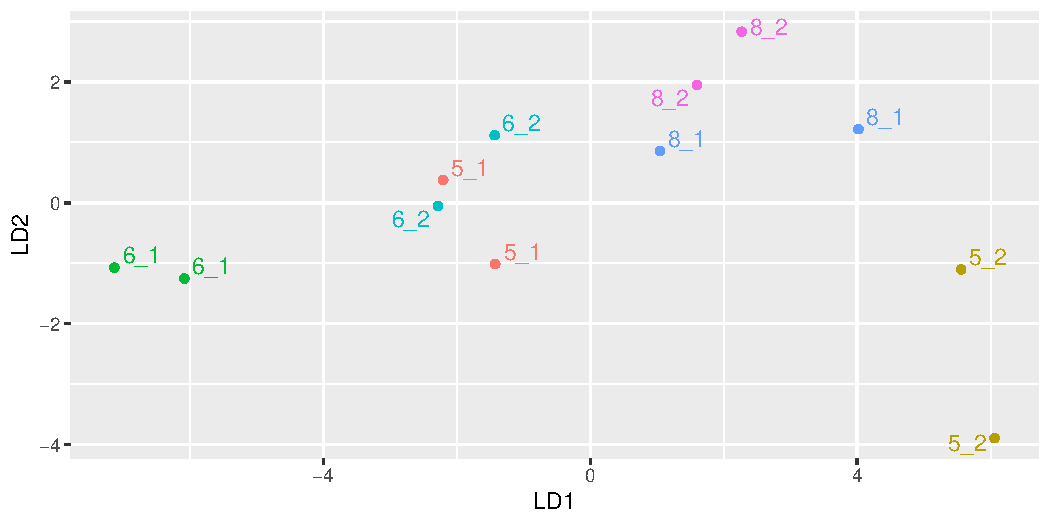
\includegraphics{figure/unnamed-chunk-292-1.pdf}
\caption{plot of chunk unnamed-chunk-292}
\end{figure}

\end{frame}

\begin{frame}[fragile]{``Bi-plot'' from \texttt{ggbiplot} xxx}
\protect\hypertarget{bi-plot-from-ggbiplot-xxx}{}

\begin{Shaded}
\begin{Highlighting}[]
\KeywordTok{ggbiplot}\NormalTok{(peanuts}\FloatTok{.1}\NormalTok{,}
  \DataTypeTok{groups =} \KeywordTok{factor}\NormalTok{(peanuts.combo}\OperatorTok{$}\NormalTok{combo)}
\NormalTok{)}
\end{Highlighting}
\end{Shaded}

\begin{figure}
\centering
\includegraphics{figure/unnamed-chunk-293-1.pdf}
\caption{plot of chunk unnamed-chunk-293}
\end{figure}

\end{frame}

\begin{frame}[fragile]{Installing \texttt{ggbiplot}}
\protect\hypertarget{installing-ggbiplot}{}

\begin{itemize}
\item
  \texttt{ggbiplot} not on CRAN, so usual \texttt{install.packages} will
  not work.
\item
  Install package \texttt{devtools} first (once):
\end{itemize}

\begin{Shaded}
\begin{Highlighting}[]
\KeywordTok{install.packages}\NormalTok{(}\StringTok{"devtools"}\NormalTok{)}
\end{Highlighting}
\end{Shaded}

\begin{itemize}
\tightlist
\item
  Then install \texttt{ggbiplot} (once):
\end{itemize}

\begin{Shaded}
\begin{Highlighting}[]
\KeywordTok{library}\NormalTok{(devtools)}
\KeywordTok{install_github}\NormalTok{(}\StringTok{"vqv/ggbiplot"}\NormalTok{)}
\end{Highlighting}
\end{Shaded}

\end{frame}

\begin{frame}{Cross-validation}
\protect\hypertarget{cross-validation}{}

\begin{itemize}
\item
  So far, have predicted group membership from same data used to form
  the groups --- dishonest!
\item
  Better: \emph{cross-validation}: form groups from all observations
  \emph{except one}, then predict group membership for that left-out
  observation.
\item
  No longer cheating!
\item
  Illustrate with peanuts data again.
\end{itemize}

\end{frame}

\begin{frame}[fragile]{Misclassifications}
\protect\hypertarget{misclassifications}{}

\begin{itemize}
\tightlist
\item
  Fitting and prediction all in one go: xxx text under
\end{itemize}

\small

\begin{Shaded}
\begin{Highlighting}[]
\NormalTok{peanuts.cv <-}\StringTok{ }\KeywordTok{lda}\NormalTok{(combo }\OperatorTok{~}\StringTok{ }\NormalTok{y }\OperatorTok{+}\StringTok{ }\NormalTok{smk }\OperatorTok{+}\StringTok{ }\NormalTok{w,}
  \DataTypeTok{data =}\NormalTok{ peanuts.combo, }\DataTypeTok{CV =}\NormalTok{ T}
\NormalTok{)}
\KeywordTok{table}\NormalTok{(}
  \DataTypeTok{obs =}\NormalTok{ peanuts.combo}\OperatorTok{$}\NormalTok{combo,}
  \DataTypeTok{pred =}\NormalTok{ peanuts.cv}\OperatorTok{$}\NormalTok{class}
\NormalTok{)}
\end{Highlighting}
\end{Shaded}

\begin{verbatim}
##      pred
## obs   5_1 5_2 6_1 6_2 8_1 8_2
##   5_1   0   0   0   2   0   0
##   5_2   0   1   0   0   1   0
##   6_1   0   0   2   0   0   0
##   6_2   1   0   0   1   0   0
##   8_1   0   1   0   0   0   1
##   8_2   0   0   0   0   0   2
\end{verbatim}

\normalsize

\begin{itemize}
\tightlist
\item
  Some more misclassification this time.
\end{itemize}

\end{frame}

\begin{frame}[fragile]{Repeat of LD plot xxx}
\protect\hypertarget{repeat-of-ld-plot-xxx}{}

\begin{Shaded}
\begin{Highlighting}[]
\NormalTok{g}
\end{Highlighting}
\end{Shaded}

\begin{figure}
\centering
\includegraphics{figure/graziani-1.pdf}
\caption{plot of chunk graziani}
\end{figure}

\end{frame}

\begin{frame}[fragile]{Posterior probabilities}
\protect\hypertarget{posterior-probabilities-1}{}

\footnotesize

\begin{Shaded}
\begin{Highlighting}[]
\NormalTok{pp <-}\StringTok{ }\KeywordTok{round}\NormalTok{(peanuts.cv}\OperatorTok{$}\NormalTok{posterior, }\DecValTok{3}\NormalTok{)}
\KeywordTok{data.frame}\NormalTok{(}
  \DataTypeTok{obs =}\NormalTok{ peanuts.combo}\OperatorTok{$}\NormalTok{combo,}
  \DataTypeTok{pred =}\NormalTok{ peanuts.cv}\OperatorTok{$}\NormalTok{class, pp}
\NormalTok{)}
\end{Highlighting}
\end{Shaded}

\begin{verbatim}
##    obs pred  X5_1 X5_2  X6_1  X6_2  X8_1  X8_2
## 1  5_1  6_2 0.162 0.00 0.000 0.838 0.000 0.000
## 2  5_1  6_2 0.200 0.00 0.000 0.799 0.000 0.000
## 3  5_2  8_1 0.000 0.18 0.000 0.000 0.820 0.000
## 4  5_2  5_2 0.000 1.00 0.000 0.000 0.000 0.000
## 5  6_1  6_1 0.194 0.00 0.669 0.137 0.000 0.000
## 6  6_1  6_1 0.000 0.00 1.000 0.000 0.000 0.000
## 7  6_2  6_2 0.325 0.00 0.000 0.667 0.001 0.008
## 8  6_2  5_1 0.821 0.00 0.000 0.179 0.000 0.000
## 9  8_1  8_2 0.000 0.00 0.000 0.000 0.000 1.000
## 10 8_1  5_2 0.000 1.00 0.000 0.000 0.000 0.000
## 11 8_2  8_2 0.001 0.00 0.000 0.004 0.083 0.913
## 12 8_2  8_2 0.000 0.00 0.000 0.000 0.167 0.833
\end{verbatim}

\normalsize

\end{frame}

\begin{frame}[fragile]{Why more misclassification?}
\protect\hypertarget{why-more-misclassification}{}

\begin{itemize}
\item
  When predicting group membership for one observation, only uses the
  \emph{other one} in that group.
\item
  So if two in a pair are far apart, or if two groups overlap, great
  potential for misclassification.
\item
  Groups \texttt{5\_1} and \texttt{6\_2} overlap.
\item
  \texttt{5\_2} closest to \texttt{8\_1}s looks more like an
  \texttt{8\_1} than a \texttt{5\_2} (other one far away).
\item
  \texttt{8\_1}s relatively far apart and close to other things, so one
  appears to be a \texttt{5\_2} and the other an \texttt{8\_2}.
\end{itemize}

\end{frame}

\begin{frame}[fragile]{Example 3: professions and leisure activities}
\protect\hypertarget{example-3-professions-and-leisure-activities}{}

\begin{itemize}
\item
  15 individuals from three different professions (politicians,
  administrators and belly dancers) each participate in four different
  leisure activities: reading, dancing, TV watching and skiing. After
  each activity they rate it on a 0--10 scale.
\item
  Some of the data: xxx
\end{itemize}

\small

\begin{verbatim}
bellydancer 7 10 6 5
bellydancer 8 9 5 7
bellydancer 5 10 5 8
politician 5 5 5 6
politician 4 5 6 5
admin 4 2 2 5
admin 7 1 2 4
admin 6 3 3 3
\end{verbatim}

\normalsize

\begin{itemize}
\item
  How can we best use the scores on the activities to predict a person's
  profession?
\item
  Or, what combination(s) of scores best separate data into profession
  groups?
\end{itemize}

\end{frame}

\begin{frame}[fragile]{Discriminant analysis xxx}
\protect\hypertarget{discriminant-analysis-xxx}{}

\small

\begin{Shaded}
\begin{Highlighting}[]
\NormalTok{my_url <-}\StringTok{ "http://www.utsc.utoronto.ca/~butler/d29/profile.txt"}
\NormalTok{active <-}\StringTok{ }\KeywordTok{read_delim}\NormalTok{(my_url, }\StringTok{" "}\NormalTok{)}
\NormalTok{active}\FloatTok{.1}\NormalTok{ <-}\StringTok{ }\KeywordTok{lda}\NormalTok{(job }\OperatorTok{~}\StringTok{ }\NormalTok{reading }\OperatorTok{+}\StringTok{ }\NormalTok{dance }\OperatorTok{+}\StringTok{ }\NormalTok{tv }\OperatorTok{+}\StringTok{ }\NormalTok{ski, }\DataTypeTok{data =}\NormalTok{ active)}
\NormalTok{active}\FloatTok{.1}\OperatorTok{$}\NormalTok{svd}
\end{Highlighting}
\end{Shaded}

\begin{verbatim}
## [1] 9.856638 3.434555
\end{verbatim}

\begin{Shaded}
\begin{Highlighting}[]
\NormalTok{active}\FloatTok{.1}\OperatorTok{$}\NormalTok{scaling}
\end{Highlighting}
\end{Shaded}

\begin{verbatim}
##                 LD1        LD2
## reading -0.01297465  0.4748081
## dance   -0.95212396  0.4614976
## tv      -0.47417264 -1.2446327
## ski      0.04153684  0.2033122
\end{verbatim}

\normalsize

\begin{itemize}
\item
  Two discriminants, first fair bit more important than second.
\item
  \texttt{LD1} depends (negatively) most on \texttt{dance}, a bit on
  \texttt{tv}. xxx
\item
  \texttt{LD2} depends mostly on \texttt{tv}.
\end{itemize}

\end{frame}

\begin{frame}[fragile]{Misclassification}
\protect\hypertarget{misclassification}{}

\begin{Shaded}
\begin{Highlighting}[]
\NormalTok{active.pred <-}\StringTok{ }\KeywordTok{predict}\NormalTok{(active}\FloatTok{.1}\NormalTok{)}
\KeywordTok{table}\NormalTok{(}\DataTypeTok{obs =}\NormalTok{ active}\OperatorTok{$}\NormalTok{job, }\DataTypeTok{pred =}\NormalTok{ active.pred}\OperatorTok{$}\NormalTok{class)}
\end{Highlighting}
\end{Shaded}

\begin{verbatim}
##              pred
## obs           admin bellydancer politician
##   admin           5           0          0
##   bellydancer     0           5          0
##   politician      0           0          5
\end{verbatim}

Everyone correctly classified.

\end{frame}

\begin{frame}[fragile]{Plotting LDs xxx}
\protect\hypertarget{plotting-lds-xxx}{}

\small

\begin{Shaded}
\begin{Highlighting}[]
\NormalTok{mm <-}\StringTok{ }\KeywordTok{data.frame}\NormalTok{(}\DataTypeTok{job =}\NormalTok{ active}\OperatorTok{$}\NormalTok{job, active.pred}\OperatorTok{$}\NormalTok{x, }\DataTypeTok{person =} \DecValTok{1}\OperatorTok{:}\DecValTok{15}\NormalTok{)}
\NormalTok{g <-}\StringTok{ }\KeywordTok{ggplot}\NormalTok{(mm, }\KeywordTok{aes}\NormalTok{(}\DataTypeTok{x =}\NormalTok{ LD1, }\DataTypeTok{y =}\NormalTok{ LD2, }\DataTypeTok{colour =}\NormalTok{ job, }
                    \DataTypeTok{label =}\NormalTok{ job)) }\OperatorTok{+}\StringTok{ }
\StringTok{  }\KeywordTok{geom_point}\NormalTok{() }\OperatorTok{+}\StringTok{ }\KeywordTok{geom_text_repel}\NormalTok{() }\OperatorTok{+}\StringTok{ }\KeywordTok{guides}\NormalTok{(}\DataTypeTok{colour =}\NormalTok{ F)}
\NormalTok{g}
\end{Highlighting}
\end{Shaded}

\includegraphics{figure/unnamed-chunk-300-1.pdf} \normalsize

\end{frame}

\begin{frame}[fragile]{Biplot xxx}
\protect\hypertarget{biplot-xxx}{}

\begin{Shaded}
\begin{Highlighting}[]
\KeywordTok{ggbiplot}\NormalTok{(active}\FloatTok{.1}\NormalTok{, }\DataTypeTok{groups =}\NormalTok{ active}\OperatorTok{$}\NormalTok{job)}
\end{Highlighting}
\end{Shaded}

\begin{figure}
\centering
\includegraphics{figure/unnamed-chunk-301-1.pdf}
\caption{plot of chunk unnamed-chunk-301}
\end{figure}

\end{frame}

\begin{frame}[fragile]{Comments on plot}
\protect\hypertarget{comments-on-plot}{}

\begin{itemize}
\item
  Groups well separated: bellydancers top left, administrators top
  right, politicians lower middle.
\item
  Bellydancers most negative on \texttt{LD1}: like dancing most.
\item
  Administrators most positive on \texttt{LD1}: like dancing least.
\item
  Politicians most negative on \texttt{LD2}: like TV-watching most.
\end{itemize}

\end{frame}

\begin{frame}[fragile]{Plotting individual \texttt{persons} xxx}
\protect\hypertarget{plotting-individual-persons-xxx}{}

Make \texttt{label} be identifier of person. Now need legend:

\begin{Shaded}
\begin{Highlighting}[]
\KeywordTok{ggplot}\NormalTok{(mm, }\KeywordTok{aes}\NormalTok{(}\DataTypeTok{x =}\NormalTok{ LD1, }\DataTypeTok{y =}\NormalTok{ LD2,  }\DataTypeTok{colour =}\NormalTok{ job, }
               \DataTypeTok{label =}\NormalTok{ person)) }\OperatorTok{+}\StringTok{ }
\StringTok{  }\KeywordTok{geom_point}\NormalTok{() }\OperatorTok{+}\StringTok{ }\KeywordTok{geom_text_repel}\NormalTok{()}
\end{Highlighting}
\end{Shaded}

\begin{figure}
\centering
\includegraphics{figure/unnamed-chunk-302-1.pdf}
\caption{plot of chunk unnamed-chunk-302}
\end{figure}

\end{frame}

\begin{frame}[fragile]{Posterior probabilities}
\protect\hypertarget{posterior-probabilities-2}{}

\scriptsize

\begin{Shaded}
\begin{Highlighting}[]
\NormalTok{pp <-}\StringTok{ }\KeywordTok{round}\NormalTok{(active.pred}\OperatorTok{$}\NormalTok{posterior, }\DecValTok{3}\NormalTok{)}
\KeywordTok{data.frame}\NormalTok{(}\DataTypeTok{obs =}\NormalTok{ active}\OperatorTok{$}\NormalTok{job, }\DataTypeTok{pred =}\NormalTok{ active.pred}\OperatorTok{$}\NormalTok{class, pp)}
\end{Highlighting}
\end{Shaded}

\begin{verbatim}
##            obs        pred admin bellydancer politician
## 1  bellydancer bellydancer 0.000       1.000      0.000
## 2  bellydancer bellydancer 0.000       1.000      0.000
## 3  bellydancer bellydancer 0.000       1.000      0.000
## 4  bellydancer bellydancer 0.000       1.000      0.000
## 5  bellydancer bellydancer 0.000       0.997      0.003
## 6   politician  politician 0.003       0.000      0.997
## 7   politician  politician 0.000       0.000      1.000
## 8   politician  politician 0.000       0.000      1.000
## 9   politician  politician 0.000       0.002      0.998
## 10  politician  politician 0.000       0.000      1.000
## 11       admin       admin 1.000       0.000      0.000
## 12       admin       admin 1.000       0.000      0.000
## 13       admin       admin 1.000       0.000      0.000
## 14       admin       admin 1.000       0.000      0.000
## 15       admin       admin 0.982       0.000      0.018
\end{verbatim}

\normalsize

Not much doubt.

\end{frame}

\begin{frame}[fragile]{Cross-validating the jobs-activities data}
\protect\hypertarget{cross-validating-the-jobs-activities-data}{}

Recall: no need for \texttt{predict}. Just pull out \texttt{class} and
make a table:

\begin{Shaded}
\begin{Highlighting}[]
\NormalTok{active.cv <-}\StringTok{ }\KeywordTok{lda}\NormalTok{(job }\OperatorTok{~}\StringTok{ }\NormalTok{reading }\OperatorTok{+}\StringTok{ }\NormalTok{dance }\OperatorTok{+}\StringTok{ }\NormalTok{tv }\OperatorTok{+}\StringTok{ }\NormalTok{ski,}
  \DataTypeTok{data =}\NormalTok{ active, }\DataTypeTok{CV =}\NormalTok{ T}
\NormalTok{)}
\KeywordTok{table}\NormalTok{(}\DataTypeTok{obs =}\NormalTok{ active}\OperatorTok{$}\NormalTok{job, }\DataTypeTok{pred =}\NormalTok{ active.cv}\OperatorTok{$}\NormalTok{class)}
\end{Highlighting}
\end{Shaded}

\begin{verbatim}
##              pred
## obs           admin bellydancer politician
##   admin           5           0          0
##   bellydancer     0           4          1
##   politician      0           0          5
\end{verbatim}

This time one of the bellydancers was classified as a politician.

\end{frame}

\begin{frame}[fragile]{and look at the posterior probabilities}
\protect\hypertarget{and-look-at-the-posterior-probabilities}{}

picking out the ones where things are not certain:

\footnotesize

\begin{Shaded}
\begin{Highlighting}[]
\NormalTok{pp <-}\StringTok{ }\KeywordTok{round}\NormalTok{(active.cv}\OperatorTok{$}\NormalTok{posterior, }\DecValTok{3}\NormalTok{)}
\KeywordTok{data.frame}\NormalTok{(}\DataTypeTok{obs =}\NormalTok{ active}\OperatorTok{$}\NormalTok{job, }\DataTypeTok{pred =}\NormalTok{ active.cv}\OperatorTok{$}\NormalTok{class, pp) }\OperatorTok
\StringTok{  }\KeywordTok{mutate}\NormalTok{(}\DataTypeTok{max =} \KeywordTok{pmax}\NormalTok{(admin, bellydancer, politician)) }\OperatorTok
\StringTok{  }\KeywordTok{filter}\NormalTok{(max }\OperatorTok{<}\StringTok{ }\FloatTok{0.9995}\NormalTok{)}
\end{Highlighting}
\end{Shaded}

\begin{verbatim}
##           obs       pred admin bellydancer politician   max
## 1 bellydancer politician 0.000       0.001      0.999 0.999
## 2  politician politician 0.006       0.000      0.994 0.994
## 3  politician politician 0.001       0.000      0.999 0.999
## 4  politician politician 0.000       0.009      0.991 0.991
## 5       admin      admin 0.819       0.000      0.181 0.819
\end{verbatim}

\normalsize

\begin{itemize}
\item
  Bellydancer was ``definitely'' a politician!
\item
  One of the administrators might have been a politician too.
\end{itemize}

\end{frame}

\begin{frame}{Why did things get misclassified?}
\protect\hypertarget{why-did-things-get-misclassified}{}

\begin{minipage}[t]{0.7\linewidth}

\includegraphics[width=0.7\textwidth]{nesta}

       
\end{minipage}
\begin{minipage}[t]{0.28\linewidth}


* Go back to plot of discriminant scores:

* one bellydancer much closer to the politicians,

* one administrator a bit closer to the politicians.

\end{minipage}

\end{frame}

\begin{frame}[fragile]{Example 4: remote-sensing data xxx from here}
\protect\hypertarget{example-4-remote-sensing-data-xxx-from-here}{}

\begin{itemize}
\item
  View 38 crops from air, measure 4 variables \texttt{x1-x4}.
\item
  Go back and record what each crop was.
\item
  Can we use the 4 variables to distinguish crops?
\end{itemize}

\end{frame}

\begin{frame}[fragile]{Reading in}
\protect\hypertarget{reading-in-1}{}

\begin{Shaded}
\begin{Highlighting}[]
\NormalTok{my_url <-}\StringTok{ "http://www.utsc.utoronto.ca/~butler/d29/remote-sensing.txt"}
\NormalTok{crops <-}\StringTok{ }\KeywordTok{read_table}\NormalTok{(my_url)}
\end{Highlighting}
\end{Shaded}

\begin{verbatim}
## Parsed with column specification:
## cols(
##   crop = col_character(),
##   x1 = col_double(),
##   x2 = col_double(),
##   x3 = col_double(),
##   x4 = col_double(),
##   cr = col_character()
## )
\end{verbatim}

\end{frame}

\begin{frame}[fragile]{Starting off: number of LDs}
\protect\hypertarget{starting-off-number-of-lds}{}

\begin{Shaded}
\begin{Highlighting}[]
\NormalTok{crops.lda <-}\StringTok{ }\KeywordTok{lda}\NormalTok{(crop }\OperatorTok{~}\StringTok{ }\NormalTok{x1 }\OperatorTok{+}\StringTok{ }\NormalTok{x2 }\OperatorTok{+}\StringTok{ }\NormalTok{x3 }\OperatorTok{+}\StringTok{ }\NormalTok{x4, }\DataTypeTok{data =}\NormalTok{ crops)}
\NormalTok{crops.lda}\OperatorTok{$}\NormalTok{svd}
\end{Highlighting}
\end{Shaded}

\begin{verbatim}
## [1] 2.2858251 1.1866352 0.6394041 0.2303634
\end{verbatim}

\begin{itemize}
\item
  4 LDs (four variables, six groups).
\item
  1st one important, maybe 2nd as well.
\end{itemize}

\end{frame}

\begin{frame}[fragile]{Connecting original variables and LDs}
\protect\hypertarget{connecting-original-variables-and-lds}{}

\begin{Shaded}
\begin{Highlighting}[]
\NormalTok{crops.lda}\OperatorTok{$}\NormalTok{means}
\end{Highlighting}
\end{Shaded}

\begin{verbatim}
##                  x1       x2       x3       x4
## Clover     46.36364 32.63636 34.18182 36.63636
## Corn       15.28571 22.71429 27.42857 33.14286
## Cotton     34.50000 32.66667 35.00000 39.16667
## Soybeans   21.00000 27.00000 23.50000 29.66667
## Sugarbeets 31.00000 32.16667 20.00000 40.50000
\end{verbatim}

\begin{Shaded}
\begin{Highlighting}[]
\KeywordTok{round}\NormalTok{(crops.lda}\OperatorTok{$}\NormalTok{scaling, }\DecValTok{3}\NormalTok{)}
\end{Highlighting}
\end{Shaded}

\begin{verbatim}
##       LD1    LD2    LD3    LD4
## x1 -0.061  0.009 -0.030 -0.015
## x2 -0.025  0.043  0.046  0.055
## x3  0.016 -0.079  0.020  0.009
## x4  0.000 -0.014  0.054 -0.026
\end{verbatim}

\begin{itemize}
\tightlist
\item
  Links groups to original variables to LDs.
\end{itemize}

\end{frame}

\begin{frame}[fragile]{\texttt{LD1\ and\ texttt\{LD2}\}}
\protect\hypertarget{ld1-and-textttld2}{}

\begin{Shaded}
\begin{Highlighting}[]
\KeywordTok{round}\NormalTok{(crops.lda}\OperatorTok{$}\NormalTok{scaling, }\DecValTok{3}\NormalTok{)}
\end{Highlighting}
\end{Shaded}

\begin{verbatim}
##       LD1    LD2    LD3    LD4
## x1 -0.061  0.009 -0.030 -0.015
## x2 -0.025  0.043  0.046  0.055
## x3  0.016 -0.079  0.020  0.009
## x4  0.000 -0.014  0.054 -0.026
\end{verbatim}

\$

\begin{itemize}
\item
  \texttt{LD1} mostly \texttt{x1} (minus), so clover low on
  \texttt{LD1}, corn high.
\item
  \texttt{LD2} \texttt{x3} (minus), \texttt{x2} (plus), so sugarbeets
  should be high on \texttt{LD2}.
\end{itemize}

\end{frame}

\begin{frame}[fragile]{Predictions}
\protect\hypertarget{predictions}{}

\begin{itemize}
\tightlist
\item
  Thus:
\end{itemize}

\footnotesize

\begin{Shaded}
\begin{Highlighting}[]
\NormalTok{crops.pred <-}\StringTok{ }\KeywordTok{predict}\NormalTok{(crops.lda)}
\KeywordTok{table}\NormalTok{(}\DataTypeTok{obs =}\NormalTok{ crops}\OperatorTok{$}\NormalTok{crop, }\DataTypeTok{pred =}\NormalTok{ crops.pred}\OperatorTok{$}\NormalTok{class)}
\end{Highlighting}
\end{Shaded}

\begin{verbatim}
##             pred
## obs          Clover Corn Cotton Soybeans Sugarbeets
##   Clover          6    0      3        0          2
##   Corn            0    6      0        1          0
##   Cotton          3    0      1        2          0
##   Soybeans        0    1      1        3          1
##   Sugarbeets      1    1      0        2          2
\end{verbatim}

\normalsize

\begin{itemize}
\item
  Not very good, eg. only 6 of 11 \texttt{Clover} classified correctly.
\item
  Set up for plot:
\end{itemize}

\begin{Shaded}
\begin{Highlighting}[]
\NormalTok{mm <-}\StringTok{ }\KeywordTok{data.frame}\NormalTok{(}\DataTypeTok{crop =}\NormalTok{ crops}\OperatorTok{$}\NormalTok{crop, crops.pred}\OperatorTok{$}\NormalTok{x)}
\end{Highlighting}
\end{Shaded}

\end{frame}

\begin{frame}[fragile]{Plotting the LDs}
\protect\hypertarget{plotting-the-lds}{}

\begin{Shaded}
\begin{Highlighting}[]
\KeywordTok{ggplot}\NormalTok{(mm, }\KeywordTok{aes}\NormalTok{(}\DataTypeTok{x =}\NormalTok{ LD1, }\DataTypeTok{y =}\NormalTok{ LD2, }\DataTypeTok{colour =}\NormalTok{ crop)) }\OperatorTok{+}
\StringTok{  }\KeywordTok{geom_point}\NormalTok{()}
\end{Highlighting}
\end{Shaded}

\begin{figure}
\centering
\includegraphics{figure/piacentini-1.pdf}
\caption{plot of chunk piacentini}
\end{figure}

\end{frame}

\begin{frame}[fragile]{Biplot}
\protect\hypertarget{biplot}{}

\begin{Shaded}
\begin{Highlighting}[]
\KeywordTok{ggbiplot}\NormalTok{(crops.lda, }\DataTypeTok{groups =}\NormalTok{ crops}\OperatorTok{$}\NormalTok{crop)}
\end{Highlighting}
\end{Shaded}

\begin{figure}
\centering
\includegraphics{figure/unnamed-chunk-313-1.pdf}
\caption{plot of chunk unnamed-chunk-313}
\end{figure}

\textbackslash{}begin\{frame\}{[}figure{]}\{Comments\}

\begin{itemize}
\item
  Corn high on LD1 (right).
\item
  Clover all over the place, but mostly low on LD1 (left).
\item
  Sugarbeets tend to be high on LD2.
\item
  Cotton tends to be low on LD2.
\item
  Very mixed up.
\end{itemize}

\end{frame}

\begin{frame}[fragile]{Try removing Clover}
\protect\hypertarget{try-removing-clover}{}

\begin{itemize}
\tightlist
\item
  the \texttt{dplyr} way:
\end{itemize}

\begin{Shaded}
\begin{Highlighting}[]
\NormalTok{crops }\OperatorTok\StringTok{ }\KeywordTok{filter}\NormalTok{(crop }\OperatorTok{!=}\StringTok{ "Clover"}\NormalTok{) ->}\StringTok{ }\NormalTok{crops2}
\NormalTok{crops2.lda <-}\StringTok{ }\KeywordTok{lda}\NormalTok{(crop }\OperatorTok{~}\StringTok{ }\NormalTok{x1 }\OperatorTok{+}\StringTok{ }\NormalTok{x2 }\OperatorTok{+}\StringTok{ }\NormalTok{x3 }\OperatorTok{+}\StringTok{ }\NormalTok{x4, }\DataTypeTok{data =}\NormalTok{ crops2)}
\end{Highlighting}
\end{Shaded}

\begin{itemize}
\item
  LDs for \texttt{crops2} will be different from before.
\item
  Concentrate on plot and posterior probs.
\end{itemize}

\begin{Shaded}
\begin{Highlighting}[]
\NormalTok{crops2.pred <-}\StringTok{ }\KeywordTok{predict}\NormalTok{(crops2.lda)}
\NormalTok{mm <-}\StringTok{ }\KeywordTok{data.frame}\NormalTok{(}\DataTypeTok{crop =}\NormalTok{ crops2}\OperatorTok{$}\NormalTok{crop, crops2.pred}\OperatorTok{$}\NormalTok{x)}
\end{Highlighting}
\end{Shaded}

\end{frame}

\begin{frame}[fragile]{\texttt{lda\ output}}
\protect\hypertarget{lda-output}{}

Different from before:

\footnotesize

\begin{Shaded}
\begin{Highlighting}[]
\NormalTok{crops2.lda}\OperatorTok{$}\NormalTok{means}
\end{Highlighting}
\end{Shaded}

\begin{verbatim}
##                  x1       x2       x3       x4
## Corn       15.28571 22.71429 27.42857 33.14286
## Cotton     34.50000 32.66667 35.00000 39.16667
## Soybeans   21.00000 27.00000 23.50000 29.66667
## Sugarbeets 31.00000 32.16667 20.00000 40.50000
\end{verbatim}

\begin{Shaded}
\begin{Highlighting}[]
\NormalTok{crops2.lda}\OperatorTok{$}\NormalTok{svd}
\end{Highlighting}
\end{Shaded}

\begin{verbatim}
## [1] 3.3639389 1.6054750 0.4180292
\end{verbatim}

\begin{Shaded}
\begin{Highlighting}[]
\NormalTok{crops2.lda}\OperatorTok{$}\NormalTok{scaling}
\end{Highlighting}
\end{Shaded}

\begin{verbatim}
##            LD1          LD2           LD3
## x1  0.14077479  0.007780184 -0.0312610362
## x2  0.03006972  0.007318386  0.0085401510
## x3 -0.06363974 -0.099520895 -0.0005309869
## x4 -0.00677414 -0.035612707  0.0577718649
\end{verbatim}

\normalsize

\end{frame}

\begin{frame}[fragile]{Plot}
\protect\hypertarget{plot}{}

A bit more clustered:

\begin{Shaded}
\begin{Highlighting}[]
\KeywordTok{ggplot}\NormalTok{(mm, }\KeywordTok{aes}\NormalTok{(}\DataTypeTok{x =}\NormalTok{ LD1, }\DataTypeTok{y =}\NormalTok{ LD2, }\DataTypeTok{colour =}\NormalTok{ crop)) }\OperatorTok{+}
\StringTok{  }\KeywordTok{geom_point}\NormalTok{()}
\end{Highlighting}
\end{Shaded}

\begin{figure}
\centering
\includegraphics{figure/nedved-1.pdf}
\caption{plot of chunk nedved}
\end{figure}

\end{frame}

\begin{frame}[fragile]{Biplot}
\protect\hypertarget{biplot-1}{}

\begin{Shaded}
\begin{Highlighting}[]
\KeywordTok{ggbiplot}\NormalTok{(crops2.lda, }\DataTypeTok{groups =}\NormalTok{ crops2}\OperatorTok{$}\NormalTok{crop)}
\end{Highlighting}
\end{Shaded}

\begin{figure}
\centering
\includegraphics{figure/unnamed-chunk-317-1.pdf}
\caption{plot of chunk unnamed-chunk-317}
\end{figure}

\end{frame}

\begin{frame}[fragile]{Quality of classification}
\protect\hypertarget{quality-of-classification}{}

\small

\begin{Shaded}
\begin{Highlighting}[]
\KeywordTok{table}\NormalTok{(}\DataTypeTok{obs =}\NormalTok{ crops2}\OperatorTok{$}\NormalTok{crop, }\DataTypeTok{pred =}\NormalTok{ crops2.pred}\OperatorTok{$}\NormalTok{class)}
\end{Highlighting}
\end{Shaded}

\begin{verbatim}
##             pred
## obs          Corn Cotton Soybeans Sugarbeets
##   Corn          6      0        1          0
##   Cotton        0      4        2          0
##   Soybeans      2      0        3          1
##   Sugarbeets    0      0        3          3
\end{verbatim}

\normalsize

Better.

\end{frame}

\begin{frame}[fragile]{Posterior probs, the wrong ones}
\protect\hypertarget{posterior-probs-the-wrong-ones}{}

\emph{\textbackslash{}1} xxx \{\footnotesize  

\begin{Shaded}
\begin{Highlighting}[]
\NormalTok{post <-}\StringTok{ }\KeywordTok{round}\NormalTok{(crops2.pred}\OperatorTok{$}\NormalTok{posterior, }\DecValTok{3}\NormalTok{)}
\KeywordTok{data.frame}\NormalTok{(}\DataTypeTok{obs =}\NormalTok{ crops2}\OperatorTok{$}\NormalTok{crop, }\DataTypeTok{pred =}\NormalTok{ crops2.pred}\OperatorTok{$}\NormalTok{class, post) }\OperatorTok
\StringTok{  }\KeywordTok{filter}\NormalTok{(obs }\OperatorTok{!=}\StringTok{ }\NormalTok{pred)}
\end{Highlighting}
\end{Shaded}

\begin{verbatim}
##          obs       pred  Corn Cotton Soybeans Sugarbeets
## 1       Corn   Soybeans 0.443  0.034    0.494      0.029
## 2   Soybeans Sugarbeets 0.010  0.107    0.299      0.584
## 3   Soybeans       Corn 0.684  0.009    0.296      0.011
## 4   Soybeans       Corn 0.467  0.199    0.287      0.047
## 5     Cotton   Soybeans 0.056  0.241    0.379      0.324
## 6     Cotton   Soybeans 0.066  0.138    0.489      0.306
## 7 Sugarbeets   Soybeans 0.381  0.146    0.395      0.078
## 8 Sugarbeets   Soybeans 0.106  0.144    0.518      0.232
## 9 Sugarbeets   Soybeans 0.088  0.207    0.489      0.216
\end{verbatim}

\}

\begin{itemize}
\item
  These were the misclassified ones, but the posterior probability of
  being correct was not usually too low.
\item
  The correctly-classified ones are not very clear-cut either.
\end{itemize}

\end{frame}

\begin{frame}[fragile]{MANOVA}
\protect\hypertarget{manova}{}

Began discriminant analysis as a followup to MANOVA. Do our variables
significantly separate the crops (excluding Clover)?

\begin{Shaded}
\begin{Highlighting}[]
\NormalTok{response <-}\StringTok{ }\KeywordTok{with}\NormalTok{(crops2, }\KeywordTok{cbind}\NormalTok{(x1, x2, x3, x4))}
\NormalTok{crops2.manova <-}\StringTok{ }\KeywordTok{manova}\NormalTok{(response }\OperatorTok{~}\StringTok{ }\NormalTok{crop, }\DataTypeTok{data =}\NormalTok{ crops2)}
\KeywordTok{summary}\NormalTok{(crops2.manova)}
\end{Highlighting}
\end{Shaded}

\begin{verbatim}
##           Df Pillai approx F num Df den Df  Pr(>F)  
## crop       3 0.9113   2.1815     12     60 0.02416 *
## Residuals 21                                        
## ---
## Signif. codes:  
## 0 '***' 0.001 '**' 0.01 '*' 0.05 '.' 0.1 ' ' 1
\end{verbatim}

Yes, at least one of the crops differs (in means) from the others. So it
is worth doing this analysis.

We did this the wrong way around, though!

\end{frame}

\begin{frame}[fragile]{The right way around}
\protect\hypertarget{the-right-way-around}{}

\begin{itemize}
\item
  \emph{First}, do a MANOVA to see whether any of the groups differ
  significantly on any of the variables.
\item
  \emph{If the MANOVA is significant}, do a discriminant analysis in the
  hopes of understanding how the groups are different.
\item
  For remote-sensing data (without Clover):
\item
  LD1 a fair bit more important than LD2 (definitely ignore LD3).
\item
  LD1 depends mostly on \texttt{x1}, on which Cotton was high and Corn
  was low.
\item
  Discriminant analysis in MANOVA plays the same kind of role that Tukey
  does in ANOVA.
\end{itemize}

\begin{verbatim}
## Error in FUN(X[[i]], ...): invalid 'name' argument
\end{verbatim}

\end{frame}

\end{document}
